% Paytm Hisaab -- buildathon pitch deck
%
% Compile with XeLaTeX (needed for the rupee sign and the Kannada line):
%
%   cd pitch
%   xelatex hisaab-pitch.tex                          -> hisaab-pitch.pdf  (slides)
%   xelatex -jobname=hisaab-pitch-notes "\def\shownotes{1}% Paytm Hisaab -- buildathon pitch deck
%
% Compile with XeLaTeX (needed for the rupee sign and the Kannada line):
%
%   cd pitch
%   xelatex hisaab-pitch.tex                          -> hisaab-pitch.pdf  (slides)
%   xelatex -jobname=hisaab-pitch-notes "\def\shownotes{1}% Paytm Hisaab -- buildathon pitch deck
%
% Compile with XeLaTeX (needed for the rupee sign and the Kannada line):
%
%   cd pitch
%   xelatex hisaab-pitch.tex                          -> hisaab-pitch.pdf  (slides)
%   xelatex -jobname=hisaab-pitch-notes "\def\shownotes{1}% Paytm Hisaab -- buildathon pitch deck
%
% Compile with XeLaTeX (needed for the rupee sign and the Kannada line):
%
%   cd pitch
%   xelatex hisaab-pitch.tex                          -> hisaab-pitch.pdf  (slides)
%   xelatex -jobname=hisaab-pitch-notes "\def\shownotes{1}\input{hisaab-pitch.tex}"
%                                                     -> speaker notes, one page per slide
%
% Speaker notes live in the \note{} after each frame, so they cannot drift
% out of sync with the slides. Build both with: ./build.sh
%
% Fonts: Segoe UI + Nirmala UI (both ship with Windows). On another OS the
% deck still builds -- it falls back to the default sans and drops the
% Kannada styling.
\documentclass[aspectratio=169,10pt]{beamer}

\usepackage{fontspec}
\usepackage{tikz}
\usepackage{booktabs}
\usepackage{array}
\newcolumntype{L}[1]{>{\raggedright\arraybackslash}p{#1}}
\usepackage{graphicx}
\usetikzlibrary{calc,positioning,arrows.meta}

\graphicspath{{./}{../}}

% ---------- fonts ----------
\IfFontExistsTF{Segoe UI}{\setsansfont{Segoe UI}}{}
\IfFontExistsTF{Nirmala UI}{%
  \newfontfamily\kn[Script=Kannada]{Nirmala UI}}{%
  \newcommand{\kn}{}}
\renewcommand{\familydefault}{\sfdefault}

% ragged, unhyphenated text inside the narrow cards
\hyphenpenalty=10000
\exhyphenpenalty=10000
\emergencystretch=3em
\hbadness=10000

% ---------- palette (taken from the product mock) ----------
\definecolor{navy}{HTML}{002970}
\definecolor{ptmcyan}{HTML}{00BAF2}
\definecolor{ink}{HTML}{0F172A}
\definecolor{muted}{HTML}{64748B}
\definecolor{good}{HTML}{15803D}
\definecolor{bad}{HTML}{DC2626}
\definecolor{amber}{HTML}{B45309}
\definecolor{tint}{HTML}{EAF4FD}
\definecolor{hairline}{HTML}{DBE7F3}

% ---------- theme ----------
\usetheme{default}
\usecolortheme{default}
\setbeamertemplate{navigation symbols}{}
\setbeamersize{text margin left=0.85cm,text margin right=0.85cm}
\setbeamercolor{normal text}{fg=ink,bg=white}
\setbeamercolor{frametitle}{fg=navy}
\setbeamercolor{structure}{fg=navy}
\setbeamerfont{frametitle}{size=\large,series=\bfseries}
\setbeamerfont{framesubtitle}{size=\scriptsize}
\setbeamercolor{framesubtitle}{fg=muted}
\setbeamertemplate{frametitle}{%
  \vspace{0.30cm}%
  \usebeamerfont{frametitle}\usebeamercolor[fg]{frametitle}\insertframetitle%
  \ifx\insertframesubtitle\empty\else{\\[-0.15em]\usebeamerfont{framesubtitle}\usebeamercolor[fg]{framesubtitle}\insertframesubtitle}\fi%
  \\[0.1em]{\color{ptmcyan}\rule{1.2cm}{2pt}}\par\vspace{-0.15em}%
}
\setbeamertemplate{footline}{%
  \hbox{\begin{beamercolorbox}[wd=\paperwidth,ht=1.9ex,dp=1.1ex,leftskip=0.85cm,rightskip=0.85cm]{}%
  {\scriptsize\color{muted}Paytm Hisaab\hfill\insertframenumber}%
  \end{beamercolorbox}}%
}
\setbeamerfont{itemize/enumerate body}{size=\normalsize}

% ---------- helpers ----------
\newcommand{\hi}[1]{{\color{navy}\bfseries #1}}
\newcommand{\red}[1]{{\color{bad}\bfseries #1}}
\newcommand{\grn}[1]{{\color{good}\bfseries #1}}
\newcommand{\sub}[1]{{\color{muted}#1}}
\newcommand{\qm}[1]{``#1''}
\newcommand{\bignum}[2]{{\color{navy}\fontsize{22}{24}\selectfont\bfseries #1}\\[0.1em]{\scriptsize\color{muted}#2}}
% a soft rounded card:  \card{width}{body}
\newcommand{\card}[2]{\begin{tikzpicture}%
  \node[rounded corners=4pt,fill=tint,inner sep=8pt,text width=#1,align=left]{#2};%
  \end{tikzpicture}}
% an outlined card:  \ocard{colour}{width}{body}
\newcommand{\ocard}[3]{\begin{tikzpicture}%
  \node[rounded corners=4pt,fill=white,draw=#1,line width=0.9pt,inner sep=8pt,text width=#2,align=left]{#3};%
  \end{tikzpicture}}

% ---------- presenter build ----------
% Set after every colour and template above, so the composed notes page keeps
% the deck's own colours:
%   xelatex -jobname=hisaab-pitch-notes "\def\shownotes{1}\input{hisaab-pitch.tex}"
\ifdefined\shownotes
  \setbeamertemplate{note page}{%
    \usebeamercolor[fg]{normal text}%
    \vspace{0.2em}%
    {\scriptsize\color{muted}Paytm Hisaab \;$\cdot$\; speaker notes}\hfill
    {\scriptsize\color{muted}slide \insertframenumber\ of 15}\par
    \vspace{0.25em}{\color{ptmcyan}\rule{\textwidth}{1.5pt}}\par
    \vspace{0.55em}\footnotesize\raggedright\insertnote\par}
  \setbeameroption{show only notes}
\fi

\begin{document}

% ============================================================ 1. TITLE
{\setbeamertemplate{footline}{}
\begin{frame}[plain]
\vspace{0.9cm}
\begin{center}
{\fontsize{38}{42}\selectfont\bfseries\color{navy}Paytm\;\color{ink}Hisaab}\\[0.45em]
{\Large\color{muted}Every rupee, on your side.}\\[0.9em]
{\color{ptmcyan}\rule{2.8cm}{2.5pt}}\\[0.9em]
{\large\color{ink}The agent that lets a merchant account for their own money}\\[0.15em]
{\large\color{ink}when someone in authority demands an explanation.}\\[1.3em]
{\small\color{muted}Agent Labs Buildathon \;$\cdot$\; Phinite $\times$ Paytm \;$\cdot$\; Track 2: AI for Small Businesses}
\end{center}
\note{{\color{navy}\bfseries\normalsize 1.~Title}\par\vspace{0.55em}\textbf{0:10 --- open cold.} Do not read the title or the tagline off the slide.
\\[0.4em]
Say: \emph{``I want to tell you about a man in Haveri who opened an envelope.''} Then advance.
\\[0.4em]
Nothing on this slide needs explaining. The tagline lands at the end, not here.}
\end{frame}}

% ============================================================ 2. STORY
\begin{frame}{Haveri, 2025}{A vegetable vendor opens an envelope}
\vspace{0.05cm}
\begin{columns}[T]
\begin{column}{0.52\textwidth}
\vspace{0.15cm}
He sells vegetables. Vegetables are \hi{exempt} from GST.\\[0.6em]
He also took UPI, because Paytm asked him to.\\[0.6em]
Four years of credits into his account, added up and billed as income:
\begin{center}\vspace{0.1em}{\fontsize{30}{32}\selectfont\bfseries\color{bad}₹29 lakh}\end{center}
\end{column}
\begin{column}{0.44\textwidth}
\ocard{hairline}{5.4cm}{\centering
  {\color{muted}\scriptsize Within weeks, on shutters across Karnataka:}\\[0.6em]
  {\fontsize{20}{23}\selectfont\bfseries\color{ink}\qm{No UPI.\\ Cash only.}}\\[0.6em]
  {\color{muted}\scriptsize A statewide boycott, by the merchants who had just adopted it.}}
\end{column}
\end{columns}
\vspace{0.25cm}
\hspace{0.1cm}{\small\sub{Withdrawn for the traders who could \emph{show} what they sold. Most could not. And tax is no longer the only authority asking.}}
\note{{\color{navy}\bfseries\normalsize 2.~Haveri, 2025}\par\vspace{0.55em}\textbf{0:45 --- the hook. Tell it, do not summarise it.}
\\[0.4em]
Four beats, in this order: he sells vegetables; vegetables are exempt from GST;
he took UPI because \emph{we} asked him to; the department added up four years of
credits and sent him a bill for \textbf{₹29 lakh}.
\\[0.4em]
\textbf{Pause on the number.} Then the card: within weeks, shutters across Karnataka
read ``No UPI, cash only.'' Merchants we had just onboarded, boycotting the rail.
\\[0.4em]
Close on the bottom line --- the notices were withdrawn for traders who could
\emph{show} what they sold. Most could not. That verb is the whole product.
\\[0.4em]
\textbf{Then the bridge:} \emph{``and tax is no longer the only authority asking.''}
That sentence is doing the repositioning --- Haveri is not a tax story here, it is
the moment taking digital money became a liability. The sharper version of it is
two slides away.
\\[0.4em]
\textbf{Do not say this is happening right now.} It is 2025. The next slide is
what makes it current, and a judge who knows the episode will respect the distinction.}
\end{frame}

% ============================================================ 3. STILL HAPPENING
\begin{frame}{And this is not a 2025 story}{CAclubindia, last updated 02 September 2026: ten days ago}
\vspace{0.1cm}
\begin{center}

\includegraphics[width=12.4cm]{gst-notices-2026.png}
\end{center}
\vspace{0.35cm}
\card{13.1cm}{\scriptsize\qm{During August 2026, the GST Department issued a significant number of notices covering different financial years and involving a wide range of issues\ldots\ They covered matters such as ITC mismatches, ineligible credit, \hi{differences in turnover}, wrong GST classification or rate, \hi{exemption claims}, Reverse Charge Mechanism\ldots}}
\vspace{0.3cm}

\hspace{0.1cm}{\small Those two categories are the whole content of an evidence pack. And this is the \emph{slower} of the two authorities. The other one freezes the account first.}
\note{{\color{navy}\bfseries\normalsize 3.~And this is not a 2025 story}\par\vspace{0.55em}\textbf{0:25 --- fast. This slide exists to kill one objection.}
\\[0.4em]
Say: \emph{``That was last year. This was published ten days ago.''}
\\[0.4em]
Do not read the quote. Point at the two bolded phrases only ---
\textbf{differences in turnover} and \textbf{exemption claims} --- and say those
two categories are the entire content of what we build.
\\[0.4em]
\textbf{Land on the last line and move.} It is the handoff into the police
slide: this is the slower authority. The other one freezes first and asks
afterwards. Do not linger here --- tax is no longer the headline.}
\end{frame}

% ============================================================ 4. THE TRAP
\begin{frame}{Every rupee a merchant receives is now evidence}{Today it is only ever used against them}
\vspace{0.05cm}
\begin{columns}[T]
\begin{column}{0.47\textwidth}
\ocard{bad}{6.0cm}{{\bfseries\color{bad}The cyber-crime police}\\[0.35em]
\scriptsize Fraud money layers through accounts within minutes. The shop at the end of the chain, the one that sold someone a watermelon, is frozen. It did nothing wrong, is not named in the FIR, and finds out when a payment declines.}
\end{column}
\begin{column}{0.47\textwidth}
\card{6.1cm}{{\bfseries\color{navy}The tax department}\\[0.35em]
\scriptsize Compares UPI collections against filed returns and bills the difference. Registered traders too, with QR, wallet, card and cash deposits all in scope.}
\end{column}
\end{columns}
\vspace{0.4cm}
\begin{center}
{\large Both demand the same artefact: \hi{what was each rupee, actually?}}\\[0.3em]
{\small\color{muted}Paytm already sees more of this than anyone. What is missing is the \emph{merchant's own answer}, captured when it is still knowable.}
\end{center}
\vspace{0.15cm}
{\color{hairline}\hrule height 1pt}
\vspace{0.35em}
\hspace{0.05cm}{\scriptsize\bfseries\color{bad}What it costs Paytm:}~{\scriptsize a frozen merchant stops transacting that morning. A frightened one takes the QR down for good. Dead Soundbox, zero GMV, no lending origination.}
\note{{\color{navy}\bfseries\normalsize 4.~Every rupee is now evidence}\par\vspace{0.55em}\textbf{0:40 --- two authorities, one unanswerable question.}
\\[0.4em]
\textbf{Left card first and give it the time.} Fraud money layers within minutes,
and the shop at the end of the chain, \emph{the one that sold someone a watermelon},
gets frozen. It did nothing wrong, it is not named in the FIR, and it finds out
when a payment declines. Use the watermelon.
\\[0.4em]
Right card briskly: the department reconciles collections against filed returns
and bills the difference. One sentence, then move.
\\[0.4em]
Then the pivot: both demand the same artefact --- what was each rupee, actually.
\\[0.4em]
\textbf{Say the grey line as written.} We do \emph{not} claim Paytm does nothing
with this data --- it tags plenty. The gap is the merchant's own answer, captured
when it is still knowable. Claiming otherwise in this room gets corrected.
\\[0.4em]
\textbf{Slow down for the red line.} This is the business case, not a footnote:
a frozen merchant stops transacting that morning, a frightened one takes the QR
down for good. Dead Soundbox, zero GMV, no lending origination.}
\end{frame}

% ============================================================ 5. THE BAR
\begin{frame}{Gross credits are not turnover}{One shop, one year, ₹60.98 lakh of credits}
\vspace{0.1cm}
\begin{center}
\begin{tikzpicture}[x=1cm,y=1cm]
% --- what the notice counts
\node[anchor=west,font=\scriptsize\bfseries,text=bad] at (-0.05,1.80) {WHAT THE NOTICE COUNTS AS TURNOVER};
\fill[bad!85,rounded corners=2pt] (0,1.06) rectangle (11.4,1.60);
\node[font=\small\bfseries,text=white] at (5.7,1.33) {₹60.98 lakh};

% --- what actually happened   (1 lakh = 0.18696 cm, so the bars are the same length)
\node[anchor=west,font=\scriptsize\bfseries,text=navy] at (-0.05,0.66) {WHAT ACTUALLY HAPPENED};
\fill[good!80,rounded corners=2pt]  (0,-0.08)     rectangle (6.001,0.46);
\fill[good!45]                      (6.001,-0.08) rectangle (8.002,0.46);
\fill[ptmcyan!70]                   (8.002,-0.08) rectangle (9.385,0.46);
\fill[navy!55]                      (9.385,-0.08) rectangle (10.451,0.46);
\fill[amber!70]                     (10.451,-0.08)rectangle (11.255,0.46);
\fill[muted!60,rounded corners=2pt] (11.255,-0.08)rectangle (11.4,0.46);

% brackets
\draw[navy,line width=0.8pt] (0,-0.22) -- (0,-0.36) -- (8.002,-0.36) -- (8.002,-0.22);
\node[anchor=north,font=\scriptsize,text=navy,align=center] at (4.0,-0.38)
  {\bfseries ₹42.9L aggregate turnover\quad{\color{muted}\scriptsize exempt ₹32.1L + taxable ₹10.7L}};
\draw[bad,line width=0.8pt] (8.002,-0.22) -- (8.002,-0.36) -- (11.4,-0.36) -- (11.4,-0.22);
\node[anchor=north,font=\scriptsize,text=bad,align=center] at (9.7,-0.38)
  {\bfseries ₹18.1L that is not turnover at all};

% legend
\node[font=\scriptsize,text=ink] at (5.7,-1.02) {%
\textcolor{good!80}{$\blacksquare$}~Exempt sales \quad
\textcolor{good!45}{$\blacksquare$}~Taxable sales \quad
\textcolor{ptmcyan!70}{$\blacksquare$}~Her own accounts ₹7.4L};
\node[font=\scriptsize,text=ink] at (5.7,-1.40) {%
\textcolor{navy!55}{$\blacksquare$}~Family ₹5.7L \quad
\textcolor{amber!70}{$\blacksquare$}~Loans, chit, gifts ₹4.3L \quad
\textcolor{muted!60}{$\blacksquare$}~Refunds \& duplicates ₹0.7L};
\end{tikzpicture}
\end{center}
\vspace{0.15cm}
\hspace{0.1cm}{\small\sub{Personal money does not belong on a business QR. It arrives anyway, reads as turnover, and hides the one credit the police will ask about.}}
\note{{\color{navy}\bfseries\normalsize 5.~Gross credits are not turnover}\par\vspace{0.55em}\textbf{0:45 --- the hinge of the pitch. Let the picture work.}
\\[0.4em]
Say: \emph{``One shop, one year, ₹60.98 lakh of credits. The red bar is what the
notice counts as turnover --- all of it.''}
\\[0.4em]
Then the bottom bar. \textbf{Stop talking for two seconds} and let them read it.
\\[0.4em]
₹42.9L really is turnover, and we say so. ₹18.1L is not: her savings account, her
husband, a chit payout, a double-tap on the Soundbox.
\\[0.4em]
\textbf{Get in front of the obvious objection.} Personal money is not supposed to
touch a business QR. Say so first, then say it arrives anyway --- that is an
observation about merchants, not a loophole we are selling. The rule does not stop
it; it only means no one is keeping a record of it.
\\[0.4em]
\textbf{And close on the second use.} This volume is also why she cannot find the
one credit the police care about. Same bar, same problem, and the freeze slide
pays it off.
\\[0.4em]
If challenged on the numbers: seeded ground truth from our generator, not an
estimate. Accuracy against it is slide 14.}
\end{frame}

% ============================================================ 6. INSIGHT
\begin{frame}{The insight}{Most teams would build the tax tool \emph{or} the fraud tool. They are the same engine.}
\vspace{0.15cm}
\begin{center}
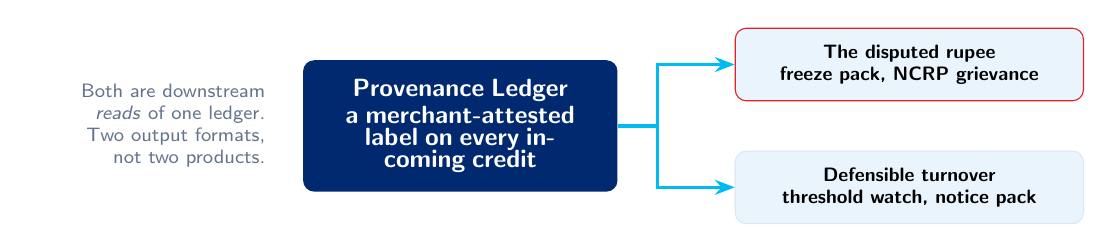
\begin{tikzpicture}[font=\scriptsize]
\node[rounded corners=4pt,fill=navy,text=white,inner sep=7pt,align=center,text width=3.5cm]
  (eng) {\bfseries\small Provenance Ledger\\[0.15em] a merchant-attested label on every incoming credit};
\node[rounded corners=4pt,fill=tint,draw=bad,inner sep=6pt,align=center,text width=4.0cm]
  (tax) at ($(eng.east)+(3.7,0.78)$) {\bfseries The disputed rupee\\ freeze pack, NCRP grievance};
\node[rounded corners=4pt,fill=tint,draw=hairline,inner sep=6pt,align=center,text width=4.0cm]
  (fra) at ($(eng.east)+(3.7,-0.78)$) {\bfseries Defensible turnover\\ threshold watch, notice pack};
\draw[-{Stealth[length=2.5mm]},ptmcyan,line width=1.3pt] (eng.east) -- ++(0.5,0) |- (tax.west);
\draw[-{Stealth[length=2.5mm]},ptmcyan,line width=1.3pt] (eng.east) -- ++(0.5,0) |- (fra.west);
\node[anchor=east,text width=2.9cm,align=right,text=muted] at ($(eng.west)+(-0.35,0)$)
  {Both are downstream \emph{reads} of one ledger. Two output formats, not two products.};
\end{tikzpicture}
\end{center}
\vspace{0.1cm}
\begin{center}
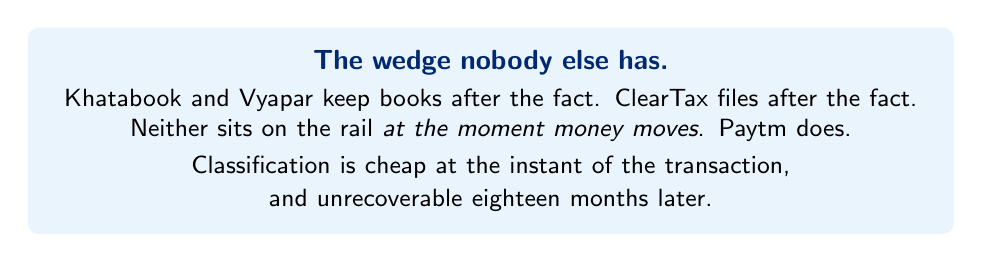
\begin{tikzpicture}\node[rounded corners=4pt,fill=tint,inner sep=8pt,text width=11.2cm,align=center]{
{\bfseries\color{navy}The wedge nobody else has.}\\[0.25em]
\small Khatabook and Vyapar keep books after the fact. ClearTax files after the fact.\\
Neither sits on the rail \emph{at the moment money moves}. Paytm does.\\[0.25em]
\small Classification is cheap at the instant of the transaction,\\ and unrecoverable eighteen months later.
};\end{tikzpicture}
\end{center}
\note{{\color{navy}\bfseries\normalsize 6.~The insight}\par\vspace{0.55em}\textbf{0:40 --- why this is one product, not two.}
\\[0.4em]
Say: \emph{``Most teams would build the fraud tool or the tax tool. They are the
same engine.''} Both are downstream reads of one ledger --- two output formats,
and the freeze pack is the one we lead with.
\\[0.4em]
Then the wedge, and say it slowly because it is the defensible-moat answer:
Khatabook and Vyapar keep books after the fact, ClearTax files after the fact.
Neither sits on the rail at the moment money moves. \textbf{Paytm does.}
\\[0.4em]
Landing line: classification is cheap and accurate at the instant of the
transaction, and unrecoverable eighteen months later when the notice arrives.}
\end{frame}

% ============================================================ 7. THE ENGINE
\begin{frame}{The engine}{Eight tags, one tap}
\vspace{0.15cm}
\begin{columns}[T]
\begin{column}{0.45\textwidth}
{\color{navy}\bfseries\small Every incoming credit gets one tag}\\[0.4em]
{\scriptsize
\begin{tabular}{@{}ll@{}}
\texttt{taxable\_supply}    & ordinary sale \\
\texttt{exempt\_supply}     & vegetables, milk, loose rice \\
\texttt{personal\_transfer} & spouse, parent, sibling \\
\texttt{inter\_account}     & her own money \\
\texttt{refund\_reversal}   & money back from a vendor \\
\texttt{duplicate}          & paid twice, one refunded \\
\texttt{non\_business}      & loan, chit payout, gift \\
{\color{bad}\texttt{unclassified}} & {\color{bad}not enough signal: ask her} \\
\end{tabular}}
\\[0.75em]
{\scriptsize\color{muted}98.6\% are ordinary sales, settled by rules. The agent reasons only about the 1.4\% that need judgement.}
\end{column}
\begin{column}{0.51\textwidth}
\card{6.6cm}{{\bfseries\color{navy}The agent proposes. The merchant attests.}\\[0.4em]
\scriptsize You cannot infer \qm{my husband sent this} from a QR payment. The agent proposes a tag \emph{with its reason}; she confirms with one tap, in Kannada, batched daily.\\[0.45em]
\scriptsize Not a fallback. A ledger she attested \emph{at the time} survives a hearing. An algorithm's guess, made under duress a year later, does not.}
\\[0.55em]
\hspace{0.15cm}\begin{minipage}{6.6cm}
{\bfseries\color{navy}\small Budget: at most 3 questions a day.}\\[0.15em]
{\scriptsize\color{muted}Over a simulated year: \hi{189 questions, median 1.3 a day}. Ask more and the product is dead.}
\end{minipage}
\end{column}
\end{columns}
\note{{\color{navy}\bfseries\normalsize 7.~The engine}\par\vspace{0.55em}\textbf{0:45 --- the mechanism. Do not read the tag list.}
\\[0.4em]
Gesture at the eight tags, say ``eight labels, every incoming credit gets one,''
and move to the right-hand card, which is the real content.
\\[0.4em]
\textbf{The line that matters:} you cannot infer ``my husband sent this'' from a
QR payment. So the agent proposes a tag \emph{with its reason} and she confirms
with one tap. This is not a fallback --- a ledger she attested contemporaneously
survives a hearing; an algorithm's guess produced under duress a year later does not.
\\[0.4em]
Then the budget: at most three questions a day, and we measured 189 across a
year, median 1.3. Ask more than that and the product is dead.
\\[0.4em]
If asked about cost: 98.6\% are ordinary sales settled by rules. The model only
sees the 1.4\% that need judgement.}
\end{frame}

% ============================================================ 8. PRODUCT
\begin{frame}{What the merchant sees}
\vspace{-0.1cm}
\begin{center}
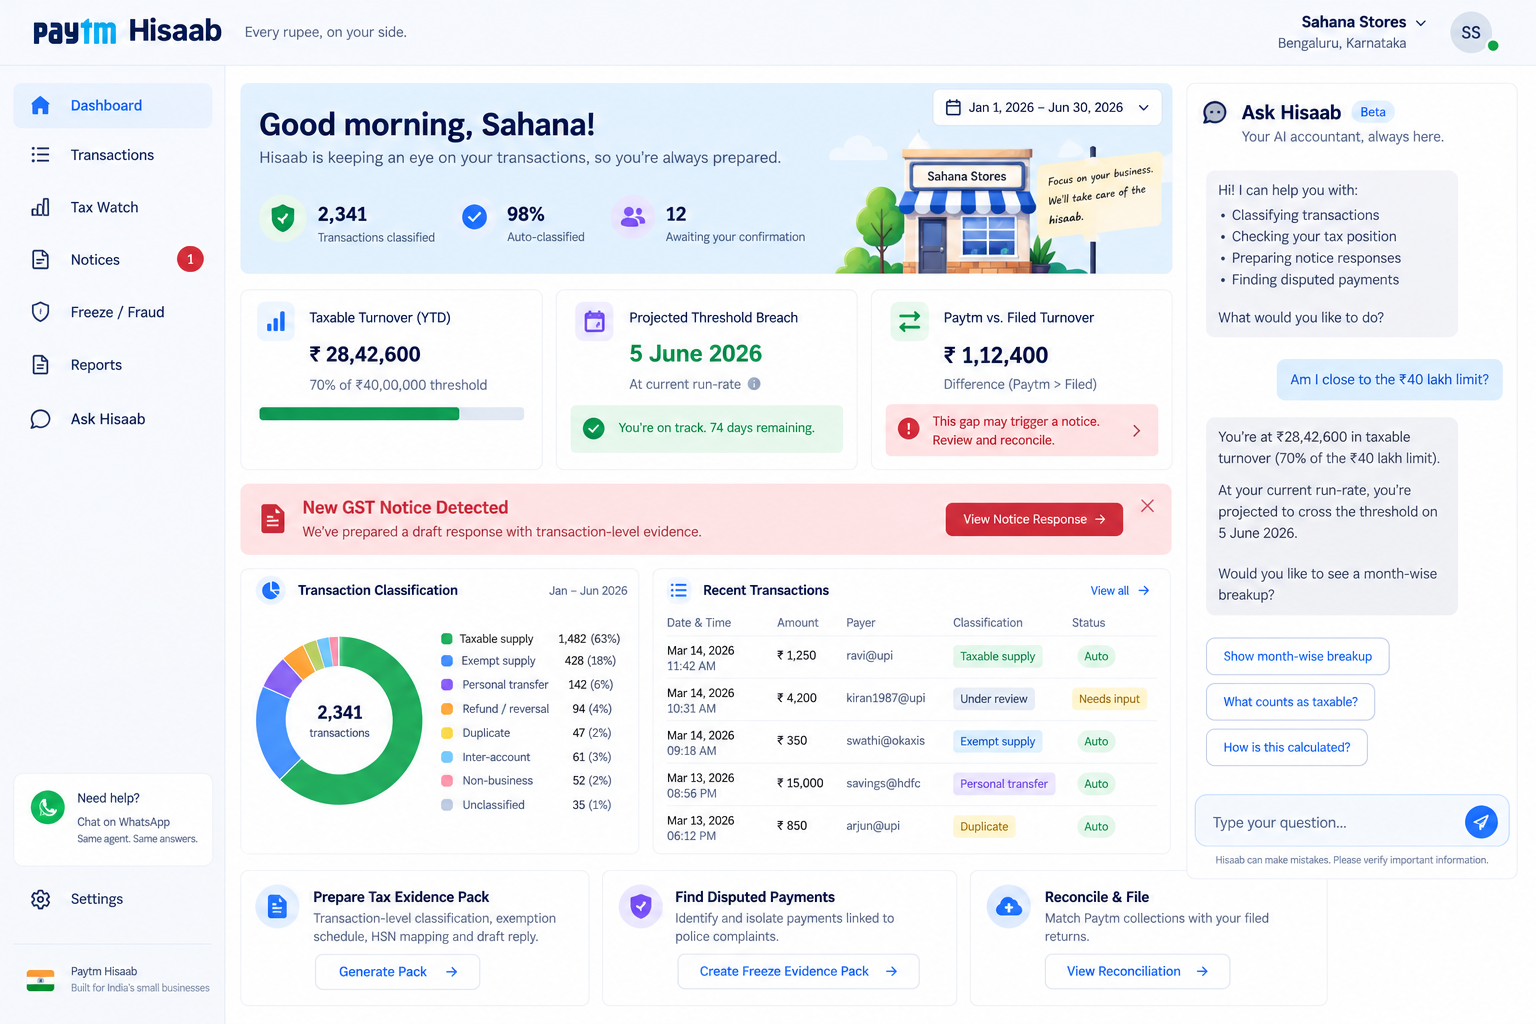
\includegraphics[width=\textwidth,height=0.70\textheight,keepaspectratio]{Paytm-Hisaab_website_look.png}
\end{center}
\vspace{0.1cm}
\hspace{0.05cm}{\scriptsize\color{muted}One surface: what every payment was classified as, how close she is to the threshold, and the packs. The same agent runs on WhatsApp, where she actually is.}
\note{{\color{navy}\bfseries\normalsize 8.~What the merchant sees}\par\vspace{0.55em}\textbf{0:20 --- a glance slide. Do not tour the UI.}
\\[0.4em]
One sentence: everything classified, how close she is to the threshold, and the
packs, on one surface.
\\[0.4em]
Then the WhatsApp point --- the same agent, where she actually is --- and advance.
\\[0.4em]
If someone asks whether this is built: the chat and the tools are live; this
screen is the product surface we are designing toward.}
\end{frame}

% ============================================================ 9. ARCHITECTURE
\begin{frame}{Built on Phinite}{Two agent graphs, four agents, ten deterministic skills}
\vspace{0.15cm}
\begin{columns}[T]
\begin{column}{0.53\textwidth}
{\scriptsize
\begin{tabular}{@{}L{1.75cm}L{4.7cm}@{}}
\multicolumn{2}{@{}l}{\color{navy}\bfseries\small hisaab-watch \;\scriptsize(autonomous: cron + API)}\\
\midrule
Provenance & proposes a tag and a reason for the hard credits \\
Evidence   & assembles packs: freeze evidence, then exemption schedules and HSN \\
\addlinespace[0.6em]
\multicolumn{2}{@{}l}{\color{navy}\bfseries\small hisaab-merchant \;\scriptsize(conversational: chat)}\\
\midrule
Merchant   & the conversation: attestation, alerts, Kannada \\
Escalation & decides when to stop and route to a human CA \\
\bottomrule
\end{tabular}}
\\[0.75em]
{\scriptsize\color{muted}The nightly pass writes its queue to the ledger; the chat reads it when she opens it. Deliberately \emph{not} a graph-to-graph call: a queue that outlives either run is what makes the handoff robust.}
\end{column}
\begin{column}{0.44\textwidth}
\card{5.7cm}{{\bfseries\color{navy}Permissions are the product}\\[0.4em]
\scriptsize Provenance proposes, \red{never commits}.\\[0.25em]
\scriptsize Merchant is the \emph{only} agent that can commit a tag.\\[0.25em]
\scriptsize Evidence is \red{read-only}. It cannot edit a classification to make a pack look better.\\[0.25em]
\scriptsize Escalation can \red{halt} any pack; a human approves.}
\\[0.5em]
\hspace{0.1cm}\begin{minipage}{5.7cm}{\scriptsize\color{muted}Ten tools run live against a hosted service. Every number in a pack traces back, in the trace, to the credit and the attestation behind it.}\end{minipage}
\end{column}
\end{columns}
\note{{\color{navy}\bfseries\normalsize 9.~Built on Phinite}\par\vspace{0.55em}\textbf{0:40 --- for the technical judges.}
\\[0.4em]
Two agent graphs, not four loose agents: \texttt{hisaab-watch} runs autonomously on
cron, \texttt{hisaab-merchant} is the conversation. The nightly pass writes a queue;
the chat reads it when she opens it --- deliberately not a graph-to-graph call,
because a queue that outlives either run is what makes the handoff robust.
\\[0.4em]
\textbf{Spend your time on the right-hand card.} The strongest line in it:
the Evidence agent is read-only --- \emph{the agent that builds the defence cannot
edit the evidence.} And only the Merchant agent can commit an attested tag.
\\[0.4em]
Those are enforced as Phinite tool policies, not conventions, and a denied call
shows up in the trace.}
\end{frame}

% ============================================================ 10. DESIGN DECISIONS
\begin{frame}{Four decisions that make it defensible}
\vspace{0.3cm}
\begin{columns}[T]
\begin{column}{0.48\textwidth}
\card{6.0cm}{{\bfseries\color{navy}1. Arithmetic lives in skills, not the model}\\[0.35em]
\scriptsize Turnover, projections and apportionment are deterministic Python: versioned, testable, traceable. Wrapping arithmetic in an LLM is the standard tell, and the trace would show it.}
\\[0.35em]
\card{6.0cm}{{\bfseries\color{navy}3. Refusing to guess is a feature}\\[0.35em]
\scriptsize An \texttt{unclassified} credit routed to the merchant costs one tap. A confident wrong tag inside an evidence pack is a catastrophe. We report the refusal rate honestly.}
\end{column}
\begin{column}{0.48\textwidth}
\card{6.0cm}{{\bfseries\color{navy}2. Attestation is the promotion boundary}\\[0.35em]
\scriptsize Nothing enters a production pack that the merchant has not confirmed. Sandbox to UAT to prod, with her tap as the gate.}
\\[0.35em]
\card{6.0cm}{{\bfseries\color{navy}4. Ground truth, so accuracy is a number}\\[0.35em]
\scriptsize We simulated a year of a shop's life from a known process, split into what Paytm can see and what really happened. Agents read only the visible half, which is why we quote error bars instead of vibes.}
\end{column}
\end{columns}
\note{{\color{navy}\bfseries\normalsize 10.~Four decisions}\par\vspace{0.55em}\textbf{0:35 --- the slide that separates you from a demo.}
\\[0.4em]
Lead with \#1: all arithmetic is deterministic Python, not model output. Wrapping
arithmetic in an LLM is the standard tell, and the trace would show it.
\\[0.4em]
Then \#3: refusing to guess is a feature. An \texttt{unclassified} credit costs one
tap; a confident wrong tag inside an evidence pack is a catastrophe.
\\[0.4em]
Skim \#2 and \#4 --- one clause each. \#4 is worth a beat if the room is technical:
we generated ground truth, so accuracy is a number instead of a claim.}
\end{frame}

% ============================================================ 11. DEMO / ATTESTATION
\begin{frame}{Demo $\cdot$ Sahana Stores, Jayanagar}{An ordinary Tuesday, before anything goes wrong}
\vspace{0.1cm}
\begin{columns}[T]
\begin{column}{0.48\textwidth}
{\scriptsize\color{muted}Tuesday 10 March. Thirty-nine credits came in over the weekend. The agent asks about \hi{three}.}
\\[0.4em]
\card{5.9cm}{{\kn\scriptsize ಭಾನುವಾರ ರಾತ್ರಿ ₹15,000. ನಿಮ್ಮ ಸ್ವಂತ ಹಣವೇ?}\\[0.25em]
{\color{muted}\scriptsize \qm{₹15,000 at 11:04pm Sunday, from your savings account. Your own money?}}\\[0.35em]
{\scriptsize\color{navy}\fbox{\kn ಹೌದು}\;\fbox{\kn ಇಲ್ಲ}}}
\\[0.4em]
{\scriptsize $\cdot$\; ₹7,500 from her husband, scanned at the shop QR\\[0.25em]
$\cdot$\; ₹4,850 from Raghu Shetty, who has bought twice before. A real sale, and the agent \emph{asks} rather than assumes.}
\\[0.4em]
{\scriptsize\color{muted}The other thirty-six settle silently, and a ₹23 payment nobody can place is left alone.}
\end{column}
\begin{column}{0.48\textwidth}
\ocard{amber}{6.1cm}{{\bfseries\color{amber}And yes, two of those three should not be there}\\[0.35em]
\scriptsize A business QR is not for personal money, and the terms say so. It arrives anyway: family, own top-ups, a chit payout. The rule does not prevent it. It only means \emph{nobody keeps a record of it.}}
\\[0.45em]
{\scriptsize Paytm already reads the signals: channel, linked VPAs, payer history. What no system has is the \hi{merchant's own answer}, given at the time, in her language, and kept.}
\\[0.45em]
{\scriptsize That record is what the next two slides are built from: first for the police, then for the department.}
\end{column}
\end{columns}
\note{{\color{navy}\bfseries\normalsize 11.~Demo --- an ordinary Tuesday (beat 1)}\par\vspace{0.55em}\textbf{0:45 --- or hand over to the live demo here.}
\\[0.4em]
Thirty-nine credits came in over the weekend, the agent asks about \textbf{three}.
Read the Kannada line if you can; otherwise read the gloss under it.
\\[0.4em]
\textbf{Do not hide from the right-hand card --- lead with it.} The mid-review
point was that personal money is not allowed on a business QR. Correct, and we say
so on the slide. The argument is that the rule does not stop it, it only means no
one records it, and an unrecorded credit is what an authority later reads as income.
\\[0.4em]
\textbf{Second half of that card matters just as much.} We are not claiming Paytm
does nothing. It already reads channel, linked VPAs and payer history. What no
system has is her own answer, captured while it is still knowable. That is the
product, and it is a smaller, truer claim than the one we started with.
\\[0.4em]
\textbf{Before going on stage:} confirm the attestation queue is whole ---
\texttt{pending\_total} must be 3. A rehearsal that taps through this beat spends the
queue, and Render needs a clear-cache redeploy to restore it.}
\end{frame}

% ============================================================ 12. DEMO / THE FREEZE
\begin{frame}{Demo $\cdot$ The emergency}{The account is frozen at 09:30 and the supplier payment is due}
\vspace{0.2cm}
\begin{columns}[T]
\begin{column}{0.46\textwidth}
{\scriptsize She sold someone 12kg of onions. That customer was three layers downstream of a fraud victim. She is not named in the FIR, which was filed in another state, and \hi{339 payments} came in that week.}
\\[0.5em]
\card{5.8cm}{{\bfseries\color{navy}The agent isolates it}\\[0.35em]
\scriptsize ₹4,200 on 21 March at 19:47, till POS01. Matched by UTR \emph{and independently} by amount and date.\\[0.3em]
\scriptsize The sale record comes with it: the POS bill, the items, the till and the minute.}
\end{column}
\begin{column}{0.49\textwidth}
\ocard{amber}{6.1cm}{{\bfseries\color{amber}And the decoy it did not choose}\\[0.35em]
\scriptsize A \emph{second} ₹4,200 that same week, from a regular customer. Listed in the pack, and explicitly \emph{not} named as the disputed one. Only the date separates them.}
\\[0.5em]
{\scriptsize Then it drafts the NCRP-CFCFRMS grievance, citing the judgments that only the \emph{disputed amount} should be lien-marked, not the whole account.}
\\[0.5em]
{\scriptsize\color{bad}\bfseries It never asserts that she is innocent.}\\[0.1em]
{\scriptsize\color{muted}Some frozen accounts genuinely are mule accounts. The agent assembles evidence; a human decides. Escalation holds the pack for approval.}
\end{column}
\end{columns}
\note{{\color{navy}\bfseries\normalsize 12.~Demo --- the emergency (beat 4)}\par\vspace{0.55em}\textbf{0:50 --- this is now the lead case. Give it the most time of the three.}
\\[0.4em]
Set the stakes in one sentence: account frozen at half nine, supplier payment due,
339 payments came in that week, and she is not named in the FIR.
\\[0.4em]
\textbf{Why this one leads.} She did nothing wrong and there is no rule she broke.
She sold onions to a customer who turned out to be laundering. Every objection
available against the tax case --- she should not have taken personal money on that
QR, she should have registered --- has no purchase here at all.
\\[0.4em]
The agent isolates ₹4,200 by UTR \emph{and independently} by amount and date, and
brings the POS bill with it --- the items, till POS01, 19:47.
\\[0.4em]
\textbf{The decoy is the point.} A second ₹4,200 that same week from a regular
customer, listed in the pack and explicitly not chosen. Anyone can match an amount;
the pack shows its work.
\\[0.4em]
Finish on the red line: it never asserts she is innocent. Some frozen accounts
genuinely are mule accounts. We assemble evidence; a human decides, and Escalation
holds the pack for approval.}
\end{frame}

% ============================================================ 13. DEMO / TAX
\begin{frame}{Demo $\cdot$ The warning, and the notice}{The same ledger, read for the other authority}
\vspace{0.15cm}
\begin{columns}[T]
\begin{column}{0.38\textwidth}
{\scriptsize\color{muted}Replayed as of 31 January:}
\\[0.35em]
\ocard{good}{4.8cm}{{\bfseries\color{ink}\scriptsize\qm{At your current rate you cross ₹40 lakh around {\color{bad}14 March}. You will need to register.}}\\[0.35em]
{\scriptsize\color{muted}\grn{43 days of warning}, and the date is computed, not typed.}}
\\[0.45em]
{\scriptsize\color{bad}\bfseries This beat is what makes the pitch safe.}\\[0.1em]
{\scriptsize\color{muted}Its first act on the tax side is telling her to register.}
\end{column}
\begin{column}{0.58\textwidth}
{\scriptsize\color{muted}Then the notice arrives, claiming {\color{bad}\bfseries ₹60.98L} of turnover:}
\\[0.3em]
{\scriptsize
\begin{tabular}{@{}lr@{\hskip 1.2em}l@{}}
\multicolumn{2}{@{}l}{\color{navy}\bfseries Aggregate turnover \quad ₹42.2L} & \sub{within \grn{1.6\%} of truth} \\
\midrule
Exempt supplies      & ₹31.3L & \sub{vegetables, loose rice} \\
Taxable supplies     & ₹10.9L & \sub{branded goods, oil, soap} \\
\addlinespace[0.45em]
\multicolumn{2}{@{}l}{\color{navy}\bfseries Not turnover at all \quad ₹18.8L} & \sub{every line traced} \\
\midrule
Her own accounts     & ₹7.4L & \sub{top-ups before supplier runs} \\
Family               & ₹6.1L & \sub{spouse, parent, in-law} \\
Loans, chit, gifts   & ₹4.3L & \sub{chit payout, festival gifts} \\
Refunds, duplicates  & ₹1.0L & \sub{crate returns, double-taps} \\
\bottomrule
\end{tabular}}
\\[0.45em]
{\scriptsize And it says plainly: \hi{the claim is wrong, and you \emph{did} cross ₹40 lakh on 14 March. You must register.}}
\end{column}
\end{columns}
\note{{\color{navy}\bfseries\normalsize 13.~Demo --- the warning and the notice (beats 2 and 3)}\par\vspace{0.55em}\textbf{0:50 --- two tax beats on one slide, deliberately compressed.}
\\[0.4em]
Left: replayed as of 31 January, the agent says she crosses ₹40 lakh around
14 March. \textbf{Say the red line out loud} --- its first act on the tax side is
telling her she owes a registration. That is what stops the room turning hostile.
\\[0.4em]
Right: the notice claims ₹60.98 lakh, and the pack answers it line by line, every
figure traceable to transaction IDs. Then the honest half:
\textbf{the claim is wrong, and she did cross ₹40 lakh, and she must register.}
\\[0.4em]
\textbf{If a judge diffs this against slide 5:} slide 5 shows seeded truth
(₹42.9L), this shows what our system computed (₹42.2L). The 1.6\% between them
\emph{is} the accuracy claim --- say that, do not hedge.
\\[0.4em]
\textbf{If pushed on the personal and own-account lines:} same answer as slide 11.
Those credits should not be on a business QR, they are there anyway, and the
alternative to classifying them is letting them be read as income.}
\end{frame}

% ============================================================ 14. NUMBERS
\begin{frame}{What we can actually prove}{One merchant, one year, 13,267 credits, scored against seeded truth}
\vspace{0.45cm}
\begin{columns}[T]
\begin{column}{0.33\textwidth}
\begin{center}\bignum{1.6\%}{error on aggregate turnover\\ (taxable share within 1\%)}\end{center}
\vspace{0.55cm}
\begin{center}\bignum{43 days}{of warning before the\\ threshold crossing}\end{center}
\end{column}
\begin{column}{0.33\textwidth}
\begin{center}\bignum{1.3 a day}{median questions asked.\\ 189 in a year, never over 3}\end{center}
\vspace{0.55cm}
\begin{center}\bignum{zero}{credits left untagged\\ across the whole year}\end{center}
\end{column}
\begin{column}{0.30\textwidth}
\card{3.8cm}{{\bfseries\color{navy}The honest baseline}\\[0.35em]
\scriptsize A 50-line rules-only classifier gets 99.3\% on sale vs not-a-sale, but catches only \red{77.8\%} of non-sale credits.\\[0.3em]
\scriptsize That residue alone puts two eval merchants on the \emph{wrong side} of ₹40L.\\[0.3em]
\scriptsize Closing it is what the agent plus one tap is for.}
\end{column}
\end{columns}
\vspace{0.45cm}
\hspace{0.1cm}{\scriptsize\color{muted}She corrected the agent 52 times that year. Those corrections are the ledger's strongest evidence, not its failures.}
\note{{\color{navy}\bfseries\normalsize 14.~What we can actually prove}\par\vspace{0.55em}\textbf{0:30 --- do not read all four. Pick two.}
\\[0.4em]
Lead with \textbf{1.6\%} error on turnover and \textbf{1.3 questions a day}. The
other two are there to be read, not narrated.
\\[0.4em]
\textbf{The credibility move is the box on the right} --- volunteer the weakness
before anyone finds it. A rules-only baseline gets 99.3\% on sale vs not-a-sale
but catches only 77.8\% of non-sale credits, and that residue alone puts two eval
merchants on the wrong side of ₹40 lakh. Closing it is what the agent plus one tap is for.
\\[0.4em]
Last line if you have the beat: she corrected the agent 52 times that year, and
those corrections are the ledger's strongest evidence, not its failures.}
\end{frame}

% ============================================================ 15. CLOSE
\begin{frame}{The line we do not cross}{Accuracy, not minimisation}
\vspace{0.3cm}
\begin{columns}[T]
\begin{column}{0.52\textwidth}
{\scriptsize
$\cdot$\; We \hi{never assert innocence} on a freeze. Some accounts really are mule accounts. We assemble evidence; a human decides.\\[0.5em]
$\cdot$\; We \hi{file nothing} with any authority. Artefacts only; the merchant or their CA files.\\[0.5em]
$\cdot$\; We compute what she \hi{genuinely owes} and say so plainly, including \qm{you crossed the threshold, you must register.}\\[0.5em]
$\cdot$\; We \hi{never assert a final liability}. We compute, show the workings, and route to a CA.\\[0.5em]
$\cdot$\; A business QR is \hi{not for personal money}. We do not excuse it. We record it, so it is not read as income.}
\end{column}
\begin{column}{0.44\textwidth}
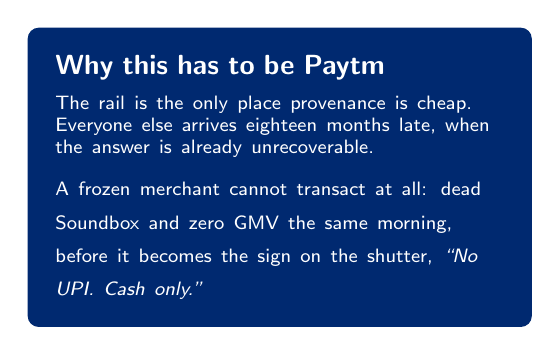
\begin{tikzpicture}\node[rounded corners=4pt,fill=navy,text=white,inner sep=10pt,text width=5.7cm,align=left]{
{\bfseries Why this has to be Paytm}\\[0.45em]
\scriptsize The rail is the only place provenance is cheap. Everyone else arrives eighteen months late, when the answer is already unrecoverable.\\[0.45em]
\scriptsize A frozen merchant cannot transact at all: dead Soundbox and zero GMV the same morning, before it becomes the sign on the shutter, \emph{\qm{No UPI. Cash only.}}
};\end{tikzpicture}
\end{column}
\end{columns}
\vspace{0.4cm}
\begin{center}
{\large\color{navy}\bfseries Paytm Hisaab}\quad{\color{muted}every rupee, on your side.}
\end{center}
\note{{\color{navy}\bfseries\normalsize 15.~The line we do not cross}\par\vspace{0.55em}\textbf{0:30 --- the non-negotiables, fast, then land.}
\\[0.4em]
Run the five bullets at pace. The one to hit is the first: we never assert
innocence on a freeze. The last is the mid-review answer, on the slide on purpose.
\\[0.4em]
Then the navy box: provenance is cheap only on the rail, and a frozen merchant
stops transacting the same morning.
\\[0.4em]
Final line, unhurried: \emph{``Paytm Hisaab. Every rupee, on your side.''} Stop talking.
\\[0.5em]
{\scriptsize
{\color{navy}\bfseries --- Q\&A prep ---}
\\[0.3em]
\textbf{``Merchants may not take personal money on a business QR.''} Correct, and
slide 11 says so before you have to. It arrives anyway, and the alternative to
recording it is letting an authority read it as income. We are not defending the
behaviour --- we are refusing to let it become a liability.
\\[0.3em]
\textbf{``Paytm already tags transactions.''} It does, and we build on that rather
than around it: channel, linked VPAs and payer history feed the rules layer. What
no tag carries is her attestation --- the part an authority accepts, and the only
part she alone can give.
\\[0.3em]
\textbf{``No return mismatch?''} That check needs a \emph{registered} composition
dealer who filed a CMP-08 to disagree with. Ours is unregistered, which is why she
gets a notice at all; the eval split has one with four quarters seeded.
\\[0.3em]
\textbf{``Exempt vs taxable on a QR sale?''} Not per payment. We apportion by value
from that shop's own POS-billed ratio and label it an estimate. Labelling each sale
by its majority side understated taxable turnover threefold.
\\[0.3em]
\textbf{``Four LLM calls in a trenchcoat?''} Everything deterministic is a skill and
four agents is the ceiling. If twenty lines of Python replaces an agent, it should
have been a skill --- the trace shows which is which.
\\[0.3em]
\textbf{``No standing with the police.''} Agreed: Paytm supplies, the merchant
files. By design. Cash sales are real, out of scope, and on the slide.}}
\end{frame}

\end{document}
"
%                                                     -> speaker notes, one page per slide
%
% Speaker notes live in the \note{} after each frame, so they cannot drift
% out of sync with the slides. Build both with: ./build.sh
%
% Fonts: Segoe UI + Nirmala UI (both ship with Windows). On another OS the
% deck still builds -- it falls back to the default sans and drops the
% Kannada styling.
\documentclass[aspectratio=169,10pt]{beamer}

\usepackage{fontspec}
\usepackage{tikz}
\usepackage{booktabs}
\usepackage{array}
\newcolumntype{L}[1]{>{\raggedright\arraybackslash}p{#1}}
\usepackage{graphicx}
\usetikzlibrary{calc,positioning,arrows.meta}

\graphicspath{{./}{../}}

% ---------- fonts ----------
\IfFontExistsTF{Segoe UI}{\setsansfont{Segoe UI}}{}
\IfFontExistsTF{Nirmala UI}{%
  \newfontfamily\kn[Script=Kannada]{Nirmala UI}}{%
  \newcommand{\kn}{}}
\renewcommand{\familydefault}{\sfdefault}

% ragged, unhyphenated text inside the narrow cards
\hyphenpenalty=10000
\exhyphenpenalty=10000
\emergencystretch=3em
\hbadness=10000

% ---------- palette (taken from the product mock) ----------
\definecolor{navy}{HTML}{002970}
\definecolor{ptmcyan}{HTML}{00BAF2}
\definecolor{ink}{HTML}{0F172A}
\definecolor{muted}{HTML}{64748B}
\definecolor{good}{HTML}{15803D}
\definecolor{bad}{HTML}{DC2626}
\definecolor{amber}{HTML}{B45309}
\definecolor{tint}{HTML}{EAF4FD}
\definecolor{hairline}{HTML}{DBE7F3}

% ---------- theme ----------
\usetheme{default}
\usecolortheme{default}
\setbeamertemplate{navigation symbols}{}
\setbeamersize{text margin left=0.85cm,text margin right=0.85cm}
\setbeamercolor{normal text}{fg=ink,bg=white}
\setbeamercolor{frametitle}{fg=navy}
\setbeamercolor{structure}{fg=navy}
\setbeamerfont{frametitle}{size=\large,series=\bfseries}
\setbeamerfont{framesubtitle}{size=\scriptsize}
\setbeamercolor{framesubtitle}{fg=muted}
\setbeamertemplate{frametitle}{%
  \vspace{0.30cm}%
  \usebeamerfont{frametitle}\usebeamercolor[fg]{frametitle}\insertframetitle%
  \ifx\insertframesubtitle\empty\else{\\[-0.15em]\usebeamerfont{framesubtitle}\usebeamercolor[fg]{framesubtitle}\insertframesubtitle}\fi%
  \\[0.1em]{\color{ptmcyan}\rule{1.2cm}{2pt}}\par\vspace{-0.15em}%
}
\setbeamertemplate{footline}{%
  \hbox{\begin{beamercolorbox}[wd=\paperwidth,ht=1.9ex,dp=1.1ex,leftskip=0.85cm,rightskip=0.85cm]{}%
  {\scriptsize\color{muted}Paytm Hisaab\hfill\insertframenumber}%
  \end{beamercolorbox}}%
}
\setbeamerfont{itemize/enumerate body}{size=\normalsize}

% ---------- helpers ----------
\newcommand{\hi}[1]{{\color{navy}\bfseries #1}}
\newcommand{\red}[1]{{\color{bad}\bfseries #1}}
\newcommand{\grn}[1]{{\color{good}\bfseries #1}}
\newcommand{\sub}[1]{{\color{muted}#1}}
\newcommand{\qm}[1]{``#1''}
\newcommand{\bignum}[2]{{\color{navy}\fontsize{22}{24}\selectfont\bfseries #1}\\[0.1em]{\scriptsize\color{muted}#2}}
% a soft rounded card:  \card{width}{body}
\newcommand{\card}[2]{\begin{tikzpicture}%
  \node[rounded corners=4pt,fill=tint,inner sep=8pt,text width=#1,align=left]{#2};%
  \end{tikzpicture}}
% an outlined card:  \ocard{colour}{width}{body}
\newcommand{\ocard}[3]{\begin{tikzpicture}%
  \node[rounded corners=4pt,fill=white,draw=#1,line width=0.9pt,inner sep=8pt,text width=#2,align=left]{#3};%
  \end{tikzpicture}}

% ---------- presenter build ----------
% Set after every colour and template above, so the composed notes page keeps
% the deck's own colours:
%   xelatex -jobname=hisaab-pitch-notes "\def\shownotes{1}% Paytm Hisaab -- buildathon pitch deck
%
% Compile with XeLaTeX (needed for the rupee sign and the Kannada line):
%
%   cd pitch
%   xelatex hisaab-pitch.tex                          -> hisaab-pitch.pdf  (slides)
%   xelatex -jobname=hisaab-pitch-notes "\def\shownotes{1}\input{hisaab-pitch.tex}"
%                                                     -> speaker notes, one page per slide
%
% Speaker notes live in the \note{} after each frame, so they cannot drift
% out of sync with the slides. Build both with: ./build.sh
%
% Fonts: Segoe UI + Nirmala UI (both ship with Windows). On another OS the
% deck still builds -- it falls back to the default sans and drops the
% Kannada styling.
\documentclass[aspectratio=169,10pt]{beamer}

\usepackage{fontspec}
\usepackage{tikz}
\usepackage{booktabs}
\usepackage{array}
\newcolumntype{L}[1]{>{\raggedright\arraybackslash}p{#1}}
\usepackage{graphicx}
\usetikzlibrary{calc,positioning,arrows.meta}

\graphicspath{{./}{../}}

% ---------- fonts ----------
\IfFontExistsTF{Segoe UI}{\setsansfont{Segoe UI}}{}
\IfFontExistsTF{Nirmala UI}{%
  \newfontfamily\kn[Script=Kannada]{Nirmala UI}}{%
  \newcommand{\kn}{}}
\renewcommand{\familydefault}{\sfdefault}

% ragged, unhyphenated text inside the narrow cards
\hyphenpenalty=10000
\exhyphenpenalty=10000
\emergencystretch=3em
\hbadness=10000

% ---------- palette (taken from the product mock) ----------
\definecolor{navy}{HTML}{002970}
\definecolor{ptmcyan}{HTML}{00BAF2}
\definecolor{ink}{HTML}{0F172A}
\definecolor{muted}{HTML}{64748B}
\definecolor{good}{HTML}{15803D}
\definecolor{bad}{HTML}{DC2626}
\definecolor{amber}{HTML}{B45309}
\definecolor{tint}{HTML}{EAF4FD}
\definecolor{hairline}{HTML}{DBE7F3}

% ---------- theme ----------
\usetheme{default}
\usecolortheme{default}
\setbeamertemplate{navigation symbols}{}
\setbeamersize{text margin left=0.85cm,text margin right=0.85cm}
\setbeamercolor{normal text}{fg=ink,bg=white}
\setbeamercolor{frametitle}{fg=navy}
\setbeamercolor{structure}{fg=navy}
\setbeamerfont{frametitle}{size=\large,series=\bfseries}
\setbeamerfont{framesubtitle}{size=\scriptsize}
\setbeamercolor{framesubtitle}{fg=muted}
\setbeamertemplate{frametitle}{%
  \vspace{0.30cm}%
  \usebeamerfont{frametitle}\usebeamercolor[fg]{frametitle}\insertframetitle%
  \ifx\insertframesubtitle\empty\else{\\[-0.15em]\usebeamerfont{framesubtitle}\usebeamercolor[fg]{framesubtitle}\insertframesubtitle}\fi%
  \\[0.1em]{\color{ptmcyan}\rule{1.2cm}{2pt}}\par\vspace{-0.15em}%
}
\setbeamertemplate{footline}{%
  \hbox{\begin{beamercolorbox}[wd=\paperwidth,ht=1.9ex,dp=1.1ex,leftskip=0.85cm,rightskip=0.85cm]{}%
  {\scriptsize\color{muted}Paytm Hisaab\hfill\insertframenumber}%
  \end{beamercolorbox}}%
}
\setbeamerfont{itemize/enumerate body}{size=\normalsize}

% ---------- helpers ----------
\newcommand{\hi}[1]{{\color{navy}\bfseries #1}}
\newcommand{\red}[1]{{\color{bad}\bfseries #1}}
\newcommand{\grn}[1]{{\color{good}\bfseries #1}}
\newcommand{\sub}[1]{{\color{muted}#1}}
\newcommand{\qm}[1]{``#1''}
\newcommand{\bignum}[2]{{\color{navy}\fontsize{22}{24}\selectfont\bfseries #1}\\[0.1em]{\scriptsize\color{muted}#2}}
% a soft rounded card:  \card{width}{body}
\newcommand{\card}[2]{\begin{tikzpicture}%
  \node[rounded corners=4pt,fill=tint,inner sep=8pt,text width=#1,align=left]{#2};%
  \end{tikzpicture}}
% an outlined card:  \ocard{colour}{width}{body}
\newcommand{\ocard}[3]{\begin{tikzpicture}%
  \node[rounded corners=4pt,fill=white,draw=#1,line width=0.9pt,inner sep=8pt,text width=#2,align=left]{#3};%
  \end{tikzpicture}}

% ---------- presenter build ----------
% Set after every colour and template above, so the composed notes page keeps
% the deck's own colours:
%   xelatex -jobname=hisaab-pitch-notes "\def\shownotes{1}\input{hisaab-pitch.tex}"
\ifdefined\shownotes
  \setbeamertemplate{note page}{%
    \usebeamercolor[fg]{normal text}%
    \vspace{0.2em}%
    {\scriptsize\color{muted}Paytm Hisaab \;$\cdot$\; speaker notes}\hfill
    {\scriptsize\color{muted}slide \insertframenumber\ of 15}\par
    \vspace{0.25em}{\color{ptmcyan}\rule{\textwidth}{1.5pt}}\par
    \vspace{0.55em}\footnotesize\raggedright\insertnote\par}
  \setbeameroption{show only notes}
\fi

\begin{document}

% ============================================================ 1. TITLE
{\setbeamertemplate{footline}{}
\begin{frame}[plain]
\vspace{0.9cm}
\begin{center}
{\fontsize{38}{42}\selectfont\bfseries\color{navy}Paytm\;\color{ink}Hisaab}\\[0.45em]
{\Large\color{muted}Every rupee, on your side.}\\[0.9em]
{\color{ptmcyan}\rule{2.8cm}{2.5pt}}\\[0.9em]
{\large\color{ink}The agent that lets a merchant account for their own money}\\[0.15em]
{\large\color{ink}when someone in authority demands an explanation.}\\[1.3em]
{\small\color{muted}Agent Labs Buildathon \;$\cdot$\; Phinite $\times$ Paytm \;$\cdot$\; Track 2: AI for Small Businesses}
\end{center}
\note{{\color{navy}\bfseries\normalsize 1.~Title}\par\vspace{0.55em}\textbf{0:10 --- open cold.} Do not read the title or the tagline off the slide.
\\[0.4em]
Say: \emph{``I want to tell you about a man in Haveri who opened an envelope.''} Then advance.
\\[0.4em]
Nothing on this slide needs explaining. The tagline lands at the end, not here.}
\end{frame}}

% ============================================================ 2. STORY
\begin{frame}{Haveri, 2025}{A vegetable vendor opens an envelope}
\vspace{0.05cm}
\begin{columns}[T]
\begin{column}{0.52\textwidth}
\vspace{0.15cm}
He sells vegetables. Vegetables are \hi{exempt} from GST.\\[0.6em]
He also took UPI, because Paytm asked him to.\\[0.6em]
Four years of credits into his account, added up and billed as income:
\begin{center}\vspace{0.1em}{\fontsize{30}{32}\selectfont\bfseries\color{bad}₹29 lakh}\end{center}
\end{column}
\begin{column}{0.44\textwidth}
\ocard{hairline}{5.4cm}{\centering
  {\color{muted}\scriptsize Within weeks, on shutters across Karnataka:}\\[0.6em]
  {\fontsize{20}{23}\selectfont\bfseries\color{ink}\qm{No UPI.\\ Cash only.}}\\[0.6em]
  {\color{muted}\scriptsize A statewide boycott, by the merchants who had just adopted it.}}
\end{column}
\end{columns}
\vspace{0.25cm}
\hspace{0.1cm}{\small\sub{Withdrawn for the traders who could \emph{show} what they sold. Most could not. And tax is no longer the only authority asking.}}
\note{{\color{navy}\bfseries\normalsize 2.~Haveri, 2025}\par\vspace{0.55em}\textbf{0:45 --- the hook. Tell it, do not summarise it.}
\\[0.4em]
Four beats, in this order: he sells vegetables; vegetables are exempt from GST;
he took UPI because \emph{we} asked him to; the department added up four years of
credits and sent him a bill for \textbf{₹29 lakh}.
\\[0.4em]
\textbf{Pause on the number.} Then the card: within weeks, shutters across Karnataka
read ``No UPI, cash only.'' Merchants we had just onboarded, boycotting the rail.
\\[0.4em]
Close on the bottom line --- the notices were withdrawn for traders who could
\emph{show} what they sold. Most could not. That verb is the whole product.
\\[0.4em]
\textbf{Then the bridge:} \emph{``and tax is no longer the only authority asking.''}
That sentence is doing the repositioning --- Haveri is not a tax story here, it is
the moment taking digital money became a liability. The sharper version of it is
two slides away.
\\[0.4em]
\textbf{Do not say this is happening right now.} It is 2025. The next slide is
what makes it current, and a judge who knows the episode will respect the distinction.}
\end{frame}

% ============================================================ 3. STILL HAPPENING
\begin{frame}{And this is not a 2025 story}{CAclubindia, last updated 02 September 2026: ten days ago}
\vspace{0.1cm}
\begin{center}

\includegraphics[width=12.4cm]{gst-notices-2026.png}
\end{center}
\vspace{0.35cm}
\card{13.1cm}{\scriptsize\qm{During August 2026, the GST Department issued a significant number of notices covering different financial years and involving a wide range of issues\ldots\ They covered matters such as ITC mismatches, ineligible credit, \hi{differences in turnover}, wrong GST classification or rate, \hi{exemption claims}, Reverse Charge Mechanism\ldots}}
\vspace{0.3cm}

\hspace{0.1cm}{\small Those two categories are the whole content of an evidence pack. And this is the \emph{slower} of the two authorities. The other one freezes the account first.}
\note{{\color{navy}\bfseries\normalsize 3.~And this is not a 2025 story}\par\vspace{0.55em}\textbf{0:25 --- fast. This slide exists to kill one objection.}
\\[0.4em]
Say: \emph{``That was last year. This was published ten days ago.''}
\\[0.4em]
Do not read the quote. Point at the two bolded phrases only ---
\textbf{differences in turnover} and \textbf{exemption claims} --- and say those
two categories are the entire content of what we build.
\\[0.4em]
\textbf{Land on the last line and move.} It is the handoff into the police
slide: this is the slower authority. The other one freezes first and asks
afterwards. Do not linger here --- tax is no longer the headline.}
\end{frame}

% ============================================================ 4. THE TRAP
\begin{frame}{Every rupee a merchant receives is now evidence}{Today it is only ever used against them}
\vspace{0.05cm}
\begin{columns}[T]
\begin{column}{0.47\textwidth}
\ocard{bad}{6.0cm}{{\bfseries\color{bad}The cyber-crime police}\\[0.35em]
\scriptsize Fraud money layers through accounts within minutes. The shop at the end of the chain, the one that sold someone a watermelon, is frozen. It did nothing wrong, is not named in the FIR, and finds out when a payment declines.}
\end{column}
\begin{column}{0.47\textwidth}
\card{6.1cm}{{\bfseries\color{navy}The tax department}\\[0.35em]
\scriptsize Compares UPI collections against filed returns and bills the difference. Registered traders too, with QR, wallet, card and cash deposits all in scope.}
\end{column}
\end{columns}
\vspace{0.4cm}
\begin{center}
{\large Both demand the same artefact: \hi{what was each rupee, actually?}}\\[0.3em]
{\small\color{muted}Paytm already sees more of this than anyone. What is missing is the \emph{merchant's own answer}, captured when it is still knowable.}
\end{center}
\vspace{0.15cm}
{\color{hairline}\hrule height 1pt}
\vspace{0.35em}
\hspace{0.05cm}{\scriptsize\bfseries\color{bad}What it costs Paytm:}~{\scriptsize a frozen merchant stops transacting that morning. A frightened one takes the QR down for good. Dead Soundbox, zero GMV, no lending origination.}
\note{{\color{navy}\bfseries\normalsize 4.~Every rupee is now evidence}\par\vspace{0.55em}\textbf{0:40 --- two authorities, one unanswerable question.}
\\[0.4em]
\textbf{Left card first and give it the time.} Fraud money layers within minutes,
and the shop at the end of the chain, \emph{the one that sold someone a watermelon},
gets frozen. It did nothing wrong, it is not named in the FIR, and it finds out
when a payment declines. Use the watermelon.
\\[0.4em]
Right card briskly: the department reconciles collections against filed returns
and bills the difference. One sentence, then move.
\\[0.4em]
Then the pivot: both demand the same artefact --- what was each rupee, actually.
\\[0.4em]
\textbf{Say the grey line as written.} We do \emph{not} claim Paytm does nothing
with this data --- it tags plenty. The gap is the merchant's own answer, captured
when it is still knowable. Claiming otherwise in this room gets corrected.
\\[0.4em]
\textbf{Slow down for the red line.} This is the business case, not a footnote:
a frozen merchant stops transacting that morning, a frightened one takes the QR
down for good. Dead Soundbox, zero GMV, no lending origination.}
\end{frame}

% ============================================================ 5. THE BAR
\begin{frame}{Gross credits are not turnover}{One shop, one year, ₹60.98 lakh of credits}
\vspace{0.1cm}
\begin{center}
\begin{tikzpicture}[x=1cm,y=1cm]
% --- what the notice counts
\node[anchor=west,font=\scriptsize\bfseries,text=bad] at (-0.05,1.80) {WHAT THE NOTICE COUNTS AS TURNOVER};
\fill[bad!85,rounded corners=2pt] (0,1.06) rectangle (11.4,1.60);
\node[font=\small\bfseries,text=white] at (5.7,1.33) {₹60.98 lakh};

% --- what actually happened   (1 lakh = 0.18696 cm, so the bars are the same length)
\node[anchor=west,font=\scriptsize\bfseries,text=navy] at (-0.05,0.66) {WHAT ACTUALLY HAPPENED};
\fill[good!80,rounded corners=2pt]  (0,-0.08)     rectangle (6.001,0.46);
\fill[good!45]                      (6.001,-0.08) rectangle (8.002,0.46);
\fill[ptmcyan!70]                   (8.002,-0.08) rectangle (9.385,0.46);
\fill[navy!55]                      (9.385,-0.08) rectangle (10.451,0.46);
\fill[amber!70]                     (10.451,-0.08)rectangle (11.255,0.46);
\fill[muted!60,rounded corners=2pt] (11.255,-0.08)rectangle (11.4,0.46);

% brackets
\draw[navy,line width=0.8pt] (0,-0.22) -- (0,-0.36) -- (8.002,-0.36) -- (8.002,-0.22);
\node[anchor=north,font=\scriptsize,text=navy,align=center] at (4.0,-0.38)
  {\bfseries ₹42.9L aggregate turnover\quad{\color{muted}\scriptsize exempt ₹32.1L + taxable ₹10.7L}};
\draw[bad,line width=0.8pt] (8.002,-0.22) -- (8.002,-0.36) -- (11.4,-0.36) -- (11.4,-0.22);
\node[anchor=north,font=\scriptsize,text=bad,align=center] at (9.7,-0.38)
  {\bfseries ₹18.1L that is not turnover at all};

% legend
\node[font=\scriptsize,text=ink] at (5.7,-1.02) {%
\textcolor{good!80}{$\blacksquare$}~Exempt sales \quad
\textcolor{good!45}{$\blacksquare$}~Taxable sales \quad
\textcolor{ptmcyan!70}{$\blacksquare$}~Her own accounts ₹7.4L};
\node[font=\scriptsize,text=ink] at (5.7,-1.40) {%
\textcolor{navy!55}{$\blacksquare$}~Family ₹5.7L \quad
\textcolor{amber!70}{$\blacksquare$}~Loans, chit, gifts ₹4.3L \quad
\textcolor{muted!60}{$\blacksquare$}~Refunds \& duplicates ₹0.7L};
\end{tikzpicture}
\end{center}
\vspace{0.15cm}
\hspace{0.1cm}{\small\sub{Personal money does not belong on a business QR. It arrives anyway, reads as turnover, and hides the one credit the police will ask about.}}
\note{{\color{navy}\bfseries\normalsize 5.~Gross credits are not turnover}\par\vspace{0.55em}\textbf{0:45 --- the hinge of the pitch. Let the picture work.}
\\[0.4em]
Say: \emph{``One shop, one year, ₹60.98 lakh of credits. The red bar is what the
notice counts as turnover --- all of it.''}
\\[0.4em]
Then the bottom bar. \textbf{Stop talking for two seconds} and let them read it.
\\[0.4em]
₹42.9L really is turnover, and we say so. ₹18.1L is not: her savings account, her
husband, a chit payout, a double-tap on the Soundbox.
\\[0.4em]
\textbf{Get in front of the obvious objection.} Personal money is not supposed to
touch a business QR. Say so first, then say it arrives anyway --- that is an
observation about merchants, not a loophole we are selling. The rule does not stop
it; it only means no one is keeping a record of it.
\\[0.4em]
\textbf{And close on the second use.} This volume is also why she cannot find the
one credit the police care about. Same bar, same problem, and the freeze slide
pays it off.
\\[0.4em]
If challenged on the numbers: seeded ground truth from our generator, not an
estimate. Accuracy against it is slide 14.}
\end{frame}

% ============================================================ 6. INSIGHT
\begin{frame}{The insight}{Most teams would build the tax tool \emph{or} the fraud tool. They are the same engine.}
\vspace{0.15cm}
\begin{center}
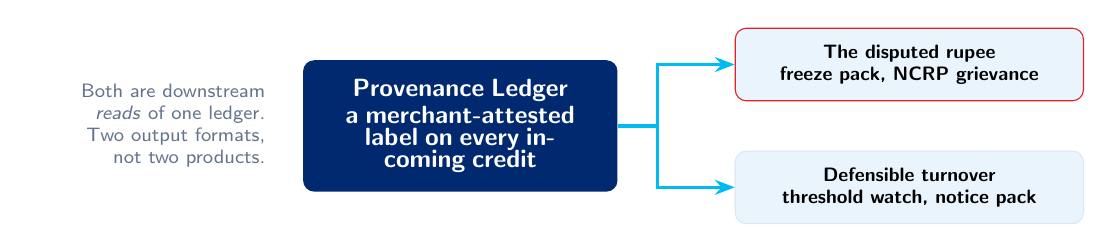
\begin{tikzpicture}[font=\scriptsize]
\node[rounded corners=4pt,fill=navy,text=white,inner sep=7pt,align=center,text width=3.5cm]
  (eng) {\bfseries\small Provenance Ledger\\[0.15em] a merchant-attested label on every incoming credit};
\node[rounded corners=4pt,fill=tint,draw=bad,inner sep=6pt,align=center,text width=4.0cm]
  (tax) at ($(eng.east)+(3.7,0.78)$) {\bfseries The disputed rupee\\ freeze pack, NCRP grievance};
\node[rounded corners=4pt,fill=tint,draw=hairline,inner sep=6pt,align=center,text width=4.0cm]
  (fra) at ($(eng.east)+(3.7,-0.78)$) {\bfseries Defensible turnover\\ threshold watch, notice pack};
\draw[-{Stealth[length=2.5mm]},ptmcyan,line width=1.3pt] (eng.east) -- ++(0.5,0) |- (tax.west);
\draw[-{Stealth[length=2.5mm]},ptmcyan,line width=1.3pt] (eng.east) -- ++(0.5,0) |- (fra.west);
\node[anchor=east,text width=2.9cm,align=right,text=muted] at ($(eng.west)+(-0.35,0)$)
  {Both are downstream \emph{reads} of one ledger. Two output formats, not two products.};
\end{tikzpicture}
\end{center}
\vspace{0.1cm}
\begin{center}
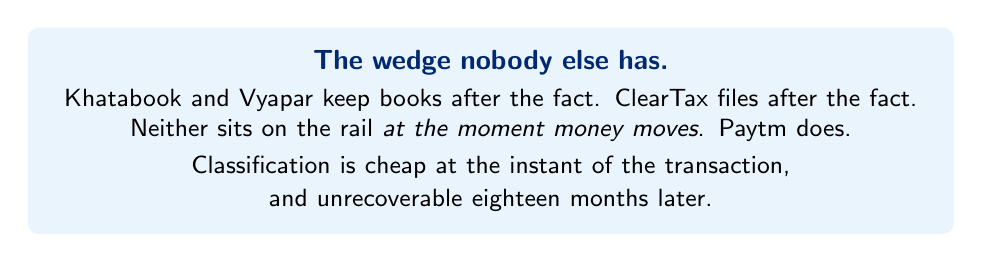
\begin{tikzpicture}\node[rounded corners=4pt,fill=tint,inner sep=8pt,text width=11.2cm,align=center]{
{\bfseries\color{navy}The wedge nobody else has.}\\[0.25em]
\small Khatabook and Vyapar keep books after the fact. ClearTax files after the fact.\\
Neither sits on the rail \emph{at the moment money moves}. Paytm does.\\[0.25em]
\small Classification is cheap at the instant of the transaction,\\ and unrecoverable eighteen months later.
};\end{tikzpicture}
\end{center}
\note{{\color{navy}\bfseries\normalsize 6.~The insight}\par\vspace{0.55em}\textbf{0:40 --- why this is one product, not two.}
\\[0.4em]
Say: \emph{``Most teams would build the fraud tool or the tax tool. They are the
same engine.''} Both are downstream reads of one ledger --- two output formats,
and the freeze pack is the one we lead with.
\\[0.4em]
Then the wedge, and say it slowly because it is the defensible-moat answer:
Khatabook and Vyapar keep books after the fact, ClearTax files after the fact.
Neither sits on the rail at the moment money moves. \textbf{Paytm does.}
\\[0.4em]
Landing line: classification is cheap and accurate at the instant of the
transaction, and unrecoverable eighteen months later when the notice arrives.}
\end{frame}

% ============================================================ 7. THE ENGINE
\begin{frame}{The engine}{Eight tags, one tap}
\vspace{0.15cm}
\begin{columns}[T]
\begin{column}{0.45\textwidth}
{\color{navy}\bfseries\small Every incoming credit gets one tag}\\[0.4em]
{\scriptsize
\begin{tabular}{@{}ll@{}}
\texttt{taxable\_supply}    & ordinary sale \\
\texttt{exempt\_supply}     & vegetables, milk, loose rice \\
\texttt{personal\_transfer} & spouse, parent, sibling \\
\texttt{inter\_account}     & her own money \\
\texttt{refund\_reversal}   & money back from a vendor \\
\texttt{duplicate}          & paid twice, one refunded \\
\texttt{non\_business}      & loan, chit payout, gift \\
{\color{bad}\texttt{unclassified}} & {\color{bad}not enough signal: ask her} \\
\end{tabular}}
\\[0.75em]
{\scriptsize\color{muted}98.6\% are ordinary sales, settled by rules. The agent reasons only about the 1.4\% that need judgement.}
\end{column}
\begin{column}{0.51\textwidth}
\card{6.6cm}{{\bfseries\color{navy}The agent proposes. The merchant attests.}\\[0.4em]
\scriptsize You cannot infer \qm{my husband sent this} from a QR payment. The agent proposes a tag \emph{with its reason}; she confirms with one tap, in Kannada, batched daily.\\[0.45em]
\scriptsize Not a fallback. A ledger she attested \emph{at the time} survives a hearing. An algorithm's guess, made under duress a year later, does not.}
\\[0.55em]
\hspace{0.15cm}\begin{minipage}{6.6cm}
{\bfseries\color{navy}\small Budget: at most 3 questions a day.}\\[0.15em]
{\scriptsize\color{muted}Over a simulated year: \hi{189 questions, median 1.3 a day}. Ask more and the product is dead.}
\end{minipage}
\end{column}
\end{columns}
\note{{\color{navy}\bfseries\normalsize 7.~The engine}\par\vspace{0.55em}\textbf{0:45 --- the mechanism. Do not read the tag list.}
\\[0.4em]
Gesture at the eight tags, say ``eight labels, every incoming credit gets one,''
and move to the right-hand card, which is the real content.
\\[0.4em]
\textbf{The line that matters:} you cannot infer ``my husband sent this'' from a
QR payment. So the agent proposes a tag \emph{with its reason} and she confirms
with one tap. This is not a fallback --- a ledger she attested contemporaneously
survives a hearing; an algorithm's guess produced under duress a year later does not.
\\[0.4em]
Then the budget: at most three questions a day, and we measured 189 across a
year, median 1.3. Ask more than that and the product is dead.
\\[0.4em]
If asked about cost: 98.6\% are ordinary sales settled by rules. The model only
sees the 1.4\% that need judgement.}
\end{frame}

% ============================================================ 8. PRODUCT
\begin{frame}{What the merchant sees}
\vspace{-0.1cm}
\begin{center}
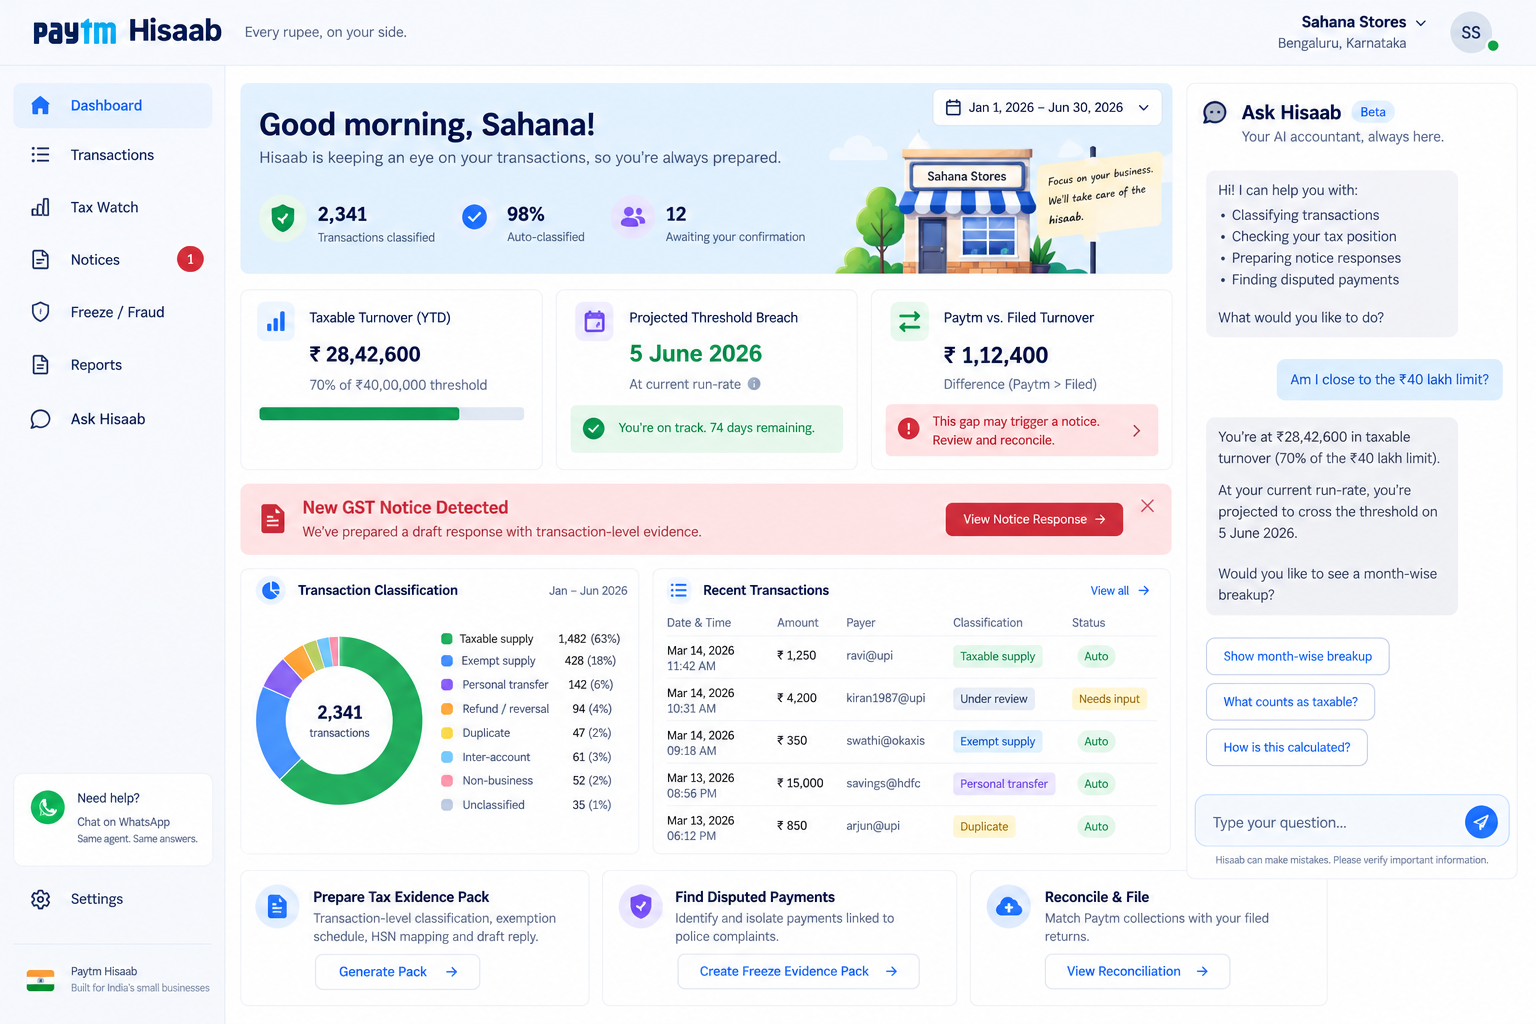
\includegraphics[width=\textwidth,height=0.70\textheight,keepaspectratio]{Paytm-Hisaab_website_look.png}
\end{center}
\vspace{0.1cm}
\hspace{0.05cm}{\scriptsize\color{muted}One surface: what every payment was classified as, how close she is to the threshold, and the packs. The same agent runs on WhatsApp, where she actually is.}
\note{{\color{navy}\bfseries\normalsize 8.~What the merchant sees}\par\vspace{0.55em}\textbf{0:20 --- a glance slide. Do not tour the UI.}
\\[0.4em]
One sentence: everything classified, how close she is to the threshold, and the
packs, on one surface.
\\[0.4em]
Then the WhatsApp point --- the same agent, where she actually is --- and advance.
\\[0.4em]
If someone asks whether this is built: the chat and the tools are live; this
screen is the product surface we are designing toward.}
\end{frame}

% ============================================================ 9. ARCHITECTURE
\begin{frame}{Built on Phinite}{Two agent graphs, four agents, ten deterministic skills}
\vspace{0.15cm}
\begin{columns}[T]
\begin{column}{0.53\textwidth}
{\scriptsize
\begin{tabular}{@{}L{1.75cm}L{4.7cm}@{}}
\multicolumn{2}{@{}l}{\color{navy}\bfseries\small hisaab-watch \;\scriptsize(autonomous: cron + API)}\\
\midrule
Provenance & proposes a tag and a reason for the hard credits \\
Evidence   & assembles packs: freeze evidence, then exemption schedules and HSN \\
\addlinespace[0.6em]
\multicolumn{2}{@{}l}{\color{navy}\bfseries\small hisaab-merchant \;\scriptsize(conversational: chat)}\\
\midrule
Merchant   & the conversation: attestation, alerts, Kannada \\
Escalation & decides when to stop and route to a human CA \\
\bottomrule
\end{tabular}}
\\[0.75em]
{\scriptsize\color{muted}The nightly pass writes its queue to the ledger; the chat reads it when she opens it. Deliberately \emph{not} a graph-to-graph call: a queue that outlives either run is what makes the handoff robust.}
\end{column}
\begin{column}{0.44\textwidth}
\card{5.7cm}{{\bfseries\color{navy}Permissions are the product}\\[0.4em]
\scriptsize Provenance proposes, \red{never commits}.\\[0.25em]
\scriptsize Merchant is the \emph{only} agent that can commit a tag.\\[0.25em]
\scriptsize Evidence is \red{read-only}. It cannot edit a classification to make a pack look better.\\[0.25em]
\scriptsize Escalation can \red{halt} any pack; a human approves.}
\\[0.5em]
\hspace{0.1cm}\begin{minipage}{5.7cm}{\scriptsize\color{muted}Ten tools run live against a hosted service. Every number in a pack traces back, in the trace, to the credit and the attestation behind it.}\end{minipage}
\end{column}
\end{columns}
\note{{\color{navy}\bfseries\normalsize 9.~Built on Phinite}\par\vspace{0.55em}\textbf{0:40 --- for the technical judges.}
\\[0.4em]
Two agent graphs, not four loose agents: \texttt{hisaab-watch} runs autonomously on
cron, \texttt{hisaab-merchant} is the conversation. The nightly pass writes a queue;
the chat reads it when she opens it --- deliberately not a graph-to-graph call,
because a queue that outlives either run is what makes the handoff robust.
\\[0.4em]
\textbf{Spend your time on the right-hand card.} The strongest line in it:
the Evidence agent is read-only --- \emph{the agent that builds the defence cannot
edit the evidence.} And only the Merchant agent can commit an attested tag.
\\[0.4em]
Those are enforced as Phinite tool policies, not conventions, and a denied call
shows up in the trace.}
\end{frame}

% ============================================================ 10. DESIGN DECISIONS
\begin{frame}{Four decisions that make it defensible}
\vspace{0.3cm}
\begin{columns}[T]
\begin{column}{0.48\textwidth}
\card{6.0cm}{{\bfseries\color{navy}1. Arithmetic lives in skills, not the model}\\[0.35em]
\scriptsize Turnover, projections and apportionment are deterministic Python: versioned, testable, traceable. Wrapping arithmetic in an LLM is the standard tell, and the trace would show it.}
\\[0.35em]
\card{6.0cm}{{\bfseries\color{navy}3. Refusing to guess is a feature}\\[0.35em]
\scriptsize An \texttt{unclassified} credit routed to the merchant costs one tap. A confident wrong tag inside an evidence pack is a catastrophe. We report the refusal rate honestly.}
\end{column}
\begin{column}{0.48\textwidth}
\card{6.0cm}{{\bfseries\color{navy}2. Attestation is the promotion boundary}\\[0.35em]
\scriptsize Nothing enters a production pack that the merchant has not confirmed. Sandbox to UAT to prod, with her tap as the gate.}
\\[0.35em]
\card{6.0cm}{{\bfseries\color{navy}4. Ground truth, so accuracy is a number}\\[0.35em]
\scriptsize We simulated a year of a shop's life from a known process, split into what Paytm can see and what really happened. Agents read only the visible half, which is why we quote error bars instead of vibes.}
\end{column}
\end{columns}
\note{{\color{navy}\bfseries\normalsize 10.~Four decisions}\par\vspace{0.55em}\textbf{0:35 --- the slide that separates you from a demo.}
\\[0.4em]
Lead with \#1: all arithmetic is deterministic Python, not model output. Wrapping
arithmetic in an LLM is the standard tell, and the trace would show it.
\\[0.4em]
Then \#3: refusing to guess is a feature. An \texttt{unclassified} credit costs one
tap; a confident wrong tag inside an evidence pack is a catastrophe.
\\[0.4em]
Skim \#2 and \#4 --- one clause each. \#4 is worth a beat if the room is technical:
we generated ground truth, so accuracy is a number instead of a claim.}
\end{frame}

% ============================================================ 11. DEMO / ATTESTATION
\begin{frame}{Demo $\cdot$ Sahana Stores, Jayanagar}{An ordinary Tuesday, before anything goes wrong}
\vspace{0.1cm}
\begin{columns}[T]
\begin{column}{0.48\textwidth}
{\scriptsize\color{muted}Tuesday 10 March. Thirty-nine credits came in over the weekend. The agent asks about \hi{three}.}
\\[0.4em]
\card{5.9cm}{{\kn\scriptsize ಭಾನುವಾರ ರಾತ್ರಿ ₹15,000. ನಿಮ್ಮ ಸ್ವಂತ ಹಣವೇ?}\\[0.25em]
{\color{muted}\scriptsize \qm{₹15,000 at 11:04pm Sunday, from your savings account. Your own money?}}\\[0.35em]
{\scriptsize\color{navy}\fbox{\kn ಹೌದು}\;\fbox{\kn ಇಲ್ಲ}}}
\\[0.4em]
{\scriptsize $\cdot$\; ₹7,500 from her husband, scanned at the shop QR\\[0.25em]
$\cdot$\; ₹4,850 from Raghu Shetty, who has bought twice before. A real sale, and the agent \emph{asks} rather than assumes.}
\\[0.4em]
{\scriptsize\color{muted}The other thirty-six settle silently, and a ₹23 payment nobody can place is left alone.}
\end{column}
\begin{column}{0.48\textwidth}
\ocard{amber}{6.1cm}{{\bfseries\color{amber}And yes, two of those three should not be there}\\[0.35em]
\scriptsize A business QR is not for personal money, and the terms say so. It arrives anyway: family, own top-ups, a chit payout. The rule does not prevent it. It only means \emph{nobody keeps a record of it.}}
\\[0.45em]
{\scriptsize Paytm already reads the signals: channel, linked VPAs, payer history. What no system has is the \hi{merchant's own answer}, given at the time, in her language, and kept.}
\\[0.45em]
{\scriptsize That record is what the next two slides are built from: first for the police, then for the department.}
\end{column}
\end{columns}
\note{{\color{navy}\bfseries\normalsize 11.~Demo --- an ordinary Tuesday (beat 1)}\par\vspace{0.55em}\textbf{0:45 --- or hand over to the live demo here.}
\\[0.4em]
Thirty-nine credits came in over the weekend, the agent asks about \textbf{three}.
Read the Kannada line if you can; otherwise read the gloss under it.
\\[0.4em]
\textbf{Do not hide from the right-hand card --- lead with it.} The mid-review
point was that personal money is not allowed on a business QR. Correct, and we say
so on the slide. The argument is that the rule does not stop it, it only means no
one records it, and an unrecorded credit is what an authority later reads as income.
\\[0.4em]
\textbf{Second half of that card matters just as much.} We are not claiming Paytm
does nothing. It already reads channel, linked VPAs and payer history. What no
system has is her own answer, captured while it is still knowable. That is the
product, and it is a smaller, truer claim than the one we started with.
\\[0.4em]
\textbf{Before going on stage:} confirm the attestation queue is whole ---
\texttt{pending\_total} must be 3. A rehearsal that taps through this beat spends the
queue, and Render needs a clear-cache redeploy to restore it.}
\end{frame}

% ============================================================ 12. DEMO / THE FREEZE
\begin{frame}{Demo $\cdot$ The emergency}{The account is frozen at 09:30 and the supplier payment is due}
\vspace{0.2cm}
\begin{columns}[T]
\begin{column}{0.46\textwidth}
{\scriptsize She sold someone 12kg of onions. That customer was three layers downstream of a fraud victim. She is not named in the FIR, which was filed in another state, and \hi{339 payments} came in that week.}
\\[0.5em]
\card{5.8cm}{{\bfseries\color{navy}The agent isolates it}\\[0.35em]
\scriptsize ₹4,200 on 21 March at 19:47, till POS01. Matched by UTR \emph{and independently} by amount and date.\\[0.3em]
\scriptsize The sale record comes with it: the POS bill, the items, the till and the minute.}
\end{column}
\begin{column}{0.49\textwidth}
\ocard{amber}{6.1cm}{{\bfseries\color{amber}And the decoy it did not choose}\\[0.35em]
\scriptsize A \emph{second} ₹4,200 that same week, from a regular customer. Listed in the pack, and explicitly \emph{not} named as the disputed one. Only the date separates them.}
\\[0.5em]
{\scriptsize Then it drafts the NCRP-CFCFRMS grievance, citing the judgments that only the \emph{disputed amount} should be lien-marked, not the whole account.}
\\[0.5em]
{\scriptsize\color{bad}\bfseries It never asserts that she is innocent.}\\[0.1em]
{\scriptsize\color{muted}Some frozen accounts genuinely are mule accounts. The agent assembles evidence; a human decides. Escalation holds the pack for approval.}
\end{column}
\end{columns}
\note{{\color{navy}\bfseries\normalsize 12.~Demo --- the emergency (beat 4)}\par\vspace{0.55em}\textbf{0:50 --- this is now the lead case. Give it the most time of the three.}
\\[0.4em]
Set the stakes in one sentence: account frozen at half nine, supplier payment due,
339 payments came in that week, and she is not named in the FIR.
\\[0.4em]
\textbf{Why this one leads.} She did nothing wrong and there is no rule she broke.
She sold onions to a customer who turned out to be laundering. Every objection
available against the tax case --- she should not have taken personal money on that
QR, she should have registered --- has no purchase here at all.
\\[0.4em]
The agent isolates ₹4,200 by UTR \emph{and independently} by amount and date, and
brings the POS bill with it --- the items, till POS01, 19:47.
\\[0.4em]
\textbf{The decoy is the point.} A second ₹4,200 that same week from a regular
customer, listed in the pack and explicitly not chosen. Anyone can match an amount;
the pack shows its work.
\\[0.4em]
Finish on the red line: it never asserts she is innocent. Some frozen accounts
genuinely are mule accounts. We assemble evidence; a human decides, and Escalation
holds the pack for approval.}
\end{frame}

% ============================================================ 13. DEMO / TAX
\begin{frame}{Demo $\cdot$ The warning, and the notice}{The same ledger, read for the other authority}
\vspace{0.15cm}
\begin{columns}[T]
\begin{column}{0.38\textwidth}
{\scriptsize\color{muted}Replayed as of 31 January:}
\\[0.35em]
\ocard{good}{4.8cm}{{\bfseries\color{ink}\scriptsize\qm{At your current rate you cross ₹40 lakh around {\color{bad}14 March}. You will need to register.}}\\[0.35em]
{\scriptsize\color{muted}\grn{43 days of warning}, and the date is computed, not typed.}}
\\[0.45em]
{\scriptsize\color{bad}\bfseries This beat is what makes the pitch safe.}\\[0.1em]
{\scriptsize\color{muted}Its first act on the tax side is telling her to register.}
\end{column}
\begin{column}{0.58\textwidth}
{\scriptsize\color{muted}Then the notice arrives, claiming {\color{bad}\bfseries ₹60.98L} of turnover:}
\\[0.3em]
{\scriptsize
\begin{tabular}{@{}lr@{\hskip 1.2em}l@{}}
\multicolumn{2}{@{}l}{\color{navy}\bfseries Aggregate turnover \quad ₹42.2L} & \sub{within \grn{1.6\%} of truth} \\
\midrule
Exempt supplies      & ₹31.3L & \sub{vegetables, loose rice} \\
Taxable supplies     & ₹10.9L & \sub{branded goods, oil, soap} \\
\addlinespace[0.45em]
\multicolumn{2}{@{}l}{\color{navy}\bfseries Not turnover at all \quad ₹18.8L} & \sub{every line traced} \\
\midrule
Her own accounts     & ₹7.4L & \sub{top-ups before supplier runs} \\
Family               & ₹6.1L & \sub{spouse, parent, in-law} \\
Loans, chit, gifts   & ₹4.3L & \sub{chit payout, festival gifts} \\
Refunds, duplicates  & ₹1.0L & \sub{crate returns, double-taps} \\
\bottomrule
\end{tabular}}
\\[0.45em]
{\scriptsize And it says plainly: \hi{the claim is wrong, and you \emph{did} cross ₹40 lakh on 14 March. You must register.}}
\end{column}
\end{columns}
\note{{\color{navy}\bfseries\normalsize 13.~Demo --- the warning and the notice (beats 2 and 3)}\par\vspace{0.55em}\textbf{0:50 --- two tax beats on one slide, deliberately compressed.}
\\[0.4em]
Left: replayed as of 31 January, the agent says she crosses ₹40 lakh around
14 March. \textbf{Say the red line out loud} --- its first act on the tax side is
telling her she owes a registration. That is what stops the room turning hostile.
\\[0.4em]
Right: the notice claims ₹60.98 lakh, and the pack answers it line by line, every
figure traceable to transaction IDs. Then the honest half:
\textbf{the claim is wrong, and she did cross ₹40 lakh, and she must register.}
\\[0.4em]
\textbf{If a judge diffs this against slide 5:} slide 5 shows seeded truth
(₹42.9L), this shows what our system computed (₹42.2L). The 1.6\% between them
\emph{is} the accuracy claim --- say that, do not hedge.
\\[0.4em]
\textbf{If pushed on the personal and own-account lines:} same answer as slide 11.
Those credits should not be on a business QR, they are there anyway, and the
alternative to classifying them is letting them be read as income.}
\end{frame}

% ============================================================ 14. NUMBERS
\begin{frame}{What we can actually prove}{One merchant, one year, 13,267 credits, scored against seeded truth}
\vspace{0.45cm}
\begin{columns}[T]
\begin{column}{0.33\textwidth}
\begin{center}\bignum{1.6\%}{error on aggregate turnover\\ (taxable share within 1\%)}\end{center}
\vspace{0.55cm}
\begin{center}\bignum{43 days}{of warning before the\\ threshold crossing}\end{center}
\end{column}
\begin{column}{0.33\textwidth}
\begin{center}\bignum{1.3 a day}{median questions asked.\\ 189 in a year, never over 3}\end{center}
\vspace{0.55cm}
\begin{center}\bignum{zero}{credits left untagged\\ across the whole year}\end{center}
\end{column}
\begin{column}{0.30\textwidth}
\card{3.8cm}{{\bfseries\color{navy}The honest baseline}\\[0.35em]
\scriptsize A 50-line rules-only classifier gets 99.3\% on sale vs not-a-sale, but catches only \red{77.8\%} of non-sale credits.\\[0.3em]
\scriptsize That residue alone puts two eval merchants on the \emph{wrong side} of ₹40L.\\[0.3em]
\scriptsize Closing it is what the agent plus one tap is for.}
\end{column}
\end{columns}
\vspace{0.45cm}
\hspace{0.1cm}{\scriptsize\color{muted}She corrected the agent 52 times that year. Those corrections are the ledger's strongest evidence, not its failures.}
\note{{\color{navy}\bfseries\normalsize 14.~What we can actually prove}\par\vspace{0.55em}\textbf{0:30 --- do not read all four. Pick two.}
\\[0.4em]
Lead with \textbf{1.6\%} error on turnover and \textbf{1.3 questions a day}. The
other two are there to be read, not narrated.
\\[0.4em]
\textbf{The credibility move is the box on the right} --- volunteer the weakness
before anyone finds it. A rules-only baseline gets 99.3\% on sale vs not-a-sale
but catches only 77.8\% of non-sale credits, and that residue alone puts two eval
merchants on the wrong side of ₹40 lakh. Closing it is what the agent plus one tap is for.
\\[0.4em]
Last line if you have the beat: she corrected the agent 52 times that year, and
those corrections are the ledger's strongest evidence, not its failures.}
\end{frame}

% ============================================================ 15. CLOSE
\begin{frame}{The line we do not cross}{Accuracy, not minimisation}
\vspace{0.3cm}
\begin{columns}[T]
\begin{column}{0.52\textwidth}
{\scriptsize
$\cdot$\; We \hi{never assert innocence} on a freeze. Some accounts really are mule accounts. We assemble evidence; a human decides.\\[0.5em]
$\cdot$\; We \hi{file nothing} with any authority. Artefacts only; the merchant or their CA files.\\[0.5em]
$\cdot$\; We compute what she \hi{genuinely owes} and say so plainly, including \qm{you crossed the threshold, you must register.}\\[0.5em]
$\cdot$\; We \hi{never assert a final liability}. We compute, show the workings, and route to a CA.\\[0.5em]
$\cdot$\; A business QR is \hi{not for personal money}. We do not excuse it. We record it, so it is not read as income.}
\end{column}
\begin{column}{0.44\textwidth}
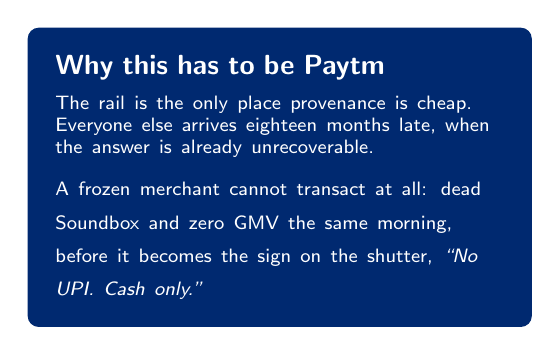
\begin{tikzpicture}\node[rounded corners=4pt,fill=navy,text=white,inner sep=10pt,text width=5.7cm,align=left]{
{\bfseries Why this has to be Paytm}\\[0.45em]
\scriptsize The rail is the only place provenance is cheap. Everyone else arrives eighteen months late, when the answer is already unrecoverable.\\[0.45em]
\scriptsize A frozen merchant cannot transact at all: dead Soundbox and zero GMV the same morning, before it becomes the sign on the shutter, \emph{\qm{No UPI. Cash only.}}
};\end{tikzpicture}
\end{column}
\end{columns}
\vspace{0.4cm}
\begin{center}
{\large\color{navy}\bfseries Paytm Hisaab}\quad{\color{muted}every rupee, on your side.}
\end{center}
\note{{\color{navy}\bfseries\normalsize 15.~The line we do not cross}\par\vspace{0.55em}\textbf{0:30 --- the non-negotiables, fast, then land.}
\\[0.4em]
Run the five bullets at pace. The one to hit is the first: we never assert
innocence on a freeze. The last is the mid-review answer, on the slide on purpose.
\\[0.4em]
Then the navy box: provenance is cheap only on the rail, and a frozen merchant
stops transacting the same morning.
\\[0.4em]
Final line, unhurried: \emph{``Paytm Hisaab. Every rupee, on your side.''} Stop talking.
\\[0.5em]
{\scriptsize
{\color{navy}\bfseries --- Q\&A prep ---}
\\[0.3em]
\textbf{``Merchants may not take personal money on a business QR.''} Correct, and
slide 11 says so before you have to. It arrives anyway, and the alternative to
recording it is letting an authority read it as income. We are not defending the
behaviour --- we are refusing to let it become a liability.
\\[0.3em]
\textbf{``Paytm already tags transactions.''} It does, and we build on that rather
than around it: channel, linked VPAs and payer history feed the rules layer. What
no tag carries is her attestation --- the part an authority accepts, and the only
part she alone can give.
\\[0.3em]
\textbf{``No return mismatch?''} That check needs a \emph{registered} composition
dealer who filed a CMP-08 to disagree with. Ours is unregistered, which is why she
gets a notice at all; the eval split has one with four quarters seeded.
\\[0.3em]
\textbf{``Exempt vs taxable on a QR sale?''} Not per payment. We apportion by value
from that shop's own POS-billed ratio and label it an estimate. Labelling each sale
by its majority side understated taxable turnover threefold.
\\[0.3em]
\textbf{``Four LLM calls in a trenchcoat?''} Everything deterministic is a skill and
four agents is the ceiling. If twenty lines of Python replaces an agent, it should
have been a skill --- the trace shows which is which.
\\[0.3em]
\textbf{``No standing with the police.''} Agreed: Paytm supplies, the merchant
files. By design. Cash sales are real, out of scope, and on the slide.}}
\end{frame}

\end{document}
"
\ifdefined\shownotes
  \setbeamertemplate{note page}{%
    \usebeamercolor[fg]{normal text}%
    \vspace{0.2em}%
    {\scriptsize\color{muted}Paytm Hisaab \;$\cdot$\; speaker notes}\hfill
    {\scriptsize\color{muted}slide \insertframenumber\ of 15}\par
    \vspace{0.25em}{\color{ptmcyan}\rule{\textwidth}{1.5pt}}\par
    \vspace{0.55em}\footnotesize\raggedright\insertnote\par}
  \setbeameroption{show only notes}
\fi

\begin{document}

% ============================================================ 1. TITLE
{\setbeamertemplate{footline}{}
\begin{frame}[plain]
\vspace{0.9cm}
\begin{center}
{\fontsize{38}{42}\selectfont\bfseries\color{navy}Paytm\;\color{ink}Hisaab}\\[0.45em]
{\Large\color{muted}Every rupee, on your side.}\\[0.9em]
{\color{ptmcyan}\rule{2.8cm}{2.5pt}}\\[0.9em]
{\large\color{ink}The agent that lets a merchant account for their own money}\\[0.15em]
{\large\color{ink}when someone in authority demands an explanation.}\\[1.3em]
{\small\color{muted}Agent Labs Buildathon \;$\cdot$\; Phinite $\times$ Paytm \;$\cdot$\; Track 2: AI for Small Businesses}
\end{center}
\note{{\color{navy}\bfseries\normalsize 1.~Title}\par\vspace{0.55em}\textbf{0:10 --- open cold.} Do not read the title or the tagline off the slide.
\\[0.4em]
Say: \emph{``I want to tell you about a man in Haveri who opened an envelope.''} Then advance.
\\[0.4em]
Nothing on this slide needs explaining. The tagline lands at the end, not here.}
\end{frame}}

% ============================================================ 2. STORY
\begin{frame}{Haveri, 2025}{A vegetable vendor opens an envelope}
\vspace{0.05cm}
\begin{columns}[T]
\begin{column}{0.52\textwidth}
\vspace{0.15cm}
He sells vegetables. Vegetables are \hi{exempt} from GST.\\[0.6em]
He also took UPI, because Paytm asked him to.\\[0.6em]
Four years of credits into his account, added up and billed as income:
\begin{center}\vspace{0.1em}{\fontsize{30}{32}\selectfont\bfseries\color{bad}₹29 lakh}\end{center}
\end{column}
\begin{column}{0.44\textwidth}
\ocard{hairline}{5.4cm}{\centering
  {\color{muted}\scriptsize Within weeks, on shutters across Karnataka:}\\[0.6em]
  {\fontsize{20}{23}\selectfont\bfseries\color{ink}\qm{No UPI.\\ Cash only.}}\\[0.6em]
  {\color{muted}\scriptsize A statewide boycott, by the merchants who had just adopted it.}}
\end{column}
\end{columns}
\vspace{0.25cm}
\hspace{0.1cm}{\small\sub{Withdrawn for the traders who could \emph{show} what they sold. Most could not. And tax is no longer the only authority asking.}}
\note{{\color{navy}\bfseries\normalsize 2.~Haveri, 2025}\par\vspace{0.55em}\textbf{0:45 --- the hook. Tell it, do not summarise it.}
\\[0.4em]
Four beats, in this order: he sells vegetables; vegetables are exempt from GST;
he took UPI because \emph{we} asked him to; the department added up four years of
credits and sent him a bill for \textbf{₹29 lakh}.
\\[0.4em]
\textbf{Pause on the number.} Then the card: within weeks, shutters across Karnataka
read ``No UPI, cash only.'' Merchants we had just onboarded, boycotting the rail.
\\[0.4em]
Close on the bottom line --- the notices were withdrawn for traders who could
\emph{show} what they sold. Most could not. That verb is the whole product.
\\[0.4em]
\textbf{Then the bridge:} \emph{``and tax is no longer the only authority asking.''}
That sentence is doing the repositioning --- Haveri is not a tax story here, it is
the moment taking digital money became a liability. The sharper version of it is
two slides away.
\\[0.4em]
\textbf{Do not say this is happening right now.} It is 2025. The next slide is
what makes it current, and a judge who knows the episode will respect the distinction.}
\end{frame}

% ============================================================ 3. STILL HAPPENING
\begin{frame}{And this is not a 2025 story}{CAclubindia, last updated 02 September 2026: ten days ago}
\vspace{0.1cm}
\begin{center}

\includegraphics[width=12.4cm]{gst-notices-2026.png}
\end{center}
\vspace{0.35cm}
\card{13.1cm}{\scriptsize\qm{During August 2026, the GST Department issued a significant number of notices covering different financial years and involving a wide range of issues\ldots\ They covered matters such as ITC mismatches, ineligible credit, \hi{differences in turnover}, wrong GST classification or rate, \hi{exemption claims}, Reverse Charge Mechanism\ldots}}
\vspace{0.3cm}

\hspace{0.1cm}{\small Those two categories are the whole content of an evidence pack. And this is the \emph{slower} of the two authorities. The other one freezes the account first.}
\note{{\color{navy}\bfseries\normalsize 3.~And this is not a 2025 story}\par\vspace{0.55em}\textbf{0:25 --- fast. This slide exists to kill one objection.}
\\[0.4em]
Say: \emph{``That was last year. This was published ten days ago.''}
\\[0.4em]
Do not read the quote. Point at the two bolded phrases only ---
\textbf{differences in turnover} and \textbf{exemption claims} --- and say those
two categories are the entire content of what we build.
\\[0.4em]
\textbf{Land on the last line and move.} It is the handoff into the police
slide: this is the slower authority. The other one freezes first and asks
afterwards. Do not linger here --- tax is no longer the headline.}
\end{frame}

% ============================================================ 4. THE TRAP
\begin{frame}{Every rupee a merchant receives is now evidence}{Today it is only ever used against them}
\vspace{0.05cm}
\begin{columns}[T]
\begin{column}{0.47\textwidth}
\ocard{bad}{6.0cm}{{\bfseries\color{bad}The cyber-crime police}\\[0.35em]
\scriptsize Fraud money layers through accounts within minutes. The shop at the end of the chain, the one that sold someone a watermelon, is frozen. It did nothing wrong, is not named in the FIR, and finds out when a payment declines.}
\end{column}
\begin{column}{0.47\textwidth}
\card{6.1cm}{{\bfseries\color{navy}The tax department}\\[0.35em]
\scriptsize Compares UPI collections against filed returns and bills the difference. Registered traders too, with QR, wallet, card and cash deposits all in scope.}
\end{column}
\end{columns}
\vspace{0.4cm}
\begin{center}
{\large Both demand the same artefact: \hi{what was each rupee, actually?}}\\[0.3em]
{\small\color{muted}Paytm already sees more of this than anyone. What is missing is the \emph{merchant's own answer}, captured when it is still knowable.}
\end{center}
\vspace{0.15cm}
{\color{hairline}\hrule height 1pt}
\vspace{0.35em}
\hspace{0.05cm}{\scriptsize\bfseries\color{bad}What it costs Paytm:}~{\scriptsize a frozen merchant stops transacting that morning. A frightened one takes the QR down for good. Dead Soundbox, zero GMV, no lending origination.}
\note{{\color{navy}\bfseries\normalsize 4.~Every rupee is now evidence}\par\vspace{0.55em}\textbf{0:40 --- two authorities, one unanswerable question.}
\\[0.4em]
\textbf{Left card first and give it the time.} Fraud money layers within minutes,
and the shop at the end of the chain, \emph{the one that sold someone a watermelon},
gets frozen. It did nothing wrong, it is not named in the FIR, and it finds out
when a payment declines. Use the watermelon.
\\[0.4em]
Right card briskly: the department reconciles collections against filed returns
and bills the difference. One sentence, then move.
\\[0.4em]
Then the pivot: both demand the same artefact --- what was each rupee, actually.
\\[0.4em]
\textbf{Say the grey line as written.} We do \emph{not} claim Paytm does nothing
with this data --- it tags plenty. The gap is the merchant's own answer, captured
when it is still knowable. Claiming otherwise in this room gets corrected.
\\[0.4em]
\textbf{Slow down for the red line.} This is the business case, not a footnote:
a frozen merchant stops transacting that morning, a frightened one takes the QR
down for good. Dead Soundbox, zero GMV, no lending origination.}
\end{frame}

% ============================================================ 5. THE BAR
\begin{frame}{Gross credits are not turnover}{One shop, one year, ₹60.98 lakh of credits}
\vspace{0.1cm}
\begin{center}
\begin{tikzpicture}[x=1cm,y=1cm]
% --- what the notice counts
\node[anchor=west,font=\scriptsize\bfseries,text=bad] at (-0.05,1.80) {WHAT THE NOTICE COUNTS AS TURNOVER};
\fill[bad!85,rounded corners=2pt] (0,1.06) rectangle (11.4,1.60);
\node[font=\small\bfseries,text=white] at (5.7,1.33) {₹60.98 lakh};

% --- what actually happened   (1 lakh = 0.18696 cm, so the bars are the same length)
\node[anchor=west,font=\scriptsize\bfseries,text=navy] at (-0.05,0.66) {WHAT ACTUALLY HAPPENED};
\fill[good!80,rounded corners=2pt]  (0,-0.08)     rectangle (6.001,0.46);
\fill[good!45]                      (6.001,-0.08) rectangle (8.002,0.46);
\fill[ptmcyan!70]                   (8.002,-0.08) rectangle (9.385,0.46);
\fill[navy!55]                      (9.385,-0.08) rectangle (10.451,0.46);
\fill[amber!70]                     (10.451,-0.08)rectangle (11.255,0.46);
\fill[muted!60,rounded corners=2pt] (11.255,-0.08)rectangle (11.4,0.46);

% brackets
\draw[navy,line width=0.8pt] (0,-0.22) -- (0,-0.36) -- (8.002,-0.36) -- (8.002,-0.22);
\node[anchor=north,font=\scriptsize,text=navy,align=center] at (4.0,-0.38)
  {\bfseries ₹42.9L aggregate turnover\quad{\color{muted}\scriptsize exempt ₹32.1L + taxable ₹10.7L}};
\draw[bad,line width=0.8pt] (8.002,-0.22) -- (8.002,-0.36) -- (11.4,-0.36) -- (11.4,-0.22);
\node[anchor=north,font=\scriptsize,text=bad,align=center] at (9.7,-0.38)
  {\bfseries ₹18.1L that is not turnover at all};

% legend
\node[font=\scriptsize,text=ink] at (5.7,-1.02) {%
\textcolor{good!80}{$\blacksquare$}~Exempt sales \quad
\textcolor{good!45}{$\blacksquare$}~Taxable sales \quad
\textcolor{ptmcyan!70}{$\blacksquare$}~Her own accounts ₹7.4L};
\node[font=\scriptsize,text=ink] at (5.7,-1.40) {%
\textcolor{navy!55}{$\blacksquare$}~Family ₹5.7L \quad
\textcolor{amber!70}{$\blacksquare$}~Loans, chit, gifts ₹4.3L \quad
\textcolor{muted!60}{$\blacksquare$}~Refunds \& duplicates ₹0.7L};
\end{tikzpicture}
\end{center}
\vspace{0.15cm}
\hspace{0.1cm}{\small\sub{Personal money does not belong on a business QR. It arrives anyway, reads as turnover, and hides the one credit the police will ask about.}}
\note{{\color{navy}\bfseries\normalsize 5.~Gross credits are not turnover}\par\vspace{0.55em}\textbf{0:45 --- the hinge of the pitch. Let the picture work.}
\\[0.4em]
Say: \emph{``One shop, one year, ₹60.98 lakh of credits. The red bar is what the
notice counts as turnover --- all of it.''}
\\[0.4em]
Then the bottom bar. \textbf{Stop talking for two seconds} and let them read it.
\\[0.4em]
₹42.9L really is turnover, and we say so. ₹18.1L is not: her savings account, her
husband, a chit payout, a double-tap on the Soundbox.
\\[0.4em]
\textbf{Get in front of the obvious objection.} Personal money is not supposed to
touch a business QR. Say so first, then say it arrives anyway --- that is an
observation about merchants, not a loophole we are selling. The rule does not stop
it; it only means no one is keeping a record of it.
\\[0.4em]
\textbf{And close on the second use.} This volume is also why she cannot find the
one credit the police care about. Same bar, same problem, and the freeze slide
pays it off.
\\[0.4em]
If challenged on the numbers: seeded ground truth from our generator, not an
estimate. Accuracy against it is slide 14.}
\end{frame}

% ============================================================ 6. INSIGHT
\begin{frame}{The insight}{Most teams would build the tax tool \emph{or} the fraud tool. They are the same engine.}
\vspace{0.15cm}
\begin{center}
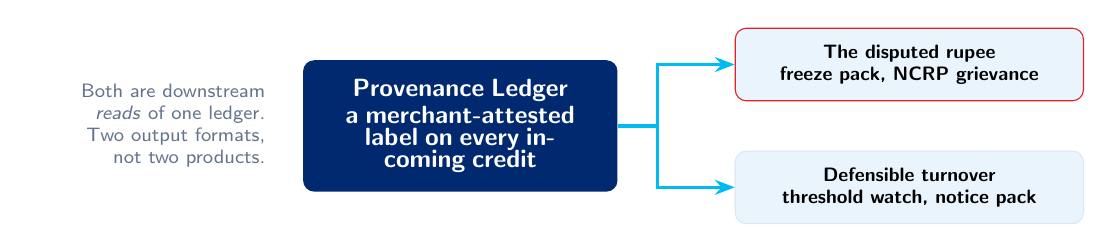
\begin{tikzpicture}[font=\scriptsize]
\node[rounded corners=4pt,fill=navy,text=white,inner sep=7pt,align=center,text width=3.5cm]
  (eng) {\bfseries\small Provenance Ledger\\[0.15em] a merchant-attested label on every incoming credit};
\node[rounded corners=4pt,fill=tint,draw=bad,inner sep=6pt,align=center,text width=4.0cm]
  (tax) at ($(eng.east)+(3.7,0.78)$) {\bfseries The disputed rupee\\ freeze pack, NCRP grievance};
\node[rounded corners=4pt,fill=tint,draw=hairline,inner sep=6pt,align=center,text width=4.0cm]
  (fra) at ($(eng.east)+(3.7,-0.78)$) {\bfseries Defensible turnover\\ threshold watch, notice pack};
\draw[-{Stealth[length=2.5mm]},ptmcyan,line width=1.3pt] (eng.east) -- ++(0.5,0) |- (tax.west);
\draw[-{Stealth[length=2.5mm]},ptmcyan,line width=1.3pt] (eng.east) -- ++(0.5,0) |- (fra.west);
\node[anchor=east,text width=2.9cm,align=right,text=muted] at ($(eng.west)+(-0.35,0)$)
  {Both are downstream \emph{reads} of one ledger. Two output formats, not two products.};
\end{tikzpicture}
\end{center}
\vspace{0.1cm}
\begin{center}
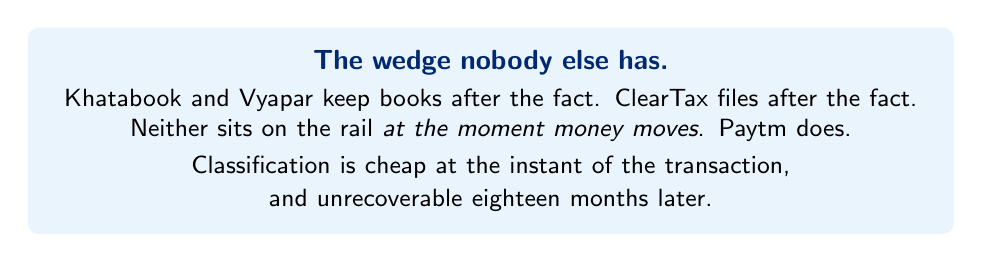
\begin{tikzpicture}\node[rounded corners=4pt,fill=tint,inner sep=8pt,text width=11.2cm,align=center]{
{\bfseries\color{navy}The wedge nobody else has.}\\[0.25em]
\small Khatabook and Vyapar keep books after the fact. ClearTax files after the fact.\\
Neither sits on the rail \emph{at the moment money moves}. Paytm does.\\[0.25em]
\small Classification is cheap at the instant of the transaction,\\ and unrecoverable eighteen months later.
};\end{tikzpicture}
\end{center}
\note{{\color{navy}\bfseries\normalsize 6.~The insight}\par\vspace{0.55em}\textbf{0:40 --- why this is one product, not two.}
\\[0.4em]
Say: \emph{``Most teams would build the fraud tool or the tax tool. They are the
same engine.''} Both are downstream reads of one ledger --- two output formats,
and the freeze pack is the one we lead with.
\\[0.4em]
Then the wedge, and say it slowly because it is the defensible-moat answer:
Khatabook and Vyapar keep books after the fact, ClearTax files after the fact.
Neither sits on the rail at the moment money moves. \textbf{Paytm does.}
\\[0.4em]
Landing line: classification is cheap and accurate at the instant of the
transaction, and unrecoverable eighteen months later when the notice arrives.}
\end{frame}

% ============================================================ 7. THE ENGINE
\begin{frame}{The engine}{Eight tags, one tap}
\vspace{0.15cm}
\begin{columns}[T]
\begin{column}{0.45\textwidth}
{\color{navy}\bfseries\small Every incoming credit gets one tag}\\[0.4em]
{\scriptsize
\begin{tabular}{@{}ll@{}}
\texttt{taxable\_supply}    & ordinary sale \\
\texttt{exempt\_supply}     & vegetables, milk, loose rice \\
\texttt{personal\_transfer} & spouse, parent, sibling \\
\texttt{inter\_account}     & her own money \\
\texttt{refund\_reversal}   & money back from a vendor \\
\texttt{duplicate}          & paid twice, one refunded \\
\texttt{non\_business}      & loan, chit payout, gift \\
{\color{bad}\texttt{unclassified}} & {\color{bad}not enough signal: ask her} \\
\end{tabular}}
\\[0.75em]
{\scriptsize\color{muted}98.6\% are ordinary sales, settled by rules. The agent reasons only about the 1.4\% that need judgement.}
\end{column}
\begin{column}{0.51\textwidth}
\card{6.6cm}{{\bfseries\color{navy}The agent proposes. The merchant attests.}\\[0.4em]
\scriptsize You cannot infer \qm{my husband sent this} from a QR payment. The agent proposes a tag \emph{with its reason}; she confirms with one tap, in Kannada, batched daily.\\[0.45em]
\scriptsize Not a fallback. A ledger she attested \emph{at the time} survives a hearing. An algorithm's guess, made under duress a year later, does not.}
\\[0.55em]
\hspace{0.15cm}\begin{minipage}{6.6cm}
{\bfseries\color{navy}\small Budget: at most 3 questions a day.}\\[0.15em]
{\scriptsize\color{muted}Over a simulated year: \hi{189 questions, median 1.3 a day}. Ask more and the product is dead.}
\end{minipage}
\end{column}
\end{columns}
\note{{\color{navy}\bfseries\normalsize 7.~The engine}\par\vspace{0.55em}\textbf{0:45 --- the mechanism. Do not read the tag list.}
\\[0.4em]
Gesture at the eight tags, say ``eight labels, every incoming credit gets one,''
and move to the right-hand card, which is the real content.
\\[0.4em]
\textbf{The line that matters:} you cannot infer ``my husband sent this'' from a
QR payment. So the agent proposes a tag \emph{with its reason} and she confirms
with one tap. This is not a fallback --- a ledger she attested contemporaneously
survives a hearing; an algorithm's guess produced under duress a year later does not.
\\[0.4em]
Then the budget: at most three questions a day, and we measured 189 across a
year, median 1.3. Ask more than that and the product is dead.
\\[0.4em]
If asked about cost: 98.6\% are ordinary sales settled by rules. The model only
sees the 1.4\% that need judgement.}
\end{frame}

% ============================================================ 8. PRODUCT
\begin{frame}{What the merchant sees}
\vspace{-0.1cm}
\begin{center}
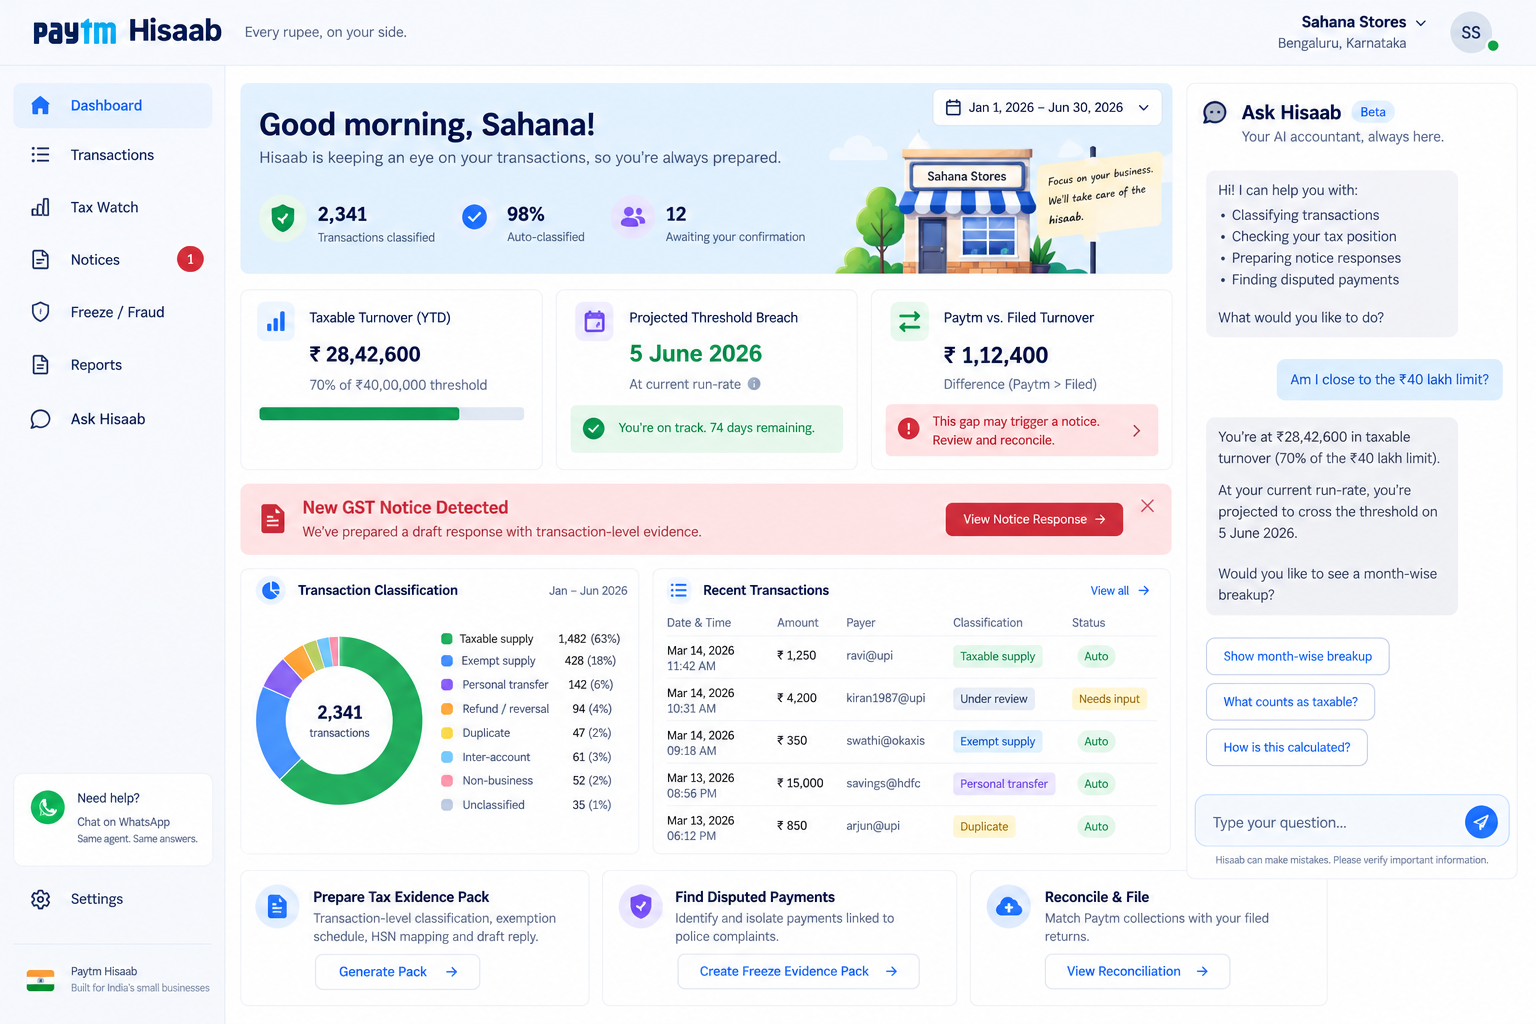
\includegraphics[width=\textwidth,height=0.70\textheight,keepaspectratio]{Paytm-Hisaab_website_look.png}
\end{center}
\vspace{0.1cm}
\hspace{0.05cm}{\scriptsize\color{muted}One surface: what every payment was classified as, how close she is to the threshold, and the packs. The same agent runs on WhatsApp, where she actually is.}
\note{{\color{navy}\bfseries\normalsize 8.~What the merchant sees}\par\vspace{0.55em}\textbf{0:20 --- a glance slide. Do not tour the UI.}
\\[0.4em]
One sentence: everything classified, how close she is to the threshold, and the
packs, on one surface.
\\[0.4em]
Then the WhatsApp point --- the same agent, where she actually is --- and advance.
\\[0.4em]
If someone asks whether this is built: the chat and the tools are live; this
screen is the product surface we are designing toward.}
\end{frame}

% ============================================================ 9. ARCHITECTURE
\begin{frame}{Built on Phinite}{Two agent graphs, four agents, ten deterministic skills}
\vspace{0.15cm}
\begin{columns}[T]
\begin{column}{0.53\textwidth}
{\scriptsize
\begin{tabular}{@{}L{1.75cm}L{4.7cm}@{}}
\multicolumn{2}{@{}l}{\color{navy}\bfseries\small hisaab-watch \;\scriptsize(autonomous: cron + API)}\\
\midrule
Provenance & proposes a tag and a reason for the hard credits \\
Evidence   & assembles packs: freeze evidence, then exemption schedules and HSN \\
\addlinespace[0.6em]
\multicolumn{2}{@{}l}{\color{navy}\bfseries\small hisaab-merchant \;\scriptsize(conversational: chat)}\\
\midrule
Merchant   & the conversation: attestation, alerts, Kannada \\
Escalation & decides when to stop and route to a human CA \\
\bottomrule
\end{tabular}}
\\[0.75em]
{\scriptsize\color{muted}The nightly pass writes its queue to the ledger; the chat reads it when she opens it. Deliberately \emph{not} a graph-to-graph call: a queue that outlives either run is what makes the handoff robust.}
\end{column}
\begin{column}{0.44\textwidth}
\card{5.7cm}{{\bfseries\color{navy}Permissions are the product}\\[0.4em]
\scriptsize Provenance proposes, \red{never commits}.\\[0.25em]
\scriptsize Merchant is the \emph{only} agent that can commit a tag.\\[0.25em]
\scriptsize Evidence is \red{read-only}. It cannot edit a classification to make a pack look better.\\[0.25em]
\scriptsize Escalation can \red{halt} any pack; a human approves.}
\\[0.5em]
\hspace{0.1cm}\begin{minipage}{5.7cm}{\scriptsize\color{muted}Ten tools run live against a hosted service. Every number in a pack traces back, in the trace, to the credit and the attestation behind it.}\end{minipage}
\end{column}
\end{columns}
\note{{\color{navy}\bfseries\normalsize 9.~Built on Phinite}\par\vspace{0.55em}\textbf{0:40 --- for the technical judges.}
\\[0.4em]
Two agent graphs, not four loose agents: \texttt{hisaab-watch} runs autonomously on
cron, \texttt{hisaab-merchant} is the conversation. The nightly pass writes a queue;
the chat reads it when she opens it --- deliberately not a graph-to-graph call,
because a queue that outlives either run is what makes the handoff robust.
\\[0.4em]
\textbf{Spend your time on the right-hand card.} The strongest line in it:
the Evidence agent is read-only --- \emph{the agent that builds the defence cannot
edit the evidence.} And only the Merchant agent can commit an attested tag.
\\[0.4em]
Those are enforced as Phinite tool policies, not conventions, and a denied call
shows up in the trace.}
\end{frame}

% ============================================================ 10. DESIGN DECISIONS
\begin{frame}{Four decisions that make it defensible}
\vspace{0.3cm}
\begin{columns}[T]
\begin{column}{0.48\textwidth}
\card{6.0cm}{{\bfseries\color{navy}1. Arithmetic lives in skills, not the model}\\[0.35em]
\scriptsize Turnover, projections and apportionment are deterministic Python: versioned, testable, traceable. Wrapping arithmetic in an LLM is the standard tell, and the trace would show it.}
\\[0.35em]
\card{6.0cm}{{\bfseries\color{navy}3. Refusing to guess is a feature}\\[0.35em]
\scriptsize An \texttt{unclassified} credit routed to the merchant costs one tap. A confident wrong tag inside an evidence pack is a catastrophe. We report the refusal rate honestly.}
\end{column}
\begin{column}{0.48\textwidth}
\card{6.0cm}{{\bfseries\color{navy}2. Attestation is the promotion boundary}\\[0.35em]
\scriptsize Nothing enters a production pack that the merchant has not confirmed. Sandbox to UAT to prod, with her tap as the gate.}
\\[0.35em]
\card{6.0cm}{{\bfseries\color{navy}4. Ground truth, so accuracy is a number}\\[0.35em]
\scriptsize We simulated a year of a shop's life from a known process, split into what Paytm can see and what really happened. Agents read only the visible half, which is why we quote error bars instead of vibes.}
\end{column}
\end{columns}
\note{{\color{navy}\bfseries\normalsize 10.~Four decisions}\par\vspace{0.55em}\textbf{0:35 --- the slide that separates you from a demo.}
\\[0.4em]
Lead with \#1: all arithmetic is deterministic Python, not model output. Wrapping
arithmetic in an LLM is the standard tell, and the trace would show it.
\\[0.4em]
Then \#3: refusing to guess is a feature. An \texttt{unclassified} credit costs one
tap; a confident wrong tag inside an evidence pack is a catastrophe.
\\[0.4em]
Skim \#2 and \#4 --- one clause each. \#4 is worth a beat if the room is technical:
we generated ground truth, so accuracy is a number instead of a claim.}
\end{frame}

% ============================================================ 11. DEMO / ATTESTATION
\begin{frame}{Demo $\cdot$ Sahana Stores, Jayanagar}{An ordinary Tuesday, before anything goes wrong}
\vspace{0.1cm}
\begin{columns}[T]
\begin{column}{0.48\textwidth}
{\scriptsize\color{muted}Tuesday 10 March. Thirty-nine credits came in over the weekend. The agent asks about \hi{three}.}
\\[0.4em]
\card{5.9cm}{{\kn\scriptsize ಭಾನುವಾರ ರಾತ್ರಿ ₹15,000. ನಿಮ್ಮ ಸ್ವಂತ ಹಣವೇ?}\\[0.25em]
{\color{muted}\scriptsize \qm{₹15,000 at 11:04pm Sunday, from your savings account. Your own money?}}\\[0.35em]
{\scriptsize\color{navy}\fbox{\kn ಹೌದು}\;\fbox{\kn ಇಲ್ಲ}}}
\\[0.4em]
{\scriptsize $\cdot$\; ₹7,500 from her husband, scanned at the shop QR\\[0.25em]
$\cdot$\; ₹4,850 from Raghu Shetty, who has bought twice before. A real sale, and the agent \emph{asks} rather than assumes.}
\\[0.4em]
{\scriptsize\color{muted}The other thirty-six settle silently, and a ₹23 payment nobody can place is left alone.}
\end{column}
\begin{column}{0.48\textwidth}
\ocard{amber}{6.1cm}{{\bfseries\color{amber}And yes, two of those three should not be there}\\[0.35em]
\scriptsize A business QR is not for personal money, and the terms say so. It arrives anyway: family, own top-ups, a chit payout. The rule does not prevent it. It only means \emph{nobody keeps a record of it.}}
\\[0.45em]
{\scriptsize Paytm already reads the signals: channel, linked VPAs, payer history. What no system has is the \hi{merchant's own answer}, given at the time, in her language, and kept.}
\\[0.45em]
{\scriptsize That record is what the next two slides are built from: first for the police, then for the department.}
\end{column}
\end{columns}
\note{{\color{navy}\bfseries\normalsize 11.~Demo --- an ordinary Tuesday (beat 1)}\par\vspace{0.55em}\textbf{0:45 --- or hand over to the live demo here.}
\\[0.4em]
Thirty-nine credits came in over the weekend, the agent asks about \textbf{three}.
Read the Kannada line if you can; otherwise read the gloss under it.
\\[0.4em]
\textbf{Do not hide from the right-hand card --- lead with it.} The mid-review
point was that personal money is not allowed on a business QR. Correct, and we say
so on the slide. The argument is that the rule does not stop it, it only means no
one records it, and an unrecorded credit is what an authority later reads as income.
\\[0.4em]
\textbf{Second half of that card matters just as much.} We are not claiming Paytm
does nothing. It already reads channel, linked VPAs and payer history. What no
system has is her own answer, captured while it is still knowable. That is the
product, and it is a smaller, truer claim than the one we started with.
\\[0.4em]
\textbf{Before going on stage:} confirm the attestation queue is whole ---
\texttt{pending\_total} must be 3. A rehearsal that taps through this beat spends the
queue, and Render needs a clear-cache redeploy to restore it.}
\end{frame}

% ============================================================ 12. DEMO / THE FREEZE
\begin{frame}{Demo $\cdot$ The emergency}{The account is frozen at 09:30 and the supplier payment is due}
\vspace{0.2cm}
\begin{columns}[T]
\begin{column}{0.46\textwidth}
{\scriptsize She sold someone 12kg of onions. That customer was three layers downstream of a fraud victim. She is not named in the FIR, which was filed in another state, and \hi{339 payments} came in that week.}
\\[0.5em]
\card{5.8cm}{{\bfseries\color{navy}The agent isolates it}\\[0.35em]
\scriptsize ₹4,200 on 21 March at 19:47, till POS01. Matched by UTR \emph{and independently} by amount and date.\\[0.3em]
\scriptsize The sale record comes with it: the POS bill, the items, the till and the minute.}
\end{column}
\begin{column}{0.49\textwidth}
\ocard{amber}{6.1cm}{{\bfseries\color{amber}And the decoy it did not choose}\\[0.35em]
\scriptsize A \emph{second} ₹4,200 that same week, from a regular customer. Listed in the pack, and explicitly \emph{not} named as the disputed one. Only the date separates them.}
\\[0.5em]
{\scriptsize Then it drafts the NCRP-CFCFRMS grievance, citing the judgments that only the \emph{disputed amount} should be lien-marked, not the whole account.}
\\[0.5em]
{\scriptsize\color{bad}\bfseries It never asserts that she is innocent.}\\[0.1em]
{\scriptsize\color{muted}Some frozen accounts genuinely are mule accounts. The agent assembles evidence; a human decides. Escalation holds the pack for approval.}
\end{column}
\end{columns}
\note{{\color{navy}\bfseries\normalsize 12.~Demo --- the emergency (beat 4)}\par\vspace{0.55em}\textbf{0:50 --- this is now the lead case. Give it the most time of the three.}
\\[0.4em]
Set the stakes in one sentence: account frozen at half nine, supplier payment due,
339 payments came in that week, and she is not named in the FIR.
\\[0.4em]
\textbf{Why this one leads.} She did nothing wrong and there is no rule she broke.
She sold onions to a customer who turned out to be laundering. Every objection
available against the tax case --- she should not have taken personal money on that
QR, she should have registered --- has no purchase here at all.
\\[0.4em]
The agent isolates ₹4,200 by UTR \emph{and independently} by amount and date, and
brings the POS bill with it --- the items, till POS01, 19:47.
\\[0.4em]
\textbf{The decoy is the point.} A second ₹4,200 that same week from a regular
customer, listed in the pack and explicitly not chosen. Anyone can match an amount;
the pack shows its work.
\\[0.4em]
Finish on the red line: it never asserts she is innocent. Some frozen accounts
genuinely are mule accounts. We assemble evidence; a human decides, and Escalation
holds the pack for approval.}
\end{frame}

% ============================================================ 13. DEMO / TAX
\begin{frame}{Demo $\cdot$ The warning, and the notice}{The same ledger, read for the other authority}
\vspace{0.15cm}
\begin{columns}[T]
\begin{column}{0.38\textwidth}
{\scriptsize\color{muted}Replayed as of 31 January:}
\\[0.35em]
\ocard{good}{4.8cm}{{\bfseries\color{ink}\scriptsize\qm{At your current rate you cross ₹40 lakh around {\color{bad}14 March}. You will need to register.}}\\[0.35em]
{\scriptsize\color{muted}\grn{43 days of warning}, and the date is computed, not typed.}}
\\[0.45em]
{\scriptsize\color{bad}\bfseries This beat is what makes the pitch safe.}\\[0.1em]
{\scriptsize\color{muted}Its first act on the tax side is telling her to register.}
\end{column}
\begin{column}{0.58\textwidth}
{\scriptsize\color{muted}Then the notice arrives, claiming {\color{bad}\bfseries ₹60.98L} of turnover:}
\\[0.3em]
{\scriptsize
\begin{tabular}{@{}lr@{\hskip 1.2em}l@{}}
\multicolumn{2}{@{}l}{\color{navy}\bfseries Aggregate turnover \quad ₹42.2L} & \sub{within \grn{1.6\%} of truth} \\
\midrule
Exempt supplies      & ₹31.3L & \sub{vegetables, loose rice} \\
Taxable supplies     & ₹10.9L & \sub{branded goods, oil, soap} \\
\addlinespace[0.45em]
\multicolumn{2}{@{}l}{\color{navy}\bfseries Not turnover at all \quad ₹18.8L} & \sub{every line traced} \\
\midrule
Her own accounts     & ₹7.4L & \sub{top-ups before supplier runs} \\
Family               & ₹6.1L & \sub{spouse, parent, in-law} \\
Loans, chit, gifts   & ₹4.3L & \sub{chit payout, festival gifts} \\
Refunds, duplicates  & ₹1.0L & \sub{crate returns, double-taps} \\
\bottomrule
\end{tabular}}
\\[0.45em]
{\scriptsize And it says plainly: \hi{the claim is wrong, and you \emph{did} cross ₹40 lakh on 14 March. You must register.}}
\end{column}
\end{columns}
\note{{\color{navy}\bfseries\normalsize 13.~Demo --- the warning and the notice (beats 2 and 3)}\par\vspace{0.55em}\textbf{0:50 --- two tax beats on one slide, deliberately compressed.}
\\[0.4em]
Left: replayed as of 31 January, the agent says she crosses ₹40 lakh around
14 March. \textbf{Say the red line out loud} --- its first act on the tax side is
telling her she owes a registration. That is what stops the room turning hostile.
\\[0.4em]
Right: the notice claims ₹60.98 lakh, and the pack answers it line by line, every
figure traceable to transaction IDs. Then the honest half:
\textbf{the claim is wrong, and she did cross ₹40 lakh, and she must register.}
\\[0.4em]
\textbf{If a judge diffs this against slide 5:} slide 5 shows seeded truth
(₹42.9L), this shows what our system computed (₹42.2L). The 1.6\% between them
\emph{is} the accuracy claim --- say that, do not hedge.
\\[0.4em]
\textbf{If pushed on the personal and own-account lines:} same answer as slide 11.
Those credits should not be on a business QR, they are there anyway, and the
alternative to classifying them is letting them be read as income.}
\end{frame}

% ============================================================ 14. NUMBERS
\begin{frame}{What we can actually prove}{One merchant, one year, 13,267 credits, scored against seeded truth}
\vspace{0.45cm}
\begin{columns}[T]
\begin{column}{0.33\textwidth}
\begin{center}\bignum{1.6\%}{error on aggregate turnover\\ (taxable share within 1\%)}\end{center}
\vspace{0.55cm}
\begin{center}\bignum{43 days}{of warning before the\\ threshold crossing}\end{center}
\end{column}
\begin{column}{0.33\textwidth}
\begin{center}\bignum{1.3 a day}{median questions asked.\\ 189 in a year, never over 3}\end{center}
\vspace{0.55cm}
\begin{center}\bignum{zero}{credits left untagged\\ across the whole year}\end{center}
\end{column}
\begin{column}{0.30\textwidth}
\card{3.8cm}{{\bfseries\color{navy}The honest baseline}\\[0.35em]
\scriptsize A 50-line rules-only classifier gets 99.3\% on sale vs not-a-sale, but catches only \red{77.8\%} of non-sale credits.\\[0.3em]
\scriptsize That residue alone puts two eval merchants on the \emph{wrong side} of ₹40L.\\[0.3em]
\scriptsize Closing it is what the agent plus one tap is for.}
\end{column}
\end{columns}
\vspace{0.45cm}
\hspace{0.1cm}{\scriptsize\color{muted}She corrected the agent 52 times that year. Those corrections are the ledger's strongest evidence, not its failures.}
\note{{\color{navy}\bfseries\normalsize 14.~What we can actually prove}\par\vspace{0.55em}\textbf{0:30 --- do not read all four. Pick two.}
\\[0.4em]
Lead with \textbf{1.6\%} error on turnover and \textbf{1.3 questions a day}. The
other two are there to be read, not narrated.
\\[0.4em]
\textbf{The credibility move is the box on the right} --- volunteer the weakness
before anyone finds it. A rules-only baseline gets 99.3\% on sale vs not-a-sale
but catches only 77.8\% of non-sale credits, and that residue alone puts two eval
merchants on the wrong side of ₹40 lakh. Closing it is what the agent plus one tap is for.
\\[0.4em]
Last line if you have the beat: she corrected the agent 52 times that year, and
those corrections are the ledger's strongest evidence, not its failures.}
\end{frame}

% ============================================================ 15. CLOSE
\begin{frame}{The line we do not cross}{Accuracy, not minimisation}
\vspace{0.3cm}
\begin{columns}[T]
\begin{column}{0.52\textwidth}
{\scriptsize
$\cdot$\; We \hi{never assert innocence} on a freeze. Some accounts really are mule accounts. We assemble evidence; a human decides.\\[0.5em]
$\cdot$\; We \hi{file nothing} with any authority. Artefacts only; the merchant or their CA files.\\[0.5em]
$\cdot$\; We compute what she \hi{genuinely owes} and say so plainly, including \qm{you crossed the threshold, you must register.}\\[0.5em]
$\cdot$\; We \hi{never assert a final liability}. We compute, show the workings, and route to a CA.\\[0.5em]
$\cdot$\; A business QR is \hi{not for personal money}. We do not excuse it. We record it, so it is not read as income.}
\end{column}
\begin{column}{0.44\textwidth}
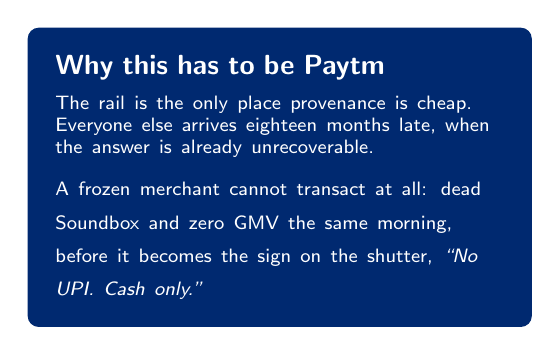
\begin{tikzpicture}\node[rounded corners=4pt,fill=navy,text=white,inner sep=10pt,text width=5.7cm,align=left]{
{\bfseries Why this has to be Paytm}\\[0.45em]
\scriptsize The rail is the only place provenance is cheap. Everyone else arrives eighteen months late, when the answer is already unrecoverable.\\[0.45em]
\scriptsize A frozen merchant cannot transact at all: dead Soundbox and zero GMV the same morning, before it becomes the sign on the shutter, \emph{\qm{No UPI. Cash only.}}
};\end{tikzpicture}
\end{column}
\end{columns}
\vspace{0.4cm}
\begin{center}
{\large\color{navy}\bfseries Paytm Hisaab}\quad{\color{muted}every rupee, on your side.}
\end{center}
\note{{\color{navy}\bfseries\normalsize 15.~The line we do not cross}\par\vspace{0.55em}\textbf{0:30 --- the non-negotiables, fast, then land.}
\\[0.4em]
Run the five bullets at pace. The one to hit is the first: we never assert
innocence on a freeze. The last is the mid-review answer, on the slide on purpose.
\\[0.4em]
Then the navy box: provenance is cheap only on the rail, and a frozen merchant
stops transacting the same morning.
\\[0.4em]
Final line, unhurried: \emph{``Paytm Hisaab. Every rupee, on your side.''} Stop talking.
\\[0.5em]
{\scriptsize
{\color{navy}\bfseries --- Q\&A prep ---}
\\[0.3em]
\textbf{``Merchants may not take personal money on a business QR.''} Correct, and
slide 11 says so before you have to. It arrives anyway, and the alternative to
recording it is letting an authority read it as income. We are not defending the
behaviour --- we are refusing to let it become a liability.
\\[0.3em]
\textbf{``Paytm already tags transactions.''} It does, and we build on that rather
than around it: channel, linked VPAs and payer history feed the rules layer. What
no tag carries is her attestation --- the part an authority accepts, and the only
part she alone can give.
\\[0.3em]
\textbf{``No return mismatch?''} That check needs a \emph{registered} composition
dealer who filed a CMP-08 to disagree with. Ours is unregistered, which is why she
gets a notice at all; the eval split has one with four quarters seeded.
\\[0.3em]
\textbf{``Exempt vs taxable on a QR sale?''} Not per payment. We apportion by value
from that shop's own POS-billed ratio and label it an estimate. Labelling each sale
by its majority side understated taxable turnover threefold.
\\[0.3em]
\textbf{``Four LLM calls in a trenchcoat?''} Everything deterministic is a skill and
four agents is the ceiling. If twenty lines of Python replaces an agent, it should
have been a skill --- the trace shows which is which.
\\[0.3em]
\textbf{``No standing with the police.''} Agreed: Paytm supplies, the merchant
files. By design. Cash sales are real, out of scope, and on the slide.}}
\end{frame}

\end{document}
"
%                                                     -> speaker notes, one page per slide
%
% Speaker notes live in the \note{} after each frame, so they cannot drift
% out of sync with the slides. Build both with: ./build.sh
%
% Fonts: Segoe UI + Nirmala UI (both ship with Windows). On another OS the
% deck still builds -- it falls back to the default sans and drops the
% Kannada styling.
\documentclass[aspectratio=169,10pt]{beamer}

\usepackage{fontspec}
\usepackage{tikz}
\usepackage{booktabs}
\usepackage{array}
\newcolumntype{L}[1]{>{\raggedright\arraybackslash}p{#1}}
\usepackage{graphicx}
\usetikzlibrary{calc,positioning,arrows.meta}

\graphicspath{{./}{../}}

% ---------- fonts ----------
\IfFontExistsTF{Segoe UI}{\setsansfont{Segoe UI}}{}
\IfFontExistsTF{Nirmala UI}{%
  \newfontfamily\kn[Script=Kannada]{Nirmala UI}}{%
  \newcommand{\kn}{}}
\renewcommand{\familydefault}{\sfdefault}

% ragged, unhyphenated text inside the narrow cards
\hyphenpenalty=10000
\exhyphenpenalty=10000
\emergencystretch=3em
\hbadness=10000

% ---------- palette (taken from the product mock) ----------
\definecolor{navy}{HTML}{002970}
\definecolor{ptmcyan}{HTML}{00BAF2}
\definecolor{ink}{HTML}{0F172A}
\definecolor{muted}{HTML}{64748B}
\definecolor{good}{HTML}{15803D}
\definecolor{bad}{HTML}{DC2626}
\definecolor{amber}{HTML}{B45309}
\definecolor{tint}{HTML}{EAF4FD}
\definecolor{hairline}{HTML}{DBE7F3}

% ---------- theme ----------
\usetheme{default}
\usecolortheme{default}
\setbeamertemplate{navigation symbols}{}
\setbeamersize{text margin left=0.85cm,text margin right=0.85cm}
\setbeamercolor{normal text}{fg=ink,bg=white}
\setbeamercolor{frametitle}{fg=navy}
\setbeamercolor{structure}{fg=navy}
\setbeamerfont{frametitle}{size=\large,series=\bfseries}
\setbeamerfont{framesubtitle}{size=\scriptsize}
\setbeamercolor{framesubtitle}{fg=muted}
\setbeamertemplate{frametitle}{%
  \vspace{0.30cm}%
  \usebeamerfont{frametitle}\usebeamercolor[fg]{frametitle}\insertframetitle%
  \ifx\insertframesubtitle\empty\else{\\[-0.15em]\usebeamerfont{framesubtitle}\usebeamercolor[fg]{framesubtitle}\insertframesubtitle}\fi%
  \\[0.1em]{\color{ptmcyan}\rule{1.2cm}{2pt}}\par\vspace{-0.15em}%
}
\setbeamertemplate{footline}{%
  \hbox{\begin{beamercolorbox}[wd=\paperwidth,ht=1.9ex,dp=1.1ex,leftskip=0.85cm,rightskip=0.85cm]{}%
  {\scriptsize\color{muted}Paytm Hisaab\hfill\insertframenumber}%
  \end{beamercolorbox}}%
}
\setbeamerfont{itemize/enumerate body}{size=\normalsize}

% ---------- helpers ----------
\newcommand{\hi}[1]{{\color{navy}\bfseries #1}}
\newcommand{\red}[1]{{\color{bad}\bfseries #1}}
\newcommand{\grn}[1]{{\color{good}\bfseries #1}}
\newcommand{\sub}[1]{{\color{muted}#1}}
\newcommand{\qm}[1]{``#1''}
\newcommand{\bignum}[2]{{\color{navy}\fontsize{22}{24}\selectfont\bfseries #1}\\[0.1em]{\scriptsize\color{muted}#2}}
% a soft rounded card:  \card{width}{body}
\newcommand{\card}[2]{\begin{tikzpicture}%
  \node[rounded corners=4pt,fill=tint,inner sep=8pt,text width=#1,align=left]{#2};%
  \end{tikzpicture}}
% an outlined card:  \ocard{colour}{width}{body}
\newcommand{\ocard}[3]{\begin{tikzpicture}%
  \node[rounded corners=4pt,fill=white,draw=#1,line width=0.9pt,inner sep=8pt,text width=#2,align=left]{#3};%
  \end{tikzpicture}}

% ---------- presenter build ----------
% Set after every colour and template above, so the composed notes page keeps
% the deck's own colours:
%   xelatex -jobname=hisaab-pitch-notes "\def\shownotes{1}% Paytm Hisaab -- buildathon pitch deck
%
% Compile with XeLaTeX (needed for the rupee sign and the Kannada line):
%
%   cd pitch
%   xelatex hisaab-pitch.tex                          -> hisaab-pitch.pdf  (slides)
%   xelatex -jobname=hisaab-pitch-notes "\def\shownotes{1}% Paytm Hisaab -- buildathon pitch deck
%
% Compile with XeLaTeX (needed for the rupee sign and the Kannada line):
%
%   cd pitch
%   xelatex hisaab-pitch.tex                          -> hisaab-pitch.pdf  (slides)
%   xelatex -jobname=hisaab-pitch-notes "\def\shownotes{1}\input{hisaab-pitch.tex}"
%                                                     -> speaker notes, one page per slide
%
% Speaker notes live in the \note{} after each frame, so they cannot drift
% out of sync with the slides. Build both with: ./build.sh
%
% Fonts: Segoe UI + Nirmala UI (both ship with Windows). On another OS the
% deck still builds -- it falls back to the default sans and drops the
% Kannada styling.
\documentclass[aspectratio=169,10pt]{beamer}

\usepackage{fontspec}
\usepackage{tikz}
\usepackage{booktabs}
\usepackage{array}
\newcolumntype{L}[1]{>{\raggedright\arraybackslash}p{#1}}
\usepackage{graphicx}
\usetikzlibrary{calc,positioning,arrows.meta}

\graphicspath{{./}{../}}

% ---------- fonts ----------
\IfFontExistsTF{Segoe UI}{\setsansfont{Segoe UI}}{}
\IfFontExistsTF{Nirmala UI}{%
  \newfontfamily\kn[Script=Kannada]{Nirmala UI}}{%
  \newcommand{\kn}{}}
\renewcommand{\familydefault}{\sfdefault}

% ragged, unhyphenated text inside the narrow cards
\hyphenpenalty=10000
\exhyphenpenalty=10000
\emergencystretch=3em
\hbadness=10000

% ---------- palette (taken from the product mock) ----------
\definecolor{navy}{HTML}{002970}
\definecolor{ptmcyan}{HTML}{00BAF2}
\definecolor{ink}{HTML}{0F172A}
\definecolor{muted}{HTML}{64748B}
\definecolor{good}{HTML}{15803D}
\definecolor{bad}{HTML}{DC2626}
\definecolor{amber}{HTML}{B45309}
\definecolor{tint}{HTML}{EAF4FD}
\definecolor{hairline}{HTML}{DBE7F3}

% ---------- theme ----------
\usetheme{default}
\usecolortheme{default}
\setbeamertemplate{navigation symbols}{}
\setbeamersize{text margin left=0.85cm,text margin right=0.85cm}
\setbeamercolor{normal text}{fg=ink,bg=white}
\setbeamercolor{frametitle}{fg=navy}
\setbeamercolor{structure}{fg=navy}
\setbeamerfont{frametitle}{size=\large,series=\bfseries}
\setbeamerfont{framesubtitle}{size=\scriptsize}
\setbeamercolor{framesubtitle}{fg=muted}
\setbeamertemplate{frametitle}{%
  \vspace{0.30cm}%
  \usebeamerfont{frametitle}\usebeamercolor[fg]{frametitle}\insertframetitle%
  \ifx\insertframesubtitle\empty\else{\\[-0.15em]\usebeamerfont{framesubtitle}\usebeamercolor[fg]{framesubtitle}\insertframesubtitle}\fi%
  \\[0.1em]{\color{ptmcyan}\rule{1.2cm}{2pt}}\par\vspace{-0.15em}%
}
\setbeamertemplate{footline}{%
  \hbox{\begin{beamercolorbox}[wd=\paperwidth,ht=1.9ex,dp=1.1ex,leftskip=0.85cm,rightskip=0.85cm]{}%
  {\scriptsize\color{muted}Paytm Hisaab\hfill\insertframenumber}%
  \end{beamercolorbox}}%
}
\setbeamerfont{itemize/enumerate body}{size=\normalsize}

% ---------- helpers ----------
\newcommand{\hi}[1]{{\color{navy}\bfseries #1}}
\newcommand{\red}[1]{{\color{bad}\bfseries #1}}
\newcommand{\grn}[1]{{\color{good}\bfseries #1}}
\newcommand{\sub}[1]{{\color{muted}#1}}
\newcommand{\qm}[1]{``#1''}
\newcommand{\bignum}[2]{{\color{navy}\fontsize{22}{24}\selectfont\bfseries #1}\\[0.1em]{\scriptsize\color{muted}#2}}
% a soft rounded card:  \card{width}{body}
\newcommand{\card}[2]{\begin{tikzpicture}%
  \node[rounded corners=4pt,fill=tint,inner sep=8pt,text width=#1,align=left]{#2};%
  \end{tikzpicture}}
% an outlined card:  \ocard{colour}{width}{body}
\newcommand{\ocard}[3]{\begin{tikzpicture}%
  \node[rounded corners=4pt,fill=white,draw=#1,line width=0.9pt,inner sep=8pt,text width=#2,align=left]{#3};%
  \end{tikzpicture}}

% ---------- presenter build ----------
% Set after every colour and template above, so the composed notes page keeps
% the deck's own colours:
%   xelatex -jobname=hisaab-pitch-notes "\def\shownotes{1}\input{hisaab-pitch.tex}"
\ifdefined\shownotes
  \setbeamertemplate{note page}{%
    \usebeamercolor[fg]{normal text}%
    \vspace{0.2em}%
    {\scriptsize\color{muted}Paytm Hisaab \;$\cdot$\; speaker notes}\hfill
    {\scriptsize\color{muted}slide \insertframenumber\ of 15}\par
    \vspace{0.25em}{\color{ptmcyan}\rule{\textwidth}{1.5pt}}\par
    \vspace{0.55em}\footnotesize\raggedright\insertnote\par}
  \setbeameroption{show only notes}
\fi

\begin{document}

% ============================================================ 1. TITLE
{\setbeamertemplate{footline}{}
\begin{frame}[plain]
\vspace{0.9cm}
\begin{center}
{\fontsize{38}{42}\selectfont\bfseries\color{navy}Paytm\;\color{ink}Hisaab}\\[0.45em]
{\Large\color{muted}Every rupee, on your side.}\\[0.9em]
{\color{ptmcyan}\rule{2.8cm}{2.5pt}}\\[0.9em]
{\large\color{ink}The agent that lets a merchant account for their own money}\\[0.15em]
{\large\color{ink}when someone in authority demands an explanation.}\\[1.3em]
{\small\color{muted}Agent Labs Buildathon \;$\cdot$\; Phinite $\times$ Paytm \;$\cdot$\; Track 2: AI for Small Businesses}
\end{center}
\note{{\color{navy}\bfseries\normalsize 1.~Title}\par\vspace{0.55em}\textbf{0:10 --- open cold.} Do not read the title or the tagline off the slide.
\\[0.4em]
Say: \emph{``I want to tell you about a man in Haveri who opened an envelope.''} Then advance.
\\[0.4em]
Nothing on this slide needs explaining. The tagline lands at the end, not here.}
\end{frame}}

% ============================================================ 2. STORY
\begin{frame}{Haveri, 2025}{A vegetable vendor opens an envelope}
\vspace{0.05cm}
\begin{columns}[T]
\begin{column}{0.52\textwidth}
\vspace{0.15cm}
He sells vegetables. Vegetables are \hi{exempt} from GST.\\[0.6em]
He also took UPI, because Paytm asked him to.\\[0.6em]
Four years of credits into his account, added up and billed as income:
\begin{center}\vspace{0.1em}{\fontsize{30}{32}\selectfont\bfseries\color{bad}₹29 lakh}\end{center}
\end{column}
\begin{column}{0.44\textwidth}
\ocard{hairline}{5.4cm}{\centering
  {\color{muted}\scriptsize Within weeks, on shutters across Karnataka:}\\[0.6em]
  {\fontsize{20}{23}\selectfont\bfseries\color{ink}\qm{No UPI.\\ Cash only.}}\\[0.6em]
  {\color{muted}\scriptsize A statewide boycott, by the merchants who had just adopted it.}}
\end{column}
\end{columns}
\vspace{0.25cm}
\hspace{0.1cm}{\small\sub{Withdrawn for the traders who could \emph{show} what they sold. Most could not. And tax is no longer the only authority asking.}}
\note{{\color{navy}\bfseries\normalsize 2.~Haveri, 2025}\par\vspace{0.55em}\textbf{0:45 --- the hook. Tell it, do not summarise it.}
\\[0.4em]
Four beats, in this order: he sells vegetables; vegetables are exempt from GST;
he took UPI because \emph{we} asked him to; the department added up four years of
credits and sent him a bill for \textbf{₹29 lakh}.
\\[0.4em]
\textbf{Pause on the number.} Then the card: within weeks, shutters across Karnataka
read ``No UPI, cash only.'' Merchants we had just onboarded, boycotting the rail.
\\[0.4em]
Close on the bottom line --- the notices were withdrawn for traders who could
\emph{show} what they sold. Most could not. That verb is the whole product.
\\[0.4em]
\textbf{Then the bridge:} \emph{``and tax is no longer the only authority asking.''}
That sentence is doing the repositioning --- Haveri is not a tax story here, it is
the moment taking digital money became a liability. The sharper version of it is
two slides away.
\\[0.4em]
\textbf{Do not say this is happening right now.} It is 2025. The next slide is
what makes it current, and a judge who knows the episode will respect the distinction.}
\end{frame}

% ============================================================ 3. STILL HAPPENING
\begin{frame}{And this is not a 2025 story}{CAclubindia, last updated 02 September 2026: ten days ago}
\vspace{0.1cm}
\begin{center}

\includegraphics[width=12.4cm]{gst-notices-2026.png}
\end{center}
\vspace{0.35cm}
\card{13.1cm}{\scriptsize\qm{During August 2026, the GST Department issued a significant number of notices covering different financial years and involving a wide range of issues\ldots\ They covered matters such as ITC mismatches, ineligible credit, \hi{differences in turnover}, wrong GST classification or rate, \hi{exemption claims}, Reverse Charge Mechanism\ldots}}
\vspace{0.3cm}

\hspace{0.1cm}{\small Those two categories are the whole content of an evidence pack. And this is the \emph{slower} of the two authorities. The other one freezes the account first.}
\note{{\color{navy}\bfseries\normalsize 3.~And this is not a 2025 story}\par\vspace{0.55em}\textbf{0:25 --- fast. This slide exists to kill one objection.}
\\[0.4em]
Say: \emph{``That was last year. This was published ten days ago.''}
\\[0.4em]
Do not read the quote. Point at the two bolded phrases only ---
\textbf{differences in turnover} and \textbf{exemption claims} --- and say those
two categories are the entire content of what we build.
\\[0.4em]
\textbf{Land on the last line and move.} It is the handoff into the police
slide: this is the slower authority. The other one freezes first and asks
afterwards. Do not linger here --- tax is no longer the headline.}
\end{frame}

% ============================================================ 4. THE TRAP
\begin{frame}{Every rupee a merchant receives is now evidence}{Today it is only ever used against them}
\vspace{0.05cm}
\begin{columns}[T]
\begin{column}{0.47\textwidth}
\ocard{bad}{6.0cm}{{\bfseries\color{bad}The cyber-crime police}\\[0.35em]
\scriptsize Fraud money layers through accounts within minutes. The shop at the end of the chain, the one that sold someone a watermelon, is frozen. It did nothing wrong, is not named in the FIR, and finds out when a payment declines.}
\end{column}
\begin{column}{0.47\textwidth}
\card{6.1cm}{{\bfseries\color{navy}The tax department}\\[0.35em]
\scriptsize Compares UPI collections against filed returns and bills the difference. Registered traders too, with QR, wallet, card and cash deposits all in scope.}
\end{column}
\end{columns}
\vspace{0.4cm}
\begin{center}
{\large Both demand the same artefact: \hi{what was each rupee, actually?}}\\[0.3em]
{\small\color{muted}Paytm already sees more of this than anyone. What is missing is the \emph{merchant's own answer}, captured when it is still knowable.}
\end{center}
\vspace{0.15cm}
{\color{hairline}\hrule height 1pt}
\vspace{0.35em}
\hspace{0.05cm}{\scriptsize\bfseries\color{bad}What it costs Paytm:}~{\scriptsize a frozen merchant stops transacting that morning. A frightened one takes the QR down for good. Dead Soundbox, zero GMV, no lending origination.}
\note{{\color{navy}\bfseries\normalsize 4.~Every rupee is now evidence}\par\vspace{0.55em}\textbf{0:40 --- two authorities, one unanswerable question.}
\\[0.4em]
\textbf{Left card first and give it the time.} Fraud money layers within minutes,
and the shop at the end of the chain, \emph{the one that sold someone a watermelon},
gets frozen. It did nothing wrong, it is not named in the FIR, and it finds out
when a payment declines. Use the watermelon.
\\[0.4em]
Right card briskly: the department reconciles collections against filed returns
and bills the difference. One sentence, then move.
\\[0.4em]
Then the pivot: both demand the same artefact --- what was each rupee, actually.
\\[0.4em]
\textbf{Say the grey line as written.} We do \emph{not} claim Paytm does nothing
with this data --- it tags plenty. The gap is the merchant's own answer, captured
when it is still knowable. Claiming otherwise in this room gets corrected.
\\[0.4em]
\textbf{Slow down for the red line.} This is the business case, not a footnote:
a frozen merchant stops transacting that morning, a frightened one takes the QR
down for good. Dead Soundbox, zero GMV, no lending origination.}
\end{frame}

% ============================================================ 5. THE BAR
\begin{frame}{Gross credits are not turnover}{One shop, one year, ₹60.98 lakh of credits}
\vspace{0.1cm}
\begin{center}
\begin{tikzpicture}[x=1cm,y=1cm]
% --- what the notice counts
\node[anchor=west,font=\scriptsize\bfseries,text=bad] at (-0.05,1.80) {WHAT THE NOTICE COUNTS AS TURNOVER};
\fill[bad!85,rounded corners=2pt] (0,1.06) rectangle (11.4,1.60);
\node[font=\small\bfseries,text=white] at (5.7,1.33) {₹60.98 lakh};

% --- what actually happened   (1 lakh = 0.18696 cm, so the bars are the same length)
\node[anchor=west,font=\scriptsize\bfseries,text=navy] at (-0.05,0.66) {WHAT ACTUALLY HAPPENED};
\fill[good!80,rounded corners=2pt]  (0,-0.08)     rectangle (6.001,0.46);
\fill[good!45]                      (6.001,-0.08) rectangle (8.002,0.46);
\fill[ptmcyan!70]                   (8.002,-0.08) rectangle (9.385,0.46);
\fill[navy!55]                      (9.385,-0.08) rectangle (10.451,0.46);
\fill[amber!70]                     (10.451,-0.08)rectangle (11.255,0.46);
\fill[muted!60,rounded corners=2pt] (11.255,-0.08)rectangle (11.4,0.46);

% brackets
\draw[navy,line width=0.8pt] (0,-0.22) -- (0,-0.36) -- (8.002,-0.36) -- (8.002,-0.22);
\node[anchor=north,font=\scriptsize,text=navy,align=center] at (4.0,-0.38)
  {\bfseries ₹42.9L aggregate turnover\quad{\color{muted}\scriptsize exempt ₹32.1L + taxable ₹10.7L}};
\draw[bad,line width=0.8pt] (8.002,-0.22) -- (8.002,-0.36) -- (11.4,-0.36) -- (11.4,-0.22);
\node[anchor=north,font=\scriptsize,text=bad,align=center] at (9.7,-0.38)
  {\bfseries ₹18.1L that is not turnover at all};

% legend
\node[font=\scriptsize,text=ink] at (5.7,-1.02) {%
\textcolor{good!80}{$\blacksquare$}~Exempt sales \quad
\textcolor{good!45}{$\blacksquare$}~Taxable sales \quad
\textcolor{ptmcyan!70}{$\blacksquare$}~Her own accounts ₹7.4L};
\node[font=\scriptsize,text=ink] at (5.7,-1.40) {%
\textcolor{navy!55}{$\blacksquare$}~Family ₹5.7L \quad
\textcolor{amber!70}{$\blacksquare$}~Loans, chit, gifts ₹4.3L \quad
\textcolor{muted!60}{$\blacksquare$}~Refunds \& duplicates ₹0.7L};
\end{tikzpicture}
\end{center}
\vspace{0.15cm}
\hspace{0.1cm}{\small\sub{Personal money does not belong on a business QR. It arrives anyway, reads as turnover, and hides the one credit the police will ask about.}}
\note{{\color{navy}\bfseries\normalsize 5.~Gross credits are not turnover}\par\vspace{0.55em}\textbf{0:45 --- the hinge of the pitch. Let the picture work.}
\\[0.4em]
Say: \emph{``One shop, one year, ₹60.98 lakh of credits. The red bar is what the
notice counts as turnover --- all of it.''}
\\[0.4em]
Then the bottom bar. \textbf{Stop talking for two seconds} and let them read it.
\\[0.4em]
₹42.9L really is turnover, and we say so. ₹18.1L is not: her savings account, her
husband, a chit payout, a double-tap on the Soundbox.
\\[0.4em]
\textbf{Get in front of the obvious objection.} Personal money is not supposed to
touch a business QR. Say so first, then say it arrives anyway --- that is an
observation about merchants, not a loophole we are selling. The rule does not stop
it; it only means no one is keeping a record of it.
\\[0.4em]
\textbf{And close on the second use.} This volume is also why she cannot find the
one credit the police care about. Same bar, same problem, and the freeze slide
pays it off.
\\[0.4em]
If challenged on the numbers: seeded ground truth from our generator, not an
estimate. Accuracy against it is slide 14.}
\end{frame}

% ============================================================ 6. INSIGHT
\begin{frame}{The insight}{Most teams would build the tax tool \emph{or} the fraud tool. They are the same engine.}
\vspace{0.15cm}
\begin{center}
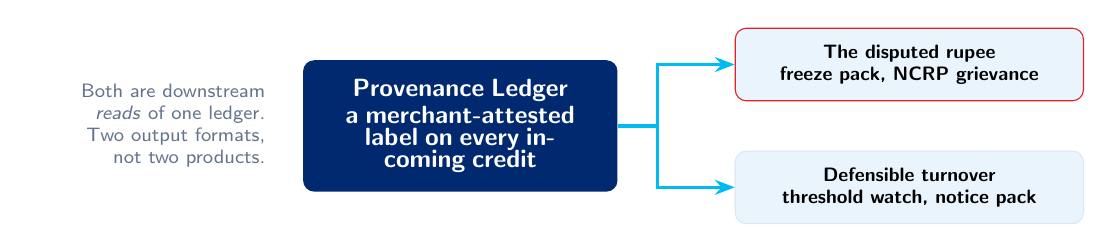
\begin{tikzpicture}[font=\scriptsize]
\node[rounded corners=4pt,fill=navy,text=white,inner sep=7pt,align=center,text width=3.5cm]
  (eng) {\bfseries\small Provenance Ledger\\[0.15em] a merchant-attested label on every incoming credit};
\node[rounded corners=4pt,fill=tint,draw=bad,inner sep=6pt,align=center,text width=4.0cm]
  (tax) at ($(eng.east)+(3.7,0.78)$) {\bfseries The disputed rupee\\ freeze pack, NCRP grievance};
\node[rounded corners=4pt,fill=tint,draw=hairline,inner sep=6pt,align=center,text width=4.0cm]
  (fra) at ($(eng.east)+(3.7,-0.78)$) {\bfseries Defensible turnover\\ threshold watch, notice pack};
\draw[-{Stealth[length=2.5mm]},ptmcyan,line width=1.3pt] (eng.east) -- ++(0.5,0) |- (tax.west);
\draw[-{Stealth[length=2.5mm]},ptmcyan,line width=1.3pt] (eng.east) -- ++(0.5,0) |- (fra.west);
\node[anchor=east,text width=2.9cm,align=right,text=muted] at ($(eng.west)+(-0.35,0)$)
  {Both are downstream \emph{reads} of one ledger. Two output formats, not two products.};
\end{tikzpicture}
\end{center}
\vspace{0.1cm}
\begin{center}
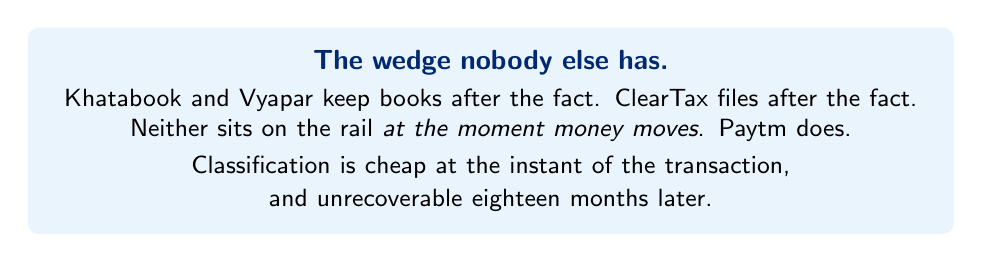
\begin{tikzpicture}\node[rounded corners=4pt,fill=tint,inner sep=8pt,text width=11.2cm,align=center]{
{\bfseries\color{navy}The wedge nobody else has.}\\[0.25em]
\small Khatabook and Vyapar keep books after the fact. ClearTax files after the fact.\\
Neither sits on the rail \emph{at the moment money moves}. Paytm does.\\[0.25em]
\small Classification is cheap at the instant of the transaction,\\ and unrecoverable eighteen months later.
};\end{tikzpicture}
\end{center}
\note{{\color{navy}\bfseries\normalsize 6.~The insight}\par\vspace{0.55em}\textbf{0:40 --- why this is one product, not two.}
\\[0.4em]
Say: \emph{``Most teams would build the fraud tool or the tax tool. They are the
same engine.''} Both are downstream reads of one ledger --- two output formats,
and the freeze pack is the one we lead with.
\\[0.4em]
Then the wedge, and say it slowly because it is the defensible-moat answer:
Khatabook and Vyapar keep books after the fact, ClearTax files after the fact.
Neither sits on the rail at the moment money moves. \textbf{Paytm does.}
\\[0.4em]
Landing line: classification is cheap and accurate at the instant of the
transaction, and unrecoverable eighteen months later when the notice arrives.}
\end{frame}

% ============================================================ 7. THE ENGINE
\begin{frame}{The engine}{Eight tags, one tap}
\vspace{0.15cm}
\begin{columns}[T]
\begin{column}{0.45\textwidth}
{\color{navy}\bfseries\small Every incoming credit gets one tag}\\[0.4em]
{\scriptsize
\begin{tabular}{@{}ll@{}}
\texttt{taxable\_supply}    & ordinary sale \\
\texttt{exempt\_supply}     & vegetables, milk, loose rice \\
\texttt{personal\_transfer} & spouse, parent, sibling \\
\texttt{inter\_account}     & her own money \\
\texttt{refund\_reversal}   & money back from a vendor \\
\texttt{duplicate}          & paid twice, one refunded \\
\texttt{non\_business}      & loan, chit payout, gift \\
{\color{bad}\texttt{unclassified}} & {\color{bad}not enough signal: ask her} \\
\end{tabular}}
\\[0.75em]
{\scriptsize\color{muted}98.6\% are ordinary sales, settled by rules. The agent reasons only about the 1.4\% that need judgement.}
\end{column}
\begin{column}{0.51\textwidth}
\card{6.6cm}{{\bfseries\color{navy}The agent proposes. The merchant attests.}\\[0.4em]
\scriptsize You cannot infer \qm{my husband sent this} from a QR payment. The agent proposes a tag \emph{with its reason}; she confirms with one tap, in Kannada, batched daily.\\[0.45em]
\scriptsize Not a fallback. A ledger she attested \emph{at the time} survives a hearing. An algorithm's guess, made under duress a year later, does not.}
\\[0.55em]
\hspace{0.15cm}\begin{minipage}{6.6cm}
{\bfseries\color{navy}\small Budget: at most 3 questions a day.}\\[0.15em]
{\scriptsize\color{muted}Over a simulated year: \hi{189 questions, median 1.3 a day}. Ask more and the product is dead.}
\end{minipage}
\end{column}
\end{columns}
\note{{\color{navy}\bfseries\normalsize 7.~The engine}\par\vspace{0.55em}\textbf{0:45 --- the mechanism. Do not read the tag list.}
\\[0.4em]
Gesture at the eight tags, say ``eight labels, every incoming credit gets one,''
and move to the right-hand card, which is the real content.
\\[0.4em]
\textbf{The line that matters:} you cannot infer ``my husband sent this'' from a
QR payment. So the agent proposes a tag \emph{with its reason} and she confirms
with one tap. This is not a fallback --- a ledger she attested contemporaneously
survives a hearing; an algorithm's guess produced under duress a year later does not.
\\[0.4em]
Then the budget: at most three questions a day, and we measured 189 across a
year, median 1.3. Ask more than that and the product is dead.
\\[0.4em]
If asked about cost: 98.6\% are ordinary sales settled by rules. The model only
sees the 1.4\% that need judgement.}
\end{frame}

% ============================================================ 8. PRODUCT
\begin{frame}{What the merchant sees}
\vspace{-0.1cm}
\begin{center}
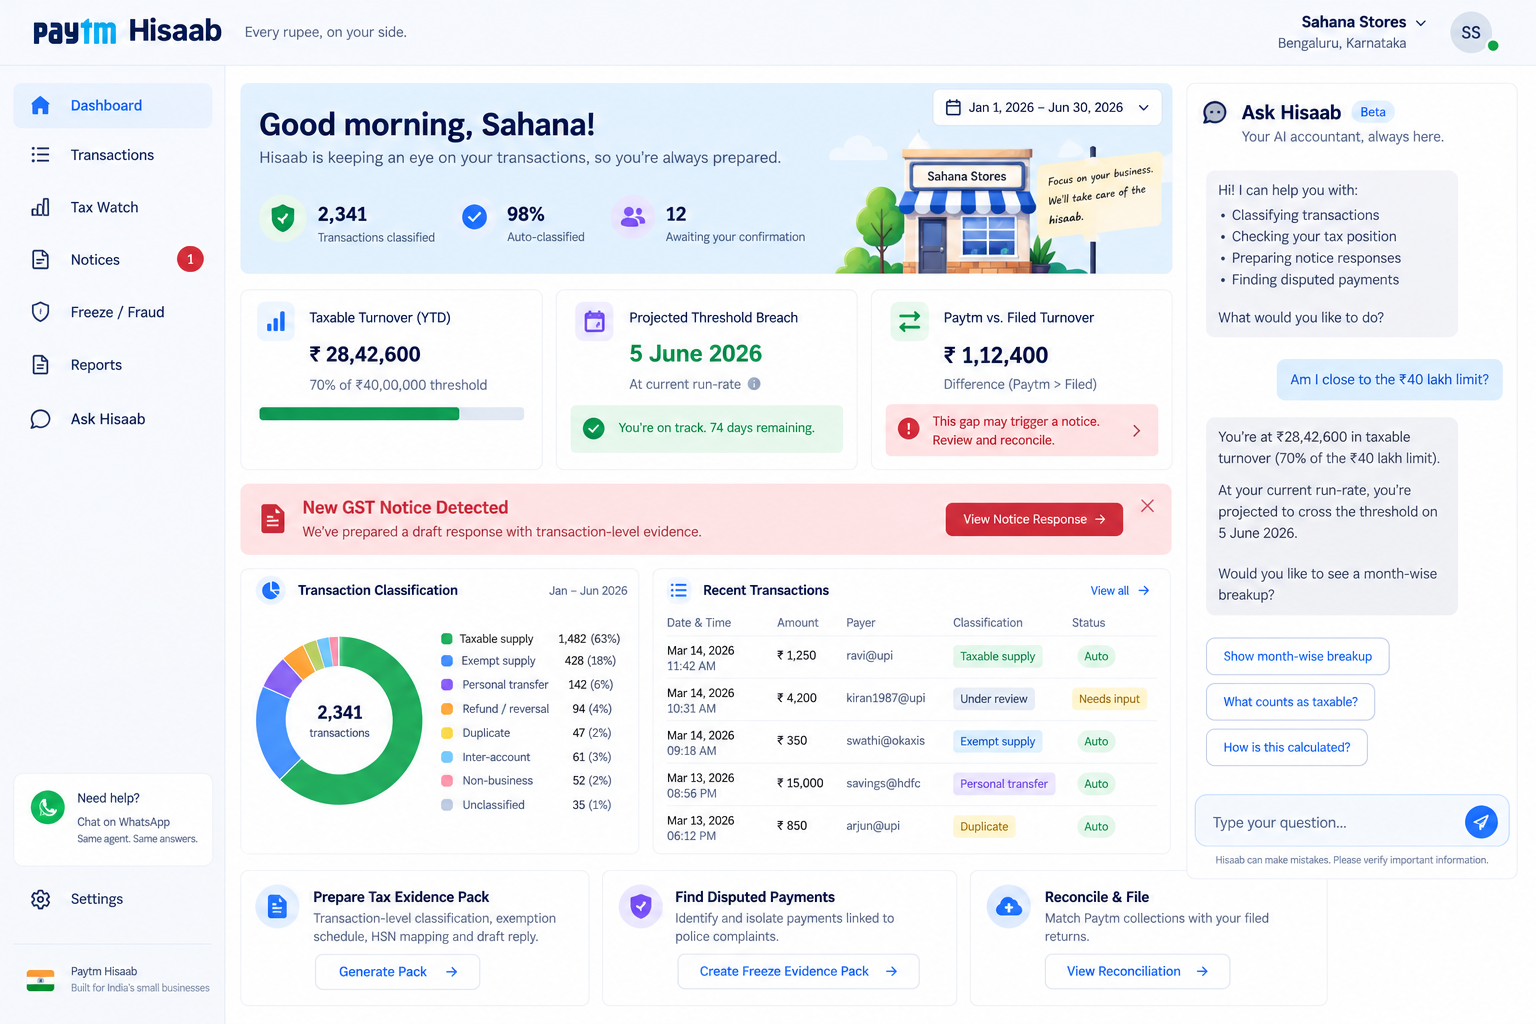
\includegraphics[width=\textwidth,height=0.70\textheight,keepaspectratio]{Paytm-Hisaab_website_look.png}
\end{center}
\vspace{0.1cm}
\hspace{0.05cm}{\scriptsize\color{muted}One surface: what every payment was classified as, how close she is to the threshold, and the packs. The same agent runs on WhatsApp, where she actually is.}
\note{{\color{navy}\bfseries\normalsize 8.~What the merchant sees}\par\vspace{0.55em}\textbf{0:20 --- a glance slide. Do not tour the UI.}
\\[0.4em]
One sentence: everything classified, how close she is to the threshold, and the
packs, on one surface.
\\[0.4em]
Then the WhatsApp point --- the same agent, where she actually is --- and advance.
\\[0.4em]
If someone asks whether this is built: the chat and the tools are live; this
screen is the product surface we are designing toward.}
\end{frame}

% ============================================================ 9. ARCHITECTURE
\begin{frame}{Built on Phinite}{Two agent graphs, four agents, ten deterministic skills}
\vspace{0.15cm}
\begin{columns}[T]
\begin{column}{0.53\textwidth}
{\scriptsize
\begin{tabular}{@{}L{1.75cm}L{4.7cm}@{}}
\multicolumn{2}{@{}l}{\color{navy}\bfseries\small hisaab-watch \;\scriptsize(autonomous: cron + API)}\\
\midrule
Provenance & proposes a tag and a reason for the hard credits \\
Evidence   & assembles packs: freeze evidence, then exemption schedules and HSN \\
\addlinespace[0.6em]
\multicolumn{2}{@{}l}{\color{navy}\bfseries\small hisaab-merchant \;\scriptsize(conversational: chat)}\\
\midrule
Merchant   & the conversation: attestation, alerts, Kannada \\
Escalation & decides when to stop and route to a human CA \\
\bottomrule
\end{tabular}}
\\[0.75em]
{\scriptsize\color{muted}The nightly pass writes its queue to the ledger; the chat reads it when she opens it. Deliberately \emph{not} a graph-to-graph call: a queue that outlives either run is what makes the handoff robust.}
\end{column}
\begin{column}{0.44\textwidth}
\card{5.7cm}{{\bfseries\color{navy}Permissions are the product}\\[0.4em]
\scriptsize Provenance proposes, \red{never commits}.\\[0.25em]
\scriptsize Merchant is the \emph{only} agent that can commit a tag.\\[0.25em]
\scriptsize Evidence is \red{read-only}. It cannot edit a classification to make a pack look better.\\[0.25em]
\scriptsize Escalation can \red{halt} any pack; a human approves.}
\\[0.5em]
\hspace{0.1cm}\begin{minipage}{5.7cm}{\scriptsize\color{muted}Ten tools run live against a hosted service. Every number in a pack traces back, in the trace, to the credit and the attestation behind it.}\end{minipage}
\end{column}
\end{columns}
\note{{\color{navy}\bfseries\normalsize 9.~Built on Phinite}\par\vspace{0.55em}\textbf{0:40 --- for the technical judges.}
\\[0.4em]
Two agent graphs, not four loose agents: \texttt{hisaab-watch} runs autonomously on
cron, \texttt{hisaab-merchant} is the conversation. The nightly pass writes a queue;
the chat reads it when she opens it --- deliberately not a graph-to-graph call,
because a queue that outlives either run is what makes the handoff robust.
\\[0.4em]
\textbf{Spend your time on the right-hand card.} The strongest line in it:
the Evidence agent is read-only --- \emph{the agent that builds the defence cannot
edit the evidence.} And only the Merchant agent can commit an attested tag.
\\[0.4em]
Those are enforced as Phinite tool policies, not conventions, and a denied call
shows up in the trace.}
\end{frame}

% ============================================================ 10. DESIGN DECISIONS
\begin{frame}{Four decisions that make it defensible}
\vspace{0.3cm}
\begin{columns}[T]
\begin{column}{0.48\textwidth}
\card{6.0cm}{{\bfseries\color{navy}1. Arithmetic lives in skills, not the model}\\[0.35em]
\scriptsize Turnover, projections and apportionment are deterministic Python: versioned, testable, traceable. Wrapping arithmetic in an LLM is the standard tell, and the trace would show it.}
\\[0.35em]
\card{6.0cm}{{\bfseries\color{navy}3. Refusing to guess is a feature}\\[0.35em]
\scriptsize An \texttt{unclassified} credit routed to the merchant costs one tap. A confident wrong tag inside an evidence pack is a catastrophe. We report the refusal rate honestly.}
\end{column}
\begin{column}{0.48\textwidth}
\card{6.0cm}{{\bfseries\color{navy}2. Attestation is the promotion boundary}\\[0.35em]
\scriptsize Nothing enters a production pack that the merchant has not confirmed. Sandbox to UAT to prod, with her tap as the gate.}
\\[0.35em]
\card{6.0cm}{{\bfseries\color{navy}4. Ground truth, so accuracy is a number}\\[0.35em]
\scriptsize We simulated a year of a shop's life from a known process, split into what Paytm can see and what really happened. Agents read only the visible half, which is why we quote error bars instead of vibes.}
\end{column}
\end{columns}
\note{{\color{navy}\bfseries\normalsize 10.~Four decisions}\par\vspace{0.55em}\textbf{0:35 --- the slide that separates you from a demo.}
\\[0.4em]
Lead with \#1: all arithmetic is deterministic Python, not model output. Wrapping
arithmetic in an LLM is the standard tell, and the trace would show it.
\\[0.4em]
Then \#3: refusing to guess is a feature. An \texttt{unclassified} credit costs one
tap; a confident wrong tag inside an evidence pack is a catastrophe.
\\[0.4em]
Skim \#2 and \#4 --- one clause each. \#4 is worth a beat if the room is technical:
we generated ground truth, so accuracy is a number instead of a claim.}
\end{frame}

% ============================================================ 11. DEMO / ATTESTATION
\begin{frame}{Demo $\cdot$ Sahana Stores, Jayanagar}{An ordinary Tuesday, before anything goes wrong}
\vspace{0.1cm}
\begin{columns}[T]
\begin{column}{0.48\textwidth}
{\scriptsize\color{muted}Tuesday 10 March. Thirty-nine credits came in over the weekend. The agent asks about \hi{three}.}
\\[0.4em]
\card{5.9cm}{{\kn\scriptsize ಭಾನುವಾರ ರಾತ್ರಿ ₹15,000. ನಿಮ್ಮ ಸ್ವಂತ ಹಣವೇ?}\\[0.25em]
{\color{muted}\scriptsize \qm{₹15,000 at 11:04pm Sunday, from your savings account. Your own money?}}\\[0.35em]
{\scriptsize\color{navy}\fbox{\kn ಹೌದು}\;\fbox{\kn ಇಲ್ಲ}}}
\\[0.4em]
{\scriptsize $\cdot$\; ₹7,500 from her husband, scanned at the shop QR\\[0.25em]
$\cdot$\; ₹4,850 from Raghu Shetty, who has bought twice before. A real sale, and the agent \emph{asks} rather than assumes.}
\\[0.4em]
{\scriptsize\color{muted}The other thirty-six settle silently, and a ₹23 payment nobody can place is left alone.}
\end{column}
\begin{column}{0.48\textwidth}
\ocard{amber}{6.1cm}{{\bfseries\color{amber}And yes, two of those three should not be there}\\[0.35em]
\scriptsize A business QR is not for personal money, and the terms say so. It arrives anyway: family, own top-ups, a chit payout. The rule does not prevent it. It only means \emph{nobody keeps a record of it.}}
\\[0.45em]
{\scriptsize Paytm already reads the signals: channel, linked VPAs, payer history. What no system has is the \hi{merchant's own answer}, given at the time, in her language, and kept.}
\\[0.45em]
{\scriptsize That record is what the next two slides are built from: first for the police, then for the department.}
\end{column}
\end{columns}
\note{{\color{navy}\bfseries\normalsize 11.~Demo --- an ordinary Tuesday (beat 1)}\par\vspace{0.55em}\textbf{0:45 --- or hand over to the live demo here.}
\\[0.4em]
Thirty-nine credits came in over the weekend, the agent asks about \textbf{three}.
Read the Kannada line if you can; otherwise read the gloss under it.
\\[0.4em]
\textbf{Do not hide from the right-hand card --- lead with it.} The mid-review
point was that personal money is not allowed on a business QR. Correct, and we say
so on the slide. The argument is that the rule does not stop it, it only means no
one records it, and an unrecorded credit is what an authority later reads as income.
\\[0.4em]
\textbf{Second half of that card matters just as much.} We are not claiming Paytm
does nothing. It already reads channel, linked VPAs and payer history. What no
system has is her own answer, captured while it is still knowable. That is the
product, and it is a smaller, truer claim than the one we started with.
\\[0.4em]
\textbf{Before going on stage:} confirm the attestation queue is whole ---
\texttt{pending\_total} must be 3. A rehearsal that taps through this beat spends the
queue, and Render needs a clear-cache redeploy to restore it.}
\end{frame}

% ============================================================ 12. DEMO / THE FREEZE
\begin{frame}{Demo $\cdot$ The emergency}{The account is frozen at 09:30 and the supplier payment is due}
\vspace{0.2cm}
\begin{columns}[T]
\begin{column}{0.46\textwidth}
{\scriptsize She sold someone 12kg of onions. That customer was three layers downstream of a fraud victim. She is not named in the FIR, which was filed in another state, and \hi{339 payments} came in that week.}
\\[0.5em]
\card{5.8cm}{{\bfseries\color{navy}The agent isolates it}\\[0.35em]
\scriptsize ₹4,200 on 21 March at 19:47, till POS01. Matched by UTR \emph{and independently} by amount and date.\\[0.3em]
\scriptsize The sale record comes with it: the POS bill, the items, the till and the minute.}
\end{column}
\begin{column}{0.49\textwidth}
\ocard{amber}{6.1cm}{{\bfseries\color{amber}And the decoy it did not choose}\\[0.35em]
\scriptsize A \emph{second} ₹4,200 that same week, from a regular customer. Listed in the pack, and explicitly \emph{not} named as the disputed one. Only the date separates them.}
\\[0.5em]
{\scriptsize Then it drafts the NCRP-CFCFRMS grievance, citing the judgments that only the \emph{disputed amount} should be lien-marked, not the whole account.}
\\[0.5em]
{\scriptsize\color{bad}\bfseries It never asserts that she is innocent.}\\[0.1em]
{\scriptsize\color{muted}Some frozen accounts genuinely are mule accounts. The agent assembles evidence; a human decides. Escalation holds the pack for approval.}
\end{column}
\end{columns}
\note{{\color{navy}\bfseries\normalsize 12.~Demo --- the emergency (beat 4)}\par\vspace{0.55em}\textbf{0:50 --- this is now the lead case. Give it the most time of the three.}
\\[0.4em]
Set the stakes in one sentence: account frozen at half nine, supplier payment due,
339 payments came in that week, and she is not named in the FIR.
\\[0.4em]
\textbf{Why this one leads.} She did nothing wrong and there is no rule she broke.
She sold onions to a customer who turned out to be laundering. Every objection
available against the tax case --- she should not have taken personal money on that
QR, she should have registered --- has no purchase here at all.
\\[0.4em]
The agent isolates ₹4,200 by UTR \emph{and independently} by amount and date, and
brings the POS bill with it --- the items, till POS01, 19:47.
\\[0.4em]
\textbf{The decoy is the point.} A second ₹4,200 that same week from a regular
customer, listed in the pack and explicitly not chosen. Anyone can match an amount;
the pack shows its work.
\\[0.4em]
Finish on the red line: it never asserts she is innocent. Some frozen accounts
genuinely are mule accounts. We assemble evidence; a human decides, and Escalation
holds the pack for approval.}
\end{frame}

% ============================================================ 13. DEMO / TAX
\begin{frame}{Demo $\cdot$ The warning, and the notice}{The same ledger, read for the other authority}
\vspace{0.15cm}
\begin{columns}[T]
\begin{column}{0.38\textwidth}
{\scriptsize\color{muted}Replayed as of 31 January:}
\\[0.35em]
\ocard{good}{4.8cm}{{\bfseries\color{ink}\scriptsize\qm{At your current rate you cross ₹40 lakh around {\color{bad}14 March}. You will need to register.}}\\[0.35em]
{\scriptsize\color{muted}\grn{43 days of warning}, and the date is computed, not typed.}}
\\[0.45em]
{\scriptsize\color{bad}\bfseries This beat is what makes the pitch safe.}\\[0.1em]
{\scriptsize\color{muted}Its first act on the tax side is telling her to register.}
\end{column}
\begin{column}{0.58\textwidth}
{\scriptsize\color{muted}Then the notice arrives, claiming {\color{bad}\bfseries ₹60.98L} of turnover:}
\\[0.3em]
{\scriptsize
\begin{tabular}{@{}lr@{\hskip 1.2em}l@{}}
\multicolumn{2}{@{}l}{\color{navy}\bfseries Aggregate turnover \quad ₹42.2L} & \sub{within \grn{1.6\%} of truth} \\
\midrule
Exempt supplies      & ₹31.3L & \sub{vegetables, loose rice} \\
Taxable supplies     & ₹10.9L & \sub{branded goods, oil, soap} \\
\addlinespace[0.45em]
\multicolumn{2}{@{}l}{\color{navy}\bfseries Not turnover at all \quad ₹18.8L} & \sub{every line traced} \\
\midrule
Her own accounts     & ₹7.4L & \sub{top-ups before supplier runs} \\
Family               & ₹6.1L & \sub{spouse, parent, in-law} \\
Loans, chit, gifts   & ₹4.3L & \sub{chit payout, festival gifts} \\
Refunds, duplicates  & ₹1.0L & \sub{crate returns, double-taps} \\
\bottomrule
\end{tabular}}
\\[0.45em]
{\scriptsize And it says plainly: \hi{the claim is wrong, and you \emph{did} cross ₹40 lakh on 14 March. You must register.}}
\end{column}
\end{columns}
\note{{\color{navy}\bfseries\normalsize 13.~Demo --- the warning and the notice (beats 2 and 3)}\par\vspace{0.55em}\textbf{0:50 --- two tax beats on one slide, deliberately compressed.}
\\[0.4em]
Left: replayed as of 31 January, the agent says she crosses ₹40 lakh around
14 March. \textbf{Say the red line out loud} --- its first act on the tax side is
telling her she owes a registration. That is what stops the room turning hostile.
\\[0.4em]
Right: the notice claims ₹60.98 lakh, and the pack answers it line by line, every
figure traceable to transaction IDs. Then the honest half:
\textbf{the claim is wrong, and she did cross ₹40 lakh, and she must register.}
\\[0.4em]
\textbf{If a judge diffs this against slide 5:} slide 5 shows seeded truth
(₹42.9L), this shows what our system computed (₹42.2L). The 1.6\% between them
\emph{is} the accuracy claim --- say that, do not hedge.
\\[0.4em]
\textbf{If pushed on the personal and own-account lines:} same answer as slide 11.
Those credits should not be on a business QR, they are there anyway, and the
alternative to classifying them is letting them be read as income.}
\end{frame}

% ============================================================ 14. NUMBERS
\begin{frame}{What we can actually prove}{One merchant, one year, 13,267 credits, scored against seeded truth}
\vspace{0.45cm}
\begin{columns}[T]
\begin{column}{0.33\textwidth}
\begin{center}\bignum{1.6\%}{error on aggregate turnover\\ (taxable share within 1\%)}\end{center}
\vspace{0.55cm}
\begin{center}\bignum{43 days}{of warning before the\\ threshold crossing}\end{center}
\end{column}
\begin{column}{0.33\textwidth}
\begin{center}\bignum{1.3 a day}{median questions asked.\\ 189 in a year, never over 3}\end{center}
\vspace{0.55cm}
\begin{center}\bignum{zero}{credits left untagged\\ across the whole year}\end{center}
\end{column}
\begin{column}{0.30\textwidth}
\card{3.8cm}{{\bfseries\color{navy}The honest baseline}\\[0.35em]
\scriptsize A 50-line rules-only classifier gets 99.3\% on sale vs not-a-sale, but catches only \red{77.8\%} of non-sale credits.\\[0.3em]
\scriptsize That residue alone puts two eval merchants on the \emph{wrong side} of ₹40L.\\[0.3em]
\scriptsize Closing it is what the agent plus one tap is for.}
\end{column}
\end{columns}
\vspace{0.45cm}
\hspace{0.1cm}{\scriptsize\color{muted}She corrected the agent 52 times that year. Those corrections are the ledger's strongest evidence, not its failures.}
\note{{\color{navy}\bfseries\normalsize 14.~What we can actually prove}\par\vspace{0.55em}\textbf{0:30 --- do not read all four. Pick two.}
\\[0.4em]
Lead with \textbf{1.6\%} error on turnover and \textbf{1.3 questions a day}. The
other two are there to be read, not narrated.
\\[0.4em]
\textbf{The credibility move is the box on the right} --- volunteer the weakness
before anyone finds it. A rules-only baseline gets 99.3\% on sale vs not-a-sale
but catches only 77.8\% of non-sale credits, and that residue alone puts two eval
merchants on the wrong side of ₹40 lakh. Closing it is what the agent plus one tap is for.
\\[0.4em]
Last line if you have the beat: she corrected the agent 52 times that year, and
those corrections are the ledger's strongest evidence, not its failures.}
\end{frame}

% ============================================================ 15. CLOSE
\begin{frame}{The line we do not cross}{Accuracy, not minimisation}
\vspace{0.3cm}
\begin{columns}[T]
\begin{column}{0.52\textwidth}
{\scriptsize
$\cdot$\; We \hi{never assert innocence} on a freeze. Some accounts really are mule accounts. We assemble evidence; a human decides.\\[0.5em]
$\cdot$\; We \hi{file nothing} with any authority. Artefacts only; the merchant or their CA files.\\[0.5em]
$\cdot$\; We compute what she \hi{genuinely owes} and say so plainly, including \qm{you crossed the threshold, you must register.}\\[0.5em]
$\cdot$\; We \hi{never assert a final liability}. We compute, show the workings, and route to a CA.\\[0.5em]
$\cdot$\; A business QR is \hi{not for personal money}. We do not excuse it. We record it, so it is not read as income.}
\end{column}
\begin{column}{0.44\textwidth}
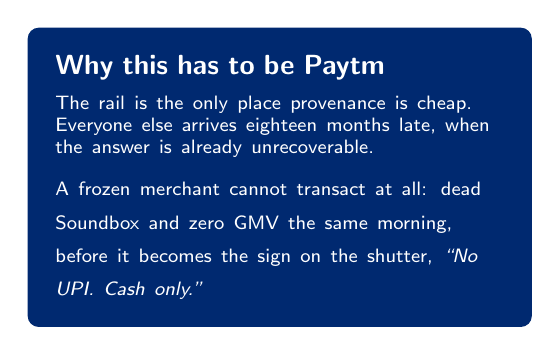
\begin{tikzpicture}\node[rounded corners=4pt,fill=navy,text=white,inner sep=10pt,text width=5.7cm,align=left]{
{\bfseries Why this has to be Paytm}\\[0.45em]
\scriptsize The rail is the only place provenance is cheap. Everyone else arrives eighteen months late, when the answer is already unrecoverable.\\[0.45em]
\scriptsize A frozen merchant cannot transact at all: dead Soundbox and zero GMV the same morning, before it becomes the sign on the shutter, \emph{\qm{No UPI. Cash only.}}
};\end{tikzpicture}
\end{column}
\end{columns}
\vspace{0.4cm}
\begin{center}
{\large\color{navy}\bfseries Paytm Hisaab}\quad{\color{muted}every rupee, on your side.}
\end{center}
\note{{\color{navy}\bfseries\normalsize 15.~The line we do not cross}\par\vspace{0.55em}\textbf{0:30 --- the non-negotiables, fast, then land.}
\\[0.4em]
Run the five bullets at pace. The one to hit is the first: we never assert
innocence on a freeze. The last is the mid-review answer, on the slide on purpose.
\\[0.4em]
Then the navy box: provenance is cheap only on the rail, and a frozen merchant
stops transacting the same morning.
\\[0.4em]
Final line, unhurried: \emph{``Paytm Hisaab. Every rupee, on your side.''} Stop talking.
\\[0.5em]
{\scriptsize
{\color{navy}\bfseries --- Q\&A prep ---}
\\[0.3em]
\textbf{``Merchants may not take personal money on a business QR.''} Correct, and
slide 11 says so before you have to. It arrives anyway, and the alternative to
recording it is letting an authority read it as income. We are not defending the
behaviour --- we are refusing to let it become a liability.
\\[0.3em]
\textbf{``Paytm already tags transactions.''} It does, and we build on that rather
than around it: channel, linked VPAs and payer history feed the rules layer. What
no tag carries is her attestation --- the part an authority accepts, and the only
part she alone can give.
\\[0.3em]
\textbf{``No return mismatch?''} That check needs a \emph{registered} composition
dealer who filed a CMP-08 to disagree with. Ours is unregistered, which is why she
gets a notice at all; the eval split has one with four quarters seeded.
\\[0.3em]
\textbf{``Exempt vs taxable on a QR sale?''} Not per payment. We apportion by value
from that shop's own POS-billed ratio and label it an estimate. Labelling each sale
by its majority side understated taxable turnover threefold.
\\[0.3em]
\textbf{``Four LLM calls in a trenchcoat?''} Everything deterministic is a skill and
four agents is the ceiling. If twenty lines of Python replaces an agent, it should
have been a skill --- the trace shows which is which.
\\[0.3em]
\textbf{``No standing with the police.''} Agreed: Paytm supplies, the merchant
files. By design. Cash sales are real, out of scope, and on the slide.}}
\end{frame}

\end{document}
"
%                                                     -> speaker notes, one page per slide
%
% Speaker notes live in the \note{} after each frame, so they cannot drift
% out of sync with the slides. Build both with: ./build.sh
%
% Fonts: Segoe UI + Nirmala UI (both ship with Windows). On another OS the
% deck still builds -- it falls back to the default sans and drops the
% Kannada styling.
\documentclass[aspectratio=169,10pt]{beamer}

\usepackage{fontspec}
\usepackage{tikz}
\usepackage{booktabs}
\usepackage{array}
\newcolumntype{L}[1]{>{\raggedright\arraybackslash}p{#1}}
\usepackage{graphicx}
\usetikzlibrary{calc,positioning,arrows.meta}

\graphicspath{{./}{../}}

% ---------- fonts ----------
\IfFontExistsTF{Segoe UI}{\setsansfont{Segoe UI}}{}
\IfFontExistsTF{Nirmala UI}{%
  \newfontfamily\kn[Script=Kannada]{Nirmala UI}}{%
  \newcommand{\kn}{}}
\renewcommand{\familydefault}{\sfdefault}

% ragged, unhyphenated text inside the narrow cards
\hyphenpenalty=10000
\exhyphenpenalty=10000
\emergencystretch=3em
\hbadness=10000

% ---------- palette (taken from the product mock) ----------
\definecolor{navy}{HTML}{002970}
\definecolor{ptmcyan}{HTML}{00BAF2}
\definecolor{ink}{HTML}{0F172A}
\definecolor{muted}{HTML}{64748B}
\definecolor{good}{HTML}{15803D}
\definecolor{bad}{HTML}{DC2626}
\definecolor{amber}{HTML}{B45309}
\definecolor{tint}{HTML}{EAF4FD}
\definecolor{hairline}{HTML}{DBE7F3}

% ---------- theme ----------
\usetheme{default}
\usecolortheme{default}
\setbeamertemplate{navigation symbols}{}
\setbeamersize{text margin left=0.85cm,text margin right=0.85cm}
\setbeamercolor{normal text}{fg=ink,bg=white}
\setbeamercolor{frametitle}{fg=navy}
\setbeamercolor{structure}{fg=navy}
\setbeamerfont{frametitle}{size=\large,series=\bfseries}
\setbeamerfont{framesubtitle}{size=\scriptsize}
\setbeamercolor{framesubtitle}{fg=muted}
\setbeamertemplate{frametitle}{%
  \vspace{0.30cm}%
  \usebeamerfont{frametitle}\usebeamercolor[fg]{frametitle}\insertframetitle%
  \ifx\insertframesubtitle\empty\else{\\[-0.15em]\usebeamerfont{framesubtitle}\usebeamercolor[fg]{framesubtitle}\insertframesubtitle}\fi%
  \\[0.1em]{\color{ptmcyan}\rule{1.2cm}{2pt}}\par\vspace{-0.15em}%
}
\setbeamertemplate{footline}{%
  \hbox{\begin{beamercolorbox}[wd=\paperwidth,ht=1.9ex,dp=1.1ex,leftskip=0.85cm,rightskip=0.85cm]{}%
  {\scriptsize\color{muted}Paytm Hisaab\hfill\insertframenumber}%
  \end{beamercolorbox}}%
}
\setbeamerfont{itemize/enumerate body}{size=\normalsize}

% ---------- helpers ----------
\newcommand{\hi}[1]{{\color{navy}\bfseries #1}}
\newcommand{\red}[1]{{\color{bad}\bfseries #1}}
\newcommand{\grn}[1]{{\color{good}\bfseries #1}}
\newcommand{\sub}[1]{{\color{muted}#1}}
\newcommand{\qm}[1]{``#1''}
\newcommand{\bignum}[2]{{\color{navy}\fontsize{22}{24}\selectfont\bfseries #1}\\[0.1em]{\scriptsize\color{muted}#2}}
% a soft rounded card:  \card{width}{body}
\newcommand{\card}[2]{\begin{tikzpicture}%
  \node[rounded corners=4pt,fill=tint,inner sep=8pt,text width=#1,align=left]{#2};%
  \end{tikzpicture}}
% an outlined card:  \ocard{colour}{width}{body}
\newcommand{\ocard}[3]{\begin{tikzpicture}%
  \node[rounded corners=4pt,fill=white,draw=#1,line width=0.9pt,inner sep=8pt,text width=#2,align=left]{#3};%
  \end{tikzpicture}}

% ---------- presenter build ----------
% Set after every colour and template above, so the composed notes page keeps
% the deck's own colours:
%   xelatex -jobname=hisaab-pitch-notes "\def\shownotes{1}% Paytm Hisaab -- buildathon pitch deck
%
% Compile with XeLaTeX (needed for the rupee sign and the Kannada line):
%
%   cd pitch
%   xelatex hisaab-pitch.tex                          -> hisaab-pitch.pdf  (slides)
%   xelatex -jobname=hisaab-pitch-notes "\def\shownotes{1}\input{hisaab-pitch.tex}"
%                                                     -> speaker notes, one page per slide
%
% Speaker notes live in the \note{} after each frame, so they cannot drift
% out of sync with the slides. Build both with: ./build.sh
%
% Fonts: Segoe UI + Nirmala UI (both ship with Windows). On another OS the
% deck still builds -- it falls back to the default sans and drops the
% Kannada styling.
\documentclass[aspectratio=169,10pt]{beamer}

\usepackage{fontspec}
\usepackage{tikz}
\usepackage{booktabs}
\usepackage{array}
\newcolumntype{L}[1]{>{\raggedright\arraybackslash}p{#1}}
\usepackage{graphicx}
\usetikzlibrary{calc,positioning,arrows.meta}

\graphicspath{{./}{../}}

% ---------- fonts ----------
\IfFontExistsTF{Segoe UI}{\setsansfont{Segoe UI}}{}
\IfFontExistsTF{Nirmala UI}{%
  \newfontfamily\kn[Script=Kannada]{Nirmala UI}}{%
  \newcommand{\kn}{}}
\renewcommand{\familydefault}{\sfdefault}

% ragged, unhyphenated text inside the narrow cards
\hyphenpenalty=10000
\exhyphenpenalty=10000
\emergencystretch=3em
\hbadness=10000

% ---------- palette (taken from the product mock) ----------
\definecolor{navy}{HTML}{002970}
\definecolor{ptmcyan}{HTML}{00BAF2}
\definecolor{ink}{HTML}{0F172A}
\definecolor{muted}{HTML}{64748B}
\definecolor{good}{HTML}{15803D}
\definecolor{bad}{HTML}{DC2626}
\definecolor{amber}{HTML}{B45309}
\definecolor{tint}{HTML}{EAF4FD}
\definecolor{hairline}{HTML}{DBE7F3}

% ---------- theme ----------
\usetheme{default}
\usecolortheme{default}
\setbeamertemplate{navigation symbols}{}
\setbeamersize{text margin left=0.85cm,text margin right=0.85cm}
\setbeamercolor{normal text}{fg=ink,bg=white}
\setbeamercolor{frametitle}{fg=navy}
\setbeamercolor{structure}{fg=navy}
\setbeamerfont{frametitle}{size=\large,series=\bfseries}
\setbeamerfont{framesubtitle}{size=\scriptsize}
\setbeamercolor{framesubtitle}{fg=muted}
\setbeamertemplate{frametitle}{%
  \vspace{0.30cm}%
  \usebeamerfont{frametitle}\usebeamercolor[fg]{frametitle}\insertframetitle%
  \ifx\insertframesubtitle\empty\else{\\[-0.15em]\usebeamerfont{framesubtitle}\usebeamercolor[fg]{framesubtitle}\insertframesubtitle}\fi%
  \\[0.1em]{\color{ptmcyan}\rule{1.2cm}{2pt}}\par\vspace{-0.15em}%
}
\setbeamertemplate{footline}{%
  \hbox{\begin{beamercolorbox}[wd=\paperwidth,ht=1.9ex,dp=1.1ex,leftskip=0.85cm,rightskip=0.85cm]{}%
  {\scriptsize\color{muted}Paytm Hisaab\hfill\insertframenumber}%
  \end{beamercolorbox}}%
}
\setbeamerfont{itemize/enumerate body}{size=\normalsize}

% ---------- helpers ----------
\newcommand{\hi}[1]{{\color{navy}\bfseries #1}}
\newcommand{\red}[1]{{\color{bad}\bfseries #1}}
\newcommand{\grn}[1]{{\color{good}\bfseries #1}}
\newcommand{\sub}[1]{{\color{muted}#1}}
\newcommand{\qm}[1]{``#1''}
\newcommand{\bignum}[2]{{\color{navy}\fontsize{22}{24}\selectfont\bfseries #1}\\[0.1em]{\scriptsize\color{muted}#2}}
% a soft rounded card:  \card{width}{body}
\newcommand{\card}[2]{\begin{tikzpicture}%
  \node[rounded corners=4pt,fill=tint,inner sep=8pt,text width=#1,align=left]{#2};%
  \end{tikzpicture}}
% an outlined card:  \ocard{colour}{width}{body}
\newcommand{\ocard}[3]{\begin{tikzpicture}%
  \node[rounded corners=4pt,fill=white,draw=#1,line width=0.9pt,inner sep=8pt,text width=#2,align=left]{#3};%
  \end{tikzpicture}}

% ---------- presenter build ----------
% Set after every colour and template above, so the composed notes page keeps
% the deck's own colours:
%   xelatex -jobname=hisaab-pitch-notes "\def\shownotes{1}\input{hisaab-pitch.tex}"
\ifdefined\shownotes
  \setbeamertemplate{note page}{%
    \usebeamercolor[fg]{normal text}%
    \vspace{0.2em}%
    {\scriptsize\color{muted}Paytm Hisaab \;$\cdot$\; speaker notes}\hfill
    {\scriptsize\color{muted}slide \insertframenumber\ of 15}\par
    \vspace{0.25em}{\color{ptmcyan}\rule{\textwidth}{1.5pt}}\par
    \vspace{0.55em}\footnotesize\raggedright\insertnote\par}
  \setbeameroption{show only notes}
\fi

\begin{document}

% ============================================================ 1. TITLE
{\setbeamertemplate{footline}{}
\begin{frame}[plain]
\vspace{0.9cm}
\begin{center}
{\fontsize{38}{42}\selectfont\bfseries\color{navy}Paytm\;\color{ink}Hisaab}\\[0.45em]
{\Large\color{muted}Every rupee, on your side.}\\[0.9em]
{\color{ptmcyan}\rule{2.8cm}{2.5pt}}\\[0.9em]
{\large\color{ink}The agent that lets a merchant account for their own money}\\[0.15em]
{\large\color{ink}when someone in authority demands an explanation.}\\[1.3em]
{\small\color{muted}Agent Labs Buildathon \;$\cdot$\; Phinite $\times$ Paytm \;$\cdot$\; Track 2: AI for Small Businesses}
\end{center}
\note{{\color{navy}\bfseries\normalsize 1.~Title}\par\vspace{0.55em}\textbf{0:10 --- open cold.} Do not read the title or the tagline off the slide.
\\[0.4em]
Say: \emph{``I want to tell you about a man in Haveri who opened an envelope.''} Then advance.
\\[0.4em]
Nothing on this slide needs explaining. The tagline lands at the end, not here.}
\end{frame}}

% ============================================================ 2. STORY
\begin{frame}{Haveri, 2025}{A vegetable vendor opens an envelope}
\vspace{0.05cm}
\begin{columns}[T]
\begin{column}{0.52\textwidth}
\vspace{0.15cm}
He sells vegetables. Vegetables are \hi{exempt} from GST.\\[0.6em]
He also took UPI, because Paytm asked him to.\\[0.6em]
Four years of credits into his account, added up and billed as income:
\begin{center}\vspace{0.1em}{\fontsize{30}{32}\selectfont\bfseries\color{bad}₹29 lakh}\end{center}
\end{column}
\begin{column}{0.44\textwidth}
\ocard{hairline}{5.4cm}{\centering
  {\color{muted}\scriptsize Within weeks, on shutters across Karnataka:}\\[0.6em]
  {\fontsize{20}{23}\selectfont\bfseries\color{ink}\qm{No UPI.\\ Cash only.}}\\[0.6em]
  {\color{muted}\scriptsize A statewide boycott, by the merchants who had just adopted it.}}
\end{column}
\end{columns}
\vspace{0.25cm}
\hspace{0.1cm}{\small\sub{Withdrawn for the traders who could \emph{show} what they sold. Most could not. And tax is no longer the only authority asking.}}
\note{{\color{navy}\bfseries\normalsize 2.~Haveri, 2025}\par\vspace{0.55em}\textbf{0:45 --- the hook. Tell it, do not summarise it.}
\\[0.4em]
Four beats, in this order: he sells vegetables; vegetables are exempt from GST;
he took UPI because \emph{we} asked him to; the department added up four years of
credits and sent him a bill for \textbf{₹29 lakh}.
\\[0.4em]
\textbf{Pause on the number.} Then the card: within weeks, shutters across Karnataka
read ``No UPI, cash only.'' Merchants we had just onboarded, boycotting the rail.
\\[0.4em]
Close on the bottom line --- the notices were withdrawn for traders who could
\emph{show} what they sold. Most could not. That verb is the whole product.
\\[0.4em]
\textbf{Then the bridge:} \emph{``and tax is no longer the only authority asking.''}
That sentence is doing the repositioning --- Haveri is not a tax story here, it is
the moment taking digital money became a liability. The sharper version of it is
two slides away.
\\[0.4em]
\textbf{Do not say this is happening right now.} It is 2025. The next slide is
what makes it current, and a judge who knows the episode will respect the distinction.}
\end{frame}

% ============================================================ 3. STILL HAPPENING
\begin{frame}{And this is not a 2025 story}{CAclubindia, last updated 02 September 2026: ten days ago}
\vspace{0.1cm}
\begin{center}

\includegraphics[width=12.4cm]{gst-notices-2026.png}
\end{center}
\vspace{0.35cm}
\card{13.1cm}{\scriptsize\qm{During August 2026, the GST Department issued a significant number of notices covering different financial years and involving a wide range of issues\ldots\ They covered matters such as ITC mismatches, ineligible credit, \hi{differences in turnover}, wrong GST classification or rate, \hi{exemption claims}, Reverse Charge Mechanism\ldots}}
\vspace{0.3cm}

\hspace{0.1cm}{\small Those two categories are the whole content of an evidence pack. And this is the \emph{slower} of the two authorities. The other one freezes the account first.}
\note{{\color{navy}\bfseries\normalsize 3.~And this is not a 2025 story}\par\vspace{0.55em}\textbf{0:25 --- fast. This slide exists to kill one objection.}
\\[0.4em]
Say: \emph{``That was last year. This was published ten days ago.''}
\\[0.4em]
Do not read the quote. Point at the two bolded phrases only ---
\textbf{differences in turnover} and \textbf{exemption claims} --- and say those
two categories are the entire content of what we build.
\\[0.4em]
\textbf{Land on the last line and move.} It is the handoff into the police
slide: this is the slower authority. The other one freezes first and asks
afterwards. Do not linger here --- tax is no longer the headline.}
\end{frame}

% ============================================================ 4. THE TRAP
\begin{frame}{Every rupee a merchant receives is now evidence}{Today it is only ever used against them}
\vspace{0.05cm}
\begin{columns}[T]
\begin{column}{0.47\textwidth}
\ocard{bad}{6.0cm}{{\bfseries\color{bad}The cyber-crime police}\\[0.35em]
\scriptsize Fraud money layers through accounts within minutes. The shop at the end of the chain, the one that sold someone a watermelon, is frozen. It did nothing wrong, is not named in the FIR, and finds out when a payment declines.}
\end{column}
\begin{column}{0.47\textwidth}
\card{6.1cm}{{\bfseries\color{navy}The tax department}\\[0.35em]
\scriptsize Compares UPI collections against filed returns and bills the difference. Registered traders too, with QR, wallet, card and cash deposits all in scope.}
\end{column}
\end{columns}
\vspace{0.4cm}
\begin{center}
{\large Both demand the same artefact: \hi{what was each rupee, actually?}}\\[0.3em]
{\small\color{muted}Paytm already sees more of this than anyone. What is missing is the \emph{merchant's own answer}, captured when it is still knowable.}
\end{center}
\vspace{0.15cm}
{\color{hairline}\hrule height 1pt}
\vspace{0.35em}
\hspace{0.05cm}{\scriptsize\bfseries\color{bad}What it costs Paytm:}~{\scriptsize a frozen merchant stops transacting that morning. A frightened one takes the QR down for good. Dead Soundbox, zero GMV, no lending origination.}
\note{{\color{navy}\bfseries\normalsize 4.~Every rupee is now evidence}\par\vspace{0.55em}\textbf{0:40 --- two authorities, one unanswerable question.}
\\[0.4em]
\textbf{Left card first and give it the time.} Fraud money layers within minutes,
and the shop at the end of the chain, \emph{the one that sold someone a watermelon},
gets frozen. It did nothing wrong, it is not named in the FIR, and it finds out
when a payment declines. Use the watermelon.
\\[0.4em]
Right card briskly: the department reconciles collections against filed returns
and bills the difference. One sentence, then move.
\\[0.4em]
Then the pivot: both demand the same artefact --- what was each rupee, actually.
\\[0.4em]
\textbf{Say the grey line as written.} We do \emph{not} claim Paytm does nothing
with this data --- it tags plenty. The gap is the merchant's own answer, captured
when it is still knowable. Claiming otherwise in this room gets corrected.
\\[0.4em]
\textbf{Slow down for the red line.} This is the business case, not a footnote:
a frozen merchant stops transacting that morning, a frightened one takes the QR
down for good. Dead Soundbox, zero GMV, no lending origination.}
\end{frame}

% ============================================================ 5. THE BAR
\begin{frame}{Gross credits are not turnover}{One shop, one year, ₹60.98 lakh of credits}
\vspace{0.1cm}
\begin{center}
\begin{tikzpicture}[x=1cm,y=1cm]
% --- what the notice counts
\node[anchor=west,font=\scriptsize\bfseries,text=bad] at (-0.05,1.80) {WHAT THE NOTICE COUNTS AS TURNOVER};
\fill[bad!85,rounded corners=2pt] (0,1.06) rectangle (11.4,1.60);
\node[font=\small\bfseries,text=white] at (5.7,1.33) {₹60.98 lakh};

% --- what actually happened   (1 lakh = 0.18696 cm, so the bars are the same length)
\node[anchor=west,font=\scriptsize\bfseries,text=navy] at (-0.05,0.66) {WHAT ACTUALLY HAPPENED};
\fill[good!80,rounded corners=2pt]  (0,-0.08)     rectangle (6.001,0.46);
\fill[good!45]                      (6.001,-0.08) rectangle (8.002,0.46);
\fill[ptmcyan!70]                   (8.002,-0.08) rectangle (9.385,0.46);
\fill[navy!55]                      (9.385,-0.08) rectangle (10.451,0.46);
\fill[amber!70]                     (10.451,-0.08)rectangle (11.255,0.46);
\fill[muted!60,rounded corners=2pt] (11.255,-0.08)rectangle (11.4,0.46);

% brackets
\draw[navy,line width=0.8pt] (0,-0.22) -- (0,-0.36) -- (8.002,-0.36) -- (8.002,-0.22);
\node[anchor=north,font=\scriptsize,text=navy,align=center] at (4.0,-0.38)
  {\bfseries ₹42.9L aggregate turnover\quad{\color{muted}\scriptsize exempt ₹32.1L + taxable ₹10.7L}};
\draw[bad,line width=0.8pt] (8.002,-0.22) -- (8.002,-0.36) -- (11.4,-0.36) -- (11.4,-0.22);
\node[anchor=north,font=\scriptsize,text=bad,align=center] at (9.7,-0.38)
  {\bfseries ₹18.1L that is not turnover at all};

% legend
\node[font=\scriptsize,text=ink] at (5.7,-1.02) {%
\textcolor{good!80}{$\blacksquare$}~Exempt sales \quad
\textcolor{good!45}{$\blacksquare$}~Taxable sales \quad
\textcolor{ptmcyan!70}{$\blacksquare$}~Her own accounts ₹7.4L};
\node[font=\scriptsize,text=ink] at (5.7,-1.40) {%
\textcolor{navy!55}{$\blacksquare$}~Family ₹5.7L \quad
\textcolor{amber!70}{$\blacksquare$}~Loans, chit, gifts ₹4.3L \quad
\textcolor{muted!60}{$\blacksquare$}~Refunds \& duplicates ₹0.7L};
\end{tikzpicture}
\end{center}
\vspace{0.15cm}
\hspace{0.1cm}{\small\sub{Personal money does not belong on a business QR. It arrives anyway, reads as turnover, and hides the one credit the police will ask about.}}
\note{{\color{navy}\bfseries\normalsize 5.~Gross credits are not turnover}\par\vspace{0.55em}\textbf{0:45 --- the hinge of the pitch. Let the picture work.}
\\[0.4em]
Say: \emph{``One shop, one year, ₹60.98 lakh of credits. The red bar is what the
notice counts as turnover --- all of it.''}
\\[0.4em]
Then the bottom bar. \textbf{Stop talking for two seconds} and let them read it.
\\[0.4em]
₹42.9L really is turnover, and we say so. ₹18.1L is not: her savings account, her
husband, a chit payout, a double-tap on the Soundbox.
\\[0.4em]
\textbf{Get in front of the obvious objection.} Personal money is not supposed to
touch a business QR. Say so first, then say it arrives anyway --- that is an
observation about merchants, not a loophole we are selling. The rule does not stop
it; it only means no one is keeping a record of it.
\\[0.4em]
\textbf{And close on the second use.} This volume is also why she cannot find the
one credit the police care about. Same bar, same problem, and the freeze slide
pays it off.
\\[0.4em]
If challenged on the numbers: seeded ground truth from our generator, not an
estimate. Accuracy against it is slide 14.}
\end{frame}

% ============================================================ 6. INSIGHT
\begin{frame}{The insight}{Most teams would build the tax tool \emph{or} the fraud tool. They are the same engine.}
\vspace{0.15cm}
\begin{center}
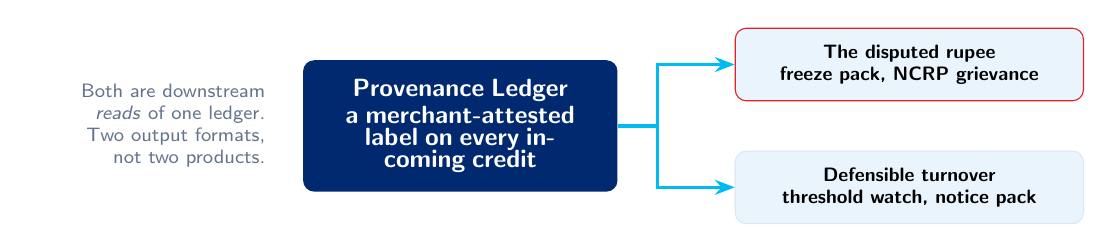
\begin{tikzpicture}[font=\scriptsize]
\node[rounded corners=4pt,fill=navy,text=white,inner sep=7pt,align=center,text width=3.5cm]
  (eng) {\bfseries\small Provenance Ledger\\[0.15em] a merchant-attested label on every incoming credit};
\node[rounded corners=4pt,fill=tint,draw=bad,inner sep=6pt,align=center,text width=4.0cm]
  (tax) at ($(eng.east)+(3.7,0.78)$) {\bfseries The disputed rupee\\ freeze pack, NCRP grievance};
\node[rounded corners=4pt,fill=tint,draw=hairline,inner sep=6pt,align=center,text width=4.0cm]
  (fra) at ($(eng.east)+(3.7,-0.78)$) {\bfseries Defensible turnover\\ threshold watch, notice pack};
\draw[-{Stealth[length=2.5mm]},ptmcyan,line width=1.3pt] (eng.east) -- ++(0.5,0) |- (tax.west);
\draw[-{Stealth[length=2.5mm]},ptmcyan,line width=1.3pt] (eng.east) -- ++(0.5,0) |- (fra.west);
\node[anchor=east,text width=2.9cm,align=right,text=muted] at ($(eng.west)+(-0.35,0)$)
  {Both are downstream \emph{reads} of one ledger. Two output formats, not two products.};
\end{tikzpicture}
\end{center}
\vspace{0.1cm}
\begin{center}
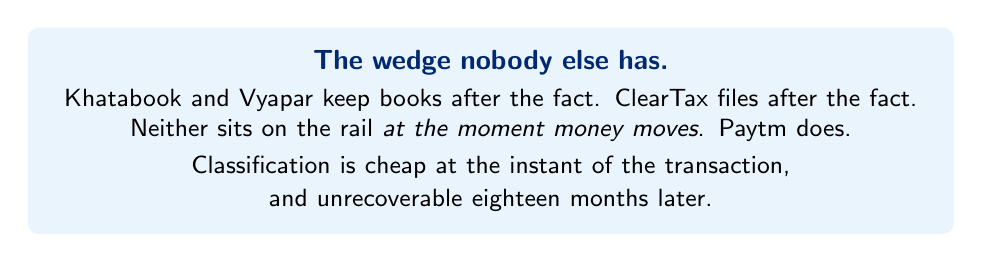
\begin{tikzpicture}\node[rounded corners=4pt,fill=tint,inner sep=8pt,text width=11.2cm,align=center]{
{\bfseries\color{navy}The wedge nobody else has.}\\[0.25em]
\small Khatabook and Vyapar keep books after the fact. ClearTax files after the fact.\\
Neither sits on the rail \emph{at the moment money moves}. Paytm does.\\[0.25em]
\small Classification is cheap at the instant of the transaction,\\ and unrecoverable eighteen months later.
};\end{tikzpicture}
\end{center}
\note{{\color{navy}\bfseries\normalsize 6.~The insight}\par\vspace{0.55em}\textbf{0:40 --- why this is one product, not two.}
\\[0.4em]
Say: \emph{``Most teams would build the fraud tool or the tax tool. They are the
same engine.''} Both are downstream reads of one ledger --- two output formats,
and the freeze pack is the one we lead with.
\\[0.4em]
Then the wedge, and say it slowly because it is the defensible-moat answer:
Khatabook and Vyapar keep books after the fact, ClearTax files after the fact.
Neither sits on the rail at the moment money moves. \textbf{Paytm does.}
\\[0.4em]
Landing line: classification is cheap and accurate at the instant of the
transaction, and unrecoverable eighteen months later when the notice arrives.}
\end{frame}

% ============================================================ 7. THE ENGINE
\begin{frame}{The engine}{Eight tags, one tap}
\vspace{0.15cm}
\begin{columns}[T]
\begin{column}{0.45\textwidth}
{\color{navy}\bfseries\small Every incoming credit gets one tag}\\[0.4em]
{\scriptsize
\begin{tabular}{@{}ll@{}}
\texttt{taxable\_supply}    & ordinary sale \\
\texttt{exempt\_supply}     & vegetables, milk, loose rice \\
\texttt{personal\_transfer} & spouse, parent, sibling \\
\texttt{inter\_account}     & her own money \\
\texttt{refund\_reversal}   & money back from a vendor \\
\texttt{duplicate}          & paid twice, one refunded \\
\texttt{non\_business}      & loan, chit payout, gift \\
{\color{bad}\texttt{unclassified}} & {\color{bad}not enough signal: ask her} \\
\end{tabular}}
\\[0.75em]
{\scriptsize\color{muted}98.6\% are ordinary sales, settled by rules. The agent reasons only about the 1.4\% that need judgement.}
\end{column}
\begin{column}{0.51\textwidth}
\card{6.6cm}{{\bfseries\color{navy}The agent proposes. The merchant attests.}\\[0.4em]
\scriptsize You cannot infer \qm{my husband sent this} from a QR payment. The agent proposes a tag \emph{with its reason}; she confirms with one tap, in Kannada, batched daily.\\[0.45em]
\scriptsize Not a fallback. A ledger she attested \emph{at the time} survives a hearing. An algorithm's guess, made under duress a year later, does not.}
\\[0.55em]
\hspace{0.15cm}\begin{minipage}{6.6cm}
{\bfseries\color{navy}\small Budget: at most 3 questions a day.}\\[0.15em]
{\scriptsize\color{muted}Over a simulated year: \hi{189 questions, median 1.3 a day}. Ask more and the product is dead.}
\end{minipage}
\end{column}
\end{columns}
\note{{\color{navy}\bfseries\normalsize 7.~The engine}\par\vspace{0.55em}\textbf{0:45 --- the mechanism. Do not read the tag list.}
\\[0.4em]
Gesture at the eight tags, say ``eight labels, every incoming credit gets one,''
and move to the right-hand card, which is the real content.
\\[0.4em]
\textbf{The line that matters:} you cannot infer ``my husband sent this'' from a
QR payment. So the agent proposes a tag \emph{with its reason} and she confirms
with one tap. This is not a fallback --- a ledger she attested contemporaneously
survives a hearing; an algorithm's guess produced under duress a year later does not.
\\[0.4em]
Then the budget: at most three questions a day, and we measured 189 across a
year, median 1.3. Ask more than that and the product is dead.
\\[0.4em]
If asked about cost: 98.6\% are ordinary sales settled by rules. The model only
sees the 1.4\% that need judgement.}
\end{frame}

% ============================================================ 8. PRODUCT
\begin{frame}{What the merchant sees}
\vspace{-0.1cm}
\begin{center}
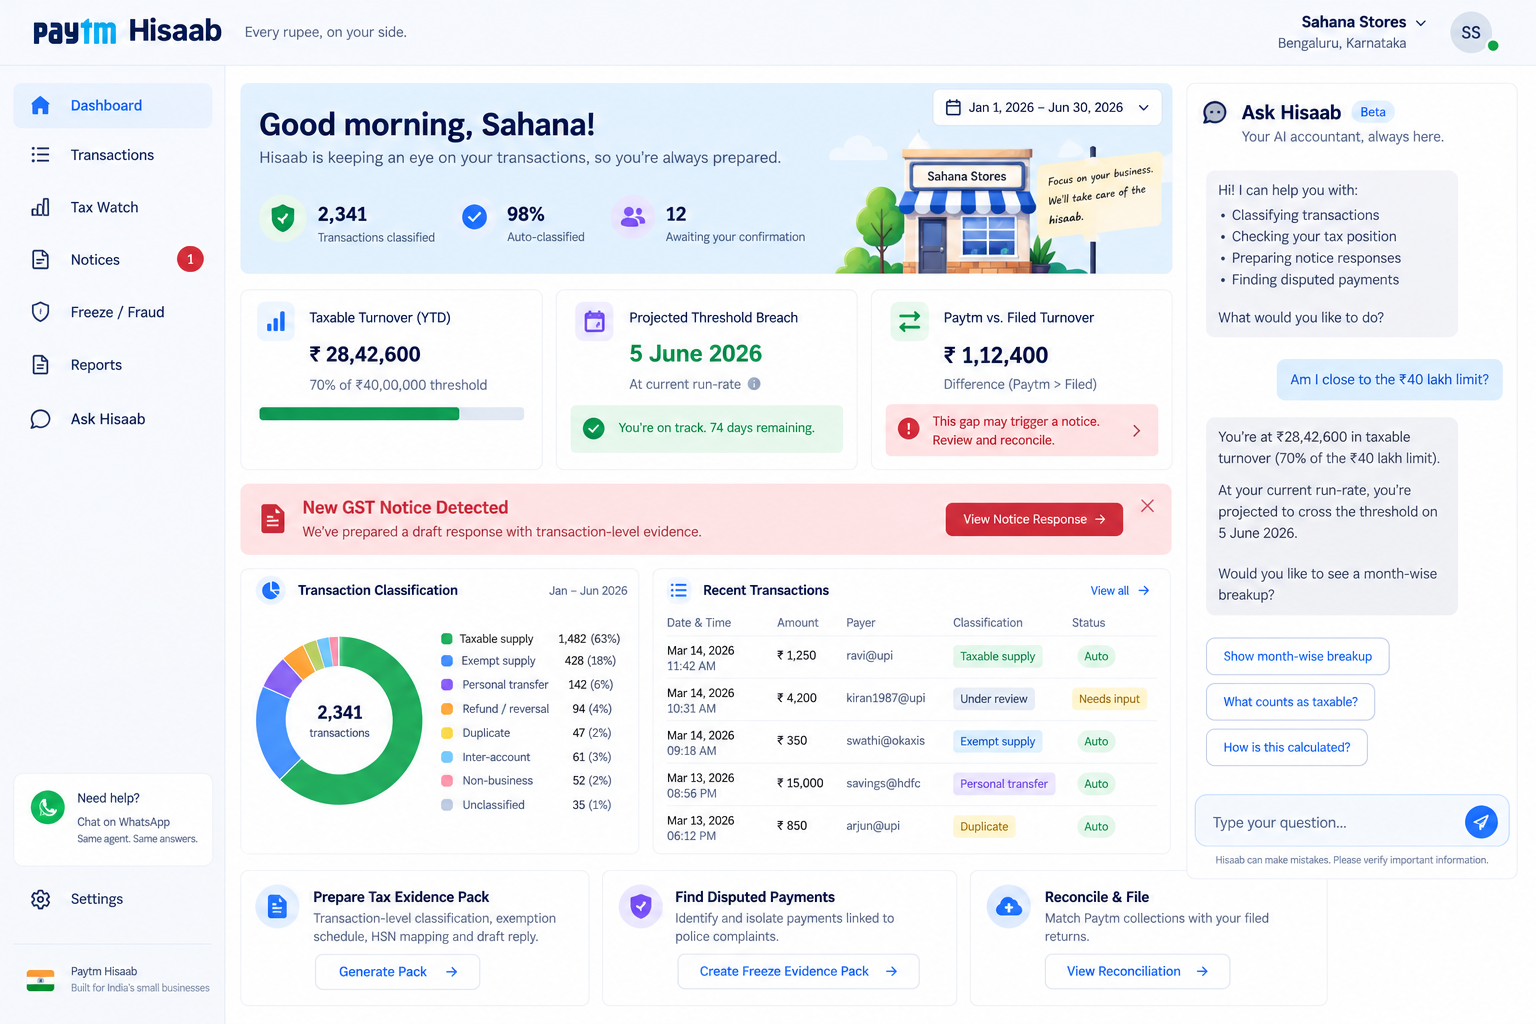
\includegraphics[width=\textwidth,height=0.70\textheight,keepaspectratio]{Paytm-Hisaab_website_look.png}
\end{center}
\vspace{0.1cm}
\hspace{0.05cm}{\scriptsize\color{muted}One surface: what every payment was classified as, how close she is to the threshold, and the packs. The same agent runs on WhatsApp, where she actually is.}
\note{{\color{navy}\bfseries\normalsize 8.~What the merchant sees}\par\vspace{0.55em}\textbf{0:20 --- a glance slide. Do not tour the UI.}
\\[0.4em]
One sentence: everything classified, how close she is to the threshold, and the
packs, on one surface.
\\[0.4em]
Then the WhatsApp point --- the same agent, where she actually is --- and advance.
\\[0.4em]
If someone asks whether this is built: the chat and the tools are live; this
screen is the product surface we are designing toward.}
\end{frame}

% ============================================================ 9. ARCHITECTURE
\begin{frame}{Built on Phinite}{Two agent graphs, four agents, ten deterministic skills}
\vspace{0.15cm}
\begin{columns}[T]
\begin{column}{0.53\textwidth}
{\scriptsize
\begin{tabular}{@{}L{1.75cm}L{4.7cm}@{}}
\multicolumn{2}{@{}l}{\color{navy}\bfseries\small hisaab-watch \;\scriptsize(autonomous: cron + API)}\\
\midrule
Provenance & proposes a tag and a reason for the hard credits \\
Evidence   & assembles packs: freeze evidence, then exemption schedules and HSN \\
\addlinespace[0.6em]
\multicolumn{2}{@{}l}{\color{navy}\bfseries\small hisaab-merchant \;\scriptsize(conversational: chat)}\\
\midrule
Merchant   & the conversation: attestation, alerts, Kannada \\
Escalation & decides when to stop and route to a human CA \\
\bottomrule
\end{tabular}}
\\[0.75em]
{\scriptsize\color{muted}The nightly pass writes its queue to the ledger; the chat reads it when she opens it. Deliberately \emph{not} a graph-to-graph call: a queue that outlives either run is what makes the handoff robust.}
\end{column}
\begin{column}{0.44\textwidth}
\card{5.7cm}{{\bfseries\color{navy}Permissions are the product}\\[0.4em]
\scriptsize Provenance proposes, \red{never commits}.\\[0.25em]
\scriptsize Merchant is the \emph{only} agent that can commit a tag.\\[0.25em]
\scriptsize Evidence is \red{read-only}. It cannot edit a classification to make a pack look better.\\[0.25em]
\scriptsize Escalation can \red{halt} any pack; a human approves.}
\\[0.5em]
\hspace{0.1cm}\begin{minipage}{5.7cm}{\scriptsize\color{muted}Ten tools run live against a hosted service. Every number in a pack traces back, in the trace, to the credit and the attestation behind it.}\end{minipage}
\end{column}
\end{columns}
\note{{\color{navy}\bfseries\normalsize 9.~Built on Phinite}\par\vspace{0.55em}\textbf{0:40 --- for the technical judges.}
\\[0.4em]
Two agent graphs, not four loose agents: \texttt{hisaab-watch} runs autonomously on
cron, \texttt{hisaab-merchant} is the conversation. The nightly pass writes a queue;
the chat reads it when she opens it --- deliberately not a graph-to-graph call,
because a queue that outlives either run is what makes the handoff robust.
\\[0.4em]
\textbf{Spend your time on the right-hand card.} The strongest line in it:
the Evidence agent is read-only --- \emph{the agent that builds the defence cannot
edit the evidence.} And only the Merchant agent can commit an attested tag.
\\[0.4em]
Those are enforced as Phinite tool policies, not conventions, and a denied call
shows up in the trace.}
\end{frame}

% ============================================================ 10. DESIGN DECISIONS
\begin{frame}{Four decisions that make it defensible}
\vspace{0.3cm}
\begin{columns}[T]
\begin{column}{0.48\textwidth}
\card{6.0cm}{{\bfseries\color{navy}1. Arithmetic lives in skills, not the model}\\[0.35em]
\scriptsize Turnover, projections and apportionment are deterministic Python: versioned, testable, traceable. Wrapping arithmetic in an LLM is the standard tell, and the trace would show it.}
\\[0.35em]
\card{6.0cm}{{\bfseries\color{navy}3. Refusing to guess is a feature}\\[0.35em]
\scriptsize An \texttt{unclassified} credit routed to the merchant costs one tap. A confident wrong tag inside an evidence pack is a catastrophe. We report the refusal rate honestly.}
\end{column}
\begin{column}{0.48\textwidth}
\card{6.0cm}{{\bfseries\color{navy}2. Attestation is the promotion boundary}\\[0.35em]
\scriptsize Nothing enters a production pack that the merchant has not confirmed. Sandbox to UAT to prod, with her tap as the gate.}
\\[0.35em]
\card{6.0cm}{{\bfseries\color{navy}4. Ground truth, so accuracy is a number}\\[0.35em]
\scriptsize We simulated a year of a shop's life from a known process, split into what Paytm can see and what really happened. Agents read only the visible half, which is why we quote error bars instead of vibes.}
\end{column}
\end{columns}
\note{{\color{navy}\bfseries\normalsize 10.~Four decisions}\par\vspace{0.55em}\textbf{0:35 --- the slide that separates you from a demo.}
\\[0.4em]
Lead with \#1: all arithmetic is deterministic Python, not model output. Wrapping
arithmetic in an LLM is the standard tell, and the trace would show it.
\\[0.4em]
Then \#3: refusing to guess is a feature. An \texttt{unclassified} credit costs one
tap; a confident wrong tag inside an evidence pack is a catastrophe.
\\[0.4em]
Skim \#2 and \#4 --- one clause each. \#4 is worth a beat if the room is technical:
we generated ground truth, so accuracy is a number instead of a claim.}
\end{frame}

% ============================================================ 11. DEMO / ATTESTATION
\begin{frame}{Demo $\cdot$ Sahana Stores, Jayanagar}{An ordinary Tuesday, before anything goes wrong}
\vspace{0.1cm}
\begin{columns}[T]
\begin{column}{0.48\textwidth}
{\scriptsize\color{muted}Tuesday 10 March. Thirty-nine credits came in over the weekend. The agent asks about \hi{three}.}
\\[0.4em]
\card{5.9cm}{{\kn\scriptsize ಭಾನುವಾರ ರಾತ್ರಿ ₹15,000. ನಿಮ್ಮ ಸ್ವಂತ ಹಣವೇ?}\\[0.25em]
{\color{muted}\scriptsize \qm{₹15,000 at 11:04pm Sunday, from your savings account. Your own money?}}\\[0.35em]
{\scriptsize\color{navy}\fbox{\kn ಹೌದು}\;\fbox{\kn ಇಲ್ಲ}}}
\\[0.4em]
{\scriptsize $\cdot$\; ₹7,500 from her husband, scanned at the shop QR\\[0.25em]
$\cdot$\; ₹4,850 from Raghu Shetty, who has bought twice before. A real sale, and the agent \emph{asks} rather than assumes.}
\\[0.4em]
{\scriptsize\color{muted}The other thirty-six settle silently, and a ₹23 payment nobody can place is left alone.}
\end{column}
\begin{column}{0.48\textwidth}
\ocard{amber}{6.1cm}{{\bfseries\color{amber}And yes, two of those three should not be there}\\[0.35em]
\scriptsize A business QR is not for personal money, and the terms say so. It arrives anyway: family, own top-ups, a chit payout. The rule does not prevent it. It only means \emph{nobody keeps a record of it.}}
\\[0.45em]
{\scriptsize Paytm already reads the signals: channel, linked VPAs, payer history. What no system has is the \hi{merchant's own answer}, given at the time, in her language, and kept.}
\\[0.45em]
{\scriptsize That record is what the next two slides are built from: first for the police, then for the department.}
\end{column}
\end{columns}
\note{{\color{navy}\bfseries\normalsize 11.~Demo --- an ordinary Tuesday (beat 1)}\par\vspace{0.55em}\textbf{0:45 --- or hand over to the live demo here.}
\\[0.4em]
Thirty-nine credits came in over the weekend, the agent asks about \textbf{three}.
Read the Kannada line if you can; otherwise read the gloss under it.
\\[0.4em]
\textbf{Do not hide from the right-hand card --- lead with it.} The mid-review
point was that personal money is not allowed on a business QR. Correct, and we say
so on the slide. The argument is that the rule does not stop it, it only means no
one records it, and an unrecorded credit is what an authority later reads as income.
\\[0.4em]
\textbf{Second half of that card matters just as much.} We are not claiming Paytm
does nothing. It already reads channel, linked VPAs and payer history. What no
system has is her own answer, captured while it is still knowable. That is the
product, and it is a smaller, truer claim than the one we started with.
\\[0.4em]
\textbf{Before going on stage:} confirm the attestation queue is whole ---
\texttt{pending\_total} must be 3. A rehearsal that taps through this beat spends the
queue, and Render needs a clear-cache redeploy to restore it.}
\end{frame}

% ============================================================ 12. DEMO / THE FREEZE
\begin{frame}{Demo $\cdot$ The emergency}{The account is frozen at 09:30 and the supplier payment is due}
\vspace{0.2cm}
\begin{columns}[T]
\begin{column}{0.46\textwidth}
{\scriptsize She sold someone 12kg of onions. That customer was three layers downstream of a fraud victim. She is not named in the FIR, which was filed in another state, and \hi{339 payments} came in that week.}
\\[0.5em]
\card{5.8cm}{{\bfseries\color{navy}The agent isolates it}\\[0.35em]
\scriptsize ₹4,200 on 21 March at 19:47, till POS01. Matched by UTR \emph{and independently} by amount and date.\\[0.3em]
\scriptsize The sale record comes with it: the POS bill, the items, the till and the minute.}
\end{column}
\begin{column}{0.49\textwidth}
\ocard{amber}{6.1cm}{{\bfseries\color{amber}And the decoy it did not choose}\\[0.35em]
\scriptsize A \emph{second} ₹4,200 that same week, from a regular customer. Listed in the pack, and explicitly \emph{not} named as the disputed one. Only the date separates them.}
\\[0.5em]
{\scriptsize Then it drafts the NCRP-CFCFRMS grievance, citing the judgments that only the \emph{disputed amount} should be lien-marked, not the whole account.}
\\[0.5em]
{\scriptsize\color{bad}\bfseries It never asserts that she is innocent.}\\[0.1em]
{\scriptsize\color{muted}Some frozen accounts genuinely are mule accounts. The agent assembles evidence; a human decides. Escalation holds the pack for approval.}
\end{column}
\end{columns}
\note{{\color{navy}\bfseries\normalsize 12.~Demo --- the emergency (beat 4)}\par\vspace{0.55em}\textbf{0:50 --- this is now the lead case. Give it the most time of the three.}
\\[0.4em]
Set the stakes in one sentence: account frozen at half nine, supplier payment due,
339 payments came in that week, and she is not named in the FIR.
\\[0.4em]
\textbf{Why this one leads.} She did nothing wrong and there is no rule she broke.
She sold onions to a customer who turned out to be laundering. Every objection
available against the tax case --- she should not have taken personal money on that
QR, she should have registered --- has no purchase here at all.
\\[0.4em]
The agent isolates ₹4,200 by UTR \emph{and independently} by amount and date, and
brings the POS bill with it --- the items, till POS01, 19:47.
\\[0.4em]
\textbf{The decoy is the point.} A second ₹4,200 that same week from a regular
customer, listed in the pack and explicitly not chosen. Anyone can match an amount;
the pack shows its work.
\\[0.4em]
Finish on the red line: it never asserts she is innocent. Some frozen accounts
genuinely are mule accounts. We assemble evidence; a human decides, and Escalation
holds the pack for approval.}
\end{frame}

% ============================================================ 13. DEMO / TAX
\begin{frame}{Demo $\cdot$ The warning, and the notice}{The same ledger, read for the other authority}
\vspace{0.15cm}
\begin{columns}[T]
\begin{column}{0.38\textwidth}
{\scriptsize\color{muted}Replayed as of 31 January:}
\\[0.35em]
\ocard{good}{4.8cm}{{\bfseries\color{ink}\scriptsize\qm{At your current rate you cross ₹40 lakh around {\color{bad}14 March}. You will need to register.}}\\[0.35em]
{\scriptsize\color{muted}\grn{43 days of warning}, and the date is computed, not typed.}}
\\[0.45em]
{\scriptsize\color{bad}\bfseries This beat is what makes the pitch safe.}\\[0.1em]
{\scriptsize\color{muted}Its first act on the tax side is telling her to register.}
\end{column}
\begin{column}{0.58\textwidth}
{\scriptsize\color{muted}Then the notice arrives, claiming {\color{bad}\bfseries ₹60.98L} of turnover:}
\\[0.3em]
{\scriptsize
\begin{tabular}{@{}lr@{\hskip 1.2em}l@{}}
\multicolumn{2}{@{}l}{\color{navy}\bfseries Aggregate turnover \quad ₹42.2L} & \sub{within \grn{1.6\%} of truth} \\
\midrule
Exempt supplies      & ₹31.3L & \sub{vegetables, loose rice} \\
Taxable supplies     & ₹10.9L & \sub{branded goods, oil, soap} \\
\addlinespace[0.45em]
\multicolumn{2}{@{}l}{\color{navy}\bfseries Not turnover at all \quad ₹18.8L} & \sub{every line traced} \\
\midrule
Her own accounts     & ₹7.4L & \sub{top-ups before supplier runs} \\
Family               & ₹6.1L & \sub{spouse, parent, in-law} \\
Loans, chit, gifts   & ₹4.3L & \sub{chit payout, festival gifts} \\
Refunds, duplicates  & ₹1.0L & \sub{crate returns, double-taps} \\
\bottomrule
\end{tabular}}
\\[0.45em]
{\scriptsize And it says plainly: \hi{the claim is wrong, and you \emph{did} cross ₹40 lakh on 14 March. You must register.}}
\end{column}
\end{columns}
\note{{\color{navy}\bfseries\normalsize 13.~Demo --- the warning and the notice (beats 2 and 3)}\par\vspace{0.55em}\textbf{0:50 --- two tax beats on one slide, deliberately compressed.}
\\[0.4em]
Left: replayed as of 31 January, the agent says she crosses ₹40 lakh around
14 March. \textbf{Say the red line out loud} --- its first act on the tax side is
telling her she owes a registration. That is what stops the room turning hostile.
\\[0.4em]
Right: the notice claims ₹60.98 lakh, and the pack answers it line by line, every
figure traceable to transaction IDs. Then the honest half:
\textbf{the claim is wrong, and she did cross ₹40 lakh, and she must register.}
\\[0.4em]
\textbf{If a judge diffs this against slide 5:} slide 5 shows seeded truth
(₹42.9L), this shows what our system computed (₹42.2L). The 1.6\% between them
\emph{is} the accuracy claim --- say that, do not hedge.
\\[0.4em]
\textbf{If pushed on the personal and own-account lines:} same answer as slide 11.
Those credits should not be on a business QR, they are there anyway, and the
alternative to classifying them is letting them be read as income.}
\end{frame}

% ============================================================ 14. NUMBERS
\begin{frame}{What we can actually prove}{One merchant, one year, 13,267 credits, scored against seeded truth}
\vspace{0.45cm}
\begin{columns}[T]
\begin{column}{0.33\textwidth}
\begin{center}\bignum{1.6\%}{error on aggregate turnover\\ (taxable share within 1\%)}\end{center}
\vspace{0.55cm}
\begin{center}\bignum{43 days}{of warning before the\\ threshold crossing}\end{center}
\end{column}
\begin{column}{0.33\textwidth}
\begin{center}\bignum{1.3 a day}{median questions asked.\\ 189 in a year, never over 3}\end{center}
\vspace{0.55cm}
\begin{center}\bignum{zero}{credits left untagged\\ across the whole year}\end{center}
\end{column}
\begin{column}{0.30\textwidth}
\card{3.8cm}{{\bfseries\color{navy}The honest baseline}\\[0.35em]
\scriptsize A 50-line rules-only classifier gets 99.3\% on sale vs not-a-sale, but catches only \red{77.8\%} of non-sale credits.\\[0.3em]
\scriptsize That residue alone puts two eval merchants on the \emph{wrong side} of ₹40L.\\[0.3em]
\scriptsize Closing it is what the agent plus one tap is for.}
\end{column}
\end{columns}
\vspace{0.45cm}
\hspace{0.1cm}{\scriptsize\color{muted}She corrected the agent 52 times that year. Those corrections are the ledger's strongest evidence, not its failures.}
\note{{\color{navy}\bfseries\normalsize 14.~What we can actually prove}\par\vspace{0.55em}\textbf{0:30 --- do not read all four. Pick two.}
\\[0.4em]
Lead with \textbf{1.6\%} error on turnover and \textbf{1.3 questions a day}. The
other two are there to be read, not narrated.
\\[0.4em]
\textbf{The credibility move is the box on the right} --- volunteer the weakness
before anyone finds it. A rules-only baseline gets 99.3\% on sale vs not-a-sale
but catches only 77.8\% of non-sale credits, and that residue alone puts two eval
merchants on the wrong side of ₹40 lakh. Closing it is what the agent plus one tap is for.
\\[0.4em]
Last line if you have the beat: she corrected the agent 52 times that year, and
those corrections are the ledger's strongest evidence, not its failures.}
\end{frame}

% ============================================================ 15. CLOSE
\begin{frame}{The line we do not cross}{Accuracy, not minimisation}
\vspace{0.3cm}
\begin{columns}[T]
\begin{column}{0.52\textwidth}
{\scriptsize
$\cdot$\; We \hi{never assert innocence} on a freeze. Some accounts really are mule accounts. We assemble evidence; a human decides.\\[0.5em]
$\cdot$\; We \hi{file nothing} with any authority. Artefacts only; the merchant or their CA files.\\[0.5em]
$\cdot$\; We compute what she \hi{genuinely owes} and say so plainly, including \qm{you crossed the threshold, you must register.}\\[0.5em]
$\cdot$\; We \hi{never assert a final liability}. We compute, show the workings, and route to a CA.\\[0.5em]
$\cdot$\; A business QR is \hi{not for personal money}. We do not excuse it. We record it, so it is not read as income.}
\end{column}
\begin{column}{0.44\textwidth}
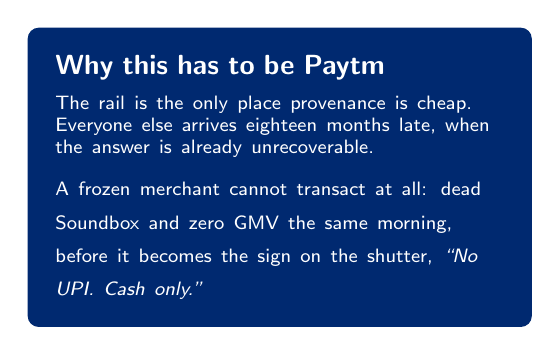
\begin{tikzpicture}\node[rounded corners=4pt,fill=navy,text=white,inner sep=10pt,text width=5.7cm,align=left]{
{\bfseries Why this has to be Paytm}\\[0.45em]
\scriptsize The rail is the only place provenance is cheap. Everyone else arrives eighteen months late, when the answer is already unrecoverable.\\[0.45em]
\scriptsize A frozen merchant cannot transact at all: dead Soundbox and zero GMV the same morning, before it becomes the sign on the shutter, \emph{\qm{No UPI. Cash only.}}
};\end{tikzpicture}
\end{column}
\end{columns}
\vspace{0.4cm}
\begin{center}
{\large\color{navy}\bfseries Paytm Hisaab}\quad{\color{muted}every rupee, on your side.}
\end{center}
\note{{\color{navy}\bfseries\normalsize 15.~The line we do not cross}\par\vspace{0.55em}\textbf{0:30 --- the non-negotiables, fast, then land.}
\\[0.4em]
Run the five bullets at pace. The one to hit is the first: we never assert
innocence on a freeze. The last is the mid-review answer, on the slide on purpose.
\\[0.4em]
Then the navy box: provenance is cheap only on the rail, and a frozen merchant
stops transacting the same morning.
\\[0.4em]
Final line, unhurried: \emph{``Paytm Hisaab. Every rupee, on your side.''} Stop talking.
\\[0.5em]
{\scriptsize
{\color{navy}\bfseries --- Q\&A prep ---}
\\[0.3em]
\textbf{``Merchants may not take personal money on a business QR.''} Correct, and
slide 11 says so before you have to. It arrives anyway, and the alternative to
recording it is letting an authority read it as income. We are not defending the
behaviour --- we are refusing to let it become a liability.
\\[0.3em]
\textbf{``Paytm already tags transactions.''} It does, and we build on that rather
than around it: channel, linked VPAs and payer history feed the rules layer. What
no tag carries is her attestation --- the part an authority accepts, and the only
part she alone can give.
\\[0.3em]
\textbf{``No return mismatch?''} That check needs a \emph{registered} composition
dealer who filed a CMP-08 to disagree with. Ours is unregistered, which is why she
gets a notice at all; the eval split has one with four quarters seeded.
\\[0.3em]
\textbf{``Exempt vs taxable on a QR sale?''} Not per payment. We apportion by value
from that shop's own POS-billed ratio and label it an estimate. Labelling each sale
by its majority side understated taxable turnover threefold.
\\[0.3em]
\textbf{``Four LLM calls in a trenchcoat?''} Everything deterministic is a skill and
four agents is the ceiling. If twenty lines of Python replaces an agent, it should
have been a skill --- the trace shows which is which.
\\[0.3em]
\textbf{``No standing with the police.''} Agreed: Paytm supplies, the merchant
files. By design. Cash sales are real, out of scope, and on the slide.}}
\end{frame}

\end{document}
"
\ifdefined\shownotes
  \setbeamertemplate{note page}{%
    \usebeamercolor[fg]{normal text}%
    \vspace{0.2em}%
    {\scriptsize\color{muted}Paytm Hisaab \;$\cdot$\; speaker notes}\hfill
    {\scriptsize\color{muted}slide \insertframenumber\ of 15}\par
    \vspace{0.25em}{\color{ptmcyan}\rule{\textwidth}{1.5pt}}\par
    \vspace{0.55em}\footnotesize\raggedright\insertnote\par}
  \setbeameroption{show only notes}
\fi

\begin{document}

% ============================================================ 1. TITLE
{\setbeamertemplate{footline}{}
\begin{frame}[plain]
\vspace{0.9cm}
\begin{center}
{\fontsize{38}{42}\selectfont\bfseries\color{navy}Paytm\;\color{ink}Hisaab}\\[0.45em]
{\Large\color{muted}Every rupee, on your side.}\\[0.9em]
{\color{ptmcyan}\rule{2.8cm}{2.5pt}}\\[0.9em]
{\large\color{ink}The agent that lets a merchant account for their own money}\\[0.15em]
{\large\color{ink}when someone in authority demands an explanation.}\\[1.3em]
{\small\color{muted}Agent Labs Buildathon \;$\cdot$\; Phinite $\times$ Paytm \;$\cdot$\; Track 2: AI for Small Businesses}
\end{center}
\note{{\color{navy}\bfseries\normalsize 1.~Title}\par\vspace{0.55em}\textbf{0:10 --- open cold.} Do not read the title or the tagline off the slide.
\\[0.4em]
Say: \emph{``I want to tell you about a man in Haveri who opened an envelope.''} Then advance.
\\[0.4em]
Nothing on this slide needs explaining. The tagline lands at the end, not here.}
\end{frame}}

% ============================================================ 2. STORY
\begin{frame}{Haveri, 2025}{A vegetable vendor opens an envelope}
\vspace{0.05cm}
\begin{columns}[T]
\begin{column}{0.52\textwidth}
\vspace{0.15cm}
He sells vegetables. Vegetables are \hi{exempt} from GST.\\[0.6em]
He also took UPI, because Paytm asked him to.\\[0.6em]
Four years of credits into his account, added up and billed as income:
\begin{center}\vspace{0.1em}{\fontsize{30}{32}\selectfont\bfseries\color{bad}₹29 lakh}\end{center}
\end{column}
\begin{column}{0.44\textwidth}
\ocard{hairline}{5.4cm}{\centering
  {\color{muted}\scriptsize Within weeks, on shutters across Karnataka:}\\[0.6em]
  {\fontsize{20}{23}\selectfont\bfseries\color{ink}\qm{No UPI.\\ Cash only.}}\\[0.6em]
  {\color{muted}\scriptsize A statewide boycott, by the merchants who had just adopted it.}}
\end{column}
\end{columns}
\vspace{0.25cm}
\hspace{0.1cm}{\small\sub{Withdrawn for the traders who could \emph{show} what they sold. Most could not. And tax is no longer the only authority asking.}}
\note{{\color{navy}\bfseries\normalsize 2.~Haveri, 2025}\par\vspace{0.55em}\textbf{0:45 --- the hook. Tell it, do not summarise it.}
\\[0.4em]
Four beats, in this order: he sells vegetables; vegetables are exempt from GST;
he took UPI because \emph{we} asked him to; the department added up four years of
credits and sent him a bill for \textbf{₹29 lakh}.
\\[0.4em]
\textbf{Pause on the number.} Then the card: within weeks, shutters across Karnataka
read ``No UPI, cash only.'' Merchants we had just onboarded, boycotting the rail.
\\[0.4em]
Close on the bottom line --- the notices were withdrawn for traders who could
\emph{show} what they sold. Most could not. That verb is the whole product.
\\[0.4em]
\textbf{Then the bridge:} \emph{``and tax is no longer the only authority asking.''}
That sentence is doing the repositioning --- Haveri is not a tax story here, it is
the moment taking digital money became a liability. The sharper version of it is
two slides away.
\\[0.4em]
\textbf{Do not say this is happening right now.} It is 2025. The next slide is
what makes it current, and a judge who knows the episode will respect the distinction.}
\end{frame}

% ============================================================ 3. STILL HAPPENING
\begin{frame}{And this is not a 2025 story}{CAclubindia, last updated 02 September 2026: ten days ago}
\vspace{0.1cm}
\begin{center}

\includegraphics[width=12.4cm]{gst-notices-2026.png}
\end{center}
\vspace{0.35cm}
\card{13.1cm}{\scriptsize\qm{During August 2026, the GST Department issued a significant number of notices covering different financial years and involving a wide range of issues\ldots\ They covered matters such as ITC mismatches, ineligible credit, \hi{differences in turnover}, wrong GST classification or rate, \hi{exemption claims}, Reverse Charge Mechanism\ldots}}
\vspace{0.3cm}

\hspace{0.1cm}{\small Those two categories are the whole content of an evidence pack. And this is the \emph{slower} of the two authorities. The other one freezes the account first.}
\note{{\color{navy}\bfseries\normalsize 3.~And this is not a 2025 story}\par\vspace{0.55em}\textbf{0:25 --- fast. This slide exists to kill one objection.}
\\[0.4em]
Say: \emph{``That was last year. This was published ten days ago.''}
\\[0.4em]
Do not read the quote. Point at the two bolded phrases only ---
\textbf{differences in turnover} and \textbf{exemption claims} --- and say those
two categories are the entire content of what we build.
\\[0.4em]
\textbf{Land on the last line and move.} It is the handoff into the police
slide: this is the slower authority. The other one freezes first and asks
afterwards. Do not linger here --- tax is no longer the headline.}
\end{frame}

% ============================================================ 4. THE TRAP
\begin{frame}{Every rupee a merchant receives is now evidence}{Today it is only ever used against them}
\vspace{0.05cm}
\begin{columns}[T]
\begin{column}{0.47\textwidth}
\ocard{bad}{6.0cm}{{\bfseries\color{bad}The cyber-crime police}\\[0.35em]
\scriptsize Fraud money layers through accounts within minutes. The shop at the end of the chain, the one that sold someone a watermelon, is frozen. It did nothing wrong, is not named in the FIR, and finds out when a payment declines.}
\end{column}
\begin{column}{0.47\textwidth}
\card{6.1cm}{{\bfseries\color{navy}The tax department}\\[0.35em]
\scriptsize Compares UPI collections against filed returns and bills the difference. Registered traders too, with QR, wallet, card and cash deposits all in scope.}
\end{column}
\end{columns}
\vspace{0.4cm}
\begin{center}
{\large Both demand the same artefact: \hi{what was each rupee, actually?}}\\[0.3em]
{\small\color{muted}Paytm already sees more of this than anyone. What is missing is the \emph{merchant's own answer}, captured when it is still knowable.}
\end{center}
\vspace{0.15cm}
{\color{hairline}\hrule height 1pt}
\vspace{0.35em}
\hspace{0.05cm}{\scriptsize\bfseries\color{bad}What it costs Paytm:}~{\scriptsize a frozen merchant stops transacting that morning. A frightened one takes the QR down for good. Dead Soundbox, zero GMV, no lending origination.}
\note{{\color{navy}\bfseries\normalsize 4.~Every rupee is now evidence}\par\vspace{0.55em}\textbf{0:40 --- two authorities, one unanswerable question.}
\\[0.4em]
\textbf{Left card first and give it the time.} Fraud money layers within minutes,
and the shop at the end of the chain, \emph{the one that sold someone a watermelon},
gets frozen. It did nothing wrong, it is not named in the FIR, and it finds out
when a payment declines. Use the watermelon.
\\[0.4em]
Right card briskly: the department reconciles collections against filed returns
and bills the difference. One sentence, then move.
\\[0.4em]
Then the pivot: both demand the same artefact --- what was each rupee, actually.
\\[0.4em]
\textbf{Say the grey line as written.} We do \emph{not} claim Paytm does nothing
with this data --- it tags plenty. The gap is the merchant's own answer, captured
when it is still knowable. Claiming otherwise in this room gets corrected.
\\[0.4em]
\textbf{Slow down for the red line.} This is the business case, not a footnote:
a frozen merchant stops transacting that morning, a frightened one takes the QR
down for good. Dead Soundbox, zero GMV, no lending origination.}
\end{frame}

% ============================================================ 5. THE BAR
\begin{frame}{Gross credits are not turnover}{One shop, one year, ₹60.98 lakh of credits}
\vspace{0.1cm}
\begin{center}
\begin{tikzpicture}[x=1cm,y=1cm]
% --- what the notice counts
\node[anchor=west,font=\scriptsize\bfseries,text=bad] at (-0.05,1.80) {WHAT THE NOTICE COUNTS AS TURNOVER};
\fill[bad!85,rounded corners=2pt] (0,1.06) rectangle (11.4,1.60);
\node[font=\small\bfseries,text=white] at (5.7,1.33) {₹60.98 lakh};

% --- what actually happened   (1 lakh = 0.18696 cm, so the bars are the same length)
\node[anchor=west,font=\scriptsize\bfseries,text=navy] at (-0.05,0.66) {WHAT ACTUALLY HAPPENED};
\fill[good!80,rounded corners=2pt]  (0,-0.08)     rectangle (6.001,0.46);
\fill[good!45]                      (6.001,-0.08) rectangle (8.002,0.46);
\fill[ptmcyan!70]                   (8.002,-0.08) rectangle (9.385,0.46);
\fill[navy!55]                      (9.385,-0.08) rectangle (10.451,0.46);
\fill[amber!70]                     (10.451,-0.08)rectangle (11.255,0.46);
\fill[muted!60,rounded corners=2pt] (11.255,-0.08)rectangle (11.4,0.46);

% brackets
\draw[navy,line width=0.8pt] (0,-0.22) -- (0,-0.36) -- (8.002,-0.36) -- (8.002,-0.22);
\node[anchor=north,font=\scriptsize,text=navy,align=center] at (4.0,-0.38)
  {\bfseries ₹42.9L aggregate turnover\quad{\color{muted}\scriptsize exempt ₹32.1L + taxable ₹10.7L}};
\draw[bad,line width=0.8pt] (8.002,-0.22) -- (8.002,-0.36) -- (11.4,-0.36) -- (11.4,-0.22);
\node[anchor=north,font=\scriptsize,text=bad,align=center] at (9.7,-0.38)
  {\bfseries ₹18.1L that is not turnover at all};

% legend
\node[font=\scriptsize,text=ink] at (5.7,-1.02) {%
\textcolor{good!80}{$\blacksquare$}~Exempt sales \quad
\textcolor{good!45}{$\blacksquare$}~Taxable sales \quad
\textcolor{ptmcyan!70}{$\blacksquare$}~Her own accounts ₹7.4L};
\node[font=\scriptsize,text=ink] at (5.7,-1.40) {%
\textcolor{navy!55}{$\blacksquare$}~Family ₹5.7L \quad
\textcolor{amber!70}{$\blacksquare$}~Loans, chit, gifts ₹4.3L \quad
\textcolor{muted!60}{$\blacksquare$}~Refunds \& duplicates ₹0.7L};
\end{tikzpicture}
\end{center}
\vspace{0.15cm}
\hspace{0.1cm}{\small\sub{Personal money does not belong on a business QR. It arrives anyway, reads as turnover, and hides the one credit the police will ask about.}}
\note{{\color{navy}\bfseries\normalsize 5.~Gross credits are not turnover}\par\vspace{0.55em}\textbf{0:45 --- the hinge of the pitch. Let the picture work.}
\\[0.4em]
Say: \emph{``One shop, one year, ₹60.98 lakh of credits. The red bar is what the
notice counts as turnover --- all of it.''}
\\[0.4em]
Then the bottom bar. \textbf{Stop talking for two seconds} and let them read it.
\\[0.4em]
₹42.9L really is turnover, and we say so. ₹18.1L is not: her savings account, her
husband, a chit payout, a double-tap on the Soundbox.
\\[0.4em]
\textbf{Get in front of the obvious objection.} Personal money is not supposed to
touch a business QR. Say so first, then say it arrives anyway --- that is an
observation about merchants, not a loophole we are selling. The rule does not stop
it; it only means no one is keeping a record of it.
\\[0.4em]
\textbf{And close on the second use.} This volume is also why she cannot find the
one credit the police care about. Same bar, same problem, and the freeze slide
pays it off.
\\[0.4em]
If challenged on the numbers: seeded ground truth from our generator, not an
estimate. Accuracy against it is slide 14.}
\end{frame}

% ============================================================ 6. INSIGHT
\begin{frame}{The insight}{Most teams would build the tax tool \emph{or} the fraud tool. They are the same engine.}
\vspace{0.15cm}
\begin{center}
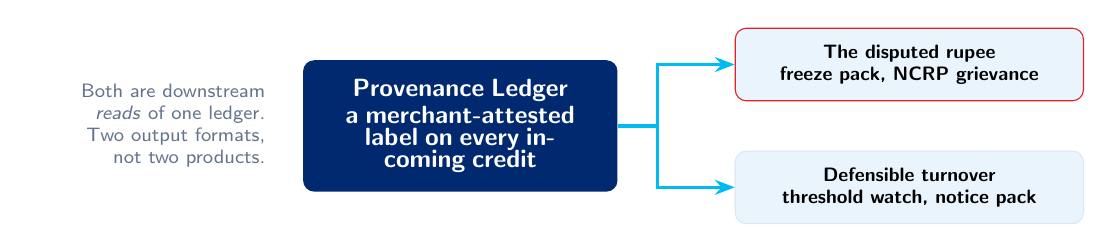
\begin{tikzpicture}[font=\scriptsize]
\node[rounded corners=4pt,fill=navy,text=white,inner sep=7pt,align=center,text width=3.5cm]
  (eng) {\bfseries\small Provenance Ledger\\[0.15em] a merchant-attested label on every incoming credit};
\node[rounded corners=4pt,fill=tint,draw=bad,inner sep=6pt,align=center,text width=4.0cm]
  (tax) at ($(eng.east)+(3.7,0.78)$) {\bfseries The disputed rupee\\ freeze pack, NCRP grievance};
\node[rounded corners=4pt,fill=tint,draw=hairline,inner sep=6pt,align=center,text width=4.0cm]
  (fra) at ($(eng.east)+(3.7,-0.78)$) {\bfseries Defensible turnover\\ threshold watch, notice pack};
\draw[-{Stealth[length=2.5mm]},ptmcyan,line width=1.3pt] (eng.east) -- ++(0.5,0) |- (tax.west);
\draw[-{Stealth[length=2.5mm]},ptmcyan,line width=1.3pt] (eng.east) -- ++(0.5,0) |- (fra.west);
\node[anchor=east,text width=2.9cm,align=right,text=muted] at ($(eng.west)+(-0.35,0)$)
  {Both are downstream \emph{reads} of one ledger. Two output formats, not two products.};
\end{tikzpicture}
\end{center}
\vspace{0.1cm}
\begin{center}
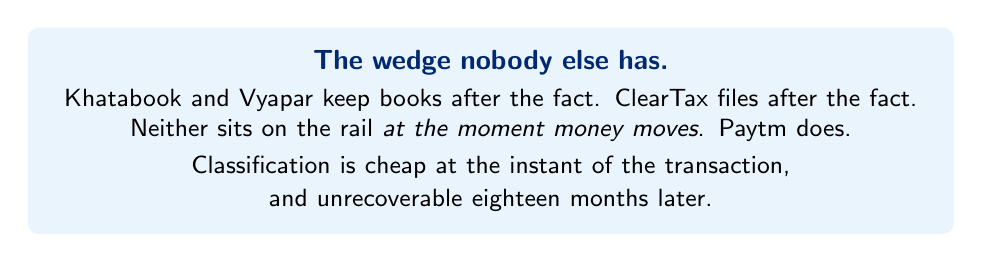
\begin{tikzpicture}\node[rounded corners=4pt,fill=tint,inner sep=8pt,text width=11.2cm,align=center]{
{\bfseries\color{navy}The wedge nobody else has.}\\[0.25em]
\small Khatabook and Vyapar keep books after the fact. ClearTax files after the fact.\\
Neither sits on the rail \emph{at the moment money moves}. Paytm does.\\[0.25em]
\small Classification is cheap at the instant of the transaction,\\ and unrecoverable eighteen months later.
};\end{tikzpicture}
\end{center}
\note{{\color{navy}\bfseries\normalsize 6.~The insight}\par\vspace{0.55em}\textbf{0:40 --- why this is one product, not two.}
\\[0.4em]
Say: \emph{``Most teams would build the fraud tool or the tax tool. They are the
same engine.''} Both are downstream reads of one ledger --- two output formats,
and the freeze pack is the one we lead with.
\\[0.4em]
Then the wedge, and say it slowly because it is the defensible-moat answer:
Khatabook and Vyapar keep books after the fact, ClearTax files after the fact.
Neither sits on the rail at the moment money moves. \textbf{Paytm does.}
\\[0.4em]
Landing line: classification is cheap and accurate at the instant of the
transaction, and unrecoverable eighteen months later when the notice arrives.}
\end{frame}

% ============================================================ 7. THE ENGINE
\begin{frame}{The engine}{Eight tags, one tap}
\vspace{0.15cm}
\begin{columns}[T]
\begin{column}{0.45\textwidth}
{\color{navy}\bfseries\small Every incoming credit gets one tag}\\[0.4em]
{\scriptsize
\begin{tabular}{@{}ll@{}}
\texttt{taxable\_supply}    & ordinary sale \\
\texttt{exempt\_supply}     & vegetables, milk, loose rice \\
\texttt{personal\_transfer} & spouse, parent, sibling \\
\texttt{inter\_account}     & her own money \\
\texttt{refund\_reversal}   & money back from a vendor \\
\texttt{duplicate}          & paid twice, one refunded \\
\texttt{non\_business}      & loan, chit payout, gift \\
{\color{bad}\texttt{unclassified}} & {\color{bad}not enough signal: ask her} \\
\end{tabular}}
\\[0.75em]
{\scriptsize\color{muted}98.6\% are ordinary sales, settled by rules. The agent reasons only about the 1.4\% that need judgement.}
\end{column}
\begin{column}{0.51\textwidth}
\card{6.6cm}{{\bfseries\color{navy}The agent proposes. The merchant attests.}\\[0.4em]
\scriptsize You cannot infer \qm{my husband sent this} from a QR payment. The agent proposes a tag \emph{with its reason}; she confirms with one tap, in Kannada, batched daily.\\[0.45em]
\scriptsize Not a fallback. A ledger she attested \emph{at the time} survives a hearing. An algorithm's guess, made under duress a year later, does not.}
\\[0.55em]
\hspace{0.15cm}\begin{minipage}{6.6cm}
{\bfseries\color{navy}\small Budget: at most 3 questions a day.}\\[0.15em]
{\scriptsize\color{muted}Over a simulated year: \hi{189 questions, median 1.3 a day}. Ask more and the product is dead.}
\end{minipage}
\end{column}
\end{columns}
\note{{\color{navy}\bfseries\normalsize 7.~The engine}\par\vspace{0.55em}\textbf{0:45 --- the mechanism. Do not read the tag list.}
\\[0.4em]
Gesture at the eight tags, say ``eight labels, every incoming credit gets one,''
and move to the right-hand card, which is the real content.
\\[0.4em]
\textbf{The line that matters:} you cannot infer ``my husband sent this'' from a
QR payment. So the agent proposes a tag \emph{with its reason} and she confirms
with one tap. This is not a fallback --- a ledger she attested contemporaneously
survives a hearing; an algorithm's guess produced under duress a year later does not.
\\[0.4em]
Then the budget: at most three questions a day, and we measured 189 across a
year, median 1.3. Ask more than that and the product is dead.
\\[0.4em]
If asked about cost: 98.6\% are ordinary sales settled by rules. The model only
sees the 1.4\% that need judgement.}
\end{frame}

% ============================================================ 8. PRODUCT
\begin{frame}{What the merchant sees}
\vspace{-0.1cm}
\begin{center}
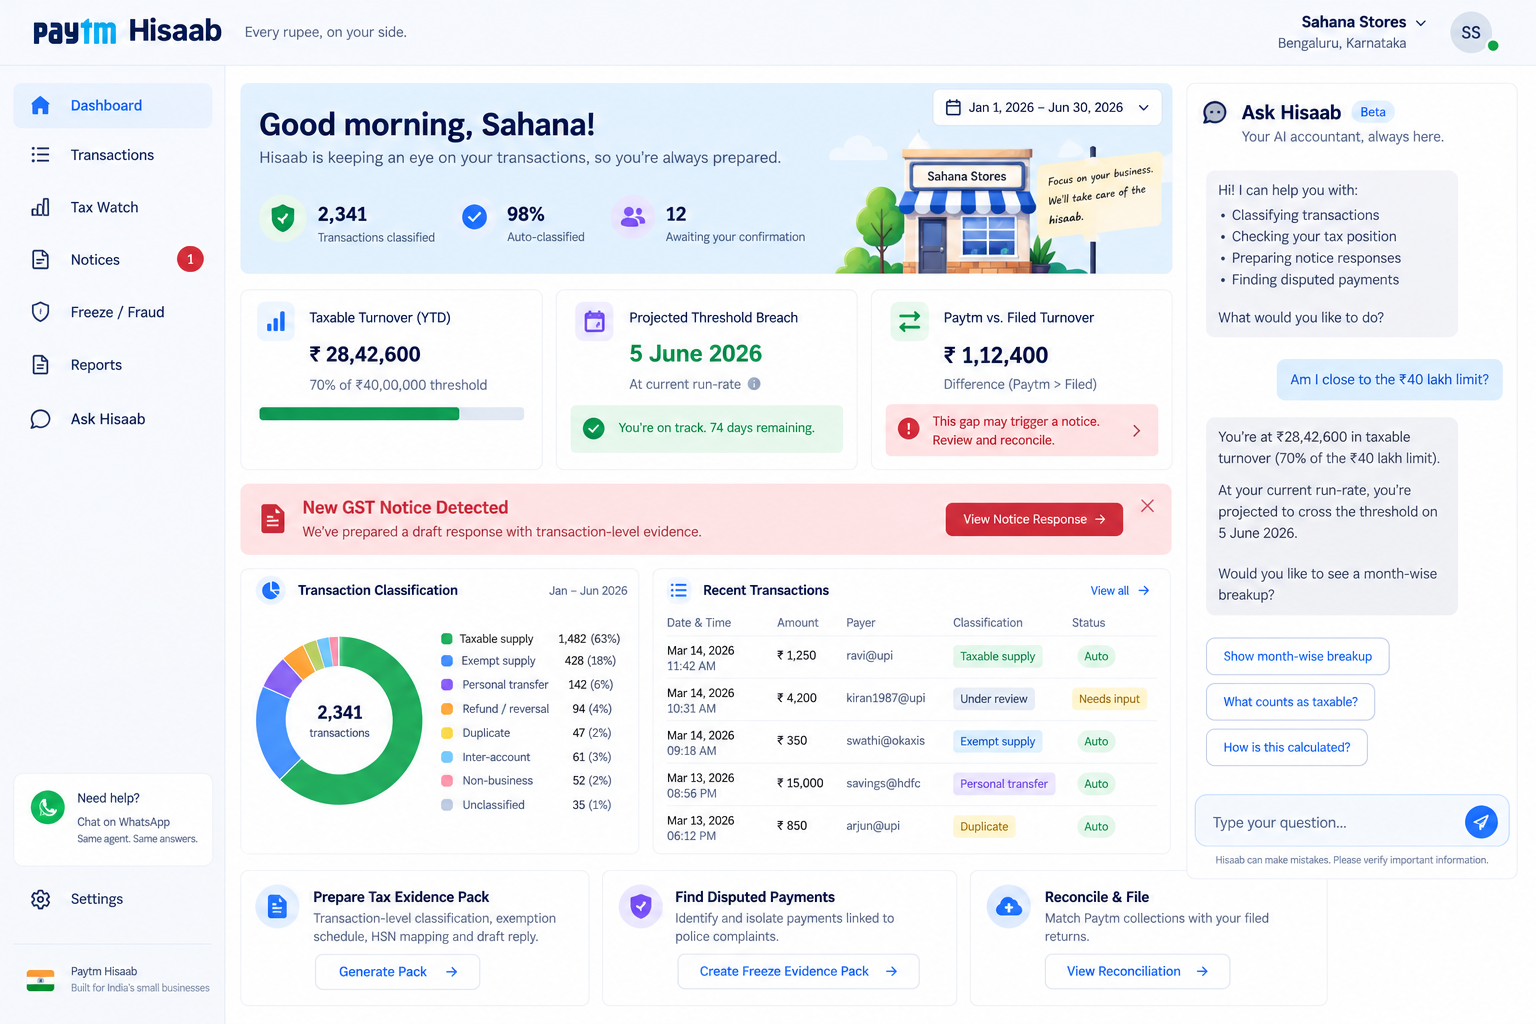
\includegraphics[width=\textwidth,height=0.70\textheight,keepaspectratio]{Paytm-Hisaab_website_look.png}
\end{center}
\vspace{0.1cm}
\hspace{0.05cm}{\scriptsize\color{muted}One surface: what every payment was classified as, how close she is to the threshold, and the packs. The same agent runs on WhatsApp, where she actually is.}
\note{{\color{navy}\bfseries\normalsize 8.~What the merchant sees}\par\vspace{0.55em}\textbf{0:20 --- a glance slide. Do not tour the UI.}
\\[0.4em]
One sentence: everything classified, how close she is to the threshold, and the
packs, on one surface.
\\[0.4em]
Then the WhatsApp point --- the same agent, where she actually is --- and advance.
\\[0.4em]
If someone asks whether this is built: the chat and the tools are live; this
screen is the product surface we are designing toward.}
\end{frame}

% ============================================================ 9. ARCHITECTURE
\begin{frame}{Built on Phinite}{Two agent graphs, four agents, ten deterministic skills}
\vspace{0.15cm}
\begin{columns}[T]
\begin{column}{0.53\textwidth}
{\scriptsize
\begin{tabular}{@{}L{1.75cm}L{4.7cm}@{}}
\multicolumn{2}{@{}l}{\color{navy}\bfseries\small hisaab-watch \;\scriptsize(autonomous: cron + API)}\\
\midrule
Provenance & proposes a tag and a reason for the hard credits \\
Evidence   & assembles packs: freeze evidence, then exemption schedules and HSN \\
\addlinespace[0.6em]
\multicolumn{2}{@{}l}{\color{navy}\bfseries\small hisaab-merchant \;\scriptsize(conversational: chat)}\\
\midrule
Merchant   & the conversation: attestation, alerts, Kannada \\
Escalation & decides when to stop and route to a human CA \\
\bottomrule
\end{tabular}}
\\[0.75em]
{\scriptsize\color{muted}The nightly pass writes its queue to the ledger; the chat reads it when she opens it. Deliberately \emph{not} a graph-to-graph call: a queue that outlives either run is what makes the handoff robust.}
\end{column}
\begin{column}{0.44\textwidth}
\card{5.7cm}{{\bfseries\color{navy}Permissions are the product}\\[0.4em]
\scriptsize Provenance proposes, \red{never commits}.\\[0.25em]
\scriptsize Merchant is the \emph{only} agent that can commit a tag.\\[0.25em]
\scriptsize Evidence is \red{read-only}. It cannot edit a classification to make a pack look better.\\[0.25em]
\scriptsize Escalation can \red{halt} any pack; a human approves.}
\\[0.5em]
\hspace{0.1cm}\begin{minipage}{5.7cm}{\scriptsize\color{muted}Ten tools run live against a hosted service. Every number in a pack traces back, in the trace, to the credit and the attestation behind it.}\end{minipage}
\end{column}
\end{columns}
\note{{\color{navy}\bfseries\normalsize 9.~Built on Phinite}\par\vspace{0.55em}\textbf{0:40 --- for the technical judges.}
\\[0.4em]
Two agent graphs, not four loose agents: \texttt{hisaab-watch} runs autonomously on
cron, \texttt{hisaab-merchant} is the conversation. The nightly pass writes a queue;
the chat reads it when she opens it --- deliberately not a graph-to-graph call,
because a queue that outlives either run is what makes the handoff robust.
\\[0.4em]
\textbf{Spend your time on the right-hand card.} The strongest line in it:
the Evidence agent is read-only --- \emph{the agent that builds the defence cannot
edit the evidence.} And only the Merchant agent can commit an attested tag.
\\[0.4em]
Those are enforced as Phinite tool policies, not conventions, and a denied call
shows up in the trace.}
\end{frame}

% ============================================================ 10. DESIGN DECISIONS
\begin{frame}{Four decisions that make it defensible}
\vspace{0.3cm}
\begin{columns}[T]
\begin{column}{0.48\textwidth}
\card{6.0cm}{{\bfseries\color{navy}1. Arithmetic lives in skills, not the model}\\[0.35em]
\scriptsize Turnover, projections and apportionment are deterministic Python: versioned, testable, traceable. Wrapping arithmetic in an LLM is the standard tell, and the trace would show it.}
\\[0.35em]
\card{6.0cm}{{\bfseries\color{navy}3. Refusing to guess is a feature}\\[0.35em]
\scriptsize An \texttt{unclassified} credit routed to the merchant costs one tap. A confident wrong tag inside an evidence pack is a catastrophe. We report the refusal rate honestly.}
\end{column}
\begin{column}{0.48\textwidth}
\card{6.0cm}{{\bfseries\color{navy}2. Attestation is the promotion boundary}\\[0.35em]
\scriptsize Nothing enters a production pack that the merchant has not confirmed. Sandbox to UAT to prod, with her tap as the gate.}
\\[0.35em]
\card{6.0cm}{{\bfseries\color{navy}4. Ground truth, so accuracy is a number}\\[0.35em]
\scriptsize We simulated a year of a shop's life from a known process, split into what Paytm can see and what really happened. Agents read only the visible half, which is why we quote error bars instead of vibes.}
\end{column}
\end{columns}
\note{{\color{navy}\bfseries\normalsize 10.~Four decisions}\par\vspace{0.55em}\textbf{0:35 --- the slide that separates you from a demo.}
\\[0.4em]
Lead with \#1: all arithmetic is deterministic Python, not model output. Wrapping
arithmetic in an LLM is the standard tell, and the trace would show it.
\\[0.4em]
Then \#3: refusing to guess is a feature. An \texttt{unclassified} credit costs one
tap; a confident wrong tag inside an evidence pack is a catastrophe.
\\[0.4em]
Skim \#2 and \#4 --- one clause each. \#4 is worth a beat if the room is technical:
we generated ground truth, so accuracy is a number instead of a claim.}
\end{frame}

% ============================================================ 11. DEMO / ATTESTATION
\begin{frame}{Demo $\cdot$ Sahana Stores, Jayanagar}{An ordinary Tuesday, before anything goes wrong}
\vspace{0.1cm}
\begin{columns}[T]
\begin{column}{0.48\textwidth}
{\scriptsize\color{muted}Tuesday 10 March. Thirty-nine credits came in over the weekend. The agent asks about \hi{three}.}
\\[0.4em]
\card{5.9cm}{{\kn\scriptsize ಭಾನುವಾರ ರಾತ್ರಿ ₹15,000. ನಿಮ್ಮ ಸ್ವಂತ ಹಣವೇ?}\\[0.25em]
{\color{muted}\scriptsize \qm{₹15,000 at 11:04pm Sunday, from your savings account. Your own money?}}\\[0.35em]
{\scriptsize\color{navy}\fbox{\kn ಹೌದು}\;\fbox{\kn ಇಲ್ಲ}}}
\\[0.4em]
{\scriptsize $\cdot$\; ₹7,500 from her husband, scanned at the shop QR\\[0.25em]
$\cdot$\; ₹4,850 from Raghu Shetty, who has bought twice before. A real sale, and the agent \emph{asks} rather than assumes.}
\\[0.4em]
{\scriptsize\color{muted}The other thirty-six settle silently, and a ₹23 payment nobody can place is left alone.}
\end{column}
\begin{column}{0.48\textwidth}
\ocard{amber}{6.1cm}{{\bfseries\color{amber}And yes, two of those three should not be there}\\[0.35em]
\scriptsize A business QR is not for personal money, and the terms say so. It arrives anyway: family, own top-ups, a chit payout. The rule does not prevent it. It only means \emph{nobody keeps a record of it.}}
\\[0.45em]
{\scriptsize Paytm already reads the signals: channel, linked VPAs, payer history. What no system has is the \hi{merchant's own answer}, given at the time, in her language, and kept.}
\\[0.45em]
{\scriptsize That record is what the next two slides are built from: first for the police, then for the department.}
\end{column}
\end{columns}
\note{{\color{navy}\bfseries\normalsize 11.~Demo --- an ordinary Tuesday (beat 1)}\par\vspace{0.55em}\textbf{0:45 --- or hand over to the live demo here.}
\\[0.4em]
Thirty-nine credits came in over the weekend, the agent asks about \textbf{three}.
Read the Kannada line if you can; otherwise read the gloss under it.
\\[0.4em]
\textbf{Do not hide from the right-hand card --- lead with it.} The mid-review
point was that personal money is not allowed on a business QR. Correct, and we say
so on the slide. The argument is that the rule does not stop it, it only means no
one records it, and an unrecorded credit is what an authority later reads as income.
\\[0.4em]
\textbf{Second half of that card matters just as much.} We are not claiming Paytm
does nothing. It already reads channel, linked VPAs and payer history. What no
system has is her own answer, captured while it is still knowable. That is the
product, and it is a smaller, truer claim than the one we started with.
\\[0.4em]
\textbf{Before going on stage:} confirm the attestation queue is whole ---
\texttt{pending\_total} must be 3. A rehearsal that taps through this beat spends the
queue, and Render needs a clear-cache redeploy to restore it.}
\end{frame}

% ============================================================ 12. DEMO / THE FREEZE
\begin{frame}{Demo $\cdot$ The emergency}{The account is frozen at 09:30 and the supplier payment is due}
\vspace{0.2cm}
\begin{columns}[T]
\begin{column}{0.46\textwidth}
{\scriptsize She sold someone 12kg of onions. That customer was three layers downstream of a fraud victim. She is not named in the FIR, which was filed in another state, and \hi{339 payments} came in that week.}
\\[0.5em]
\card{5.8cm}{{\bfseries\color{navy}The agent isolates it}\\[0.35em]
\scriptsize ₹4,200 on 21 March at 19:47, till POS01. Matched by UTR \emph{and independently} by amount and date.\\[0.3em]
\scriptsize The sale record comes with it: the POS bill, the items, the till and the minute.}
\end{column}
\begin{column}{0.49\textwidth}
\ocard{amber}{6.1cm}{{\bfseries\color{amber}And the decoy it did not choose}\\[0.35em]
\scriptsize A \emph{second} ₹4,200 that same week, from a regular customer. Listed in the pack, and explicitly \emph{not} named as the disputed one. Only the date separates them.}
\\[0.5em]
{\scriptsize Then it drafts the NCRP-CFCFRMS grievance, citing the judgments that only the \emph{disputed amount} should be lien-marked, not the whole account.}
\\[0.5em]
{\scriptsize\color{bad}\bfseries It never asserts that she is innocent.}\\[0.1em]
{\scriptsize\color{muted}Some frozen accounts genuinely are mule accounts. The agent assembles evidence; a human decides. Escalation holds the pack for approval.}
\end{column}
\end{columns}
\note{{\color{navy}\bfseries\normalsize 12.~Demo --- the emergency (beat 4)}\par\vspace{0.55em}\textbf{0:50 --- this is now the lead case. Give it the most time of the three.}
\\[0.4em]
Set the stakes in one sentence: account frozen at half nine, supplier payment due,
339 payments came in that week, and she is not named in the FIR.
\\[0.4em]
\textbf{Why this one leads.} She did nothing wrong and there is no rule she broke.
She sold onions to a customer who turned out to be laundering. Every objection
available against the tax case --- she should not have taken personal money on that
QR, she should have registered --- has no purchase here at all.
\\[0.4em]
The agent isolates ₹4,200 by UTR \emph{and independently} by amount and date, and
brings the POS bill with it --- the items, till POS01, 19:47.
\\[0.4em]
\textbf{The decoy is the point.} A second ₹4,200 that same week from a regular
customer, listed in the pack and explicitly not chosen. Anyone can match an amount;
the pack shows its work.
\\[0.4em]
Finish on the red line: it never asserts she is innocent. Some frozen accounts
genuinely are mule accounts. We assemble evidence; a human decides, and Escalation
holds the pack for approval.}
\end{frame}

% ============================================================ 13. DEMO / TAX
\begin{frame}{Demo $\cdot$ The warning, and the notice}{The same ledger, read for the other authority}
\vspace{0.15cm}
\begin{columns}[T]
\begin{column}{0.38\textwidth}
{\scriptsize\color{muted}Replayed as of 31 January:}
\\[0.35em]
\ocard{good}{4.8cm}{{\bfseries\color{ink}\scriptsize\qm{At your current rate you cross ₹40 lakh around {\color{bad}14 March}. You will need to register.}}\\[0.35em]
{\scriptsize\color{muted}\grn{43 days of warning}, and the date is computed, not typed.}}
\\[0.45em]
{\scriptsize\color{bad}\bfseries This beat is what makes the pitch safe.}\\[0.1em]
{\scriptsize\color{muted}Its first act on the tax side is telling her to register.}
\end{column}
\begin{column}{0.58\textwidth}
{\scriptsize\color{muted}Then the notice arrives, claiming {\color{bad}\bfseries ₹60.98L} of turnover:}
\\[0.3em]
{\scriptsize
\begin{tabular}{@{}lr@{\hskip 1.2em}l@{}}
\multicolumn{2}{@{}l}{\color{navy}\bfseries Aggregate turnover \quad ₹42.2L} & \sub{within \grn{1.6\%} of truth} \\
\midrule
Exempt supplies      & ₹31.3L & \sub{vegetables, loose rice} \\
Taxable supplies     & ₹10.9L & \sub{branded goods, oil, soap} \\
\addlinespace[0.45em]
\multicolumn{2}{@{}l}{\color{navy}\bfseries Not turnover at all \quad ₹18.8L} & \sub{every line traced} \\
\midrule
Her own accounts     & ₹7.4L & \sub{top-ups before supplier runs} \\
Family               & ₹6.1L & \sub{spouse, parent, in-law} \\
Loans, chit, gifts   & ₹4.3L & \sub{chit payout, festival gifts} \\
Refunds, duplicates  & ₹1.0L & \sub{crate returns, double-taps} \\
\bottomrule
\end{tabular}}
\\[0.45em]
{\scriptsize And it says plainly: \hi{the claim is wrong, and you \emph{did} cross ₹40 lakh on 14 March. You must register.}}
\end{column}
\end{columns}
\note{{\color{navy}\bfseries\normalsize 13.~Demo --- the warning and the notice (beats 2 and 3)}\par\vspace{0.55em}\textbf{0:50 --- two tax beats on one slide, deliberately compressed.}
\\[0.4em]
Left: replayed as of 31 January, the agent says she crosses ₹40 lakh around
14 March. \textbf{Say the red line out loud} --- its first act on the tax side is
telling her she owes a registration. That is what stops the room turning hostile.
\\[0.4em]
Right: the notice claims ₹60.98 lakh, and the pack answers it line by line, every
figure traceable to transaction IDs. Then the honest half:
\textbf{the claim is wrong, and she did cross ₹40 lakh, and she must register.}
\\[0.4em]
\textbf{If a judge diffs this against slide 5:} slide 5 shows seeded truth
(₹42.9L), this shows what our system computed (₹42.2L). The 1.6\% between them
\emph{is} the accuracy claim --- say that, do not hedge.
\\[0.4em]
\textbf{If pushed on the personal and own-account lines:} same answer as slide 11.
Those credits should not be on a business QR, they are there anyway, and the
alternative to classifying them is letting them be read as income.}
\end{frame}

% ============================================================ 14. NUMBERS
\begin{frame}{What we can actually prove}{One merchant, one year, 13,267 credits, scored against seeded truth}
\vspace{0.45cm}
\begin{columns}[T]
\begin{column}{0.33\textwidth}
\begin{center}\bignum{1.6\%}{error on aggregate turnover\\ (taxable share within 1\%)}\end{center}
\vspace{0.55cm}
\begin{center}\bignum{43 days}{of warning before the\\ threshold crossing}\end{center}
\end{column}
\begin{column}{0.33\textwidth}
\begin{center}\bignum{1.3 a day}{median questions asked.\\ 189 in a year, never over 3}\end{center}
\vspace{0.55cm}
\begin{center}\bignum{zero}{credits left untagged\\ across the whole year}\end{center}
\end{column}
\begin{column}{0.30\textwidth}
\card{3.8cm}{{\bfseries\color{navy}The honest baseline}\\[0.35em]
\scriptsize A 50-line rules-only classifier gets 99.3\% on sale vs not-a-sale, but catches only \red{77.8\%} of non-sale credits.\\[0.3em]
\scriptsize That residue alone puts two eval merchants on the \emph{wrong side} of ₹40L.\\[0.3em]
\scriptsize Closing it is what the agent plus one tap is for.}
\end{column}
\end{columns}
\vspace{0.45cm}
\hspace{0.1cm}{\scriptsize\color{muted}She corrected the agent 52 times that year. Those corrections are the ledger's strongest evidence, not its failures.}
\note{{\color{navy}\bfseries\normalsize 14.~What we can actually prove}\par\vspace{0.55em}\textbf{0:30 --- do not read all four. Pick two.}
\\[0.4em]
Lead with \textbf{1.6\%} error on turnover and \textbf{1.3 questions a day}. The
other two are there to be read, not narrated.
\\[0.4em]
\textbf{The credibility move is the box on the right} --- volunteer the weakness
before anyone finds it. A rules-only baseline gets 99.3\% on sale vs not-a-sale
but catches only 77.8\% of non-sale credits, and that residue alone puts two eval
merchants on the wrong side of ₹40 lakh. Closing it is what the agent plus one tap is for.
\\[0.4em]
Last line if you have the beat: she corrected the agent 52 times that year, and
those corrections are the ledger's strongest evidence, not its failures.}
\end{frame}

% ============================================================ 15. CLOSE
\begin{frame}{The line we do not cross}{Accuracy, not minimisation}
\vspace{0.3cm}
\begin{columns}[T]
\begin{column}{0.52\textwidth}
{\scriptsize
$\cdot$\; We \hi{never assert innocence} on a freeze. Some accounts really are mule accounts. We assemble evidence; a human decides.\\[0.5em]
$\cdot$\; We \hi{file nothing} with any authority. Artefacts only; the merchant or their CA files.\\[0.5em]
$\cdot$\; We compute what she \hi{genuinely owes} and say so plainly, including \qm{you crossed the threshold, you must register.}\\[0.5em]
$\cdot$\; We \hi{never assert a final liability}. We compute, show the workings, and route to a CA.\\[0.5em]
$\cdot$\; A business QR is \hi{not for personal money}. We do not excuse it. We record it, so it is not read as income.}
\end{column}
\begin{column}{0.44\textwidth}
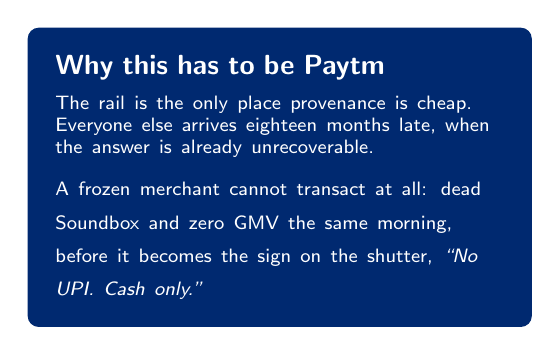
\begin{tikzpicture}\node[rounded corners=4pt,fill=navy,text=white,inner sep=10pt,text width=5.7cm,align=left]{
{\bfseries Why this has to be Paytm}\\[0.45em]
\scriptsize The rail is the only place provenance is cheap. Everyone else arrives eighteen months late, when the answer is already unrecoverable.\\[0.45em]
\scriptsize A frozen merchant cannot transact at all: dead Soundbox and zero GMV the same morning, before it becomes the sign on the shutter, \emph{\qm{No UPI. Cash only.}}
};\end{tikzpicture}
\end{column}
\end{columns}
\vspace{0.4cm}
\begin{center}
{\large\color{navy}\bfseries Paytm Hisaab}\quad{\color{muted}every rupee, on your side.}
\end{center}
\note{{\color{navy}\bfseries\normalsize 15.~The line we do not cross}\par\vspace{0.55em}\textbf{0:30 --- the non-negotiables, fast, then land.}
\\[0.4em]
Run the five bullets at pace. The one to hit is the first: we never assert
innocence on a freeze. The last is the mid-review answer, on the slide on purpose.
\\[0.4em]
Then the navy box: provenance is cheap only on the rail, and a frozen merchant
stops transacting the same morning.
\\[0.4em]
Final line, unhurried: \emph{``Paytm Hisaab. Every rupee, on your side.''} Stop talking.
\\[0.5em]
{\scriptsize
{\color{navy}\bfseries --- Q\&A prep ---}
\\[0.3em]
\textbf{``Merchants may not take personal money on a business QR.''} Correct, and
slide 11 says so before you have to. It arrives anyway, and the alternative to
recording it is letting an authority read it as income. We are not defending the
behaviour --- we are refusing to let it become a liability.
\\[0.3em]
\textbf{``Paytm already tags transactions.''} It does, and we build on that rather
than around it: channel, linked VPAs and payer history feed the rules layer. What
no tag carries is her attestation --- the part an authority accepts, and the only
part she alone can give.
\\[0.3em]
\textbf{``No return mismatch?''} That check needs a \emph{registered} composition
dealer who filed a CMP-08 to disagree with. Ours is unregistered, which is why she
gets a notice at all; the eval split has one with four quarters seeded.
\\[0.3em]
\textbf{``Exempt vs taxable on a QR sale?''} Not per payment. We apportion by value
from that shop's own POS-billed ratio and label it an estimate. Labelling each sale
by its majority side understated taxable turnover threefold.
\\[0.3em]
\textbf{``Four LLM calls in a trenchcoat?''} Everything deterministic is a skill and
four agents is the ceiling. If twenty lines of Python replaces an agent, it should
have been a skill --- the trace shows which is which.
\\[0.3em]
\textbf{``No standing with the police.''} Agreed: Paytm supplies, the merchant
files. By design. Cash sales are real, out of scope, and on the slide.}}
\end{frame}

\end{document}
"
\ifdefined\shownotes
  \setbeamertemplate{note page}{%
    \usebeamercolor[fg]{normal text}%
    \vspace{0.2em}%
    {\scriptsize\color{muted}Paytm Hisaab \;$\cdot$\; speaker notes}\hfill
    {\scriptsize\color{muted}slide \insertframenumber\ of 15}\par
    \vspace{0.25em}{\color{ptmcyan}\rule{\textwidth}{1.5pt}}\par
    \vspace{0.55em}\footnotesize\raggedright\insertnote\par}
  \setbeameroption{show only notes}
\fi

\begin{document}

% ============================================================ 1. TITLE
{\setbeamertemplate{footline}{}
\begin{frame}[plain]
\vspace{0.9cm}
\begin{center}
{\fontsize{38}{42}\selectfont\bfseries\color{navy}Paytm\;\color{ink}Hisaab}\\[0.45em]
{\Large\color{muted}Every rupee, on your side.}\\[0.9em]
{\color{ptmcyan}\rule{2.8cm}{2.5pt}}\\[0.9em]
{\large\color{ink}The agent that lets a merchant account for their own money}\\[0.15em]
{\large\color{ink}when someone in authority demands an explanation.}\\[1.3em]
{\small\color{muted}Agent Labs Buildathon \;$\cdot$\; Phinite $\times$ Paytm \;$\cdot$\; Track 2: AI for Small Businesses}
\end{center}
\note{{\color{navy}\bfseries\normalsize 1.~Title}\par\vspace{0.55em}\textbf{0:10 --- open cold.} Do not read the title or the tagline off the slide.
\\[0.4em]
Say: \emph{``I want to tell you about a man in Haveri who opened an envelope.''} Then advance.
\\[0.4em]
Nothing on this slide needs explaining. The tagline lands at the end, not here.}
\end{frame}}

% ============================================================ 2. STORY
\begin{frame}{Haveri, 2025}{A vegetable vendor opens an envelope}
\vspace{0.05cm}
\begin{columns}[T]
\begin{column}{0.52\textwidth}
\vspace{0.15cm}
He sells vegetables. Vegetables are \hi{exempt} from GST.\\[0.6em]
He also took UPI, because Paytm asked him to.\\[0.6em]
Four years of credits into his account, added up and billed as income:
\begin{center}\vspace{0.1em}{\fontsize{30}{32}\selectfont\bfseries\color{bad}₹29 lakh}\end{center}
\end{column}
\begin{column}{0.44\textwidth}
\ocard{hairline}{5.4cm}{\centering
  {\color{muted}\scriptsize Within weeks, on shutters across Karnataka:}\\[0.6em]
  {\fontsize{20}{23}\selectfont\bfseries\color{ink}\qm{No UPI.\\ Cash only.}}\\[0.6em]
  {\color{muted}\scriptsize A statewide boycott, by the merchants who had just adopted it.}}
\end{column}
\end{columns}
\vspace{0.25cm}
\hspace{0.1cm}{\small\sub{Withdrawn for the traders who could \emph{show} what they sold. Most could not. And tax is no longer the only authority asking.}}
\note{{\color{navy}\bfseries\normalsize 2.~Haveri, 2025}\par\vspace{0.55em}\textbf{0:45 --- the hook. Tell it, do not summarise it.}
\\[0.4em]
Four beats, in this order: he sells vegetables; vegetables are exempt from GST;
he took UPI because \emph{we} asked him to; the department added up four years of
credits and sent him a bill for \textbf{₹29 lakh}.
\\[0.4em]
\textbf{Pause on the number.} Then the card: within weeks, shutters across Karnataka
read ``No UPI, cash only.'' Merchants we had just onboarded, boycotting the rail.
\\[0.4em]
Close on the bottom line --- the notices were withdrawn for traders who could
\emph{show} what they sold. Most could not. That verb is the whole product.
\\[0.4em]
\textbf{Then the bridge:} \emph{``and tax is no longer the only authority asking.''}
That sentence is doing the repositioning --- Haveri is not a tax story here, it is
the moment taking digital money became a liability. The sharper version of it is
two slides away.
\\[0.4em]
\textbf{Do not say this is happening right now.} It is 2025. The next slide is
what makes it current, and a judge who knows the episode will respect the distinction.}
\end{frame}

% ============================================================ 3. STILL HAPPENING
\begin{frame}{And this is not a 2025 story}{CAclubindia, last updated 02 September 2026: ten days ago}
\vspace{0.1cm}
\begin{center}

\includegraphics[width=12.4cm]{gst-notices-2026.png}
\end{center}
\vspace{0.35cm}
\card{13.1cm}{\scriptsize\qm{During August 2026, the GST Department issued a significant number of notices covering different financial years and involving a wide range of issues\ldots\ They covered matters such as ITC mismatches, ineligible credit, \hi{differences in turnover}, wrong GST classification or rate, \hi{exemption claims}, Reverse Charge Mechanism\ldots}}
\vspace{0.3cm}

\hspace{0.1cm}{\small Those two categories are the whole content of an evidence pack. And this is the \emph{slower} of the two authorities. The other one freezes the account first.}
\note{{\color{navy}\bfseries\normalsize 3.~And this is not a 2025 story}\par\vspace{0.55em}\textbf{0:25 --- fast. This slide exists to kill one objection.}
\\[0.4em]
Say: \emph{``That was last year. This was published ten days ago.''}
\\[0.4em]
Do not read the quote. Point at the two bolded phrases only ---
\textbf{differences in turnover} and \textbf{exemption claims} --- and say those
two categories are the entire content of what we build.
\\[0.4em]
\textbf{Land on the last line and move.} It is the handoff into the police
slide: this is the slower authority. The other one freezes first and asks
afterwards. Do not linger here --- tax is no longer the headline.}
\end{frame}

% ============================================================ 4. THE TRAP
\begin{frame}{Every rupee a merchant receives is now evidence}{Today it is only ever used against them}
\vspace{0.05cm}
\begin{columns}[T]
\begin{column}{0.47\textwidth}
\ocard{bad}{6.0cm}{{\bfseries\color{bad}The cyber-crime police}\\[0.35em]
\scriptsize Fraud money layers through accounts within minutes. The shop at the end of the chain, the one that sold someone a watermelon, is frozen. It did nothing wrong, is not named in the FIR, and finds out when a payment declines.}
\end{column}
\begin{column}{0.47\textwidth}
\card{6.1cm}{{\bfseries\color{navy}The tax department}\\[0.35em]
\scriptsize Compares UPI collections against filed returns and bills the difference. Registered traders too, with QR, wallet, card and cash deposits all in scope.}
\end{column}
\end{columns}
\vspace{0.4cm}
\begin{center}
{\large Both demand the same artefact: \hi{what was each rupee, actually?}}\\[0.3em]
{\small\color{muted}Paytm already sees more of this than anyone. What is missing is the \emph{merchant's own answer}, captured when it is still knowable.}
\end{center}
\vspace{0.15cm}
{\color{hairline}\hrule height 1pt}
\vspace{0.35em}
\hspace{0.05cm}{\scriptsize\bfseries\color{bad}What it costs Paytm:}~{\scriptsize a frozen merchant stops transacting that morning. A frightened one takes the QR down for good. Dead Soundbox, zero GMV, no lending origination.}
\note{{\color{navy}\bfseries\normalsize 4.~Every rupee is now evidence}\par\vspace{0.55em}\textbf{0:40 --- two authorities, one unanswerable question.}
\\[0.4em]
\textbf{Left card first and give it the time.} Fraud money layers within minutes,
and the shop at the end of the chain, \emph{the one that sold someone a watermelon},
gets frozen. It did nothing wrong, it is not named in the FIR, and it finds out
when a payment declines. Use the watermelon.
\\[0.4em]
Right card briskly: the department reconciles collections against filed returns
and bills the difference. One sentence, then move.
\\[0.4em]
Then the pivot: both demand the same artefact --- what was each rupee, actually.
\\[0.4em]
\textbf{Say the grey line as written.} We do \emph{not} claim Paytm does nothing
with this data --- it tags plenty. The gap is the merchant's own answer, captured
when it is still knowable. Claiming otherwise in this room gets corrected.
\\[0.4em]
\textbf{Slow down for the red line.} This is the business case, not a footnote:
a frozen merchant stops transacting that morning, a frightened one takes the QR
down for good. Dead Soundbox, zero GMV, no lending origination.}
\end{frame}

% ============================================================ 5. THE BAR
\begin{frame}{Gross credits are not turnover}{One shop, one year, ₹60.98 lakh of credits}
\vspace{0.1cm}
\begin{center}
\begin{tikzpicture}[x=1cm,y=1cm]
% --- what the notice counts
\node[anchor=west,font=\scriptsize\bfseries,text=bad] at (-0.05,1.80) {WHAT THE NOTICE COUNTS AS TURNOVER};
\fill[bad!85,rounded corners=2pt] (0,1.06) rectangle (11.4,1.60);
\node[font=\small\bfseries,text=white] at (5.7,1.33) {₹60.98 lakh};

% --- what actually happened   (1 lakh = 0.18696 cm, so the bars are the same length)
\node[anchor=west,font=\scriptsize\bfseries,text=navy] at (-0.05,0.66) {WHAT ACTUALLY HAPPENED};
\fill[good!80,rounded corners=2pt]  (0,-0.08)     rectangle (6.001,0.46);
\fill[good!45]                      (6.001,-0.08) rectangle (8.002,0.46);
\fill[ptmcyan!70]                   (8.002,-0.08) rectangle (9.385,0.46);
\fill[navy!55]                      (9.385,-0.08) rectangle (10.451,0.46);
\fill[amber!70]                     (10.451,-0.08)rectangle (11.255,0.46);
\fill[muted!60,rounded corners=2pt] (11.255,-0.08)rectangle (11.4,0.46);

% brackets
\draw[navy,line width=0.8pt] (0,-0.22) -- (0,-0.36) -- (8.002,-0.36) -- (8.002,-0.22);
\node[anchor=north,font=\scriptsize,text=navy,align=center] at (4.0,-0.38)
  {\bfseries ₹42.9L aggregate turnover\quad{\color{muted}\scriptsize exempt ₹32.1L + taxable ₹10.7L}};
\draw[bad,line width=0.8pt] (8.002,-0.22) -- (8.002,-0.36) -- (11.4,-0.36) -- (11.4,-0.22);
\node[anchor=north,font=\scriptsize,text=bad,align=center] at (9.7,-0.38)
  {\bfseries ₹18.1L that is not turnover at all};

% legend
\node[font=\scriptsize,text=ink] at (5.7,-1.02) {%
\textcolor{good!80}{$\blacksquare$}~Exempt sales \quad
\textcolor{good!45}{$\blacksquare$}~Taxable sales \quad
\textcolor{ptmcyan!70}{$\blacksquare$}~Her own accounts ₹7.4L};
\node[font=\scriptsize,text=ink] at (5.7,-1.40) {%
\textcolor{navy!55}{$\blacksquare$}~Family ₹5.7L \quad
\textcolor{amber!70}{$\blacksquare$}~Loans, chit, gifts ₹4.3L \quad
\textcolor{muted!60}{$\blacksquare$}~Refunds \& duplicates ₹0.7L};
\end{tikzpicture}
\end{center}
\vspace{0.15cm}
\hspace{0.1cm}{\small\sub{Personal money does not belong on a business QR. It arrives anyway, reads as turnover, and hides the one credit the police will ask about.}}
\note{{\color{navy}\bfseries\normalsize 5.~Gross credits are not turnover}\par\vspace{0.55em}\textbf{0:45 --- the hinge of the pitch. Let the picture work.}
\\[0.4em]
Say: \emph{``One shop, one year, ₹60.98 lakh of credits. The red bar is what the
notice counts as turnover --- all of it.''}
\\[0.4em]
Then the bottom bar. \textbf{Stop talking for two seconds} and let them read it.
\\[0.4em]
₹42.9L really is turnover, and we say so. ₹18.1L is not: her savings account, her
husband, a chit payout, a double-tap on the Soundbox.
\\[0.4em]
\textbf{Get in front of the obvious objection.} Personal money is not supposed to
touch a business QR. Say so first, then say it arrives anyway --- that is an
observation about merchants, not a loophole we are selling. The rule does not stop
it; it only means no one is keeping a record of it.
\\[0.4em]
\textbf{And close on the second use.} This volume is also why she cannot find the
one credit the police care about. Same bar, same problem, and the freeze slide
pays it off.
\\[0.4em]
If challenged on the numbers: seeded ground truth from our generator, not an
estimate. Accuracy against it is slide 14.}
\end{frame}

% ============================================================ 6. INSIGHT
\begin{frame}{The insight}{Most teams would build the tax tool \emph{or} the fraud tool. They are the same engine.}
\vspace{0.15cm}
\begin{center}
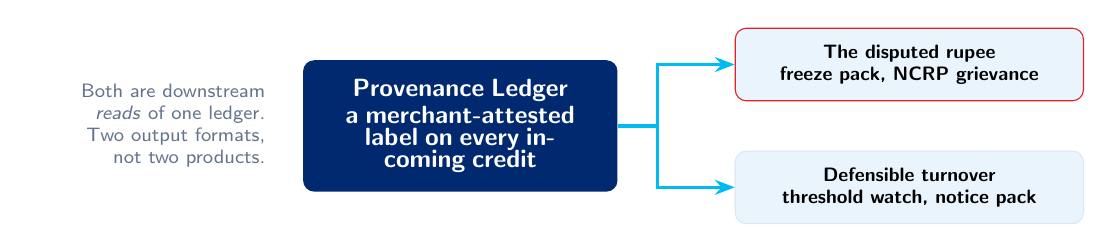
\begin{tikzpicture}[font=\scriptsize]
\node[rounded corners=4pt,fill=navy,text=white,inner sep=7pt,align=center,text width=3.5cm]
  (eng) {\bfseries\small Provenance Ledger\\[0.15em] a merchant-attested label on every incoming credit};
\node[rounded corners=4pt,fill=tint,draw=bad,inner sep=6pt,align=center,text width=4.0cm]
  (tax) at ($(eng.east)+(3.7,0.78)$) {\bfseries The disputed rupee\\ freeze pack, NCRP grievance};
\node[rounded corners=4pt,fill=tint,draw=hairline,inner sep=6pt,align=center,text width=4.0cm]
  (fra) at ($(eng.east)+(3.7,-0.78)$) {\bfseries Defensible turnover\\ threshold watch, notice pack};
\draw[-{Stealth[length=2.5mm]},ptmcyan,line width=1.3pt] (eng.east) -- ++(0.5,0) |- (tax.west);
\draw[-{Stealth[length=2.5mm]},ptmcyan,line width=1.3pt] (eng.east) -- ++(0.5,0) |- (fra.west);
\node[anchor=east,text width=2.9cm,align=right,text=muted] at ($(eng.west)+(-0.35,0)$)
  {Both are downstream \emph{reads} of one ledger. Two output formats, not two products.};
\end{tikzpicture}
\end{center}
\vspace{0.1cm}
\begin{center}
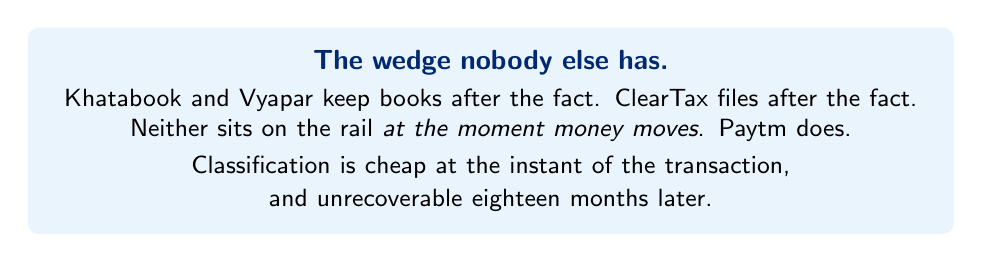
\begin{tikzpicture}\node[rounded corners=4pt,fill=tint,inner sep=8pt,text width=11.2cm,align=center]{
{\bfseries\color{navy}The wedge nobody else has.}\\[0.25em]
\small Khatabook and Vyapar keep books after the fact. ClearTax files after the fact.\\
Neither sits on the rail \emph{at the moment money moves}. Paytm does.\\[0.25em]
\small Classification is cheap at the instant of the transaction,\\ and unrecoverable eighteen months later.
};\end{tikzpicture}
\end{center}
\note{{\color{navy}\bfseries\normalsize 6.~The insight}\par\vspace{0.55em}\textbf{0:40 --- why this is one product, not two.}
\\[0.4em]
Say: \emph{``Most teams would build the fraud tool or the tax tool. They are the
same engine.''} Both are downstream reads of one ledger --- two output formats,
and the freeze pack is the one we lead with.
\\[0.4em]
Then the wedge, and say it slowly because it is the defensible-moat answer:
Khatabook and Vyapar keep books after the fact, ClearTax files after the fact.
Neither sits on the rail at the moment money moves. \textbf{Paytm does.}
\\[0.4em]
Landing line: classification is cheap and accurate at the instant of the
transaction, and unrecoverable eighteen months later when the notice arrives.}
\end{frame}

% ============================================================ 7. THE ENGINE
\begin{frame}{The engine}{Eight tags, one tap}
\vspace{0.15cm}
\begin{columns}[T]
\begin{column}{0.45\textwidth}
{\color{navy}\bfseries\small Every incoming credit gets one tag}\\[0.4em]
{\scriptsize
\begin{tabular}{@{}ll@{}}
\texttt{taxable\_supply}    & ordinary sale \\
\texttt{exempt\_supply}     & vegetables, milk, loose rice \\
\texttt{personal\_transfer} & spouse, parent, sibling \\
\texttt{inter\_account}     & her own money \\
\texttt{refund\_reversal}   & money back from a vendor \\
\texttt{duplicate}          & paid twice, one refunded \\
\texttt{non\_business}      & loan, chit payout, gift \\
{\color{bad}\texttt{unclassified}} & {\color{bad}not enough signal: ask her} \\
\end{tabular}}
\\[0.75em]
{\scriptsize\color{muted}98.6\% are ordinary sales, settled by rules. The agent reasons only about the 1.4\% that need judgement.}
\end{column}
\begin{column}{0.51\textwidth}
\card{6.6cm}{{\bfseries\color{navy}The agent proposes. The merchant attests.}\\[0.4em]
\scriptsize You cannot infer \qm{my husband sent this} from a QR payment. The agent proposes a tag \emph{with its reason}; she confirms with one tap, in Kannada, batched daily.\\[0.45em]
\scriptsize Not a fallback. A ledger she attested \emph{at the time} survives a hearing. An algorithm's guess, made under duress a year later, does not.}
\\[0.55em]
\hspace{0.15cm}\begin{minipage}{6.6cm}
{\bfseries\color{navy}\small Budget: at most 3 questions a day.}\\[0.15em]
{\scriptsize\color{muted}Over a simulated year: \hi{189 questions, median 1.3 a day}. Ask more and the product is dead.}
\end{minipage}
\end{column}
\end{columns}
\note{{\color{navy}\bfseries\normalsize 7.~The engine}\par\vspace{0.55em}\textbf{0:45 --- the mechanism. Do not read the tag list.}
\\[0.4em]
Gesture at the eight tags, say ``eight labels, every incoming credit gets one,''
and move to the right-hand card, which is the real content.
\\[0.4em]
\textbf{The line that matters:} you cannot infer ``my husband sent this'' from a
QR payment. So the agent proposes a tag \emph{with its reason} and she confirms
with one tap. This is not a fallback --- a ledger she attested contemporaneously
survives a hearing; an algorithm's guess produced under duress a year later does not.
\\[0.4em]
Then the budget: at most three questions a day, and we measured 189 across a
year, median 1.3. Ask more than that and the product is dead.
\\[0.4em]
If asked about cost: 98.6\% are ordinary sales settled by rules. The model only
sees the 1.4\% that need judgement.}
\end{frame}

% ============================================================ 8. PRODUCT
\begin{frame}{What the merchant sees}
\vspace{-0.1cm}
\begin{center}
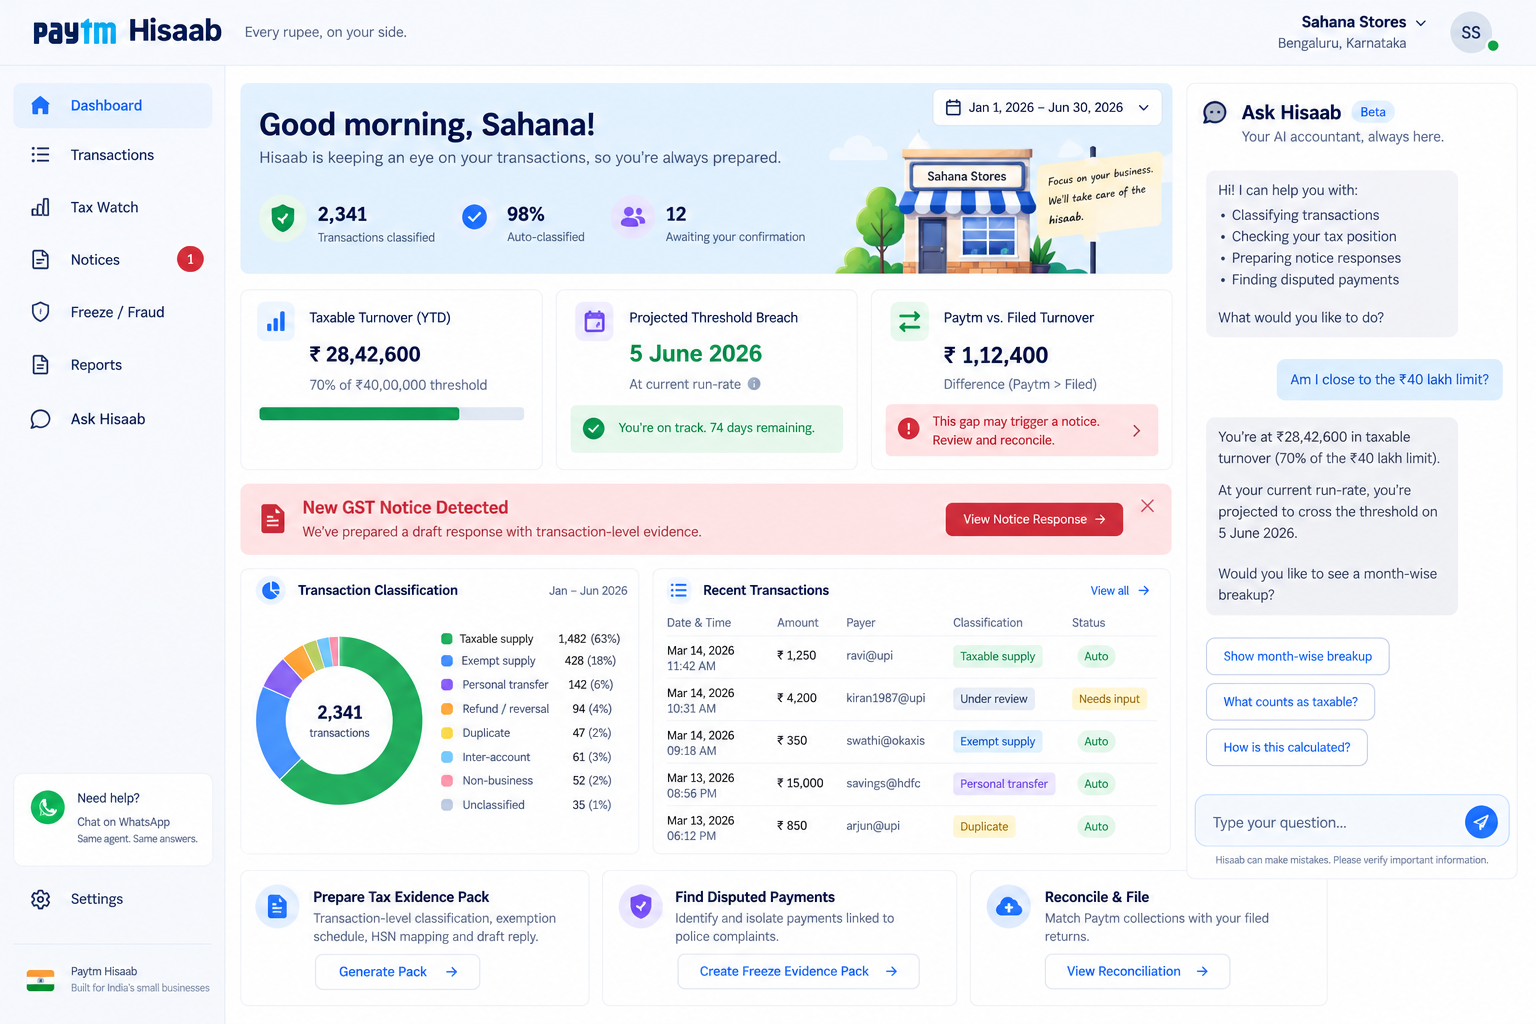
\includegraphics[width=\textwidth,height=0.70\textheight,keepaspectratio]{Paytm-Hisaab_website_look.png}
\end{center}
\vspace{0.1cm}
\hspace{0.05cm}{\scriptsize\color{muted}One surface: what every payment was classified as, how close she is to the threshold, and the packs. The same agent runs on WhatsApp, where she actually is.}
\note{{\color{navy}\bfseries\normalsize 8.~What the merchant sees}\par\vspace{0.55em}\textbf{0:20 --- a glance slide. Do not tour the UI.}
\\[0.4em]
One sentence: everything classified, how close she is to the threshold, and the
packs, on one surface.
\\[0.4em]
Then the WhatsApp point --- the same agent, where she actually is --- and advance.
\\[0.4em]
If someone asks whether this is built: the chat and the tools are live; this
screen is the product surface we are designing toward.}
\end{frame}

% ============================================================ 9. ARCHITECTURE
\begin{frame}{Built on Phinite}{Two agent graphs, four agents, ten deterministic skills}
\vspace{0.15cm}
\begin{columns}[T]
\begin{column}{0.53\textwidth}
{\scriptsize
\begin{tabular}{@{}L{1.75cm}L{4.7cm}@{}}
\multicolumn{2}{@{}l}{\color{navy}\bfseries\small hisaab-watch \;\scriptsize(autonomous: cron + API)}\\
\midrule
Provenance & proposes a tag and a reason for the hard credits \\
Evidence   & assembles packs: freeze evidence, then exemption schedules and HSN \\
\addlinespace[0.6em]
\multicolumn{2}{@{}l}{\color{navy}\bfseries\small hisaab-merchant \;\scriptsize(conversational: chat)}\\
\midrule
Merchant   & the conversation: attestation, alerts, Kannada \\
Escalation & decides when to stop and route to a human CA \\
\bottomrule
\end{tabular}}
\\[0.75em]
{\scriptsize\color{muted}The nightly pass writes its queue to the ledger; the chat reads it when she opens it. Deliberately \emph{not} a graph-to-graph call: a queue that outlives either run is what makes the handoff robust.}
\end{column}
\begin{column}{0.44\textwidth}
\card{5.7cm}{{\bfseries\color{navy}Permissions are the product}\\[0.4em]
\scriptsize Provenance proposes, \red{never commits}.\\[0.25em]
\scriptsize Merchant is the \emph{only} agent that can commit a tag.\\[0.25em]
\scriptsize Evidence is \red{read-only}. It cannot edit a classification to make a pack look better.\\[0.25em]
\scriptsize Escalation can \red{halt} any pack; a human approves.}
\\[0.5em]
\hspace{0.1cm}\begin{minipage}{5.7cm}{\scriptsize\color{muted}Ten tools run live against a hosted service. Every number in a pack traces back, in the trace, to the credit and the attestation behind it.}\end{minipage}
\end{column}
\end{columns}
\note{{\color{navy}\bfseries\normalsize 9.~Built on Phinite}\par\vspace{0.55em}\textbf{0:40 --- for the technical judges.}
\\[0.4em]
Two agent graphs, not four loose agents: \texttt{hisaab-watch} runs autonomously on
cron, \texttt{hisaab-merchant} is the conversation. The nightly pass writes a queue;
the chat reads it when she opens it --- deliberately not a graph-to-graph call,
because a queue that outlives either run is what makes the handoff robust.
\\[0.4em]
\textbf{Spend your time on the right-hand card.} The strongest line in it:
the Evidence agent is read-only --- \emph{the agent that builds the defence cannot
edit the evidence.} And only the Merchant agent can commit an attested tag.
\\[0.4em]
Those are enforced as Phinite tool policies, not conventions, and a denied call
shows up in the trace.}
\end{frame}

% ============================================================ 10. DESIGN DECISIONS
\begin{frame}{Four decisions that make it defensible}
\vspace{0.3cm}
\begin{columns}[T]
\begin{column}{0.48\textwidth}
\card{6.0cm}{{\bfseries\color{navy}1. Arithmetic lives in skills, not the model}\\[0.35em]
\scriptsize Turnover, projections and apportionment are deterministic Python: versioned, testable, traceable. Wrapping arithmetic in an LLM is the standard tell, and the trace would show it.}
\\[0.35em]
\card{6.0cm}{{\bfseries\color{navy}3. Refusing to guess is a feature}\\[0.35em]
\scriptsize An \texttt{unclassified} credit routed to the merchant costs one tap. A confident wrong tag inside an evidence pack is a catastrophe. We report the refusal rate honestly.}
\end{column}
\begin{column}{0.48\textwidth}
\card{6.0cm}{{\bfseries\color{navy}2. Attestation is the promotion boundary}\\[0.35em]
\scriptsize Nothing enters a production pack that the merchant has not confirmed. Sandbox to UAT to prod, with her tap as the gate.}
\\[0.35em]
\card{6.0cm}{{\bfseries\color{navy}4. Ground truth, so accuracy is a number}\\[0.35em]
\scriptsize We simulated a year of a shop's life from a known process, split into what Paytm can see and what really happened. Agents read only the visible half, which is why we quote error bars instead of vibes.}
\end{column}
\end{columns}
\note{{\color{navy}\bfseries\normalsize 10.~Four decisions}\par\vspace{0.55em}\textbf{0:35 --- the slide that separates you from a demo.}
\\[0.4em]
Lead with \#1: all arithmetic is deterministic Python, not model output. Wrapping
arithmetic in an LLM is the standard tell, and the trace would show it.
\\[0.4em]
Then \#3: refusing to guess is a feature. An \texttt{unclassified} credit costs one
tap; a confident wrong tag inside an evidence pack is a catastrophe.
\\[0.4em]
Skim \#2 and \#4 --- one clause each. \#4 is worth a beat if the room is technical:
we generated ground truth, so accuracy is a number instead of a claim.}
\end{frame}

% ============================================================ 11. DEMO / ATTESTATION
\begin{frame}{Demo $\cdot$ Sahana Stores, Jayanagar}{An ordinary Tuesday, before anything goes wrong}
\vspace{0.1cm}
\begin{columns}[T]
\begin{column}{0.48\textwidth}
{\scriptsize\color{muted}Tuesday 10 March. Thirty-nine credits came in over the weekend. The agent asks about \hi{three}.}
\\[0.4em]
\card{5.9cm}{{\kn\scriptsize ಭಾನುವಾರ ರಾತ್ರಿ ₹15,000. ನಿಮ್ಮ ಸ್ವಂತ ಹಣವೇ?}\\[0.25em]
{\color{muted}\scriptsize \qm{₹15,000 at 11:04pm Sunday, from your savings account. Your own money?}}\\[0.35em]
{\scriptsize\color{navy}\fbox{\kn ಹೌದು}\;\fbox{\kn ಇಲ್ಲ}}}
\\[0.4em]
{\scriptsize $\cdot$\; ₹7,500 from her husband, scanned at the shop QR\\[0.25em]
$\cdot$\; ₹4,850 from Raghu Shetty, who has bought twice before. A real sale, and the agent \emph{asks} rather than assumes.}
\\[0.4em]
{\scriptsize\color{muted}The other thirty-six settle silently, and a ₹23 payment nobody can place is left alone.}
\end{column}
\begin{column}{0.48\textwidth}
\ocard{amber}{6.1cm}{{\bfseries\color{amber}And yes, two of those three should not be there}\\[0.35em]
\scriptsize A business QR is not for personal money, and the terms say so. It arrives anyway: family, own top-ups, a chit payout. The rule does not prevent it. It only means \emph{nobody keeps a record of it.}}
\\[0.45em]
{\scriptsize Paytm already reads the signals: channel, linked VPAs, payer history. What no system has is the \hi{merchant's own answer}, given at the time, in her language, and kept.}
\\[0.45em]
{\scriptsize That record is what the next two slides are built from: first for the police, then for the department.}
\end{column}
\end{columns}
\note{{\color{navy}\bfseries\normalsize 11.~Demo --- an ordinary Tuesday (beat 1)}\par\vspace{0.55em}\textbf{0:45 --- or hand over to the live demo here.}
\\[0.4em]
Thirty-nine credits came in over the weekend, the agent asks about \textbf{three}.
Read the Kannada line if you can; otherwise read the gloss under it.
\\[0.4em]
\textbf{Do not hide from the right-hand card --- lead with it.} The mid-review
point was that personal money is not allowed on a business QR. Correct, and we say
so on the slide. The argument is that the rule does not stop it, it only means no
one records it, and an unrecorded credit is what an authority later reads as income.
\\[0.4em]
\textbf{Second half of that card matters just as much.} We are not claiming Paytm
does nothing. It already reads channel, linked VPAs and payer history. What no
system has is her own answer, captured while it is still knowable. That is the
product, and it is a smaller, truer claim than the one we started with.
\\[0.4em]
\textbf{Before going on stage:} confirm the attestation queue is whole ---
\texttt{pending\_total} must be 3. A rehearsal that taps through this beat spends the
queue, and Render needs a clear-cache redeploy to restore it.}
\end{frame}

% ============================================================ 12. DEMO / THE FREEZE
\begin{frame}{Demo $\cdot$ The emergency}{The account is frozen at 09:30 and the supplier payment is due}
\vspace{0.2cm}
\begin{columns}[T]
\begin{column}{0.46\textwidth}
{\scriptsize She sold someone 12kg of onions. That customer was three layers downstream of a fraud victim. She is not named in the FIR, which was filed in another state, and \hi{339 payments} came in that week.}
\\[0.5em]
\card{5.8cm}{{\bfseries\color{navy}The agent isolates it}\\[0.35em]
\scriptsize ₹4,200 on 21 March at 19:47, till POS01. Matched by UTR \emph{and independently} by amount and date.\\[0.3em]
\scriptsize The sale record comes with it: the POS bill, the items, the till and the minute.}
\end{column}
\begin{column}{0.49\textwidth}
\ocard{amber}{6.1cm}{{\bfseries\color{amber}And the decoy it did not choose}\\[0.35em]
\scriptsize A \emph{second} ₹4,200 that same week, from a regular customer. Listed in the pack, and explicitly \emph{not} named as the disputed one. Only the date separates them.}
\\[0.5em]
{\scriptsize Then it drafts the NCRP-CFCFRMS grievance, citing the judgments that only the \emph{disputed amount} should be lien-marked, not the whole account.}
\\[0.5em]
{\scriptsize\color{bad}\bfseries It never asserts that she is innocent.}\\[0.1em]
{\scriptsize\color{muted}Some frozen accounts genuinely are mule accounts. The agent assembles evidence; a human decides. Escalation holds the pack for approval.}
\end{column}
\end{columns}
\note{{\color{navy}\bfseries\normalsize 12.~Demo --- the emergency (beat 4)}\par\vspace{0.55em}\textbf{0:50 --- this is now the lead case. Give it the most time of the three.}
\\[0.4em]
Set the stakes in one sentence: account frozen at half nine, supplier payment due,
339 payments came in that week, and she is not named in the FIR.
\\[0.4em]
\textbf{Why this one leads.} She did nothing wrong and there is no rule she broke.
She sold onions to a customer who turned out to be laundering. Every objection
available against the tax case --- she should not have taken personal money on that
QR, she should have registered --- has no purchase here at all.
\\[0.4em]
The agent isolates ₹4,200 by UTR \emph{and independently} by amount and date, and
brings the POS bill with it --- the items, till POS01, 19:47.
\\[0.4em]
\textbf{The decoy is the point.} A second ₹4,200 that same week from a regular
customer, listed in the pack and explicitly not chosen. Anyone can match an amount;
the pack shows its work.
\\[0.4em]
Finish on the red line: it never asserts she is innocent. Some frozen accounts
genuinely are mule accounts. We assemble evidence; a human decides, and Escalation
holds the pack for approval.}
\end{frame}

% ============================================================ 13. DEMO / TAX
\begin{frame}{Demo $\cdot$ The warning, and the notice}{The same ledger, read for the other authority}
\vspace{0.15cm}
\begin{columns}[T]
\begin{column}{0.38\textwidth}
{\scriptsize\color{muted}Replayed as of 31 January:}
\\[0.35em]
\ocard{good}{4.8cm}{{\bfseries\color{ink}\scriptsize\qm{At your current rate you cross ₹40 lakh around {\color{bad}14 March}. You will need to register.}}\\[0.35em]
{\scriptsize\color{muted}\grn{43 days of warning}, and the date is computed, not typed.}}
\\[0.45em]
{\scriptsize\color{bad}\bfseries This beat is what makes the pitch safe.}\\[0.1em]
{\scriptsize\color{muted}Its first act on the tax side is telling her to register.}
\end{column}
\begin{column}{0.58\textwidth}
{\scriptsize\color{muted}Then the notice arrives, claiming {\color{bad}\bfseries ₹60.98L} of turnover:}
\\[0.3em]
{\scriptsize
\begin{tabular}{@{}lr@{\hskip 1.2em}l@{}}
\multicolumn{2}{@{}l}{\color{navy}\bfseries Aggregate turnover \quad ₹42.2L} & \sub{within \grn{1.6\%} of truth} \\
\midrule
Exempt supplies      & ₹31.3L & \sub{vegetables, loose rice} \\
Taxable supplies     & ₹10.9L & \sub{branded goods, oil, soap} \\
\addlinespace[0.45em]
\multicolumn{2}{@{}l}{\color{navy}\bfseries Not turnover at all \quad ₹18.8L} & \sub{every line traced} \\
\midrule
Her own accounts     & ₹7.4L & \sub{top-ups before supplier runs} \\
Family               & ₹6.1L & \sub{spouse, parent, in-law} \\
Loans, chit, gifts   & ₹4.3L & \sub{chit payout, festival gifts} \\
Refunds, duplicates  & ₹1.0L & \sub{crate returns, double-taps} \\
\bottomrule
\end{tabular}}
\\[0.45em]
{\scriptsize And it says plainly: \hi{the claim is wrong, and you \emph{did} cross ₹40 lakh on 14 March. You must register.}}
\end{column}
\end{columns}
\note{{\color{navy}\bfseries\normalsize 13.~Demo --- the warning and the notice (beats 2 and 3)}\par\vspace{0.55em}\textbf{0:50 --- two tax beats on one slide, deliberately compressed.}
\\[0.4em]
Left: replayed as of 31 January, the agent says she crosses ₹40 lakh around
14 March. \textbf{Say the red line out loud} --- its first act on the tax side is
telling her she owes a registration. That is what stops the room turning hostile.
\\[0.4em]
Right: the notice claims ₹60.98 lakh, and the pack answers it line by line, every
figure traceable to transaction IDs. Then the honest half:
\textbf{the claim is wrong, and she did cross ₹40 lakh, and she must register.}
\\[0.4em]
\textbf{If a judge diffs this against slide 5:} slide 5 shows seeded truth
(₹42.9L), this shows what our system computed (₹42.2L). The 1.6\% between them
\emph{is} the accuracy claim --- say that, do not hedge.
\\[0.4em]
\textbf{If pushed on the personal and own-account lines:} same answer as slide 11.
Those credits should not be on a business QR, they are there anyway, and the
alternative to classifying them is letting them be read as income.}
\end{frame}

% ============================================================ 14. NUMBERS
\begin{frame}{What we can actually prove}{One merchant, one year, 13,267 credits, scored against seeded truth}
\vspace{0.45cm}
\begin{columns}[T]
\begin{column}{0.33\textwidth}
\begin{center}\bignum{1.6\%}{error on aggregate turnover\\ (taxable share within 1\%)}\end{center}
\vspace{0.55cm}
\begin{center}\bignum{43 days}{of warning before the\\ threshold crossing}\end{center}
\end{column}
\begin{column}{0.33\textwidth}
\begin{center}\bignum{1.3 a day}{median questions asked.\\ 189 in a year, never over 3}\end{center}
\vspace{0.55cm}
\begin{center}\bignum{zero}{credits left untagged\\ across the whole year}\end{center}
\end{column}
\begin{column}{0.30\textwidth}
\card{3.8cm}{{\bfseries\color{navy}The honest baseline}\\[0.35em]
\scriptsize A 50-line rules-only classifier gets 99.3\% on sale vs not-a-sale, but catches only \red{77.8\%} of non-sale credits.\\[0.3em]
\scriptsize That residue alone puts two eval merchants on the \emph{wrong side} of ₹40L.\\[0.3em]
\scriptsize Closing it is what the agent plus one tap is for.}
\end{column}
\end{columns}
\vspace{0.45cm}
\hspace{0.1cm}{\scriptsize\color{muted}She corrected the agent 52 times that year. Those corrections are the ledger's strongest evidence, not its failures.}
\note{{\color{navy}\bfseries\normalsize 14.~What we can actually prove}\par\vspace{0.55em}\textbf{0:30 --- do not read all four. Pick two.}
\\[0.4em]
Lead with \textbf{1.6\%} error on turnover and \textbf{1.3 questions a day}. The
other two are there to be read, not narrated.
\\[0.4em]
\textbf{The credibility move is the box on the right} --- volunteer the weakness
before anyone finds it. A rules-only baseline gets 99.3\% on sale vs not-a-sale
but catches only 77.8\% of non-sale credits, and that residue alone puts two eval
merchants on the wrong side of ₹40 lakh. Closing it is what the agent plus one tap is for.
\\[0.4em]
Last line if you have the beat: she corrected the agent 52 times that year, and
those corrections are the ledger's strongest evidence, not its failures.}
\end{frame}

% ============================================================ 15. CLOSE
\begin{frame}{The line we do not cross}{Accuracy, not minimisation}
\vspace{0.3cm}
\begin{columns}[T]
\begin{column}{0.52\textwidth}
{\scriptsize
$\cdot$\; We \hi{never assert innocence} on a freeze. Some accounts really are mule accounts. We assemble evidence; a human decides.\\[0.5em]
$\cdot$\; We \hi{file nothing} with any authority. Artefacts only; the merchant or their CA files.\\[0.5em]
$\cdot$\; We compute what she \hi{genuinely owes} and say so plainly, including \qm{you crossed the threshold, you must register.}\\[0.5em]
$\cdot$\; We \hi{never assert a final liability}. We compute, show the workings, and route to a CA.\\[0.5em]
$\cdot$\; A business QR is \hi{not for personal money}. We do not excuse it. We record it, so it is not read as income.}
\end{column}
\begin{column}{0.44\textwidth}
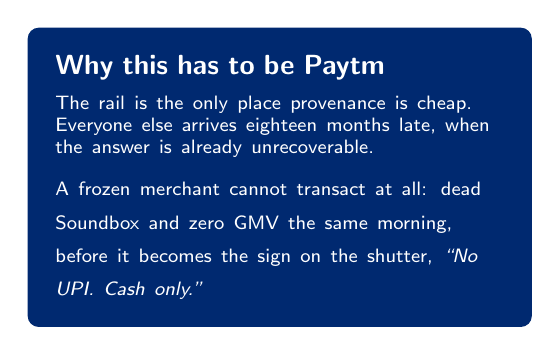
\begin{tikzpicture}\node[rounded corners=4pt,fill=navy,text=white,inner sep=10pt,text width=5.7cm,align=left]{
{\bfseries Why this has to be Paytm}\\[0.45em]
\scriptsize The rail is the only place provenance is cheap. Everyone else arrives eighteen months late, when the answer is already unrecoverable.\\[0.45em]
\scriptsize A frozen merchant cannot transact at all: dead Soundbox and zero GMV the same morning, before it becomes the sign on the shutter, \emph{\qm{No UPI. Cash only.}}
};\end{tikzpicture}
\end{column}
\end{columns}
\vspace{0.4cm}
\begin{center}
{\large\color{navy}\bfseries Paytm Hisaab}\quad{\color{muted}every rupee, on your side.}
\end{center}
\note{{\color{navy}\bfseries\normalsize 15.~The line we do not cross}\par\vspace{0.55em}\textbf{0:30 --- the non-negotiables, fast, then land.}
\\[0.4em]
Run the five bullets at pace. The one to hit is the first: we never assert
innocence on a freeze. The last is the mid-review answer, on the slide on purpose.
\\[0.4em]
Then the navy box: provenance is cheap only on the rail, and a frozen merchant
stops transacting the same morning.
\\[0.4em]
Final line, unhurried: \emph{``Paytm Hisaab. Every rupee, on your side.''} Stop talking.
\\[0.5em]
{\scriptsize
{\color{navy}\bfseries --- Q\&A prep ---}
\\[0.3em]
\textbf{``Merchants may not take personal money on a business QR.''} Correct, and
slide 11 says so before you have to. It arrives anyway, and the alternative to
recording it is letting an authority read it as income. We are not defending the
behaviour --- we are refusing to let it become a liability.
\\[0.3em]
\textbf{``Paytm already tags transactions.''} It does, and we build on that rather
than around it: channel, linked VPAs and payer history feed the rules layer. What
no tag carries is her attestation --- the part an authority accepts, and the only
part she alone can give.
\\[0.3em]
\textbf{``No return mismatch?''} That check needs a \emph{registered} composition
dealer who filed a CMP-08 to disagree with. Ours is unregistered, which is why she
gets a notice at all; the eval split has one with four quarters seeded.
\\[0.3em]
\textbf{``Exempt vs taxable on a QR sale?''} Not per payment. We apportion by value
from that shop's own POS-billed ratio and label it an estimate. Labelling each sale
by its majority side understated taxable turnover threefold.
\\[0.3em]
\textbf{``Four LLM calls in a trenchcoat?''} Everything deterministic is a skill and
four agents is the ceiling. If twenty lines of Python replaces an agent, it should
have been a skill --- the trace shows which is which.
\\[0.3em]
\textbf{``No standing with the police.''} Agreed: Paytm supplies, the merchant
files. By design. Cash sales are real, out of scope, and on the slide.}}
\end{frame}

\end{document}
"
%                                                     -> speaker notes, one page per slide
%
% Speaker notes live in the \note{} after each frame, so they cannot drift
% out of sync with the slides. Build both with: ./build.sh
%
% Fonts: Segoe UI + Nirmala UI (both ship with Windows). On another OS the
% deck still builds -- it falls back to the default sans and drops the
% Kannada styling.
\documentclass[aspectratio=169,10pt]{beamer}

\usepackage{fontspec}
\usepackage{tikz}
\usepackage{booktabs}
\usepackage{array}
\newcolumntype{L}[1]{>{\raggedright\arraybackslash}p{#1}}
\usepackage{graphicx}
\usetikzlibrary{calc,positioning,arrows.meta}

\graphicspath{{./}{../}}

% ---------- fonts ----------
\IfFontExistsTF{Segoe UI}{\setsansfont{Segoe UI}}{}
\IfFontExistsTF{Nirmala UI}{%
  \newfontfamily\kn[Script=Kannada]{Nirmala UI}}{%
  \newcommand{\kn}{}}
\renewcommand{\familydefault}{\sfdefault}

% ragged, unhyphenated text inside the narrow cards
\hyphenpenalty=10000
\exhyphenpenalty=10000
\emergencystretch=3em
\hbadness=10000

% ---------- palette (taken from the product mock) ----------
\definecolor{navy}{HTML}{002970}
\definecolor{ptmcyan}{HTML}{00BAF2}
\definecolor{ink}{HTML}{0F172A}
\definecolor{muted}{HTML}{64748B}
\definecolor{good}{HTML}{15803D}
\definecolor{bad}{HTML}{DC2626}
\definecolor{amber}{HTML}{B45309}
\definecolor{tint}{HTML}{EAF4FD}
\definecolor{hairline}{HTML}{DBE7F3}

% ---------- theme ----------
\usetheme{default}
\usecolortheme{default}
\setbeamertemplate{navigation symbols}{}
\setbeamersize{text margin left=0.85cm,text margin right=0.85cm}
\setbeamercolor{normal text}{fg=ink,bg=white}
\setbeamercolor{frametitle}{fg=navy}
\setbeamercolor{structure}{fg=navy}
\setbeamerfont{frametitle}{size=\large,series=\bfseries}
\setbeamerfont{framesubtitle}{size=\scriptsize}
\setbeamercolor{framesubtitle}{fg=muted}
\setbeamertemplate{frametitle}{%
  \vspace{0.30cm}%
  \usebeamerfont{frametitle}\usebeamercolor[fg]{frametitle}\insertframetitle%
  \ifx\insertframesubtitle\empty\else{\\[-0.15em]\usebeamerfont{framesubtitle}\usebeamercolor[fg]{framesubtitle}\insertframesubtitle}\fi%
  \\[0.1em]{\color{ptmcyan}\rule{1.2cm}{2pt}}\par\vspace{-0.15em}%
}
\setbeamertemplate{footline}{%
  \hbox{\begin{beamercolorbox}[wd=\paperwidth,ht=1.9ex,dp=1.1ex,leftskip=0.85cm,rightskip=0.85cm]{}%
  {\scriptsize\color{muted}Paytm Hisaab\hfill\insertframenumber}%
  \end{beamercolorbox}}%
}
\setbeamerfont{itemize/enumerate body}{size=\normalsize}

% ---------- helpers ----------
\newcommand{\hi}[1]{{\color{navy}\bfseries #1}}
\newcommand{\red}[1]{{\color{bad}\bfseries #1}}
\newcommand{\grn}[1]{{\color{good}\bfseries #1}}
\newcommand{\sub}[1]{{\color{muted}#1}}
\newcommand{\qm}[1]{``#1''}
\newcommand{\bignum}[2]{{\color{navy}\fontsize{22}{24}\selectfont\bfseries #1}\\[0.1em]{\scriptsize\color{muted}#2}}
% a soft rounded card:  \card{width}{body}
\newcommand{\card}[2]{\begin{tikzpicture}%
  \node[rounded corners=4pt,fill=tint,inner sep=8pt,text width=#1,align=left]{#2};%
  \end{tikzpicture}}
% an outlined card:  \ocard{colour}{width}{body}
\newcommand{\ocard}[3]{\begin{tikzpicture}%
  \node[rounded corners=4pt,fill=white,draw=#1,line width=0.9pt,inner sep=8pt,text width=#2,align=left]{#3};%
  \end{tikzpicture}}

% ---------- presenter build ----------
% Set after every colour and template above, so the composed notes page keeps
% the deck's own colours:
%   xelatex -jobname=hisaab-pitch-notes "\def\shownotes{1}% Paytm Hisaab -- buildathon pitch deck
%
% Compile with XeLaTeX (needed for the rupee sign and the Kannada line):
%
%   cd pitch
%   xelatex hisaab-pitch.tex                          -> hisaab-pitch.pdf  (slides)
%   xelatex -jobname=hisaab-pitch-notes "\def\shownotes{1}% Paytm Hisaab -- buildathon pitch deck
%
% Compile with XeLaTeX (needed for the rupee sign and the Kannada line):
%
%   cd pitch
%   xelatex hisaab-pitch.tex                          -> hisaab-pitch.pdf  (slides)
%   xelatex -jobname=hisaab-pitch-notes "\def\shownotes{1}% Paytm Hisaab -- buildathon pitch deck
%
% Compile with XeLaTeX (needed for the rupee sign and the Kannada line):
%
%   cd pitch
%   xelatex hisaab-pitch.tex                          -> hisaab-pitch.pdf  (slides)
%   xelatex -jobname=hisaab-pitch-notes "\def\shownotes{1}\input{hisaab-pitch.tex}"
%                                                     -> speaker notes, one page per slide
%
% Speaker notes live in the \note{} after each frame, so they cannot drift
% out of sync with the slides. Build both with: ./build.sh
%
% Fonts: Segoe UI + Nirmala UI (both ship with Windows). On another OS the
% deck still builds -- it falls back to the default sans and drops the
% Kannada styling.
\documentclass[aspectratio=169,10pt]{beamer}

\usepackage{fontspec}
\usepackage{tikz}
\usepackage{booktabs}
\usepackage{array}
\newcolumntype{L}[1]{>{\raggedright\arraybackslash}p{#1}}
\usepackage{graphicx}
\usetikzlibrary{calc,positioning,arrows.meta}

\graphicspath{{./}{../}}

% ---------- fonts ----------
\IfFontExistsTF{Segoe UI}{\setsansfont{Segoe UI}}{}
\IfFontExistsTF{Nirmala UI}{%
  \newfontfamily\kn[Script=Kannada]{Nirmala UI}}{%
  \newcommand{\kn}{}}
\renewcommand{\familydefault}{\sfdefault}

% ragged, unhyphenated text inside the narrow cards
\hyphenpenalty=10000
\exhyphenpenalty=10000
\emergencystretch=3em
\hbadness=10000

% ---------- palette (taken from the product mock) ----------
\definecolor{navy}{HTML}{002970}
\definecolor{ptmcyan}{HTML}{00BAF2}
\definecolor{ink}{HTML}{0F172A}
\definecolor{muted}{HTML}{64748B}
\definecolor{good}{HTML}{15803D}
\definecolor{bad}{HTML}{DC2626}
\definecolor{amber}{HTML}{B45309}
\definecolor{tint}{HTML}{EAF4FD}
\definecolor{hairline}{HTML}{DBE7F3}

% ---------- theme ----------
\usetheme{default}
\usecolortheme{default}
\setbeamertemplate{navigation symbols}{}
\setbeamersize{text margin left=0.85cm,text margin right=0.85cm}
\setbeamercolor{normal text}{fg=ink,bg=white}
\setbeamercolor{frametitle}{fg=navy}
\setbeamercolor{structure}{fg=navy}
\setbeamerfont{frametitle}{size=\large,series=\bfseries}
\setbeamerfont{framesubtitle}{size=\scriptsize}
\setbeamercolor{framesubtitle}{fg=muted}
\setbeamertemplate{frametitle}{%
  \vspace{0.30cm}%
  \usebeamerfont{frametitle}\usebeamercolor[fg]{frametitle}\insertframetitle%
  \ifx\insertframesubtitle\empty\else{\\[-0.15em]\usebeamerfont{framesubtitle}\usebeamercolor[fg]{framesubtitle}\insertframesubtitle}\fi%
  \\[0.1em]{\color{ptmcyan}\rule{1.2cm}{2pt}}\par\vspace{-0.15em}%
}
\setbeamertemplate{footline}{%
  \hbox{\begin{beamercolorbox}[wd=\paperwidth,ht=1.9ex,dp=1.1ex,leftskip=0.85cm,rightskip=0.85cm]{}%
  {\scriptsize\color{muted}Paytm Hisaab\hfill\insertframenumber}%
  \end{beamercolorbox}}%
}
\setbeamerfont{itemize/enumerate body}{size=\normalsize}

% ---------- helpers ----------
\newcommand{\hi}[1]{{\color{navy}\bfseries #1}}
\newcommand{\red}[1]{{\color{bad}\bfseries #1}}
\newcommand{\grn}[1]{{\color{good}\bfseries #1}}
\newcommand{\sub}[1]{{\color{muted}#1}}
\newcommand{\qm}[1]{``#1''}
\newcommand{\bignum}[2]{{\color{navy}\fontsize{22}{24}\selectfont\bfseries #1}\\[0.1em]{\scriptsize\color{muted}#2}}
% a soft rounded card:  \card{width}{body}
\newcommand{\card}[2]{\begin{tikzpicture}%
  \node[rounded corners=4pt,fill=tint,inner sep=8pt,text width=#1,align=left]{#2};%
  \end{tikzpicture}}
% an outlined card:  \ocard{colour}{width}{body}
\newcommand{\ocard}[3]{\begin{tikzpicture}%
  \node[rounded corners=4pt,fill=white,draw=#1,line width=0.9pt,inner sep=8pt,text width=#2,align=left]{#3};%
  \end{tikzpicture}}

% ---------- presenter build ----------
% Set after every colour and template above, so the composed notes page keeps
% the deck's own colours:
%   xelatex -jobname=hisaab-pitch-notes "\def\shownotes{1}\input{hisaab-pitch.tex}"
\ifdefined\shownotes
  \setbeamertemplate{note page}{%
    \usebeamercolor[fg]{normal text}%
    \vspace{0.2em}%
    {\scriptsize\color{muted}Paytm Hisaab \;$\cdot$\; speaker notes}\hfill
    {\scriptsize\color{muted}slide \insertframenumber\ of 15}\par
    \vspace{0.25em}{\color{ptmcyan}\rule{\textwidth}{1.5pt}}\par
    \vspace{0.55em}\footnotesize\raggedright\insertnote\par}
  \setbeameroption{show only notes}
\fi

\begin{document}

% ============================================================ 1. TITLE
{\setbeamertemplate{footline}{}
\begin{frame}[plain]
\vspace{0.9cm}
\begin{center}
{\fontsize{38}{42}\selectfont\bfseries\color{navy}Paytm\;\color{ink}Hisaab}\\[0.45em]
{\Large\color{muted}Every rupee, on your side.}\\[0.9em]
{\color{ptmcyan}\rule{2.8cm}{2.5pt}}\\[0.9em]
{\large\color{ink}The agent that lets a merchant account for their own money}\\[0.15em]
{\large\color{ink}when someone in authority demands an explanation.}\\[1.3em]
{\small\color{muted}Agent Labs Buildathon \;$\cdot$\; Phinite $\times$ Paytm \;$\cdot$\; Track 2: AI for Small Businesses}
\end{center}
\note{{\color{navy}\bfseries\normalsize 1.~Title}\par\vspace{0.55em}\textbf{0:10 --- open cold.} Do not read the title or the tagline off the slide.
\\[0.4em]
Say: \emph{``I want to tell you about a man in Haveri who opened an envelope.''} Then advance.
\\[0.4em]
Nothing on this slide needs explaining. The tagline lands at the end, not here.}
\end{frame}}

% ============================================================ 2. STORY
\begin{frame}{Haveri, 2025}{A vegetable vendor opens an envelope}
\vspace{0.05cm}
\begin{columns}[T]
\begin{column}{0.52\textwidth}
\vspace{0.15cm}
He sells vegetables. Vegetables are \hi{exempt} from GST.\\[0.6em]
He also took UPI, because Paytm asked him to.\\[0.6em]
Four years of credits into his account, added up and billed as income:
\begin{center}\vspace{0.1em}{\fontsize{30}{32}\selectfont\bfseries\color{bad}₹29 lakh}\end{center}
\end{column}
\begin{column}{0.44\textwidth}
\ocard{hairline}{5.4cm}{\centering
  {\color{muted}\scriptsize Within weeks, on shutters across Karnataka:}\\[0.6em]
  {\fontsize{20}{23}\selectfont\bfseries\color{ink}\qm{No UPI.\\ Cash only.}}\\[0.6em]
  {\color{muted}\scriptsize A statewide boycott, by the merchants who had just adopted it.}}
\end{column}
\end{columns}
\vspace{0.25cm}
\hspace{0.1cm}{\small\sub{Withdrawn for the traders who could \emph{show} what they sold. Most could not. And tax is no longer the only authority asking.}}
\note{{\color{navy}\bfseries\normalsize 2.~Haveri, 2025}\par\vspace{0.55em}\textbf{0:45 --- the hook. Tell it, do not summarise it.}
\\[0.4em]
Four beats, in this order: he sells vegetables; vegetables are exempt from GST;
he took UPI because \emph{we} asked him to; the department added up four years of
credits and sent him a bill for \textbf{₹29 lakh}.
\\[0.4em]
\textbf{Pause on the number.} Then the card: within weeks, shutters across Karnataka
read ``No UPI, cash only.'' Merchants we had just onboarded, boycotting the rail.
\\[0.4em]
Close on the bottom line --- the notices were withdrawn for traders who could
\emph{show} what they sold. Most could not. That verb is the whole product.
\\[0.4em]
\textbf{Then the bridge:} \emph{``and tax is no longer the only authority asking.''}
That sentence is doing the repositioning --- Haveri is not a tax story here, it is
the moment taking digital money became a liability. The sharper version of it is
two slides away.
\\[0.4em]
\textbf{Do not say this is happening right now.} It is 2025. The next slide is
what makes it current, and a judge who knows the episode will respect the distinction.}
\end{frame}

% ============================================================ 3. STILL HAPPENING
\begin{frame}{And this is not a 2025 story}{CAclubindia, last updated 02 September 2026: ten days ago}
\vspace{0.1cm}
\begin{center}

\includegraphics[width=12.4cm]{gst-notices-2026.png}
\end{center}
\vspace{0.35cm}
\card{13.1cm}{\scriptsize\qm{During August 2026, the GST Department issued a significant number of notices covering different financial years and involving a wide range of issues\ldots\ They covered matters such as ITC mismatches, ineligible credit, \hi{differences in turnover}, wrong GST classification or rate, \hi{exemption claims}, Reverse Charge Mechanism\ldots}}
\vspace{0.3cm}

\hspace{0.1cm}{\small Those two categories are the whole content of an evidence pack. And this is the \emph{slower} of the two authorities. The other one freezes the account first.}
\note{{\color{navy}\bfseries\normalsize 3.~And this is not a 2025 story}\par\vspace{0.55em}\textbf{0:25 --- fast. This slide exists to kill one objection.}
\\[0.4em]
Say: \emph{``That was last year. This was published ten days ago.''}
\\[0.4em]
Do not read the quote. Point at the two bolded phrases only ---
\textbf{differences in turnover} and \textbf{exemption claims} --- and say those
two categories are the entire content of what we build.
\\[0.4em]
\textbf{Land on the last line and move.} It is the handoff into the police
slide: this is the slower authority. The other one freezes first and asks
afterwards. Do not linger here --- tax is no longer the headline.}
\end{frame}

% ============================================================ 4. THE TRAP
\begin{frame}{Every rupee a merchant receives is now evidence}{Today it is only ever used against them}
\vspace{0.05cm}
\begin{columns}[T]
\begin{column}{0.47\textwidth}
\ocard{bad}{6.0cm}{{\bfseries\color{bad}The cyber-crime police}\\[0.35em]
\scriptsize Fraud money layers through accounts within minutes. The shop at the end of the chain, the one that sold someone a watermelon, is frozen. It did nothing wrong, is not named in the FIR, and finds out when a payment declines.}
\end{column}
\begin{column}{0.47\textwidth}
\card{6.1cm}{{\bfseries\color{navy}The tax department}\\[0.35em]
\scriptsize Compares UPI collections against filed returns and bills the difference. Registered traders too, with QR, wallet, card and cash deposits all in scope.}
\end{column}
\end{columns}
\vspace{0.4cm}
\begin{center}
{\large Both demand the same artefact: \hi{what was each rupee, actually?}}\\[0.3em]
{\small\color{muted}Paytm already sees more of this than anyone. What is missing is the \emph{merchant's own answer}, captured when it is still knowable.}
\end{center}
\vspace{0.15cm}
{\color{hairline}\hrule height 1pt}
\vspace{0.35em}
\hspace{0.05cm}{\scriptsize\bfseries\color{bad}What it costs Paytm:}~{\scriptsize a frozen merchant stops transacting that morning. A frightened one takes the QR down for good. Dead Soundbox, zero GMV, no lending origination.}
\note{{\color{navy}\bfseries\normalsize 4.~Every rupee is now evidence}\par\vspace{0.55em}\textbf{0:40 --- two authorities, one unanswerable question.}
\\[0.4em]
\textbf{Left card first and give it the time.} Fraud money layers within minutes,
and the shop at the end of the chain, \emph{the one that sold someone a watermelon},
gets frozen. It did nothing wrong, it is not named in the FIR, and it finds out
when a payment declines. Use the watermelon.
\\[0.4em]
Right card briskly: the department reconciles collections against filed returns
and bills the difference. One sentence, then move.
\\[0.4em]
Then the pivot: both demand the same artefact --- what was each rupee, actually.
\\[0.4em]
\textbf{Say the grey line as written.} We do \emph{not} claim Paytm does nothing
with this data --- it tags plenty. The gap is the merchant's own answer, captured
when it is still knowable. Claiming otherwise in this room gets corrected.
\\[0.4em]
\textbf{Slow down for the red line.} This is the business case, not a footnote:
a frozen merchant stops transacting that morning, a frightened one takes the QR
down for good. Dead Soundbox, zero GMV, no lending origination.}
\end{frame}

% ============================================================ 5. THE BAR
\begin{frame}{Gross credits are not turnover}{One shop, one year, ₹60.98 lakh of credits}
\vspace{0.1cm}
\begin{center}
\begin{tikzpicture}[x=1cm,y=1cm]
% --- what the notice counts
\node[anchor=west,font=\scriptsize\bfseries,text=bad] at (-0.05,1.80) {WHAT THE NOTICE COUNTS AS TURNOVER};
\fill[bad!85,rounded corners=2pt] (0,1.06) rectangle (11.4,1.60);
\node[font=\small\bfseries,text=white] at (5.7,1.33) {₹60.98 lakh};

% --- what actually happened   (1 lakh = 0.18696 cm, so the bars are the same length)
\node[anchor=west,font=\scriptsize\bfseries,text=navy] at (-0.05,0.66) {WHAT ACTUALLY HAPPENED};
\fill[good!80,rounded corners=2pt]  (0,-0.08)     rectangle (6.001,0.46);
\fill[good!45]                      (6.001,-0.08) rectangle (8.002,0.46);
\fill[ptmcyan!70]                   (8.002,-0.08) rectangle (9.385,0.46);
\fill[navy!55]                      (9.385,-0.08) rectangle (10.451,0.46);
\fill[amber!70]                     (10.451,-0.08)rectangle (11.255,0.46);
\fill[muted!60,rounded corners=2pt] (11.255,-0.08)rectangle (11.4,0.46);

% brackets
\draw[navy,line width=0.8pt] (0,-0.22) -- (0,-0.36) -- (8.002,-0.36) -- (8.002,-0.22);
\node[anchor=north,font=\scriptsize,text=navy,align=center] at (4.0,-0.38)
  {\bfseries ₹42.9L aggregate turnover\quad{\color{muted}\scriptsize exempt ₹32.1L + taxable ₹10.7L}};
\draw[bad,line width=0.8pt] (8.002,-0.22) -- (8.002,-0.36) -- (11.4,-0.36) -- (11.4,-0.22);
\node[anchor=north,font=\scriptsize,text=bad,align=center] at (9.7,-0.38)
  {\bfseries ₹18.1L that is not turnover at all};

% legend
\node[font=\scriptsize,text=ink] at (5.7,-1.02) {%
\textcolor{good!80}{$\blacksquare$}~Exempt sales \quad
\textcolor{good!45}{$\blacksquare$}~Taxable sales \quad
\textcolor{ptmcyan!70}{$\blacksquare$}~Her own accounts ₹7.4L};
\node[font=\scriptsize,text=ink] at (5.7,-1.40) {%
\textcolor{navy!55}{$\blacksquare$}~Family ₹5.7L \quad
\textcolor{amber!70}{$\blacksquare$}~Loans, chit, gifts ₹4.3L \quad
\textcolor{muted!60}{$\blacksquare$}~Refunds \& duplicates ₹0.7L};
\end{tikzpicture}
\end{center}
\vspace{0.15cm}
\hspace{0.1cm}{\small\sub{Personal money does not belong on a business QR. It arrives anyway, reads as turnover, and hides the one credit the police will ask about.}}
\note{{\color{navy}\bfseries\normalsize 5.~Gross credits are not turnover}\par\vspace{0.55em}\textbf{0:45 --- the hinge of the pitch. Let the picture work.}
\\[0.4em]
Say: \emph{``One shop, one year, ₹60.98 lakh of credits. The red bar is what the
notice counts as turnover --- all of it.''}
\\[0.4em]
Then the bottom bar. \textbf{Stop talking for two seconds} and let them read it.
\\[0.4em]
₹42.9L really is turnover, and we say so. ₹18.1L is not: her savings account, her
husband, a chit payout, a double-tap on the Soundbox.
\\[0.4em]
\textbf{Get in front of the obvious objection.} Personal money is not supposed to
touch a business QR. Say so first, then say it arrives anyway --- that is an
observation about merchants, not a loophole we are selling. The rule does not stop
it; it only means no one is keeping a record of it.
\\[0.4em]
\textbf{And close on the second use.} This volume is also why she cannot find the
one credit the police care about. Same bar, same problem, and the freeze slide
pays it off.
\\[0.4em]
If challenged on the numbers: seeded ground truth from our generator, not an
estimate. Accuracy against it is slide 14.}
\end{frame}

% ============================================================ 6. INSIGHT
\begin{frame}{The insight}{Most teams would build the tax tool \emph{or} the fraud tool. They are the same engine.}
\vspace{0.15cm}
\begin{center}
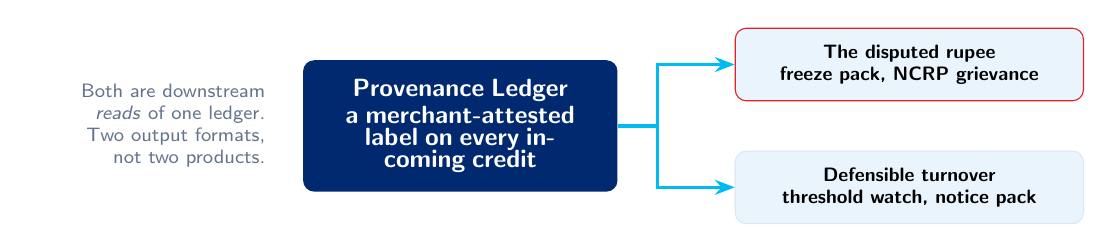
\begin{tikzpicture}[font=\scriptsize]
\node[rounded corners=4pt,fill=navy,text=white,inner sep=7pt,align=center,text width=3.5cm]
  (eng) {\bfseries\small Provenance Ledger\\[0.15em] a merchant-attested label on every incoming credit};
\node[rounded corners=4pt,fill=tint,draw=bad,inner sep=6pt,align=center,text width=4.0cm]
  (tax) at ($(eng.east)+(3.7,0.78)$) {\bfseries The disputed rupee\\ freeze pack, NCRP grievance};
\node[rounded corners=4pt,fill=tint,draw=hairline,inner sep=6pt,align=center,text width=4.0cm]
  (fra) at ($(eng.east)+(3.7,-0.78)$) {\bfseries Defensible turnover\\ threshold watch, notice pack};
\draw[-{Stealth[length=2.5mm]},ptmcyan,line width=1.3pt] (eng.east) -- ++(0.5,0) |- (tax.west);
\draw[-{Stealth[length=2.5mm]},ptmcyan,line width=1.3pt] (eng.east) -- ++(0.5,0) |- (fra.west);
\node[anchor=east,text width=2.9cm,align=right,text=muted] at ($(eng.west)+(-0.35,0)$)
  {Both are downstream \emph{reads} of one ledger. Two output formats, not two products.};
\end{tikzpicture}
\end{center}
\vspace{0.1cm}
\begin{center}
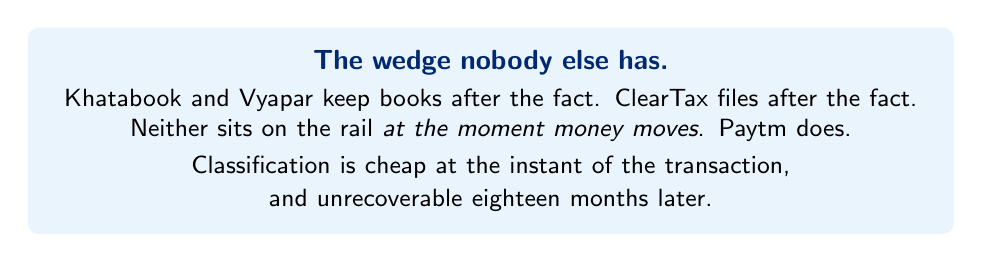
\begin{tikzpicture}\node[rounded corners=4pt,fill=tint,inner sep=8pt,text width=11.2cm,align=center]{
{\bfseries\color{navy}The wedge nobody else has.}\\[0.25em]
\small Khatabook and Vyapar keep books after the fact. ClearTax files after the fact.\\
Neither sits on the rail \emph{at the moment money moves}. Paytm does.\\[0.25em]
\small Classification is cheap at the instant of the transaction,\\ and unrecoverable eighteen months later.
};\end{tikzpicture}
\end{center}
\note{{\color{navy}\bfseries\normalsize 6.~The insight}\par\vspace{0.55em}\textbf{0:40 --- why this is one product, not two.}
\\[0.4em]
Say: \emph{``Most teams would build the fraud tool or the tax tool. They are the
same engine.''} Both are downstream reads of one ledger --- two output formats,
and the freeze pack is the one we lead with.
\\[0.4em]
Then the wedge, and say it slowly because it is the defensible-moat answer:
Khatabook and Vyapar keep books after the fact, ClearTax files after the fact.
Neither sits on the rail at the moment money moves. \textbf{Paytm does.}
\\[0.4em]
Landing line: classification is cheap and accurate at the instant of the
transaction, and unrecoverable eighteen months later when the notice arrives.}
\end{frame}

% ============================================================ 7. THE ENGINE
\begin{frame}{The engine}{Eight tags, one tap}
\vspace{0.15cm}
\begin{columns}[T]
\begin{column}{0.45\textwidth}
{\color{navy}\bfseries\small Every incoming credit gets one tag}\\[0.4em]
{\scriptsize
\begin{tabular}{@{}ll@{}}
\texttt{taxable\_supply}    & ordinary sale \\
\texttt{exempt\_supply}     & vegetables, milk, loose rice \\
\texttt{personal\_transfer} & spouse, parent, sibling \\
\texttt{inter\_account}     & her own money \\
\texttt{refund\_reversal}   & money back from a vendor \\
\texttt{duplicate}          & paid twice, one refunded \\
\texttt{non\_business}      & loan, chit payout, gift \\
{\color{bad}\texttt{unclassified}} & {\color{bad}not enough signal: ask her} \\
\end{tabular}}
\\[0.75em]
{\scriptsize\color{muted}98.6\% are ordinary sales, settled by rules. The agent reasons only about the 1.4\% that need judgement.}
\end{column}
\begin{column}{0.51\textwidth}
\card{6.6cm}{{\bfseries\color{navy}The agent proposes. The merchant attests.}\\[0.4em]
\scriptsize You cannot infer \qm{my husband sent this} from a QR payment. The agent proposes a tag \emph{with its reason}; she confirms with one tap, in Kannada, batched daily.\\[0.45em]
\scriptsize Not a fallback. A ledger she attested \emph{at the time} survives a hearing. An algorithm's guess, made under duress a year later, does not.}
\\[0.55em]
\hspace{0.15cm}\begin{minipage}{6.6cm}
{\bfseries\color{navy}\small Budget: at most 3 questions a day.}\\[0.15em]
{\scriptsize\color{muted}Over a simulated year: \hi{189 questions, median 1.3 a day}. Ask more and the product is dead.}
\end{minipage}
\end{column}
\end{columns}
\note{{\color{navy}\bfseries\normalsize 7.~The engine}\par\vspace{0.55em}\textbf{0:45 --- the mechanism. Do not read the tag list.}
\\[0.4em]
Gesture at the eight tags, say ``eight labels, every incoming credit gets one,''
and move to the right-hand card, which is the real content.
\\[0.4em]
\textbf{The line that matters:} you cannot infer ``my husband sent this'' from a
QR payment. So the agent proposes a tag \emph{with its reason} and she confirms
with one tap. This is not a fallback --- a ledger she attested contemporaneously
survives a hearing; an algorithm's guess produced under duress a year later does not.
\\[0.4em]
Then the budget: at most three questions a day, and we measured 189 across a
year, median 1.3. Ask more than that and the product is dead.
\\[0.4em]
If asked about cost: 98.6\% are ordinary sales settled by rules. The model only
sees the 1.4\% that need judgement.}
\end{frame}

% ============================================================ 8. PRODUCT
\begin{frame}{What the merchant sees}
\vspace{-0.1cm}
\begin{center}
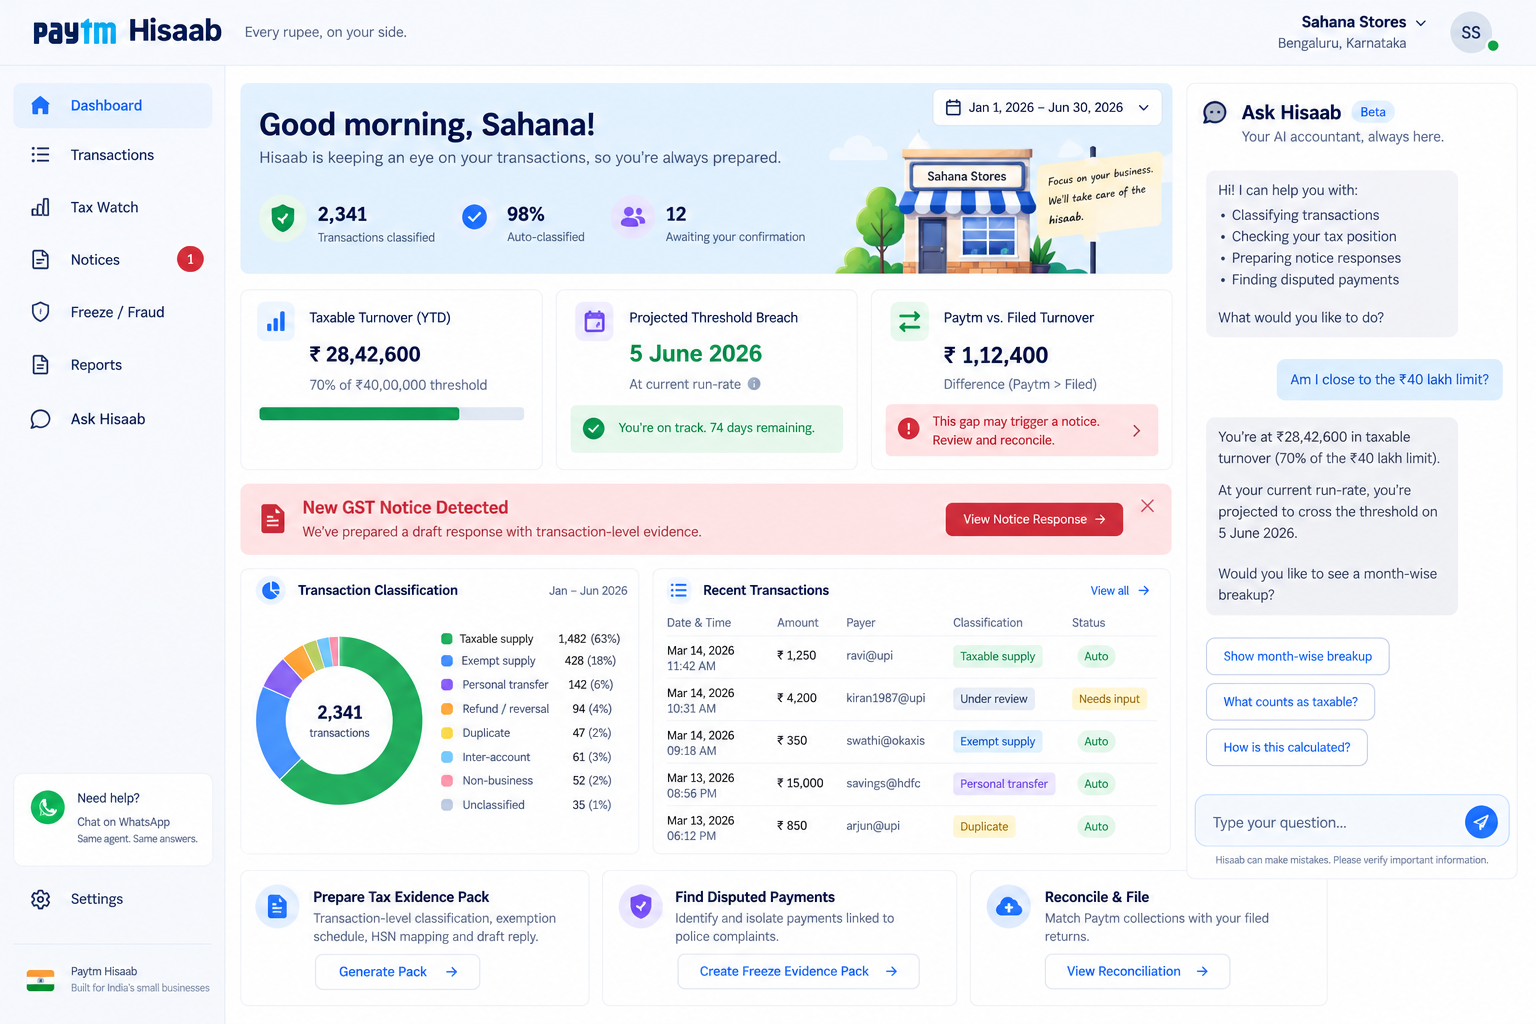
\includegraphics[width=\textwidth,height=0.70\textheight,keepaspectratio]{Paytm-Hisaab_website_look.png}
\end{center}
\vspace{0.1cm}
\hspace{0.05cm}{\scriptsize\color{muted}One surface: what every payment was classified as, how close she is to the threshold, and the packs. The same agent runs on WhatsApp, where she actually is.}
\note{{\color{navy}\bfseries\normalsize 8.~What the merchant sees}\par\vspace{0.55em}\textbf{0:20 --- a glance slide. Do not tour the UI.}
\\[0.4em]
One sentence: everything classified, how close she is to the threshold, and the
packs, on one surface.
\\[0.4em]
Then the WhatsApp point --- the same agent, where she actually is --- and advance.
\\[0.4em]
If someone asks whether this is built: the chat and the tools are live; this
screen is the product surface we are designing toward.}
\end{frame}

% ============================================================ 9. ARCHITECTURE
\begin{frame}{Built on Phinite}{Two agent graphs, four agents, ten deterministic skills}
\vspace{0.15cm}
\begin{columns}[T]
\begin{column}{0.53\textwidth}
{\scriptsize
\begin{tabular}{@{}L{1.75cm}L{4.7cm}@{}}
\multicolumn{2}{@{}l}{\color{navy}\bfseries\small hisaab-watch \;\scriptsize(autonomous: cron + API)}\\
\midrule
Provenance & proposes a tag and a reason for the hard credits \\
Evidence   & assembles packs: freeze evidence, then exemption schedules and HSN \\
\addlinespace[0.6em]
\multicolumn{2}{@{}l}{\color{navy}\bfseries\small hisaab-merchant \;\scriptsize(conversational: chat)}\\
\midrule
Merchant   & the conversation: attestation, alerts, Kannada \\
Escalation & decides when to stop and route to a human CA \\
\bottomrule
\end{tabular}}
\\[0.75em]
{\scriptsize\color{muted}The nightly pass writes its queue to the ledger; the chat reads it when she opens it. Deliberately \emph{not} a graph-to-graph call: a queue that outlives either run is what makes the handoff robust.}
\end{column}
\begin{column}{0.44\textwidth}
\card{5.7cm}{{\bfseries\color{navy}Permissions are the product}\\[0.4em]
\scriptsize Provenance proposes, \red{never commits}.\\[0.25em]
\scriptsize Merchant is the \emph{only} agent that can commit a tag.\\[0.25em]
\scriptsize Evidence is \red{read-only}. It cannot edit a classification to make a pack look better.\\[0.25em]
\scriptsize Escalation can \red{halt} any pack; a human approves.}
\\[0.5em]
\hspace{0.1cm}\begin{minipage}{5.7cm}{\scriptsize\color{muted}Ten tools run live against a hosted service. Every number in a pack traces back, in the trace, to the credit and the attestation behind it.}\end{minipage}
\end{column}
\end{columns}
\note{{\color{navy}\bfseries\normalsize 9.~Built on Phinite}\par\vspace{0.55em}\textbf{0:40 --- for the technical judges.}
\\[0.4em]
Two agent graphs, not four loose agents: \texttt{hisaab-watch} runs autonomously on
cron, \texttt{hisaab-merchant} is the conversation. The nightly pass writes a queue;
the chat reads it when she opens it --- deliberately not a graph-to-graph call,
because a queue that outlives either run is what makes the handoff robust.
\\[0.4em]
\textbf{Spend your time on the right-hand card.} The strongest line in it:
the Evidence agent is read-only --- \emph{the agent that builds the defence cannot
edit the evidence.} And only the Merchant agent can commit an attested tag.
\\[0.4em]
Those are enforced as Phinite tool policies, not conventions, and a denied call
shows up in the trace.}
\end{frame}

% ============================================================ 10. DESIGN DECISIONS
\begin{frame}{Four decisions that make it defensible}
\vspace{0.3cm}
\begin{columns}[T]
\begin{column}{0.48\textwidth}
\card{6.0cm}{{\bfseries\color{navy}1. Arithmetic lives in skills, not the model}\\[0.35em]
\scriptsize Turnover, projections and apportionment are deterministic Python: versioned, testable, traceable. Wrapping arithmetic in an LLM is the standard tell, and the trace would show it.}
\\[0.35em]
\card{6.0cm}{{\bfseries\color{navy}3. Refusing to guess is a feature}\\[0.35em]
\scriptsize An \texttt{unclassified} credit routed to the merchant costs one tap. A confident wrong tag inside an evidence pack is a catastrophe. We report the refusal rate honestly.}
\end{column}
\begin{column}{0.48\textwidth}
\card{6.0cm}{{\bfseries\color{navy}2. Attestation is the promotion boundary}\\[0.35em]
\scriptsize Nothing enters a production pack that the merchant has not confirmed. Sandbox to UAT to prod, with her tap as the gate.}
\\[0.35em]
\card{6.0cm}{{\bfseries\color{navy}4. Ground truth, so accuracy is a number}\\[0.35em]
\scriptsize We simulated a year of a shop's life from a known process, split into what Paytm can see and what really happened. Agents read only the visible half, which is why we quote error bars instead of vibes.}
\end{column}
\end{columns}
\note{{\color{navy}\bfseries\normalsize 10.~Four decisions}\par\vspace{0.55em}\textbf{0:35 --- the slide that separates you from a demo.}
\\[0.4em]
Lead with \#1: all arithmetic is deterministic Python, not model output. Wrapping
arithmetic in an LLM is the standard tell, and the trace would show it.
\\[0.4em]
Then \#3: refusing to guess is a feature. An \texttt{unclassified} credit costs one
tap; a confident wrong tag inside an evidence pack is a catastrophe.
\\[0.4em]
Skim \#2 and \#4 --- one clause each. \#4 is worth a beat if the room is technical:
we generated ground truth, so accuracy is a number instead of a claim.}
\end{frame}

% ============================================================ 11. DEMO / ATTESTATION
\begin{frame}{Demo $\cdot$ Sahana Stores, Jayanagar}{An ordinary Tuesday, before anything goes wrong}
\vspace{0.1cm}
\begin{columns}[T]
\begin{column}{0.48\textwidth}
{\scriptsize\color{muted}Tuesday 10 March. Thirty-nine credits came in over the weekend. The agent asks about \hi{three}.}
\\[0.4em]
\card{5.9cm}{{\kn\scriptsize ಭಾನುವಾರ ರಾತ್ರಿ ₹15,000. ನಿಮ್ಮ ಸ್ವಂತ ಹಣವೇ?}\\[0.25em]
{\color{muted}\scriptsize \qm{₹15,000 at 11:04pm Sunday, from your savings account. Your own money?}}\\[0.35em]
{\scriptsize\color{navy}\fbox{\kn ಹೌದು}\;\fbox{\kn ಇಲ್ಲ}}}
\\[0.4em]
{\scriptsize $\cdot$\; ₹7,500 from her husband, scanned at the shop QR\\[0.25em]
$\cdot$\; ₹4,850 from Raghu Shetty, who has bought twice before. A real sale, and the agent \emph{asks} rather than assumes.}
\\[0.4em]
{\scriptsize\color{muted}The other thirty-six settle silently, and a ₹23 payment nobody can place is left alone.}
\end{column}
\begin{column}{0.48\textwidth}
\ocard{amber}{6.1cm}{{\bfseries\color{amber}And yes, two of those three should not be there}\\[0.35em]
\scriptsize A business QR is not for personal money, and the terms say so. It arrives anyway: family, own top-ups, a chit payout. The rule does not prevent it. It only means \emph{nobody keeps a record of it.}}
\\[0.45em]
{\scriptsize Paytm already reads the signals: channel, linked VPAs, payer history. What no system has is the \hi{merchant's own answer}, given at the time, in her language, and kept.}
\\[0.45em]
{\scriptsize That record is what the next two slides are built from: first for the police, then for the department.}
\end{column}
\end{columns}
\note{{\color{navy}\bfseries\normalsize 11.~Demo --- an ordinary Tuesday (beat 1)}\par\vspace{0.55em}\textbf{0:45 --- or hand over to the live demo here.}
\\[0.4em]
Thirty-nine credits came in over the weekend, the agent asks about \textbf{three}.
Read the Kannada line if you can; otherwise read the gloss under it.
\\[0.4em]
\textbf{Do not hide from the right-hand card --- lead with it.} The mid-review
point was that personal money is not allowed on a business QR. Correct, and we say
so on the slide. The argument is that the rule does not stop it, it only means no
one records it, and an unrecorded credit is what an authority later reads as income.
\\[0.4em]
\textbf{Second half of that card matters just as much.} We are not claiming Paytm
does nothing. It already reads channel, linked VPAs and payer history. What no
system has is her own answer, captured while it is still knowable. That is the
product, and it is a smaller, truer claim than the one we started with.
\\[0.4em]
\textbf{Before going on stage:} confirm the attestation queue is whole ---
\texttt{pending\_total} must be 3. A rehearsal that taps through this beat spends the
queue, and Render needs a clear-cache redeploy to restore it.}
\end{frame}

% ============================================================ 12. DEMO / THE FREEZE
\begin{frame}{Demo $\cdot$ The emergency}{The account is frozen at 09:30 and the supplier payment is due}
\vspace{0.2cm}
\begin{columns}[T]
\begin{column}{0.46\textwidth}
{\scriptsize She sold someone 12kg of onions. That customer was three layers downstream of a fraud victim. She is not named in the FIR, which was filed in another state, and \hi{339 payments} came in that week.}
\\[0.5em]
\card{5.8cm}{{\bfseries\color{navy}The agent isolates it}\\[0.35em]
\scriptsize ₹4,200 on 21 March at 19:47, till POS01. Matched by UTR \emph{and independently} by amount and date.\\[0.3em]
\scriptsize The sale record comes with it: the POS bill, the items, the till and the minute.}
\end{column}
\begin{column}{0.49\textwidth}
\ocard{amber}{6.1cm}{{\bfseries\color{amber}And the decoy it did not choose}\\[0.35em]
\scriptsize A \emph{second} ₹4,200 that same week, from a regular customer. Listed in the pack, and explicitly \emph{not} named as the disputed one. Only the date separates them.}
\\[0.5em]
{\scriptsize Then it drafts the NCRP-CFCFRMS grievance, citing the judgments that only the \emph{disputed amount} should be lien-marked, not the whole account.}
\\[0.5em]
{\scriptsize\color{bad}\bfseries It never asserts that she is innocent.}\\[0.1em]
{\scriptsize\color{muted}Some frozen accounts genuinely are mule accounts. The agent assembles evidence; a human decides. Escalation holds the pack for approval.}
\end{column}
\end{columns}
\note{{\color{navy}\bfseries\normalsize 12.~Demo --- the emergency (beat 4)}\par\vspace{0.55em}\textbf{0:50 --- this is now the lead case. Give it the most time of the three.}
\\[0.4em]
Set the stakes in one sentence: account frozen at half nine, supplier payment due,
339 payments came in that week, and she is not named in the FIR.
\\[0.4em]
\textbf{Why this one leads.} She did nothing wrong and there is no rule she broke.
She sold onions to a customer who turned out to be laundering. Every objection
available against the tax case --- she should not have taken personal money on that
QR, she should have registered --- has no purchase here at all.
\\[0.4em]
The agent isolates ₹4,200 by UTR \emph{and independently} by amount and date, and
brings the POS bill with it --- the items, till POS01, 19:47.
\\[0.4em]
\textbf{The decoy is the point.} A second ₹4,200 that same week from a regular
customer, listed in the pack and explicitly not chosen. Anyone can match an amount;
the pack shows its work.
\\[0.4em]
Finish on the red line: it never asserts she is innocent. Some frozen accounts
genuinely are mule accounts. We assemble evidence; a human decides, and Escalation
holds the pack for approval.}
\end{frame}

% ============================================================ 13. DEMO / TAX
\begin{frame}{Demo $\cdot$ The warning, and the notice}{The same ledger, read for the other authority}
\vspace{0.15cm}
\begin{columns}[T]
\begin{column}{0.38\textwidth}
{\scriptsize\color{muted}Replayed as of 31 January:}
\\[0.35em]
\ocard{good}{4.8cm}{{\bfseries\color{ink}\scriptsize\qm{At your current rate you cross ₹40 lakh around {\color{bad}14 March}. You will need to register.}}\\[0.35em]
{\scriptsize\color{muted}\grn{43 days of warning}, and the date is computed, not typed.}}
\\[0.45em]
{\scriptsize\color{bad}\bfseries This beat is what makes the pitch safe.}\\[0.1em]
{\scriptsize\color{muted}Its first act on the tax side is telling her to register.}
\end{column}
\begin{column}{0.58\textwidth}
{\scriptsize\color{muted}Then the notice arrives, claiming {\color{bad}\bfseries ₹60.98L} of turnover:}
\\[0.3em]
{\scriptsize
\begin{tabular}{@{}lr@{\hskip 1.2em}l@{}}
\multicolumn{2}{@{}l}{\color{navy}\bfseries Aggregate turnover \quad ₹42.2L} & \sub{within \grn{1.6\%} of truth} \\
\midrule
Exempt supplies      & ₹31.3L & \sub{vegetables, loose rice} \\
Taxable supplies     & ₹10.9L & \sub{branded goods, oil, soap} \\
\addlinespace[0.45em]
\multicolumn{2}{@{}l}{\color{navy}\bfseries Not turnover at all \quad ₹18.8L} & \sub{every line traced} \\
\midrule
Her own accounts     & ₹7.4L & \sub{top-ups before supplier runs} \\
Family               & ₹6.1L & \sub{spouse, parent, in-law} \\
Loans, chit, gifts   & ₹4.3L & \sub{chit payout, festival gifts} \\
Refunds, duplicates  & ₹1.0L & \sub{crate returns, double-taps} \\
\bottomrule
\end{tabular}}
\\[0.45em]
{\scriptsize And it says plainly: \hi{the claim is wrong, and you \emph{did} cross ₹40 lakh on 14 March. You must register.}}
\end{column}
\end{columns}
\note{{\color{navy}\bfseries\normalsize 13.~Demo --- the warning and the notice (beats 2 and 3)}\par\vspace{0.55em}\textbf{0:50 --- two tax beats on one slide, deliberately compressed.}
\\[0.4em]
Left: replayed as of 31 January, the agent says she crosses ₹40 lakh around
14 March. \textbf{Say the red line out loud} --- its first act on the tax side is
telling her she owes a registration. That is what stops the room turning hostile.
\\[0.4em]
Right: the notice claims ₹60.98 lakh, and the pack answers it line by line, every
figure traceable to transaction IDs. Then the honest half:
\textbf{the claim is wrong, and she did cross ₹40 lakh, and she must register.}
\\[0.4em]
\textbf{If a judge diffs this against slide 5:} slide 5 shows seeded truth
(₹42.9L), this shows what our system computed (₹42.2L). The 1.6\% between them
\emph{is} the accuracy claim --- say that, do not hedge.
\\[0.4em]
\textbf{If pushed on the personal and own-account lines:} same answer as slide 11.
Those credits should not be on a business QR, they are there anyway, and the
alternative to classifying them is letting them be read as income.}
\end{frame}

% ============================================================ 14. NUMBERS
\begin{frame}{What we can actually prove}{One merchant, one year, 13,267 credits, scored against seeded truth}
\vspace{0.45cm}
\begin{columns}[T]
\begin{column}{0.33\textwidth}
\begin{center}\bignum{1.6\%}{error on aggregate turnover\\ (taxable share within 1\%)}\end{center}
\vspace{0.55cm}
\begin{center}\bignum{43 days}{of warning before the\\ threshold crossing}\end{center}
\end{column}
\begin{column}{0.33\textwidth}
\begin{center}\bignum{1.3 a day}{median questions asked.\\ 189 in a year, never over 3}\end{center}
\vspace{0.55cm}
\begin{center}\bignum{zero}{credits left untagged\\ across the whole year}\end{center}
\end{column}
\begin{column}{0.30\textwidth}
\card{3.8cm}{{\bfseries\color{navy}The honest baseline}\\[0.35em]
\scriptsize A 50-line rules-only classifier gets 99.3\% on sale vs not-a-sale, but catches only \red{77.8\%} of non-sale credits.\\[0.3em]
\scriptsize That residue alone puts two eval merchants on the \emph{wrong side} of ₹40L.\\[0.3em]
\scriptsize Closing it is what the agent plus one tap is for.}
\end{column}
\end{columns}
\vspace{0.45cm}
\hspace{0.1cm}{\scriptsize\color{muted}She corrected the agent 52 times that year. Those corrections are the ledger's strongest evidence, not its failures.}
\note{{\color{navy}\bfseries\normalsize 14.~What we can actually prove}\par\vspace{0.55em}\textbf{0:30 --- do not read all four. Pick two.}
\\[0.4em]
Lead with \textbf{1.6\%} error on turnover and \textbf{1.3 questions a day}. The
other two are there to be read, not narrated.
\\[0.4em]
\textbf{The credibility move is the box on the right} --- volunteer the weakness
before anyone finds it. A rules-only baseline gets 99.3\% on sale vs not-a-sale
but catches only 77.8\% of non-sale credits, and that residue alone puts two eval
merchants on the wrong side of ₹40 lakh. Closing it is what the agent plus one tap is for.
\\[0.4em]
Last line if you have the beat: she corrected the agent 52 times that year, and
those corrections are the ledger's strongest evidence, not its failures.}
\end{frame}

% ============================================================ 15. CLOSE
\begin{frame}{The line we do not cross}{Accuracy, not minimisation}
\vspace{0.3cm}
\begin{columns}[T]
\begin{column}{0.52\textwidth}
{\scriptsize
$\cdot$\; We \hi{never assert innocence} on a freeze. Some accounts really are mule accounts. We assemble evidence; a human decides.\\[0.5em]
$\cdot$\; We \hi{file nothing} with any authority. Artefacts only; the merchant or their CA files.\\[0.5em]
$\cdot$\; We compute what she \hi{genuinely owes} and say so plainly, including \qm{you crossed the threshold, you must register.}\\[0.5em]
$\cdot$\; We \hi{never assert a final liability}. We compute, show the workings, and route to a CA.\\[0.5em]
$\cdot$\; A business QR is \hi{not for personal money}. We do not excuse it. We record it, so it is not read as income.}
\end{column}
\begin{column}{0.44\textwidth}
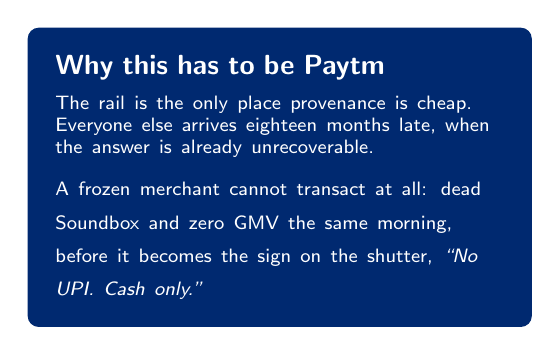
\begin{tikzpicture}\node[rounded corners=4pt,fill=navy,text=white,inner sep=10pt,text width=5.7cm,align=left]{
{\bfseries Why this has to be Paytm}\\[0.45em]
\scriptsize The rail is the only place provenance is cheap. Everyone else arrives eighteen months late, when the answer is already unrecoverable.\\[0.45em]
\scriptsize A frozen merchant cannot transact at all: dead Soundbox and zero GMV the same morning, before it becomes the sign on the shutter, \emph{\qm{No UPI. Cash only.}}
};\end{tikzpicture}
\end{column}
\end{columns}
\vspace{0.4cm}
\begin{center}
{\large\color{navy}\bfseries Paytm Hisaab}\quad{\color{muted}every rupee, on your side.}
\end{center}
\note{{\color{navy}\bfseries\normalsize 15.~The line we do not cross}\par\vspace{0.55em}\textbf{0:30 --- the non-negotiables, fast, then land.}
\\[0.4em]
Run the five bullets at pace. The one to hit is the first: we never assert
innocence on a freeze. The last is the mid-review answer, on the slide on purpose.
\\[0.4em]
Then the navy box: provenance is cheap only on the rail, and a frozen merchant
stops transacting the same morning.
\\[0.4em]
Final line, unhurried: \emph{``Paytm Hisaab. Every rupee, on your side.''} Stop talking.
\\[0.5em]
{\scriptsize
{\color{navy}\bfseries --- Q\&A prep ---}
\\[0.3em]
\textbf{``Merchants may not take personal money on a business QR.''} Correct, and
slide 11 says so before you have to. It arrives anyway, and the alternative to
recording it is letting an authority read it as income. We are not defending the
behaviour --- we are refusing to let it become a liability.
\\[0.3em]
\textbf{``Paytm already tags transactions.''} It does, and we build on that rather
than around it: channel, linked VPAs and payer history feed the rules layer. What
no tag carries is her attestation --- the part an authority accepts, and the only
part she alone can give.
\\[0.3em]
\textbf{``No return mismatch?''} That check needs a \emph{registered} composition
dealer who filed a CMP-08 to disagree with. Ours is unregistered, which is why she
gets a notice at all; the eval split has one with four quarters seeded.
\\[0.3em]
\textbf{``Exempt vs taxable on a QR sale?''} Not per payment. We apportion by value
from that shop's own POS-billed ratio and label it an estimate. Labelling each sale
by its majority side understated taxable turnover threefold.
\\[0.3em]
\textbf{``Four LLM calls in a trenchcoat?''} Everything deterministic is a skill and
four agents is the ceiling. If twenty lines of Python replaces an agent, it should
have been a skill --- the trace shows which is which.
\\[0.3em]
\textbf{``No standing with the police.''} Agreed: Paytm supplies, the merchant
files. By design. Cash sales are real, out of scope, and on the slide.}}
\end{frame}

\end{document}
"
%                                                     -> speaker notes, one page per slide
%
% Speaker notes live in the \note{} after each frame, so they cannot drift
% out of sync with the slides. Build both with: ./build.sh
%
% Fonts: Segoe UI + Nirmala UI (both ship with Windows). On another OS the
% deck still builds -- it falls back to the default sans and drops the
% Kannada styling.
\documentclass[aspectratio=169,10pt]{beamer}

\usepackage{fontspec}
\usepackage{tikz}
\usepackage{booktabs}
\usepackage{array}
\newcolumntype{L}[1]{>{\raggedright\arraybackslash}p{#1}}
\usepackage{graphicx}
\usetikzlibrary{calc,positioning,arrows.meta}

\graphicspath{{./}{../}}

% ---------- fonts ----------
\IfFontExistsTF{Segoe UI}{\setsansfont{Segoe UI}}{}
\IfFontExistsTF{Nirmala UI}{%
  \newfontfamily\kn[Script=Kannada]{Nirmala UI}}{%
  \newcommand{\kn}{}}
\renewcommand{\familydefault}{\sfdefault}

% ragged, unhyphenated text inside the narrow cards
\hyphenpenalty=10000
\exhyphenpenalty=10000
\emergencystretch=3em
\hbadness=10000

% ---------- palette (taken from the product mock) ----------
\definecolor{navy}{HTML}{002970}
\definecolor{ptmcyan}{HTML}{00BAF2}
\definecolor{ink}{HTML}{0F172A}
\definecolor{muted}{HTML}{64748B}
\definecolor{good}{HTML}{15803D}
\definecolor{bad}{HTML}{DC2626}
\definecolor{amber}{HTML}{B45309}
\definecolor{tint}{HTML}{EAF4FD}
\definecolor{hairline}{HTML}{DBE7F3}

% ---------- theme ----------
\usetheme{default}
\usecolortheme{default}
\setbeamertemplate{navigation symbols}{}
\setbeamersize{text margin left=0.85cm,text margin right=0.85cm}
\setbeamercolor{normal text}{fg=ink,bg=white}
\setbeamercolor{frametitle}{fg=navy}
\setbeamercolor{structure}{fg=navy}
\setbeamerfont{frametitle}{size=\large,series=\bfseries}
\setbeamerfont{framesubtitle}{size=\scriptsize}
\setbeamercolor{framesubtitle}{fg=muted}
\setbeamertemplate{frametitle}{%
  \vspace{0.30cm}%
  \usebeamerfont{frametitle}\usebeamercolor[fg]{frametitle}\insertframetitle%
  \ifx\insertframesubtitle\empty\else{\\[-0.15em]\usebeamerfont{framesubtitle}\usebeamercolor[fg]{framesubtitle}\insertframesubtitle}\fi%
  \\[0.1em]{\color{ptmcyan}\rule{1.2cm}{2pt}}\par\vspace{-0.15em}%
}
\setbeamertemplate{footline}{%
  \hbox{\begin{beamercolorbox}[wd=\paperwidth,ht=1.9ex,dp=1.1ex,leftskip=0.85cm,rightskip=0.85cm]{}%
  {\scriptsize\color{muted}Paytm Hisaab\hfill\insertframenumber}%
  \end{beamercolorbox}}%
}
\setbeamerfont{itemize/enumerate body}{size=\normalsize}

% ---------- helpers ----------
\newcommand{\hi}[1]{{\color{navy}\bfseries #1}}
\newcommand{\red}[1]{{\color{bad}\bfseries #1}}
\newcommand{\grn}[1]{{\color{good}\bfseries #1}}
\newcommand{\sub}[1]{{\color{muted}#1}}
\newcommand{\qm}[1]{``#1''}
\newcommand{\bignum}[2]{{\color{navy}\fontsize{22}{24}\selectfont\bfseries #1}\\[0.1em]{\scriptsize\color{muted}#2}}
% a soft rounded card:  \card{width}{body}
\newcommand{\card}[2]{\begin{tikzpicture}%
  \node[rounded corners=4pt,fill=tint,inner sep=8pt,text width=#1,align=left]{#2};%
  \end{tikzpicture}}
% an outlined card:  \ocard{colour}{width}{body}
\newcommand{\ocard}[3]{\begin{tikzpicture}%
  \node[rounded corners=4pt,fill=white,draw=#1,line width=0.9pt,inner sep=8pt,text width=#2,align=left]{#3};%
  \end{tikzpicture}}

% ---------- presenter build ----------
% Set after every colour and template above, so the composed notes page keeps
% the deck's own colours:
%   xelatex -jobname=hisaab-pitch-notes "\def\shownotes{1}% Paytm Hisaab -- buildathon pitch deck
%
% Compile with XeLaTeX (needed for the rupee sign and the Kannada line):
%
%   cd pitch
%   xelatex hisaab-pitch.tex                          -> hisaab-pitch.pdf  (slides)
%   xelatex -jobname=hisaab-pitch-notes "\def\shownotes{1}\input{hisaab-pitch.tex}"
%                                                     -> speaker notes, one page per slide
%
% Speaker notes live in the \note{} after each frame, so they cannot drift
% out of sync with the slides. Build both with: ./build.sh
%
% Fonts: Segoe UI + Nirmala UI (both ship with Windows). On another OS the
% deck still builds -- it falls back to the default sans and drops the
% Kannada styling.
\documentclass[aspectratio=169,10pt]{beamer}

\usepackage{fontspec}
\usepackage{tikz}
\usepackage{booktabs}
\usepackage{array}
\newcolumntype{L}[1]{>{\raggedright\arraybackslash}p{#1}}
\usepackage{graphicx}
\usetikzlibrary{calc,positioning,arrows.meta}

\graphicspath{{./}{../}}

% ---------- fonts ----------
\IfFontExistsTF{Segoe UI}{\setsansfont{Segoe UI}}{}
\IfFontExistsTF{Nirmala UI}{%
  \newfontfamily\kn[Script=Kannada]{Nirmala UI}}{%
  \newcommand{\kn}{}}
\renewcommand{\familydefault}{\sfdefault}

% ragged, unhyphenated text inside the narrow cards
\hyphenpenalty=10000
\exhyphenpenalty=10000
\emergencystretch=3em
\hbadness=10000

% ---------- palette (taken from the product mock) ----------
\definecolor{navy}{HTML}{002970}
\definecolor{ptmcyan}{HTML}{00BAF2}
\definecolor{ink}{HTML}{0F172A}
\definecolor{muted}{HTML}{64748B}
\definecolor{good}{HTML}{15803D}
\definecolor{bad}{HTML}{DC2626}
\definecolor{amber}{HTML}{B45309}
\definecolor{tint}{HTML}{EAF4FD}
\definecolor{hairline}{HTML}{DBE7F3}

% ---------- theme ----------
\usetheme{default}
\usecolortheme{default}
\setbeamertemplate{navigation symbols}{}
\setbeamersize{text margin left=0.85cm,text margin right=0.85cm}
\setbeamercolor{normal text}{fg=ink,bg=white}
\setbeamercolor{frametitle}{fg=navy}
\setbeamercolor{structure}{fg=navy}
\setbeamerfont{frametitle}{size=\large,series=\bfseries}
\setbeamerfont{framesubtitle}{size=\scriptsize}
\setbeamercolor{framesubtitle}{fg=muted}
\setbeamertemplate{frametitle}{%
  \vspace{0.30cm}%
  \usebeamerfont{frametitle}\usebeamercolor[fg]{frametitle}\insertframetitle%
  \ifx\insertframesubtitle\empty\else{\\[-0.15em]\usebeamerfont{framesubtitle}\usebeamercolor[fg]{framesubtitle}\insertframesubtitle}\fi%
  \\[0.1em]{\color{ptmcyan}\rule{1.2cm}{2pt}}\par\vspace{-0.15em}%
}
\setbeamertemplate{footline}{%
  \hbox{\begin{beamercolorbox}[wd=\paperwidth,ht=1.9ex,dp=1.1ex,leftskip=0.85cm,rightskip=0.85cm]{}%
  {\scriptsize\color{muted}Paytm Hisaab\hfill\insertframenumber}%
  \end{beamercolorbox}}%
}
\setbeamerfont{itemize/enumerate body}{size=\normalsize}

% ---------- helpers ----------
\newcommand{\hi}[1]{{\color{navy}\bfseries #1}}
\newcommand{\red}[1]{{\color{bad}\bfseries #1}}
\newcommand{\grn}[1]{{\color{good}\bfseries #1}}
\newcommand{\sub}[1]{{\color{muted}#1}}
\newcommand{\qm}[1]{``#1''}
\newcommand{\bignum}[2]{{\color{navy}\fontsize{22}{24}\selectfont\bfseries #1}\\[0.1em]{\scriptsize\color{muted}#2}}
% a soft rounded card:  \card{width}{body}
\newcommand{\card}[2]{\begin{tikzpicture}%
  \node[rounded corners=4pt,fill=tint,inner sep=8pt,text width=#1,align=left]{#2};%
  \end{tikzpicture}}
% an outlined card:  \ocard{colour}{width}{body}
\newcommand{\ocard}[3]{\begin{tikzpicture}%
  \node[rounded corners=4pt,fill=white,draw=#1,line width=0.9pt,inner sep=8pt,text width=#2,align=left]{#3};%
  \end{tikzpicture}}

% ---------- presenter build ----------
% Set after every colour and template above, so the composed notes page keeps
% the deck's own colours:
%   xelatex -jobname=hisaab-pitch-notes "\def\shownotes{1}\input{hisaab-pitch.tex}"
\ifdefined\shownotes
  \setbeamertemplate{note page}{%
    \usebeamercolor[fg]{normal text}%
    \vspace{0.2em}%
    {\scriptsize\color{muted}Paytm Hisaab \;$\cdot$\; speaker notes}\hfill
    {\scriptsize\color{muted}slide \insertframenumber\ of 15}\par
    \vspace{0.25em}{\color{ptmcyan}\rule{\textwidth}{1.5pt}}\par
    \vspace{0.55em}\footnotesize\raggedright\insertnote\par}
  \setbeameroption{show only notes}
\fi

\begin{document}

% ============================================================ 1. TITLE
{\setbeamertemplate{footline}{}
\begin{frame}[plain]
\vspace{0.9cm}
\begin{center}
{\fontsize{38}{42}\selectfont\bfseries\color{navy}Paytm\;\color{ink}Hisaab}\\[0.45em]
{\Large\color{muted}Every rupee, on your side.}\\[0.9em]
{\color{ptmcyan}\rule{2.8cm}{2.5pt}}\\[0.9em]
{\large\color{ink}The agent that lets a merchant account for their own money}\\[0.15em]
{\large\color{ink}when someone in authority demands an explanation.}\\[1.3em]
{\small\color{muted}Agent Labs Buildathon \;$\cdot$\; Phinite $\times$ Paytm \;$\cdot$\; Track 2: AI for Small Businesses}
\end{center}
\note{{\color{navy}\bfseries\normalsize 1.~Title}\par\vspace{0.55em}\textbf{0:10 --- open cold.} Do not read the title or the tagline off the slide.
\\[0.4em]
Say: \emph{``I want to tell you about a man in Haveri who opened an envelope.''} Then advance.
\\[0.4em]
Nothing on this slide needs explaining. The tagline lands at the end, not here.}
\end{frame}}

% ============================================================ 2. STORY
\begin{frame}{Haveri, 2025}{A vegetable vendor opens an envelope}
\vspace{0.05cm}
\begin{columns}[T]
\begin{column}{0.52\textwidth}
\vspace{0.15cm}
He sells vegetables. Vegetables are \hi{exempt} from GST.\\[0.6em]
He also took UPI, because Paytm asked him to.\\[0.6em]
Four years of credits into his account, added up and billed as income:
\begin{center}\vspace{0.1em}{\fontsize{30}{32}\selectfont\bfseries\color{bad}₹29 lakh}\end{center}
\end{column}
\begin{column}{0.44\textwidth}
\ocard{hairline}{5.4cm}{\centering
  {\color{muted}\scriptsize Within weeks, on shutters across Karnataka:}\\[0.6em]
  {\fontsize{20}{23}\selectfont\bfseries\color{ink}\qm{No UPI.\\ Cash only.}}\\[0.6em]
  {\color{muted}\scriptsize A statewide boycott, by the merchants who had just adopted it.}}
\end{column}
\end{columns}
\vspace{0.25cm}
\hspace{0.1cm}{\small\sub{Withdrawn for the traders who could \emph{show} what they sold. Most could not. And tax is no longer the only authority asking.}}
\note{{\color{navy}\bfseries\normalsize 2.~Haveri, 2025}\par\vspace{0.55em}\textbf{0:45 --- the hook. Tell it, do not summarise it.}
\\[0.4em]
Four beats, in this order: he sells vegetables; vegetables are exempt from GST;
he took UPI because \emph{we} asked him to; the department added up four years of
credits and sent him a bill for \textbf{₹29 lakh}.
\\[0.4em]
\textbf{Pause on the number.} Then the card: within weeks, shutters across Karnataka
read ``No UPI, cash only.'' Merchants we had just onboarded, boycotting the rail.
\\[0.4em]
Close on the bottom line --- the notices were withdrawn for traders who could
\emph{show} what they sold. Most could not. That verb is the whole product.
\\[0.4em]
\textbf{Then the bridge:} \emph{``and tax is no longer the only authority asking.''}
That sentence is doing the repositioning --- Haveri is not a tax story here, it is
the moment taking digital money became a liability. The sharper version of it is
two slides away.
\\[0.4em]
\textbf{Do not say this is happening right now.} It is 2025. The next slide is
what makes it current, and a judge who knows the episode will respect the distinction.}
\end{frame}

% ============================================================ 3. STILL HAPPENING
\begin{frame}{And this is not a 2025 story}{CAclubindia, last updated 02 September 2026: ten days ago}
\vspace{0.1cm}
\begin{center}

\includegraphics[width=12.4cm]{gst-notices-2026.png}
\end{center}
\vspace{0.35cm}
\card{13.1cm}{\scriptsize\qm{During August 2026, the GST Department issued a significant number of notices covering different financial years and involving a wide range of issues\ldots\ They covered matters such as ITC mismatches, ineligible credit, \hi{differences in turnover}, wrong GST classification or rate, \hi{exemption claims}, Reverse Charge Mechanism\ldots}}
\vspace{0.3cm}

\hspace{0.1cm}{\small Those two categories are the whole content of an evidence pack. And this is the \emph{slower} of the two authorities. The other one freezes the account first.}
\note{{\color{navy}\bfseries\normalsize 3.~And this is not a 2025 story}\par\vspace{0.55em}\textbf{0:25 --- fast. This slide exists to kill one objection.}
\\[0.4em]
Say: \emph{``That was last year. This was published ten days ago.''}
\\[0.4em]
Do not read the quote. Point at the two bolded phrases only ---
\textbf{differences in turnover} and \textbf{exemption claims} --- and say those
two categories are the entire content of what we build.
\\[0.4em]
\textbf{Land on the last line and move.} It is the handoff into the police
slide: this is the slower authority. The other one freezes first and asks
afterwards. Do not linger here --- tax is no longer the headline.}
\end{frame}

% ============================================================ 4. THE TRAP
\begin{frame}{Every rupee a merchant receives is now evidence}{Today it is only ever used against them}
\vspace{0.05cm}
\begin{columns}[T]
\begin{column}{0.47\textwidth}
\ocard{bad}{6.0cm}{{\bfseries\color{bad}The cyber-crime police}\\[0.35em]
\scriptsize Fraud money layers through accounts within minutes. The shop at the end of the chain, the one that sold someone a watermelon, is frozen. It did nothing wrong, is not named in the FIR, and finds out when a payment declines.}
\end{column}
\begin{column}{0.47\textwidth}
\card{6.1cm}{{\bfseries\color{navy}The tax department}\\[0.35em]
\scriptsize Compares UPI collections against filed returns and bills the difference. Registered traders too, with QR, wallet, card and cash deposits all in scope.}
\end{column}
\end{columns}
\vspace{0.4cm}
\begin{center}
{\large Both demand the same artefact: \hi{what was each rupee, actually?}}\\[0.3em]
{\small\color{muted}Paytm already sees more of this than anyone. What is missing is the \emph{merchant's own answer}, captured when it is still knowable.}
\end{center}
\vspace{0.15cm}
{\color{hairline}\hrule height 1pt}
\vspace{0.35em}
\hspace{0.05cm}{\scriptsize\bfseries\color{bad}What it costs Paytm:}~{\scriptsize a frozen merchant stops transacting that morning. A frightened one takes the QR down for good. Dead Soundbox, zero GMV, no lending origination.}
\note{{\color{navy}\bfseries\normalsize 4.~Every rupee is now evidence}\par\vspace{0.55em}\textbf{0:40 --- two authorities, one unanswerable question.}
\\[0.4em]
\textbf{Left card first and give it the time.} Fraud money layers within minutes,
and the shop at the end of the chain, \emph{the one that sold someone a watermelon},
gets frozen. It did nothing wrong, it is not named in the FIR, and it finds out
when a payment declines. Use the watermelon.
\\[0.4em]
Right card briskly: the department reconciles collections against filed returns
and bills the difference. One sentence, then move.
\\[0.4em]
Then the pivot: both demand the same artefact --- what was each rupee, actually.
\\[0.4em]
\textbf{Say the grey line as written.} We do \emph{not} claim Paytm does nothing
with this data --- it tags plenty. The gap is the merchant's own answer, captured
when it is still knowable. Claiming otherwise in this room gets corrected.
\\[0.4em]
\textbf{Slow down for the red line.} This is the business case, not a footnote:
a frozen merchant stops transacting that morning, a frightened one takes the QR
down for good. Dead Soundbox, zero GMV, no lending origination.}
\end{frame}

% ============================================================ 5. THE BAR
\begin{frame}{Gross credits are not turnover}{One shop, one year, ₹60.98 lakh of credits}
\vspace{0.1cm}
\begin{center}
\begin{tikzpicture}[x=1cm,y=1cm]
% --- what the notice counts
\node[anchor=west,font=\scriptsize\bfseries,text=bad] at (-0.05,1.80) {WHAT THE NOTICE COUNTS AS TURNOVER};
\fill[bad!85,rounded corners=2pt] (0,1.06) rectangle (11.4,1.60);
\node[font=\small\bfseries,text=white] at (5.7,1.33) {₹60.98 lakh};

% --- what actually happened   (1 lakh = 0.18696 cm, so the bars are the same length)
\node[anchor=west,font=\scriptsize\bfseries,text=navy] at (-0.05,0.66) {WHAT ACTUALLY HAPPENED};
\fill[good!80,rounded corners=2pt]  (0,-0.08)     rectangle (6.001,0.46);
\fill[good!45]                      (6.001,-0.08) rectangle (8.002,0.46);
\fill[ptmcyan!70]                   (8.002,-0.08) rectangle (9.385,0.46);
\fill[navy!55]                      (9.385,-0.08) rectangle (10.451,0.46);
\fill[amber!70]                     (10.451,-0.08)rectangle (11.255,0.46);
\fill[muted!60,rounded corners=2pt] (11.255,-0.08)rectangle (11.4,0.46);

% brackets
\draw[navy,line width=0.8pt] (0,-0.22) -- (0,-0.36) -- (8.002,-0.36) -- (8.002,-0.22);
\node[anchor=north,font=\scriptsize,text=navy,align=center] at (4.0,-0.38)
  {\bfseries ₹42.9L aggregate turnover\quad{\color{muted}\scriptsize exempt ₹32.1L + taxable ₹10.7L}};
\draw[bad,line width=0.8pt] (8.002,-0.22) -- (8.002,-0.36) -- (11.4,-0.36) -- (11.4,-0.22);
\node[anchor=north,font=\scriptsize,text=bad,align=center] at (9.7,-0.38)
  {\bfseries ₹18.1L that is not turnover at all};

% legend
\node[font=\scriptsize,text=ink] at (5.7,-1.02) {%
\textcolor{good!80}{$\blacksquare$}~Exempt sales \quad
\textcolor{good!45}{$\blacksquare$}~Taxable sales \quad
\textcolor{ptmcyan!70}{$\blacksquare$}~Her own accounts ₹7.4L};
\node[font=\scriptsize,text=ink] at (5.7,-1.40) {%
\textcolor{navy!55}{$\blacksquare$}~Family ₹5.7L \quad
\textcolor{amber!70}{$\blacksquare$}~Loans, chit, gifts ₹4.3L \quad
\textcolor{muted!60}{$\blacksquare$}~Refunds \& duplicates ₹0.7L};
\end{tikzpicture}
\end{center}
\vspace{0.15cm}
\hspace{0.1cm}{\small\sub{Personal money does not belong on a business QR. It arrives anyway, reads as turnover, and hides the one credit the police will ask about.}}
\note{{\color{navy}\bfseries\normalsize 5.~Gross credits are not turnover}\par\vspace{0.55em}\textbf{0:45 --- the hinge of the pitch. Let the picture work.}
\\[0.4em]
Say: \emph{``One shop, one year, ₹60.98 lakh of credits. The red bar is what the
notice counts as turnover --- all of it.''}
\\[0.4em]
Then the bottom bar. \textbf{Stop talking for two seconds} and let them read it.
\\[0.4em]
₹42.9L really is turnover, and we say so. ₹18.1L is not: her savings account, her
husband, a chit payout, a double-tap on the Soundbox.
\\[0.4em]
\textbf{Get in front of the obvious objection.} Personal money is not supposed to
touch a business QR. Say so first, then say it arrives anyway --- that is an
observation about merchants, not a loophole we are selling. The rule does not stop
it; it only means no one is keeping a record of it.
\\[0.4em]
\textbf{And close on the second use.} This volume is also why she cannot find the
one credit the police care about. Same bar, same problem, and the freeze slide
pays it off.
\\[0.4em]
If challenged on the numbers: seeded ground truth from our generator, not an
estimate. Accuracy against it is slide 14.}
\end{frame}

% ============================================================ 6. INSIGHT
\begin{frame}{The insight}{Most teams would build the tax tool \emph{or} the fraud tool. They are the same engine.}
\vspace{0.15cm}
\begin{center}
\begin{tikzpicture}[font=\scriptsize]
\node[rounded corners=4pt,fill=navy,text=white,inner sep=7pt,align=center,text width=3.5cm]
  (eng) {\bfseries\small Provenance Ledger\\[0.15em] a merchant-attested label on every incoming credit};
\node[rounded corners=4pt,fill=tint,draw=bad,inner sep=6pt,align=center,text width=4.0cm]
  (tax) at ($(eng.east)+(3.7,0.78)$) {\bfseries The disputed rupee\\ freeze pack, NCRP grievance};
\node[rounded corners=4pt,fill=tint,draw=hairline,inner sep=6pt,align=center,text width=4.0cm]
  (fra) at ($(eng.east)+(3.7,-0.78)$) {\bfseries Defensible turnover\\ threshold watch, notice pack};
\draw[-{Stealth[length=2.5mm]},ptmcyan,line width=1.3pt] (eng.east) -- ++(0.5,0) |- (tax.west);
\draw[-{Stealth[length=2.5mm]},ptmcyan,line width=1.3pt] (eng.east) -- ++(0.5,0) |- (fra.west);
\node[anchor=east,text width=2.9cm,align=right,text=muted] at ($(eng.west)+(-0.35,0)$)
  {Both are downstream \emph{reads} of one ledger. Two output formats, not two products.};
\end{tikzpicture}
\end{center}
\vspace{0.1cm}
\begin{center}
\begin{tikzpicture}\node[rounded corners=4pt,fill=tint,inner sep=8pt,text width=11.2cm,align=center]{
{\bfseries\color{navy}The wedge nobody else has.}\\[0.25em]
\small Khatabook and Vyapar keep books after the fact. ClearTax files after the fact.\\
Neither sits on the rail \emph{at the moment money moves}. Paytm does.\\[0.25em]
\small Classification is cheap at the instant of the transaction,\\ and unrecoverable eighteen months later.
};\end{tikzpicture}
\end{center}
\note{{\color{navy}\bfseries\normalsize 6.~The insight}\par\vspace{0.55em}\textbf{0:40 --- why this is one product, not two.}
\\[0.4em]
Say: \emph{``Most teams would build the fraud tool or the tax tool. They are the
same engine.''} Both are downstream reads of one ledger --- two output formats,
and the freeze pack is the one we lead with.
\\[0.4em]
Then the wedge, and say it slowly because it is the defensible-moat answer:
Khatabook and Vyapar keep books after the fact, ClearTax files after the fact.
Neither sits on the rail at the moment money moves. \textbf{Paytm does.}
\\[0.4em]
Landing line: classification is cheap and accurate at the instant of the
transaction, and unrecoverable eighteen months later when the notice arrives.}
\end{frame}

% ============================================================ 7. THE ENGINE
\begin{frame}{The engine}{Eight tags, one tap}
\vspace{0.15cm}
\begin{columns}[T]
\begin{column}{0.45\textwidth}
{\color{navy}\bfseries\small Every incoming credit gets one tag}\\[0.4em]
{\scriptsize
\begin{tabular}{@{}ll@{}}
\texttt{taxable\_supply}    & ordinary sale \\
\texttt{exempt\_supply}     & vegetables, milk, loose rice \\
\texttt{personal\_transfer} & spouse, parent, sibling \\
\texttt{inter\_account}     & her own money \\
\texttt{refund\_reversal}   & money back from a vendor \\
\texttt{duplicate}          & paid twice, one refunded \\
\texttt{non\_business}      & loan, chit payout, gift \\
{\color{bad}\texttt{unclassified}} & {\color{bad}not enough signal: ask her} \\
\end{tabular}}
\\[0.75em]
{\scriptsize\color{muted}98.6\% are ordinary sales, settled by rules. The agent reasons only about the 1.4\% that need judgement.}
\end{column}
\begin{column}{0.51\textwidth}
\card{6.6cm}{{\bfseries\color{navy}The agent proposes. The merchant attests.}\\[0.4em]
\scriptsize You cannot infer \qm{my husband sent this} from a QR payment. The agent proposes a tag \emph{with its reason}; she confirms with one tap, in Kannada, batched daily.\\[0.45em]
\scriptsize Not a fallback. A ledger she attested \emph{at the time} survives a hearing. An algorithm's guess, made under duress a year later, does not.}
\\[0.55em]
\hspace{0.15cm}\begin{minipage}{6.6cm}
{\bfseries\color{navy}\small Budget: at most 3 questions a day.}\\[0.15em]
{\scriptsize\color{muted}Over a simulated year: \hi{189 questions, median 1.3 a day}. Ask more and the product is dead.}
\end{minipage}
\end{column}
\end{columns}
\note{{\color{navy}\bfseries\normalsize 7.~The engine}\par\vspace{0.55em}\textbf{0:45 --- the mechanism. Do not read the tag list.}
\\[0.4em]
Gesture at the eight tags, say ``eight labels, every incoming credit gets one,''
and move to the right-hand card, which is the real content.
\\[0.4em]
\textbf{The line that matters:} you cannot infer ``my husband sent this'' from a
QR payment. So the agent proposes a tag \emph{with its reason} and she confirms
with one tap. This is not a fallback --- a ledger she attested contemporaneously
survives a hearing; an algorithm's guess produced under duress a year later does not.
\\[0.4em]
Then the budget: at most three questions a day, and we measured 189 across a
year, median 1.3. Ask more than that and the product is dead.
\\[0.4em]
If asked about cost: 98.6\% are ordinary sales settled by rules. The model only
sees the 1.4\% that need judgement.}
\end{frame}

% ============================================================ 8. PRODUCT
\begin{frame}{What the merchant sees}
\vspace{-0.1cm}
\begin{center}
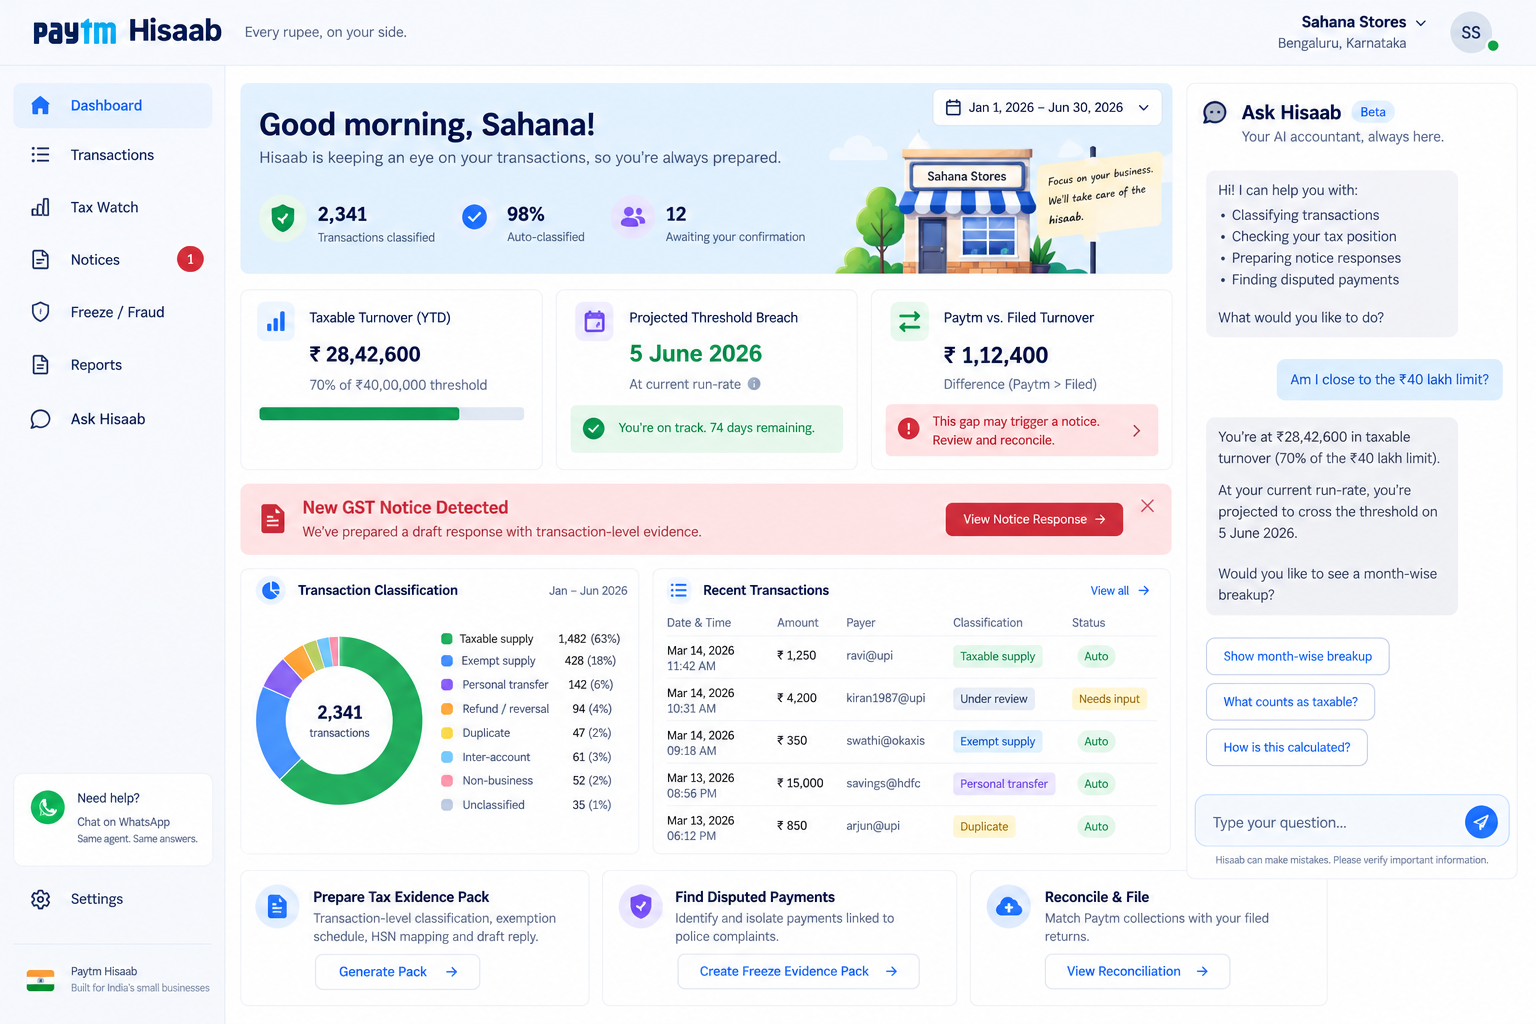
\includegraphics[width=\textwidth,height=0.70\textheight,keepaspectratio]{Paytm-Hisaab_website_look.png}
\end{center}
\vspace{0.1cm}
\hspace{0.05cm}{\scriptsize\color{muted}One surface: what every payment was classified as, how close she is to the threshold, and the packs. The same agent runs on WhatsApp, where she actually is.}
\note{{\color{navy}\bfseries\normalsize 8.~What the merchant sees}\par\vspace{0.55em}\textbf{0:20 --- a glance slide. Do not tour the UI.}
\\[0.4em]
One sentence: everything classified, how close she is to the threshold, and the
packs, on one surface.
\\[0.4em]
Then the WhatsApp point --- the same agent, where she actually is --- and advance.
\\[0.4em]
If someone asks whether this is built: the chat and the tools are live; this
screen is the product surface we are designing toward.}
\end{frame}

% ============================================================ 9. ARCHITECTURE
\begin{frame}{Built on Phinite}{Two agent graphs, four agents, ten deterministic skills}
\vspace{0.15cm}
\begin{columns}[T]
\begin{column}{0.53\textwidth}
{\scriptsize
\begin{tabular}{@{}L{1.75cm}L{4.7cm}@{}}
\multicolumn{2}{@{}l}{\color{navy}\bfseries\small hisaab-watch \;\scriptsize(autonomous: cron + API)}\\
\midrule
Provenance & proposes a tag and a reason for the hard credits \\
Evidence   & assembles packs: freeze evidence, then exemption schedules and HSN \\
\addlinespace[0.6em]
\multicolumn{2}{@{}l}{\color{navy}\bfseries\small hisaab-merchant \;\scriptsize(conversational: chat)}\\
\midrule
Merchant   & the conversation: attestation, alerts, Kannada \\
Escalation & decides when to stop and route to a human CA \\
\bottomrule
\end{tabular}}
\\[0.75em]
{\scriptsize\color{muted}The nightly pass writes its queue to the ledger; the chat reads it when she opens it. Deliberately \emph{not} a graph-to-graph call: a queue that outlives either run is what makes the handoff robust.}
\end{column}
\begin{column}{0.44\textwidth}
\card{5.7cm}{{\bfseries\color{navy}Permissions are the product}\\[0.4em]
\scriptsize Provenance proposes, \red{never commits}.\\[0.25em]
\scriptsize Merchant is the \emph{only} agent that can commit a tag.\\[0.25em]
\scriptsize Evidence is \red{read-only}. It cannot edit a classification to make a pack look better.\\[0.25em]
\scriptsize Escalation can \red{halt} any pack; a human approves.}
\\[0.5em]
\hspace{0.1cm}\begin{minipage}{5.7cm}{\scriptsize\color{muted}Ten tools run live against a hosted service. Every number in a pack traces back, in the trace, to the credit and the attestation behind it.}\end{minipage}
\end{column}
\end{columns}
\note{{\color{navy}\bfseries\normalsize 9.~Built on Phinite}\par\vspace{0.55em}\textbf{0:40 --- for the technical judges.}
\\[0.4em]
Two agent graphs, not four loose agents: \texttt{hisaab-watch} runs autonomously on
cron, \texttt{hisaab-merchant} is the conversation. The nightly pass writes a queue;
the chat reads it when she opens it --- deliberately not a graph-to-graph call,
because a queue that outlives either run is what makes the handoff robust.
\\[0.4em]
\textbf{Spend your time on the right-hand card.} The strongest line in it:
the Evidence agent is read-only --- \emph{the agent that builds the defence cannot
edit the evidence.} And only the Merchant agent can commit an attested tag.
\\[0.4em]
Those are enforced as Phinite tool policies, not conventions, and a denied call
shows up in the trace.}
\end{frame}

% ============================================================ 10. DESIGN DECISIONS
\begin{frame}{Four decisions that make it defensible}
\vspace{0.3cm}
\begin{columns}[T]
\begin{column}{0.48\textwidth}
\card{6.0cm}{{\bfseries\color{navy}1. Arithmetic lives in skills, not the model}\\[0.35em]
\scriptsize Turnover, projections and apportionment are deterministic Python: versioned, testable, traceable. Wrapping arithmetic in an LLM is the standard tell, and the trace would show it.}
\\[0.35em]
\card{6.0cm}{{\bfseries\color{navy}3. Refusing to guess is a feature}\\[0.35em]
\scriptsize An \texttt{unclassified} credit routed to the merchant costs one tap. A confident wrong tag inside an evidence pack is a catastrophe. We report the refusal rate honestly.}
\end{column}
\begin{column}{0.48\textwidth}
\card{6.0cm}{{\bfseries\color{navy}2. Attestation is the promotion boundary}\\[0.35em]
\scriptsize Nothing enters a production pack that the merchant has not confirmed. Sandbox to UAT to prod, with her tap as the gate.}
\\[0.35em]
\card{6.0cm}{{\bfseries\color{navy}4. Ground truth, so accuracy is a number}\\[0.35em]
\scriptsize We simulated a year of a shop's life from a known process, split into what Paytm can see and what really happened. Agents read only the visible half, which is why we quote error bars instead of vibes.}
\end{column}
\end{columns}
\note{{\color{navy}\bfseries\normalsize 10.~Four decisions}\par\vspace{0.55em}\textbf{0:35 --- the slide that separates you from a demo.}
\\[0.4em]
Lead with \#1: all arithmetic is deterministic Python, not model output. Wrapping
arithmetic in an LLM is the standard tell, and the trace would show it.
\\[0.4em]
Then \#3: refusing to guess is a feature. An \texttt{unclassified} credit costs one
tap; a confident wrong tag inside an evidence pack is a catastrophe.
\\[0.4em]
Skim \#2 and \#4 --- one clause each. \#4 is worth a beat if the room is technical:
we generated ground truth, so accuracy is a number instead of a claim.}
\end{frame}

% ============================================================ 11. DEMO / ATTESTATION
\begin{frame}{Demo $\cdot$ Sahana Stores, Jayanagar}{An ordinary Tuesday, before anything goes wrong}
\vspace{0.1cm}
\begin{columns}[T]
\begin{column}{0.48\textwidth}
{\scriptsize\color{muted}Tuesday 10 March. Thirty-nine credits came in over the weekend. The agent asks about \hi{three}.}
\\[0.4em]
\card{5.9cm}{{\kn\scriptsize ಭಾನುವಾರ ರಾತ್ರಿ ₹15,000. ನಿಮ್ಮ ಸ್ವಂತ ಹಣವೇ?}\\[0.25em]
{\color{muted}\scriptsize \qm{₹15,000 at 11:04pm Sunday, from your savings account. Your own money?}}\\[0.35em]
{\scriptsize\color{navy}\fbox{\kn ಹೌದು}\;\fbox{\kn ಇಲ್ಲ}}}
\\[0.4em]
{\scriptsize $\cdot$\; ₹7,500 from her husband, scanned at the shop QR\\[0.25em]
$\cdot$\; ₹4,850 from Raghu Shetty, who has bought twice before. A real sale, and the agent \emph{asks} rather than assumes.}
\\[0.4em]
{\scriptsize\color{muted}The other thirty-six settle silently, and a ₹23 payment nobody can place is left alone.}
\end{column}
\begin{column}{0.48\textwidth}
\ocard{amber}{6.1cm}{{\bfseries\color{amber}And yes, two of those three should not be there}\\[0.35em]
\scriptsize A business QR is not for personal money, and the terms say so. It arrives anyway: family, own top-ups, a chit payout. The rule does not prevent it. It only means \emph{nobody keeps a record of it.}}
\\[0.45em]
{\scriptsize Paytm already reads the signals: channel, linked VPAs, payer history. What no system has is the \hi{merchant's own answer}, given at the time, in her language, and kept.}
\\[0.45em]
{\scriptsize That record is what the next two slides are built from: first for the police, then for the department.}
\end{column}
\end{columns}
\note{{\color{navy}\bfseries\normalsize 11.~Demo --- an ordinary Tuesday (beat 1)}\par\vspace{0.55em}\textbf{0:45 --- or hand over to the live demo here.}
\\[0.4em]
Thirty-nine credits came in over the weekend, the agent asks about \textbf{three}.
Read the Kannada line if you can; otherwise read the gloss under it.
\\[0.4em]
\textbf{Do not hide from the right-hand card --- lead with it.} The mid-review
point was that personal money is not allowed on a business QR. Correct, and we say
so on the slide. The argument is that the rule does not stop it, it only means no
one records it, and an unrecorded credit is what an authority later reads as income.
\\[0.4em]
\textbf{Second half of that card matters just as much.} We are not claiming Paytm
does nothing. It already reads channel, linked VPAs and payer history. What no
system has is her own answer, captured while it is still knowable. That is the
product, and it is a smaller, truer claim than the one we started with.
\\[0.4em]
\textbf{Before going on stage:} confirm the attestation queue is whole ---
\texttt{pending\_total} must be 3. A rehearsal that taps through this beat spends the
queue, and Render needs a clear-cache redeploy to restore it.}
\end{frame}

% ============================================================ 12. DEMO / THE FREEZE
\begin{frame}{Demo $\cdot$ The emergency}{The account is frozen at 09:30 and the supplier payment is due}
\vspace{0.2cm}
\begin{columns}[T]
\begin{column}{0.46\textwidth}
{\scriptsize She sold someone 12kg of onions. That customer was three layers downstream of a fraud victim. She is not named in the FIR, which was filed in another state, and \hi{339 payments} came in that week.}
\\[0.5em]
\card{5.8cm}{{\bfseries\color{navy}The agent isolates it}\\[0.35em]
\scriptsize ₹4,200 on 21 March at 19:47, till POS01. Matched by UTR \emph{and independently} by amount and date.\\[0.3em]
\scriptsize The sale record comes with it: the POS bill, the items, the till and the minute.}
\end{column}
\begin{column}{0.49\textwidth}
\ocard{amber}{6.1cm}{{\bfseries\color{amber}And the decoy it did not choose}\\[0.35em]
\scriptsize A \emph{second} ₹4,200 that same week, from a regular customer. Listed in the pack, and explicitly \emph{not} named as the disputed one. Only the date separates them.}
\\[0.5em]
{\scriptsize Then it drafts the NCRP-CFCFRMS grievance, citing the judgments that only the \emph{disputed amount} should be lien-marked, not the whole account.}
\\[0.5em]
{\scriptsize\color{bad}\bfseries It never asserts that she is innocent.}\\[0.1em]
{\scriptsize\color{muted}Some frozen accounts genuinely are mule accounts. The agent assembles evidence; a human decides. Escalation holds the pack for approval.}
\end{column}
\end{columns}
\note{{\color{navy}\bfseries\normalsize 12.~Demo --- the emergency (beat 4)}\par\vspace{0.55em}\textbf{0:50 --- this is now the lead case. Give it the most time of the three.}
\\[0.4em]
Set the stakes in one sentence: account frozen at half nine, supplier payment due,
339 payments came in that week, and she is not named in the FIR.
\\[0.4em]
\textbf{Why this one leads.} She did nothing wrong and there is no rule she broke.
She sold onions to a customer who turned out to be laundering. Every objection
available against the tax case --- she should not have taken personal money on that
QR, she should have registered --- has no purchase here at all.
\\[0.4em]
The agent isolates ₹4,200 by UTR \emph{and independently} by amount and date, and
brings the POS bill with it --- the items, till POS01, 19:47.
\\[0.4em]
\textbf{The decoy is the point.} A second ₹4,200 that same week from a regular
customer, listed in the pack and explicitly not chosen. Anyone can match an amount;
the pack shows its work.
\\[0.4em]
Finish on the red line: it never asserts she is innocent. Some frozen accounts
genuinely are mule accounts. We assemble evidence; a human decides, and Escalation
holds the pack for approval.}
\end{frame}

% ============================================================ 13. DEMO / TAX
\begin{frame}{Demo $\cdot$ The warning, and the notice}{The same ledger, read for the other authority}
\vspace{0.15cm}
\begin{columns}[T]
\begin{column}{0.38\textwidth}
{\scriptsize\color{muted}Replayed as of 31 January:}
\\[0.35em]
\ocard{good}{4.8cm}{{\bfseries\color{ink}\scriptsize\qm{At your current rate you cross ₹40 lakh around {\color{bad}14 March}. You will need to register.}}\\[0.35em]
{\scriptsize\color{muted}\grn{43 days of warning}, and the date is computed, not typed.}}
\\[0.45em]
{\scriptsize\color{bad}\bfseries This beat is what makes the pitch safe.}\\[0.1em]
{\scriptsize\color{muted}Its first act on the tax side is telling her to register.}
\end{column}
\begin{column}{0.58\textwidth}
{\scriptsize\color{muted}Then the notice arrives, claiming {\color{bad}\bfseries ₹60.98L} of turnover:}
\\[0.3em]
{\scriptsize
\begin{tabular}{@{}lr@{\hskip 1.2em}l@{}}
\multicolumn{2}{@{}l}{\color{navy}\bfseries Aggregate turnover \quad ₹42.2L} & \sub{within \grn{1.6\%} of truth} \\
\midrule
Exempt supplies      & ₹31.3L & \sub{vegetables, loose rice} \\
Taxable supplies     & ₹10.9L & \sub{branded goods, oil, soap} \\
\addlinespace[0.45em]
\multicolumn{2}{@{}l}{\color{navy}\bfseries Not turnover at all \quad ₹18.8L} & \sub{every line traced} \\
\midrule
Her own accounts     & ₹7.4L & \sub{top-ups before supplier runs} \\
Family               & ₹6.1L & \sub{spouse, parent, in-law} \\
Loans, chit, gifts   & ₹4.3L & \sub{chit payout, festival gifts} \\
Refunds, duplicates  & ₹1.0L & \sub{crate returns, double-taps} \\
\bottomrule
\end{tabular}}
\\[0.45em]
{\scriptsize And it says plainly: \hi{the claim is wrong, and you \emph{did} cross ₹40 lakh on 14 March. You must register.}}
\end{column}
\end{columns}
\note{{\color{navy}\bfseries\normalsize 13.~Demo --- the warning and the notice (beats 2 and 3)}\par\vspace{0.55em}\textbf{0:50 --- two tax beats on one slide, deliberately compressed.}
\\[0.4em]
Left: replayed as of 31 January, the agent says she crosses ₹40 lakh around
14 March. \textbf{Say the red line out loud} --- its first act on the tax side is
telling her she owes a registration. That is what stops the room turning hostile.
\\[0.4em]
Right: the notice claims ₹60.98 lakh, and the pack answers it line by line, every
figure traceable to transaction IDs. Then the honest half:
\textbf{the claim is wrong, and she did cross ₹40 lakh, and she must register.}
\\[0.4em]
\textbf{If a judge diffs this against slide 5:} slide 5 shows seeded truth
(₹42.9L), this shows what our system computed (₹42.2L). The 1.6\% between them
\emph{is} the accuracy claim --- say that, do not hedge.
\\[0.4em]
\textbf{If pushed on the personal and own-account lines:} same answer as slide 11.
Those credits should not be on a business QR, they are there anyway, and the
alternative to classifying them is letting them be read as income.}
\end{frame}

% ============================================================ 14. NUMBERS
\begin{frame}{What we can actually prove}{One merchant, one year, 13,267 credits, scored against seeded truth}
\vspace{0.45cm}
\begin{columns}[T]
\begin{column}{0.33\textwidth}
\begin{center}\bignum{1.6\%}{error on aggregate turnover\\ (taxable share within 1\%)}\end{center}
\vspace{0.55cm}
\begin{center}\bignum{43 days}{of warning before the\\ threshold crossing}\end{center}
\end{column}
\begin{column}{0.33\textwidth}
\begin{center}\bignum{1.3 a day}{median questions asked.\\ 189 in a year, never over 3}\end{center}
\vspace{0.55cm}
\begin{center}\bignum{zero}{credits left untagged\\ across the whole year}\end{center}
\end{column}
\begin{column}{0.30\textwidth}
\card{3.8cm}{{\bfseries\color{navy}The honest baseline}\\[0.35em]
\scriptsize A 50-line rules-only classifier gets 99.3\% on sale vs not-a-sale, but catches only \red{77.8\%} of non-sale credits.\\[0.3em]
\scriptsize That residue alone puts two eval merchants on the \emph{wrong side} of ₹40L.\\[0.3em]
\scriptsize Closing it is what the agent plus one tap is for.}
\end{column}
\end{columns}
\vspace{0.45cm}
\hspace{0.1cm}{\scriptsize\color{muted}She corrected the agent 52 times that year. Those corrections are the ledger's strongest evidence, not its failures.}
\note{{\color{navy}\bfseries\normalsize 14.~What we can actually prove}\par\vspace{0.55em}\textbf{0:30 --- do not read all four. Pick two.}
\\[0.4em]
Lead with \textbf{1.6\%} error on turnover and \textbf{1.3 questions a day}. The
other two are there to be read, not narrated.
\\[0.4em]
\textbf{The credibility move is the box on the right} --- volunteer the weakness
before anyone finds it. A rules-only baseline gets 99.3\% on sale vs not-a-sale
but catches only 77.8\% of non-sale credits, and that residue alone puts two eval
merchants on the wrong side of ₹40 lakh. Closing it is what the agent plus one tap is for.
\\[0.4em]
Last line if you have the beat: she corrected the agent 52 times that year, and
those corrections are the ledger's strongest evidence, not its failures.}
\end{frame}

% ============================================================ 15. CLOSE
\begin{frame}{The line we do not cross}{Accuracy, not minimisation}
\vspace{0.3cm}
\begin{columns}[T]
\begin{column}{0.52\textwidth}
{\scriptsize
$\cdot$\; We \hi{never assert innocence} on a freeze. Some accounts really are mule accounts. We assemble evidence; a human decides.\\[0.5em]
$\cdot$\; We \hi{file nothing} with any authority. Artefacts only; the merchant or their CA files.\\[0.5em]
$\cdot$\; We compute what she \hi{genuinely owes} and say so plainly, including \qm{you crossed the threshold, you must register.}\\[0.5em]
$\cdot$\; We \hi{never assert a final liability}. We compute, show the workings, and route to a CA.\\[0.5em]
$\cdot$\; A business QR is \hi{not for personal money}. We do not excuse it. We record it, so it is not read as income.}
\end{column}
\begin{column}{0.44\textwidth}
\begin{tikzpicture}\node[rounded corners=4pt,fill=navy,text=white,inner sep=10pt,text width=5.7cm,align=left]{
{\bfseries Why this has to be Paytm}\\[0.45em]
\scriptsize The rail is the only place provenance is cheap. Everyone else arrives eighteen months late, when the answer is already unrecoverable.\\[0.45em]
\scriptsize A frozen merchant cannot transact at all: dead Soundbox and zero GMV the same morning, before it becomes the sign on the shutter, \emph{\qm{No UPI. Cash only.}}
};\end{tikzpicture}
\end{column}
\end{columns}
\vspace{0.4cm}
\begin{center}
{\large\color{navy}\bfseries Paytm Hisaab}\quad{\color{muted}every rupee, on your side.}
\end{center}
\note{{\color{navy}\bfseries\normalsize 15.~The line we do not cross}\par\vspace{0.55em}\textbf{0:30 --- the non-negotiables, fast, then land.}
\\[0.4em]
Run the five bullets at pace. The one to hit is the first: we never assert
innocence on a freeze. The last is the mid-review answer, on the slide on purpose.
\\[0.4em]
Then the navy box: provenance is cheap only on the rail, and a frozen merchant
stops transacting the same morning.
\\[0.4em]
Final line, unhurried: \emph{``Paytm Hisaab. Every rupee, on your side.''} Stop talking.
\\[0.5em]
{\scriptsize
{\color{navy}\bfseries --- Q\&A prep ---}
\\[0.3em]
\textbf{``Merchants may not take personal money on a business QR.''} Correct, and
slide 11 says so before you have to. It arrives anyway, and the alternative to
recording it is letting an authority read it as income. We are not defending the
behaviour --- we are refusing to let it become a liability.
\\[0.3em]
\textbf{``Paytm already tags transactions.''} It does, and we build on that rather
than around it: channel, linked VPAs and payer history feed the rules layer. What
no tag carries is her attestation --- the part an authority accepts, and the only
part she alone can give.
\\[0.3em]
\textbf{``No return mismatch?''} That check needs a \emph{registered} composition
dealer who filed a CMP-08 to disagree with. Ours is unregistered, which is why she
gets a notice at all; the eval split has one with four quarters seeded.
\\[0.3em]
\textbf{``Exempt vs taxable on a QR sale?''} Not per payment. We apportion by value
from that shop's own POS-billed ratio and label it an estimate. Labelling each sale
by its majority side understated taxable turnover threefold.
\\[0.3em]
\textbf{``Four LLM calls in a trenchcoat?''} Everything deterministic is a skill and
four agents is the ceiling. If twenty lines of Python replaces an agent, it should
have been a skill --- the trace shows which is which.
\\[0.3em]
\textbf{``No standing with the police.''} Agreed: Paytm supplies, the merchant
files. By design. Cash sales are real, out of scope, and on the slide.}}
\end{frame}

\end{document}
"
\ifdefined\shownotes
  \setbeamertemplate{note page}{%
    \usebeamercolor[fg]{normal text}%
    \vspace{0.2em}%
    {\scriptsize\color{muted}Paytm Hisaab \;$\cdot$\; speaker notes}\hfill
    {\scriptsize\color{muted}slide \insertframenumber\ of 15}\par
    \vspace{0.25em}{\color{ptmcyan}\rule{\textwidth}{1.5pt}}\par
    \vspace{0.55em}\footnotesize\raggedright\insertnote\par}
  \setbeameroption{show only notes}
\fi

\begin{document}

% ============================================================ 1. TITLE
{\setbeamertemplate{footline}{}
\begin{frame}[plain]
\vspace{0.9cm}
\begin{center}
{\fontsize{38}{42}\selectfont\bfseries\color{navy}Paytm\;\color{ink}Hisaab}\\[0.45em]
{\Large\color{muted}Every rupee, on your side.}\\[0.9em]
{\color{ptmcyan}\rule{2.8cm}{2.5pt}}\\[0.9em]
{\large\color{ink}The agent that lets a merchant account for their own money}\\[0.15em]
{\large\color{ink}when someone in authority demands an explanation.}\\[1.3em]
{\small\color{muted}Agent Labs Buildathon \;$\cdot$\; Phinite $\times$ Paytm \;$\cdot$\; Track 2: AI for Small Businesses}
\end{center}
\note{{\color{navy}\bfseries\normalsize 1.~Title}\par\vspace{0.55em}\textbf{0:10 --- open cold.} Do not read the title or the tagline off the slide.
\\[0.4em]
Say: \emph{``I want to tell you about a man in Haveri who opened an envelope.''} Then advance.
\\[0.4em]
Nothing on this slide needs explaining. The tagline lands at the end, not here.}
\end{frame}}

% ============================================================ 2. STORY
\begin{frame}{Haveri, 2025}{A vegetable vendor opens an envelope}
\vspace{0.05cm}
\begin{columns}[T]
\begin{column}{0.52\textwidth}
\vspace{0.15cm}
He sells vegetables. Vegetables are \hi{exempt} from GST.\\[0.6em]
He also took UPI, because Paytm asked him to.\\[0.6em]
Four years of credits into his account, added up and billed as income:
\begin{center}\vspace{0.1em}{\fontsize{30}{32}\selectfont\bfseries\color{bad}₹29 lakh}\end{center}
\end{column}
\begin{column}{0.44\textwidth}
\ocard{hairline}{5.4cm}{\centering
  {\color{muted}\scriptsize Within weeks, on shutters across Karnataka:}\\[0.6em]
  {\fontsize{20}{23}\selectfont\bfseries\color{ink}\qm{No UPI.\\ Cash only.}}\\[0.6em]
  {\color{muted}\scriptsize A statewide boycott, by the merchants who had just adopted it.}}
\end{column}
\end{columns}
\vspace{0.25cm}
\hspace{0.1cm}{\small\sub{Withdrawn for the traders who could \emph{show} what they sold. Most could not. And tax is no longer the only authority asking.}}
\note{{\color{navy}\bfseries\normalsize 2.~Haveri, 2025}\par\vspace{0.55em}\textbf{0:45 --- the hook. Tell it, do not summarise it.}
\\[0.4em]
Four beats, in this order: he sells vegetables; vegetables are exempt from GST;
he took UPI because \emph{we} asked him to; the department added up four years of
credits and sent him a bill for \textbf{₹29 lakh}.
\\[0.4em]
\textbf{Pause on the number.} Then the card: within weeks, shutters across Karnataka
read ``No UPI, cash only.'' Merchants we had just onboarded, boycotting the rail.
\\[0.4em]
Close on the bottom line --- the notices were withdrawn for traders who could
\emph{show} what they sold. Most could not. That verb is the whole product.
\\[0.4em]
\textbf{Then the bridge:} \emph{``and tax is no longer the only authority asking.''}
That sentence is doing the repositioning --- Haveri is not a tax story here, it is
the moment taking digital money became a liability. The sharper version of it is
two slides away.
\\[0.4em]
\textbf{Do not say this is happening right now.} It is 2025. The next slide is
what makes it current, and a judge who knows the episode will respect the distinction.}
\end{frame}

% ============================================================ 3. STILL HAPPENING
\begin{frame}{And this is not a 2025 story}{CAclubindia, last updated 02 September 2026: ten days ago}
\vspace{0.1cm}
\begin{center}

\includegraphics[width=12.4cm]{gst-notices-2026.png}
\end{center}
\vspace{0.35cm}
\card{13.1cm}{\scriptsize\qm{During August 2026, the GST Department issued a significant number of notices covering different financial years and involving a wide range of issues\ldots\ They covered matters such as ITC mismatches, ineligible credit, \hi{differences in turnover}, wrong GST classification or rate, \hi{exemption claims}, Reverse Charge Mechanism\ldots}}
\vspace{0.3cm}

\hspace{0.1cm}{\small Those two categories are the whole content of an evidence pack. And this is the \emph{slower} of the two authorities. The other one freezes the account first.}
\note{{\color{navy}\bfseries\normalsize 3.~And this is not a 2025 story}\par\vspace{0.55em}\textbf{0:25 --- fast. This slide exists to kill one objection.}
\\[0.4em]
Say: \emph{``That was last year. This was published ten days ago.''}
\\[0.4em]
Do not read the quote. Point at the two bolded phrases only ---
\textbf{differences in turnover} and \textbf{exemption claims} --- and say those
two categories are the entire content of what we build.
\\[0.4em]
\textbf{Land on the last line and move.} It is the handoff into the police
slide: this is the slower authority. The other one freezes first and asks
afterwards. Do not linger here --- tax is no longer the headline.}
\end{frame}

% ============================================================ 4. THE TRAP
\begin{frame}{Every rupee a merchant receives is now evidence}{Today it is only ever used against them}
\vspace{0.05cm}
\begin{columns}[T]
\begin{column}{0.47\textwidth}
\ocard{bad}{6.0cm}{{\bfseries\color{bad}The cyber-crime police}\\[0.35em]
\scriptsize Fraud money layers through accounts within minutes. The shop at the end of the chain, the one that sold someone a watermelon, is frozen. It did nothing wrong, is not named in the FIR, and finds out when a payment declines.}
\end{column}
\begin{column}{0.47\textwidth}
\card{6.1cm}{{\bfseries\color{navy}The tax department}\\[0.35em]
\scriptsize Compares UPI collections against filed returns and bills the difference. Registered traders too, with QR, wallet, card and cash deposits all in scope.}
\end{column}
\end{columns}
\vspace{0.4cm}
\begin{center}
{\large Both demand the same artefact: \hi{what was each rupee, actually?}}\\[0.3em]
{\small\color{muted}Paytm already sees more of this than anyone. What is missing is the \emph{merchant's own answer}, captured when it is still knowable.}
\end{center}
\vspace{0.15cm}
{\color{hairline}\hrule height 1pt}
\vspace{0.35em}
\hspace{0.05cm}{\scriptsize\bfseries\color{bad}What it costs Paytm:}~{\scriptsize a frozen merchant stops transacting that morning. A frightened one takes the QR down for good. Dead Soundbox, zero GMV, no lending origination.}
\note{{\color{navy}\bfseries\normalsize 4.~Every rupee is now evidence}\par\vspace{0.55em}\textbf{0:40 --- two authorities, one unanswerable question.}
\\[0.4em]
\textbf{Left card first and give it the time.} Fraud money layers within minutes,
and the shop at the end of the chain, \emph{the one that sold someone a watermelon},
gets frozen. It did nothing wrong, it is not named in the FIR, and it finds out
when a payment declines. Use the watermelon.
\\[0.4em]
Right card briskly: the department reconciles collections against filed returns
and bills the difference. One sentence, then move.
\\[0.4em]
Then the pivot: both demand the same artefact --- what was each rupee, actually.
\\[0.4em]
\textbf{Say the grey line as written.} We do \emph{not} claim Paytm does nothing
with this data --- it tags plenty. The gap is the merchant's own answer, captured
when it is still knowable. Claiming otherwise in this room gets corrected.
\\[0.4em]
\textbf{Slow down for the red line.} This is the business case, not a footnote:
a frozen merchant stops transacting that morning, a frightened one takes the QR
down for good. Dead Soundbox, zero GMV, no lending origination.}
\end{frame}

% ============================================================ 5. THE BAR
\begin{frame}{Gross credits are not turnover}{One shop, one year, ₹60.98 lakh of credits}
\vspace{0.1cm}
\begin{center}
\begin{tikzpicture}[x=1cm,y=1cm]
% --- what the notice counts
\node[anchor=west,font=\scriptsize\bfseries,text=bad] at (-0.05,1.80) {WHAT THE NOTICE COUNTS AS TURNOVER};
\fill[bad!85,rounded corners=2pt] (0,1.06) rectangle (11.4,1.60);
\node[font=\small\bfseries,text=white] at (5.7,1.33) {₹60.98 lakh};

% --- what actually happened   (1 lakh = 0.18696 cm, so the bars are the same length)
\node[anchor=west,font=\scriptsize\bfseries,text=navy] at (-0.05,0.66) {WHAT ACTUALLY HAPPENED};
\fill[good!80,rounded corners=2pt]  (0,-0.08)     rectangle (6.001,0.46);
\fill[good!45]                      (6.001,-0.08) rectangle (8.002,0.46);
\fill[ptmcyan!70]                   (8.002,-0.08) rectangle (9.385,0.46);
\fill[navy!55]                      (9.385,-0.08) rectangle (10.451,0.46);
\fill[amber!70]                     (10.451,-0.08)rectangle (11.255,0.46);
\fill[muted!60,rounded corners=2pt] (11.255,-0.08)rectangle (11.4,0.46);

% brackets
\draw[navy,line width=0.8pt] (0,-0.22) -- (0,-0.36) -- (8.002,-0.36) -- (8.002,-0.22);
\node[anchor=north,font=\scriptsize,text=navy,align=center] at (4.0,-0.38)
  {\bfseries ₹42.9L aggregate turnover\quad{\color{muted}\scriptsize exempt ₹32.1L + taxable ₹10.7L}};
\draw[bad,line width=0.8pt] (8.002,-0.22) -- (8.002,-0.36) -- (11.4,-0.36) -- (11.4,-0.22);
\node[anchor=north,font=\scriptsize,text=bad,align=center] at (9.7,-0.38)
  {\bfseries ₹18.1L that is not turnover at all};

% legend
\node[font=\scriptsize,text=ink] at (5.7,-1.02) {%
\textcolor{good!80}{$\blacksquare$}~Exempt sales \quad
\textcolor{good!45}{$\blacksquare$}~Taxable sales \quad
\textcolor{ptmcyan!70}{$\blacksquare$}~Her own accounts ₹7.4L};
\node[font=\scriptsize,text=ink] at (5.7,-1.40) {%
\textcolor{navy!55}{$\blacksquare$}~Family ₹5.7L \quad
\textcolor{amber!70}{$\blacksquare$}~Loans, chit, gifts ₹4.3L \quad
\textcolor{muted!60}{$\blacksquare$}~Refunds \& duplicates ₹0.7L};
\end{tikzpicture}
\end{center}
\vspace{0.15cm}
\hspace{0.1cm}{\small\sub{Personal money does not belong on a business QR. It arrives anyway, reads as turnover, and hides the one credit the police will ask about.}}
\note{{\color{navy}\bfseries\normalsize 5.~Gross credits are not turnover}\par\vspace{0.55em}\textbf{0:45 --- the hinge of the pitch. Let the picture work.}
\\[0.4em]
Say: \emph{``One shop, one year, ₹60.98 lakh of credits. The red bar is what the
notice counts as turnover --- all of it.''}
\\[0.4em]
Then the bottom bar. \textbf{Stop talking for two seconds} and let them read it.
\\[0.4em]
₹42.9L really is turnover, and we say so. ₹18.1L is not: her savings account, her
husband, a chit payout, a double-tap on the Soundbox.
\\[0.4em]
\textbf{Get in front of the obvious objection.} Personal money is not supposed to
touch a business QR. Say so first, then say it arrives anyway --- that is an
observation about merchants, not a loophole we are selling. The rule does not stop
it; it only means no one is keeping a record of it.
\\[0.4em]
\textbf{And close on the second use.} This volume is also why she cannot find the
one credit the police care about. Same bar, same problem, and the freeze slide
pays it off.
\\[0.4em]
If challenged on the numbers: seeded ground truth from our generator, not an
estimate. Accuracy against it is slide 14.}
\end{frame}

% ============================================================ 6. INSIGHT
\begin{frame}{The insight}{Most teams would build the tax tool \emph{or} the fraud tool. They are the same engine.}
\vspace{0.15cm}
\begin{center}
\begin{tikzpicture}[font=\scriptsize]
\node[rounded corners=4pt,fill=navy,text=white,inner sep=7pt,align=center,text width=3.5cm]
  (eng) {\bfseries\small Provenance Ledger\\[0.15em] a merchant-attested label on every incoming credit};
\node[rounded corners=4pt,fill=tint,draw=bad,inner sep=6pt,align=center,text width=4.0cm]
  (tax) at ($(eng.east)+(3.7,0.78)$) {\bfseries The disputed rupee\\ freeze pack, NCRP grievance};
\node[rounded corners=4pt,fill=tint,draw=hairline,inner sep=6pt,align=center,text width=4.0cm]
  (fra) at ($(eng.east)+(3.7,-0.78)$) {\bfseries Defensible turnover\\ threshold watch, notice pack};
\draw[-{Stealth[length=2.5mm]},ptmcyan,line width=1.3pt] (eng.east) -- ++(0.5,0) |- (tax.west);
\draw[-{Stealth[length=2.5mm]},ptmcyan,line width=1.3pt] (eng.east) -- ++(0.5,0) |- (fra.west);
\node[anchor=east,text width=2.9cm,align=right,text=muted] at ($(eng.west)+(-0.35,0)$)
  {Both are downstream \emph{reads} of one ledger. Two output formats, not two products.};
\end{tikzpicture}
\end{center}
\vspace{0.1cm}
\begin{center}
\begin{tikzpicture}\node[rounded corners=4pt,fill=tint,inner sep=8pt,text width=11.2cm,align=center]{
{\bfseries\color{navy}The wedge nobody else has.}\\[0.25em]
\small Khatabook and Vyapar keep books after the fact. ClearTax files after the fact.\\
Neither sits on the rail \emph{at the moment money moves}. Paytm does.\\[0.25em]
\small Classification is cheap at the instant of the transaction,\\ and unrecoverable eighteen months later.
};\end{tikzpicture}
\end{center}
\note{{\color{navy}\bfseries\normalsize 6.~The insight}\par\vspace{0.55em}\textbf{0:40 --- why this is one product, not two.}
\\[0.4em]
Say: \emph{``Most teams would build the fraud tool or the tax tool. They are the
same engine.''} Both are downstream reads of one ledger --- two output formats,
and the freeze pack is the one we lead with.
\\[0.4em]
Then the wedge, and say it slowly because it is the defensible-moat answer:
Khatabook and Vyapar keep books after the fact, ClearTax files after the fact.
Neither sits on the rail at the moment money moves. \textbf{Paytm does.}
\\[0.4em]
Landing line: classification is cheap and accurate at the instant of the
transaction, and unrecoverable eighteen months later when the notice arrives.}
\end{frame}

% ============================================================ 7. THE ENGINE
\begin{frame}{The engine}{Eight tags, one tap}
\vspace{0.15cm}
\begin{columns}[T]
\begin{column}{0.45\textwidth}
{\color{navy}\bfseries\small Every incoming credit gets one tag}\\[0.4em]
{\scriptsize
\begin{tabular}{@{}ll@{}}
\texttt{taxable\_supply}    & ordinary sale \\
\texttt{exempt\_supply}     & vegetables, milk, loose rice \\
\texttt{personal\_transfer} & spouse, parent, sibling \\
\texttt{inter\_account}     & her own money \\
\texttt{refund\_reversal}   & money back from a vendor \\
\texttt{duplicate}          & paid twice, one refunded \\
\texttt{non\_business}      & loan, chit payout, gift \\
{\color{bad}\texttt{unclassified}} & {\color{bad}not enough signal: ask her} \\
\end{tabular}}
\\[0.75em]
{\scriptsize\color{muted}98.6\% are ordinary sales, settled by rules. The agent reasons only about the 1.4\% that need judgement.}
\end{column}
\begin{column}{0.51\textwidth}
\card{6.6cm}{{\bfseries\color{navy}The agent proposes. The merchant attests.}\\[0.4em]
\scriptsize You cannot infer \qm{my husband sent this} from a QR payment. The agent proposes a tag \emph{with its reason}; she confirms with one tap, in Kannada, batched daily.\\[0.45em]
\scriptsize Not a fallback. A ledger she attested \emph{at the time} survives a hearing. An algorithm's guess, made under duress a year later, does not.}
\\[0.55em]
\hspace{0.15cm}\begin{minipage}{6.6cm}
{\bfseries\color{navy}\small Budget: at most 3 questions a day.}\\[0.15em]
{\scriptsize\color{muted}Over a simulated year: \hi{189 questions, median 1.3 a day}. Ask more and the product is dead.}
\end{minipage}
\end{column}
\end{columns}
\note{{\color{navy}\bfseries\normalsize 7.~The engine}\par\vspace{0.55em}\textbf{0:45 --- the mechanism. Do not read the tag list.}
\\[0.4em]
Gesture at the eight tags, say ``eight labels, every incoming credit gets one,''
and move to the right-hand card, which is the real content.
\\[0.4em]
\textbf{The line that matters:} you cannot infer ``my husband sent this'' from a
QR payment. So the agent proposes a tag \emph{with its reason} and she confirms
with one tap. This is not a fallback --- a ledger she attested contemporaneously
survives a hearing; an algorithm's guess produced under duress a year later does not.
\\[0.4em]
Then the budget: at most three questions a day, and we measured 189 across a
year, median 1.3. Ask more than that and the product is dead.
\\[0.4em]
If asked about cost: 98.6\% are ordinary sales settled by rules. The model only
sees the 1.4\% that need judgement.}
\end{frame}

% ============================================================ 8. PRODUCT
\begin{frame}{What the merchant sees}
\vspace{-0.1cm}
\begin{center}
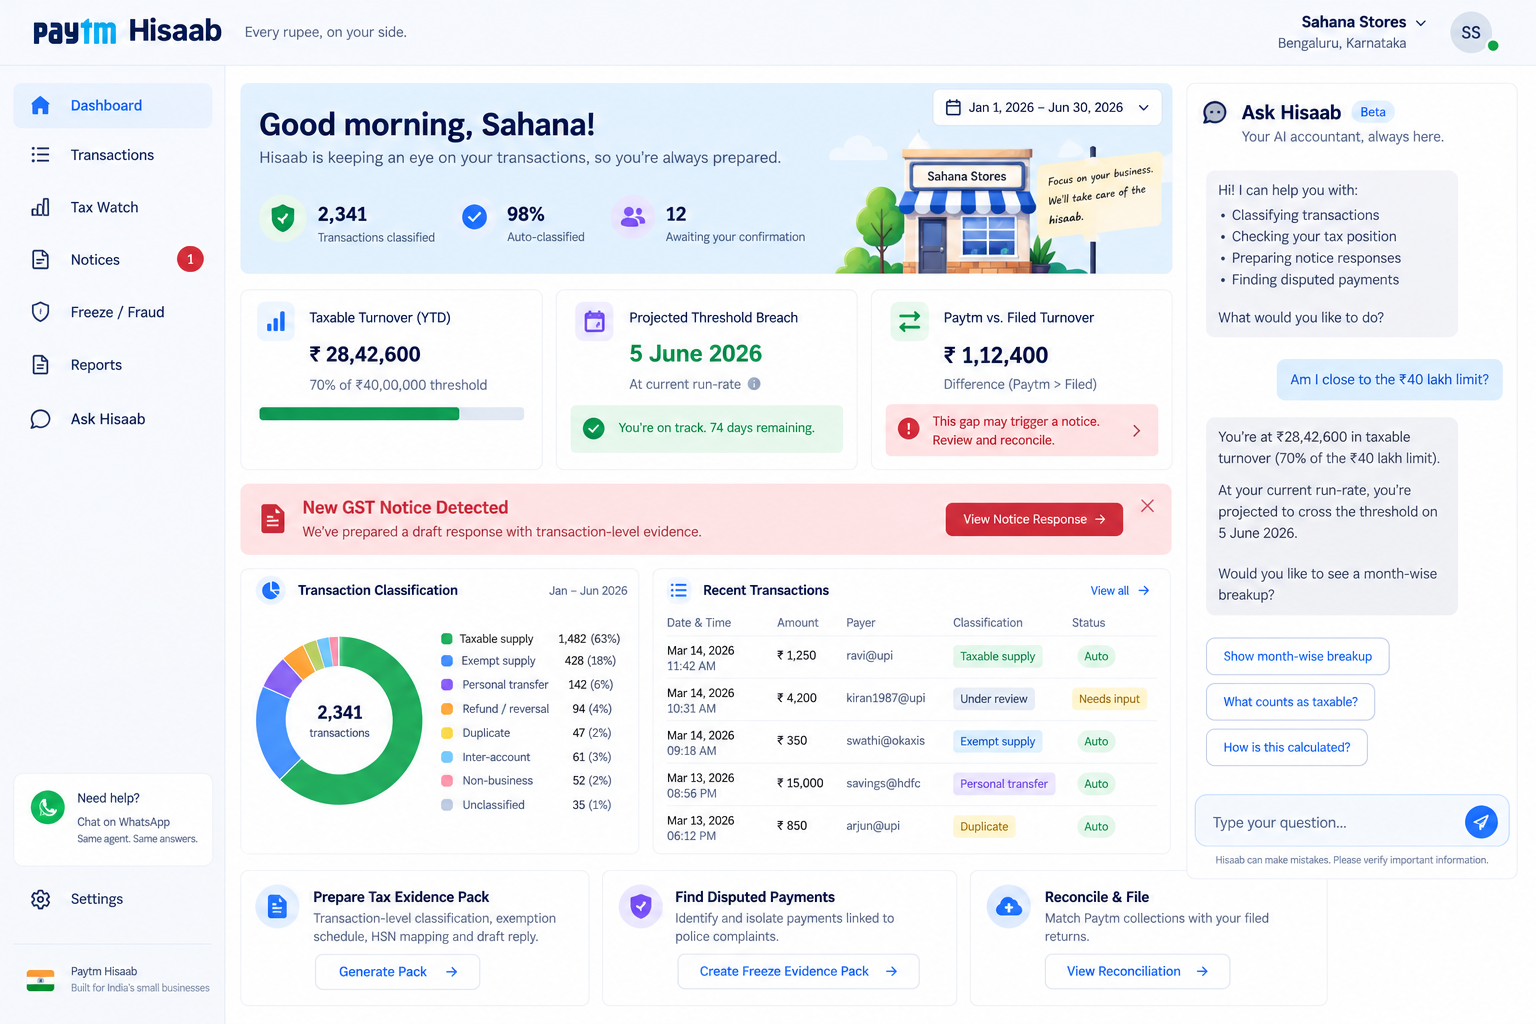
\includegraphics[width=\textwidth,height=0.70\textheight,keepaspectratio]{Paytm-Hisaab_website_look.png}
\end{center}
\vspace{0.1cm}
\hspace{0.05cm}{\scriptsize\color{muted}One surface: what every payment was classified as, how close she is to the threshold, and the packs. The same agent runs on WhatsApp, where she actually is.}
\note{{\color{navy}\bfseries\normalsize 8.~What the merchant sees}\par\vspace{0.55em}\textbf{0:20 --- a glance slide. Do not tour the UI.}
\\[0.4em]
One sentence: everything classified, how close she is to the threshold, and the
packs, on one surface.
\\[0.4em]
Then the WhatsApp point --- the same agent, where she actually is --- and advance.
\\[0.4em]
If someone asks whether this is built: the chat and the tools are live; this
screen is the product surface we are designing toward.}
\end{frame}

% ============================================================ 9. ARCHITECTURE
\begin{frame}{Built on Phinite}{Two agent graphs, four agents, ten deterministic skills}
\vspace{0.15cm}
\begin{columns}[T]
\begin{column}{0.53\textwidth}
{\scriptsize
\begin{tabular}{@{}L{1.75cm}L{4.7cm}@{}}
\multicolumn{2}{@{}l}{\color{navy}\bfseries\small hisaab-watch \;\scriptsize(autonomous: cron + API)}\\
\midrule
Provenance & proposes a tag and a reason for the hard credits \\
Evidence   & assembles packs: freeze evidence, then exemption schedules and HSN \\
\addlinespace[0.6em]
\multicolumn{2}{@{}l}{\color{navy}\bfseries\small hisaab-merchant \;\scriptsize(conversational: chat)}\\
\midrule
Merchant   & the conversation: attestation, alerts, Kannada \\
Escalation & decides when to stop and route to a human CA \\
\bottomrule
\end{tabular}}
\\[0.75em]
{\scriptsize\color{muted}The nightly pass writes its queue to the ledger; the chat reads it when she opens it. Deliberately \emph{not} a graph-to-graph call: a queue that outlives either run is what makes the handoff robust.}
\end{column}
\begin{column}{0.44\textwidth}
\card{5.7cm}{{\bfseries\color{navy}Permissions are the product}\\[0.4em]
\scriptsize Provenance proposes, \red{never commits}.\\[0.25em]
\scriptsize Merchant is the \emph{only} agent that can commit a tag.\\[0.25em]
\scriptsize Evidence is \red{read-only}. It cannot edit a classification to make a pack look better.\\[0.25em]
\scriptsize Escalation can \red{halt} any pack; a human approves.}
\\[0.5em]
\hspace{0.1cm}\begin{minipage}{5.7cm}{\scriptsize\color{muted}Ten tools run live against a hosted service. Every number in a pack traces back, in the trace, to the credit and the attestation behind it.}\end{minipage}
\end{column}
\end{columns}
\note{{\color{navy}\bfseries\normalsize 9.~Built on Phinite}\par\vspace{0.55em}\textbf{0:40 --- for the technical judges.}
\\[0.4em]
Two agent graphs, not four loose agents: \texttt{hisaab-watch} runs autonomously on
cron, \texttt{hisaab-merchant} is the conversation. The nightly pass writes a queue;
the chat reads it when she opens it --- deliberately not a graph-to-graph call,
because a queue that outlives either run is what makes the handoff robust.
\\[0.4em]
\textbf{Spend your time on the right-hand card.} The strongest line in it:
the Evidence agent is read-only --- \emph{the agent that builds the defence cannot
edit the evidence.} And only the Merchant agent can commit an attested tag.
\\[0.4em]
Those are enforced as Phinite tool policies, not conventions, and a denied call
shows up in the trace.}
\end{frame}

% ============================================================ 10. DESIGN DECISIONS
\begin{frame}{Four decisions that make it defensible}
\vspace{0.3cm}
\begin{columns}[T]
\begin{column}{0.48\textwidth}
\card{6.0cm}{{\bfseries\color{navy}1. Arithmetic lives in skills, not the model}\\[0.35em]
\scriptsize Turnover, projections and apportionment are deterministic Python: versioned, testable, traceable. Wrapping arithmetic in an LLM is the standard tell, and the trace would show it.}
\\[0.35em]
\card{6.0cm}{{\bfseries\color{navy}3. Refusing to guess is a feature}\\[0.35em]
\scriptsize An \texttt{unclassified} credit routed to the merchant costs one tap. A confident wrong tag inside an evidence pack is a catastrophe. We report the refusal rate honestly.}
\end{column}
\begin{column}{0.48\textwidth}
\card{6.0cm}{{\bfseries\color{navy}2. Attestation is the promotion boundary}\\[0.35em]
\scriptsize Nothing enters a production pack that the merchant has not confirmed. Sandbox to UAT to prod, with her tap as the gate.}
\\[0.35em]
\card{6.0cm}{{\bfseries\color{navy}4. Ground truth, so accuracy is a number}\\[0.35em]
\scriptsize We simulated a year of a shop's life from a known process, split into what Paytm can see and what really happened. Agents read only the visible half, which is why we quote error bars instead of vibes.}
\end{column}
\end{columns}
\note{{\color{navy}\bfseries\normalsize 10.~Four decisions}\par\vspace{0.55em}\textbf{0:35 --- the slide that separates you from a demo.}
\\[0.4em]
Lead with \#1: all arithmetic is deterministic Python, not model output. Wrapping
arithmetic in an LLM is the standard tell, and the trace would show it.
\\[0.4em]
Then \#3: refusing to guess is a feature. An \texttt{unclassified} credit costs one
tap; a confident wrong tag inside an evidence pack is a catastrophe.
\\[0.4em]
Skim \#2 and \#4 --- one clause each. \#4 is worth a beat if the room is technical:
we generated ground truth, so accuracy is a number instead of a claim.}
\end{frame}

% ============================================================ 11. DEMO / ATTESTATION
\begin{frame}{Demo $\cdot$ Sahana Stores, Jayanagar}{An ordinary Tuesday, before anything goes wrong}
\vspace{0.1cm}
\begin{columns}[T]
\begin{column}{0.48\textwidth}
{\scriptsize\color{muted}Tuesday 10 March. Thirty-nine credits came in over the weekend. The agent asks about \hi{three}.}
\\[0.4em]
\card{5.9cm}{{\kn\scriptsize ಭಾನುವಾರ ರಾತ್ರಿ ₹15,000. ನಿಮ್ಮ ಸ್ವಂತ ಹಣವೇ?}\\[0.25em]
{\color{muted}\scriptsize \qm{₹15,000 at 11:04pm Sunday, from your savings account. Your own money?}}\\[0.35em]
{\scriptsize\color{navy}\fbox{\kn ಹೌದು}\;\fbox{\kn ಇಲ್ಲ}}}
\\[0.4em]
{\scriptsize $\cdot$\; ₹7,500 from her husband, scanned at the shop QR\\[0.25em]
$\cdot$\; ₹4,850 from Raghu Shetty, who has bought twice before. A real sale, and the agent \emph{asks} rather than assumes.}
\\[0.4em]
{\scriptsize\color{muted}The other thirty-six settle silently, and a ₹23 payment nobody can place is left alone.}
\end{column}
\begin{column}{0.48\textwidth}
\ocard{amber}{6.1cm}{{\bfseries\color{amber}And yes, two of those three should not be there}\\[0.35em]
\scriptsize A business QR is not for personal money, and the terms say so. It arrives anyway: family, own top-ups, a chit payout. The rule does not prevent it. It only means \emph{nobody keeps a record of it.}}
\\[0.45em]
{\scriptsize Paytm already reads the signals: channel, linked VPAs, payer history. What no system has is the \hi{merchant's own answer}, given at the time, in her language, and kept.}
\\[0.45em]
{\scriptsize That record is what the next two slides are built from: first for the police, then for the department.}
\end{column}
\end{columns}
\note{{\color{navy}\bfseries\normalsize 11.~Demo --- an ordinary Tuesday (beat 1)}\par\vspace{0.55em}\textbf{0:45 --- or hand over to the live demo here.}
\\[0.4em]
Thirty-nine credits came in over the weekend, the agent asks about \textbf{three}.
Read the Kannada line if you can; otherwise read the gloss under it.
\\[0.4em]
\textbf{Do not hide from the right-hand card --- lead with it.} The mid-review
point was that personal money is not allowed on a business QR. Correct, and we say
so on the slide. The argument is that the rule does not stop it, it only means no
one records it, and an unrecorded credit is what an authority later reads as income.
\\[0.4em]
\textbf{Second half of that card matters just as much.} We are not claiming Paytm
does nothing. It already reads channel, linked VPAs and payer history. What no
system has is her own answer, captured while it is still knowable. That is the
product, and it is a smaller, truer claim than the one we started with.
\\[0.4em]
\textbf{Before going on stage:} confirm the attestation queue is whole ---
\texttt{pending\_total} must be 3. A rehearsal that taps through this beat spends the
queue, and Render needs a clear-cache redeploy to restore it.}
\end{frame}

% ============================================================ 12. DEMO / THE FREEZE
\begin{frame}{Demo $\cdot$ The emergency}{The account is frozen at 09:30 and the supplier payment is due}
\vspace{0.2cm}
\begin{columns}[T]
\begin{column}{0.46\textwidth}
{\scriptsize She sold someone 12kg of onions. That customer was three layers downstream of a fraud victim. She is not named in the FIR, which was filed in another state, and \hi{339 payments} came in that week.}
\\[0.5em]
\card{5.8cm}{{\bfseries\color{navy}The agent isolates it}\\[0.35em]
\scriptsize ₹4,200 on 21 March at 19:47, till POS01. Matched by UTR \emph{and independently} by amount and date.\\[0.3em]
\scriptsize The sale record comes with it: the POS bill, the items, the till and the minute.}
\end{column}
\begin{column}{0.49\textwidth}
\ocard{amber}{6.1cm}{{\bfseries\color{amber}And the decoy it did not choose}\\[0.35em]
\scriptsize A \emph{second} ₹4,200 that same week, from a regular customer. Listed in the pack, and explicitly \emph{not} named as the disputed one. Only the date separates them.}
\\[0.5em]
{\scriptsize Then it drafts the NCRP-CFCFRMS grievance, citing the judgments that only the \emph{disputed amount} should be lien-marked, not the whole account.}
\\[0.5em]
{\scriptsize\color{bad}\bfseries It never asserts that she is innocent.}\\[0.1em]
{\scriptsize\color{muted}Some frozen accounts genuinely are mule accounts. The agent assembles evidence; a human decides. Escalation holds the pack for approval.}
\end{column}
\end{columns}
\note{{\color{navy}\bfseries\normalsize 12.~Demo --- the emergency (beat 4)}\par\vspace{0.55em}\textbf{0:50 --- this is now the lead case. Give it the most time of the three.}
\\[0.4em]
Set the stakes in one sentence: account frozen at half nine, supplier payment due,
339 payments came in that week, and she is not named in the FIR.
\\[0.4em]
\textbf{Why this one leads.} She did nothing wrong and there is no rule she broke.
She sold onions to a customer who turned out to be laundering. Every objection
available against the tax case --- she should not have taken personal money on that
QR, she should have registered --- has no purchase here at all.
\\[0.4em]
The agent isolates ₹4,200 by UTR \emph{and independently} by amount and date, and
brings the POS bill with it --- the items, till POS01, 19:47.
\\[0.4em]
\textbf{The decoy is the point.} A second ₹4,200 that same week from a regular
customer, listed in the pack and explicitly not chosen. Anyone can match an amount;
the pack shows its work.
\\[0.4em]
Finish on the red line: it never asserts she is innocent. Some frozen accounts
genuinely are mule accounts. We assemble evidence; a human decides, and Escalation
holds the pack for approval.}
\end{frame}

% ============================================================ 13. DEMO / TAX
\begin{frame}{Demo $\cdot$ The warning, and the notice}{The same ledger, read for the other authority}
\vspace{0.15cm}
\begin{columns}[T]
\begin{column}{0.38\textwidth}
{\scriptsize\color{muted}Replayed as of 31 January:}
\\[0.35em]
\ocard{good}{4.8cm}{{\bfseries\color{ink}\scriptsize\qm{At your current rate you cross ₹40 lakh around {\color{bad}14 March}. You will need to register.}}\\[0.35em]
{\scriptsize\color{muted}\grn{43 days of warning}, and the date is computed, not typed.}}
\\[0.45em]
{\scriptsize\color{bad}\bfseries This beat is what makes the pitch safe.}\\[0.1em]
{\scriptsize\color{muted}Its first act on the tax side is telling her to register.}
\end{column}
\begin{column}{0.58\textwidth}
{\scriptsize\color{muted}Then the notice arrives, claiming {\color{bad}\bfseries ₹60.98L} of turnover:}
\\[0.3em]
{\scriptsize
\begin{tabular}{@{}lr@{\hskip 1.2em}l@{}}
\multicolumn{2}{@{}l}{\color{navy}\bfseries Aggregate turnover \quad ₹42.2L} & \sub{within \grn{1.6\%} of truth} \\
\midrule
Exempt supplies      & ₹31.3L & \sub{vegetables, loose rice} \\
Taxable supplies     & ₹10.9L & \sub{branded goods, oil, soap} \\
\addlinespace[0.45em]
\multicolumn{2}{@{}l}{\color{navy}\bfseries Not turnover at all \quad ₹18.8L} & \sub{every line traced} \\
\midrule
Her own accounts     & ₹7.4L & \sub{top-ups before supplier runs} \\
Family               & ₹6.1L & \sub{spouse, parent, in-law} \\
Loans, chit, gifts   & ₹4.3L & \sub{chit payout, festival gifts} \\
Refunds, duplicates  & ₹1.0L & \sub{crate returns, double-taps} \\
\bottomrule
\end{tabular}}
\\[0.45em]
{\scriptsize And it says plainly: \hi{the claim is wrong, and you \emph{did} cross ₹40 lakh on 14 March. You must register.}}
\end{column}
\end{columns}
\note{{\color{navy}\bfseries\normalsize 13.~Demo --- the warning and the notice (beats 2 and 3)}\par\vspace{0.55em}\textbf{0:50 --- two tax beats on one slide, deliberately compressed.}
\\[0.4em]
Left: replayed as of 31 January, the agent says she crosses ₹40 lakh around
14 March. \textbf{Say the red line out loud} --- its first act on the tax side is
telling her she owes a registration. That is what stops the room turning hostile.
\\[0.4em]
Right: the notice claims ₹60.98 lakh, and the pack answers it line by line, every
figure traceable to transaction IDs. Then the honest half:
\textbf{the claim is wrong, and she did cross ₹40 lakh, and she must register.}
\\[0.4em]
\textbf{If a judge diffs this against slide 5:} slide 5 shows seeded truth
(₹42.9L), this shows what our system computed (₹42.2L). The 1.6\% between them
\emph{is} the accuracy claim --- say that, do not hedge.
\\[0.4em]
\textbf{If pushed on the personal and own-account lines:} same answer as slide 11.
Those credits should not be on a business QR, they are there anyway, and the
alternative to classifying them is letting them be read as income.}
\end{frame}

% ============================================================ 14. NUMBERS
\begin{frame}{What we can actually prove}{One merchant, one year, 13,267 credits, scored against seeded truth}
\vspace{0.45cm}
\begin{columns}[T]
\begin{column}{0.33\textwidth}
\begin{center}\bignum{1.6\%}{error on aggregate turnover\\ (taxable share within 1\%)}\end{center}
\vspace{0.55cm}
\begin{center}\bignum{43 days}{of warning before the\\ threshold crossing}\end{center}
\end{column}
\begin{column}{0.33\textwidth}
\begin{center}\bignum{1.3 a day}{median questions asked.\\ 189 in a year, never over 3}\end{center}
\vspace{0.55cm}
\begin{center}\bignum{zero}{credits left untagged\\ across the whole year}\end{center}
\end{column}
\begin{column}{0.30\textwidth}
\card{3.8cm}{{\bfseries\color{navy}The honest baseline}\\[0.35em]
\scriptsize A 50-line rules-only classifier gets 99.3\% on sale vs not-a-sale, but catches only \red{77.8\%} of non-sale credits.\\[0.3em]
\scriptsize That residue alone puts two eval merchants on the \emph{wrong side} of ₹40L.\\[0.3em]
\scriptsize Closing it is what the agent plus one tap is for.}
\end{column}
\end{columns}
\vspace{0.45cm}
\hspace{0.1cm}{\scriptsize\color{muted}She corrected the agent 52 times that year. Those corrections are the ledger's strongest evidence, not its failures.}
\note{{\color{navy}\bfseries\normalsize 14.~What we can actually prove}\par\vspace{0.55em}\textbf{0:30 --- do not read all four. Pick two.}
\\[0.4em]
Lead with \textbf{1.6\%} error on turnover and \textbf{1.3 questions a day}. The
other two are there to be read, not narrated.
\\[0.4em]
\textbf{The credibility move is the box on the right} --- volunteer the weakness
before anyone finds it. A rules-only baseline gets 99.3\% on sale vs not-a-sale
but catches only 77.8\% of non-sale credits, and that residue alone puts two eval
merchants on the wrong side of ₹40 lakh. Closing it is what the agent plus one tap is for.
\\[0.4em]
Last line if you have the beat: she corrected the agent 52 times that year, and
those corrections are the ledger's strongest evidence, not its failures.}
\end{frame}

% ============================================================ 15. CLOSE
\begin{frame}{The line we do not cross}{Accuracy, not minimisation}
\vspace{0.3cm}
\begin{columns}[T]
\begin{column}{0.52\textwidth}
{\scriptsize
$\cdot$\; We \hi{never assert innocence} on a freeze. Some accounts really are mule accounts. We assemble evidence; a human decides.\\[0.5em]
$\cdot$\; We \hi{file nothing} with any authority. Artefacts only; the merchant or their CA files.\\[0.5em]
$\cdot$\; We compute what she \hi{genuinely owes} and say so plainly, including \qm{you crossed the threshold, you must register.}\\[0.5em]
$\cdot$\; We \hi{never assert a final liability}. We compute, show the workings, and route to a CA.\\[0.5em]
$\cdot$\; A business QR is \hi{not for personal money}. We do not excuse it. We record it, so it is not read as income.}
\end{column}
\begin{column}{0.44\textwidth}
\begin{tikzpicture}\node[rounded corners=4pt,fill=navy,text=white,inner sep=10pt,text width=5.7cm,align=left]{
{\bfseries Why this has to be Paytm}\\[0.45em]
\scriptsize The rail is the only place provenance is cheap. Everyone else arrives eighteen months late, when the answer is already unrecoverable.\\[0.45em]
\scriptsize A frozen merchant cannot transact at all: dead Soundbox and zero GMV the same morning, before it becomes the sign on the shutter, \emph{\qm{No UPI. Cash only.}}
};\end{tikzpicture}
\end{column}
\end{columns}
\vspace{0.4cm}
\begin{center}
{\large\color{navy}\bfseries Paytm Hisaab}\quad{\color{muted}every rupee, on your side.}
\end{center}
\note{{\color{navy}\bfseries\normalsize 15.~The line we do not cross}\par\vspace{0.55em}\textbf{0:30 --- the non-negotiables, fast, then land.}
\\[0.4em]
Run the five bullets at pace. The one to hit is the first: we never assert
innocence on a freeze. The last is the mid-review answer, on the slide on purpose.
\\[0.4em]
Then the navy box: provenance is cheap only on the rail, and a frozen merchant
stops transacting the same morning.
\\[0.4em]
Final line, unhurried: \emph{``Paytm Hisaab. Every rupee, on your side.''} Stop talking.
\\[0.5em]
{\scriptsize
{\color{navy}\bfseries --- Q\&A prep ---}
\\[0.3em]
\textbf{``Merchants may not take personal money on a business QR.''} Correct, and
slide 11 says so before you have to. It arrives anyway, and the alternative to
recording it is letting an authority read it as income. We are not defending the
behaviour --- we are refusing to let it become a liability.
\\[0.3em]
\textbf{``Paytm already tags transactions.''} It does, and we build on that rather
than around it: channel, linked VPAs and payer history feed the rules layer. What
no tag carries is her attestation --- the part an authority accepts, and the only
part she alone can give.
\\[0.3em]
\textbf{``No return mismatch?''} That check needs a \emph{registered} composition
dealer who filed a CMP-08 to disagree with. Ours is unregistered, which is why she
gets a notice at all; the eval split has one with four quarters seeded.
\\[0.3em]
\textbf{``Exempt vs taxable on a QR sale?''} Not per payment. We apportion by value
from that shop's own POS-billed ratio and label it an estimate. Labelling each sale
by its majority side understated taxable turnover threefold.
\\[0.3em]
\textbf{``Four LLM calls in a trenchcoat?''} Everything deterministic is a skill and
four agents is the ceiling. If twenty lines of Python replaces an agent, it should
have been a skill --- the trace shows which is which.
\\[0.3em]
\textbf{``No standing with the police.''} Agreed: Paytm supplies, the merchant
files. By design. Cash sales are real, out of scope, and on the slide.}}
\end{frame}

\end{document}
"
%                                                     -> speaker notes, one page per slide
%
% Speaker notes live in the \note{} after each frame, so they cannot drift
% out of sync with the slides. Build both with: ./build.sh
%
% Fonts: Segoe UI + Nirmala UI (both ship with Windows). On another OS the
% deck still builds -- it falls back to the default sans and drops the
% Kannada styling.
\documentclass[aspectratio=169,10pt]{beamer}

\usepackage{fontspec}
\usepackage{tikz}
\usepackage{booktabs}
\usepackage{array}
\newcolumntype{L}[1]{>{\raggedright\arraybackslash}p{#1}}
\usepackage{graphicx}
\usetikzlibrary{calc,positioning,arrows.meta}

\graphicspath{{./}{../}}

% ---------- fonts ----------
\IfFontExistsTF{Segoe UI}{\setsansfont{Segoe UI}}{}
\IfFontExistsTF{Nirmala UI}{%
  \newfontfamily\kn[Script=Kannada]{Nirmala UI}}{%
  \newcommand{\kn}{}}
\renewcommand{\familydefault}{\sfdefault}

% ragged, unhyphenated text inside the narrow cards
\hyphenpenalty=10000
\exhyphenpenalty=10000
\emergencystretch=3em
\hbadness=10000

% ---------- palette (taken from the product mock) ----------
\definecolor{navy}{HTML}{002970}
\definecolor{ptmcyan}{HTML}{00BAF2}
\definecolor{ink}{HTML}{0F172A}
\definecolor{muted}{HTML}{64748B}
\definecolor{good}{HTML}{15803D}
\definecolor{bad}{HTML}{DC2626}
\definecolor{amber}{HTML}{B45309}
\definecolor{tint}{HTML}{EAF4FD}
\definecolor{hairline}{HTML}{DBE7F3}

% ---------- theme ----------
\usetheme{default}
\usecolortheme{default}
\setbeamertemplate{navigation symbols}{}
\setbeamersize{text margin left=0.85cm,text margin right=0.85cm}
\setbeamercolor{normal text}{fg=ink,bg=white}
\setbeamercolor{frametitle}{fg=navy}
\setbeamercolor{structure}{fg=navy}
\setbeamerfont{frametitle}{size=\large,series=\bfseries}
\setbeamerfont{framesubtitle}{size=\scriptsize}
\setbeamercolor{framesubtitle}{fg=muted}
\setbeamertemplate{frametitle}{%
  \vspace{0.30cm}%
  \usebeamerfont{frametitle}\usebeamercolor[fg]{frametitle}\insertframetitle%
  \ifx\insertframesubtitle\empty\else{\\[-0.15em]\usebeamerfont{framesubtitle}\usebeamercolor[fg]{framesubtitle}\insertframesubtitle}\fi%
  \\[0.1em]{\color{ptmcyan}\rule{1.2cm}{2pt}}\par\vspace{-0.15em}%
}
\setbeamertemplate{footline}{%
  \hbox{\begin{beamercolorbox}[wd=\paperwidth,ht=1.9ex,dp=1.1ex,leftskip=0.85cm,rightskip=0.85cm]{}%
  {\scriptsize\color{muted}Paytm Hisaab\hfill\insertframenumber}%
  \end{beamercolorbox}}%
}
\setbeamerfont{itemize/enumerate body}{size=\normalsize}

% ---------- helpers ----------
\newcommand{\hi}[1]{{\color{navy}\bfseries #1}}
\newcommand{\red}[1]{{\color{bad}\bfseries #1}}
\newcommand{\grn}[1]{{\color{good}\bfseries #1}}
\newcommand{\sub}[1]{{\color{muted}#1}}
\newcommand{\qm}[1]{``#1''}
\newcommand{\bignum}[2]{{\color{navy}\fontsize{22}{24}\selectfont\bfseries #1}\\[0.1em]{\scriptsize\color{muted}#2}}
% a soft rounded card:  \card{width}{body}
\newcommand{\card}[2]{\begin{tikzpicture}%
  \node[rounded corners=4pt,fill=tint,inner sep=8pt,text width=#1,align=left]{#2};%
  \end{tikzpicture}}
% an outlined card:  \ocard{colour}{width}{body}
\newcommand{\ocard}[3]{\begin{tikzpicture}%
  \node[rounded corners=4pt,fill=white,draw=#1,line width=0.9pt,inner sep=8pt,text width=#2,align=left]{#3};%
  \end{tikzpicture}}

% ---------- presenter build ----------
% Set after every colour and template above, so the composed notes page keeps
% the deck's own colours:
%   xelatex -jobname=hisaab-pitch-notes "\def\shownotes{1}% Paytm Hisaab -- buildathon pitch deck
%
% Compile with XeLaTeX (needed for the rupee sign and the Kannada line):
%
%   cd pitch
%   xelatex hisaab-pitch.tex                          -> hisaab-pitch.pdf  (slides)
%   xelatex -jobname=hisaab-pitch-notes "\def\shownotes{1}% Paytm Hisaab -- buildathon pitch deck
%
% Compile with XeLaTeX (needed for the rupee sign and the Kannada line):
%
%   cd pitch
%   xelatex hisaab-pitch.tex                          -> hisaab-pitch.pdf  (slides)
%   xelatex -jobname=hisaab-pitch-notes "\def\shownotes{1}\input{hisaab-pitch.tex}"
%                                                     -> speaker notes, one page per slide
%
% Speaker notes live in the \note{} after each frame, so they cannot drift
% out of sync with the slides. Build both with: ./build.sh
%
% Fonts: Segoe UI + Nirmala UI (both ship with Windows). On another OS the
% deck still builds -- it falls back to the default sans and drops the
% Kannada styling.
\documentclass[aspectratio=169,10pt]{beamer}

\usepackage{fontspec}
\usepackage{tikz}
\usepackage{booktabs}
\usepackage{array}
\newcolumntype{L}[1]{>{\raggedright\arraybackslash}p{#1}}
\usepackage{graphicx}
\usetikzlibrary{calc,positioning,arrows.meta}

\graphicspath{{./}{../}}

% ---------- fonts ----------
\IfFontExistsTF{Segoe UI}{\setsansfont{Segoe UI}}{}
\IfFontExistsTF{Nirmala UI}{%
  \newfontfamily\kn[Script=Kannada]{Nirmala UI}}{%
  \newcommand{\kn}{}}
\renewcommand{\familydefault}{\sfdefault}

% ragged, unhyphenated text inside the narrow cards
\hyphenpenalty=10000
\exhyphenpenalty=10000
\emergencystretch=3em
\hbadness=10000

% ---------- palette (taken from the product mock) ----------
\definecolor{navy}{HTML}{002970}
\definecolor{ptmcyan}{HTML}{00BAF2}
\definecolor{ink}{HTML}{0F172A}
\definecolor{muted}{HTML}{64748B}
\definecolor{good}{HTML}{15803D}
\definecolor{bad}{HTML}{DC2626}
\definecolor{amber}{HTML}{B45309}
\definecolor{tint}{HTML}{EAF4FD}
\definecolor{hairline}{HTML}{DBE7F3}

% ---------- theme ----------
\usetheme{default}
\usecolortheme{default}
\setbeamertemplate{navigation symbols}{}
\setbeamersize{text margin left=0.85cm,text margin right=0.85cm}
\setbeamercolor{normal text}{fg=ink,bg=white}
\setbeamercolor{frametitle}{fg=navy}
\setbeamercolor{structure}{fg=navy}
\setbeamerfont{frametitle}{size=\large,series=\bfseries}
\setbeamerfont{framesubtitle}{size=\scriptsize}
\setbeamercolor{framesubtitle}{fg=muted}
\setbeamertemplate{frametitle}{%
  \vspace{0.30cm}%
  \usebeamerfont{frametitle}\usebeamercolor[fg]{frametitle}\insertframetitle%
  \ifx\insertframesubtitle\empty\else{\\[-0.15em]\usebeamerfont{framesubtitle}\usebeamercolor[fg]{framesubtitle}\insertframesubtitle}\fi%
  \\[0.1em]{\color{ptmcyan}\rule{1.2cm}{2pt}}\par\vspace{-0.15em}%
}
\setbeamertemplate{footline}{%
  \hbox{\begin{beamercolorbox}[wd=\paperwidth,ht=1.9ex,dp=1.1ex,leftskip=0.85cm,rightskip=0.85cm]{}%
  {\scriptsize\color{muted}Paytm Hisaab\hfill\insertframenumber}%
  \end{beamercolorbox}}%
}
\setbeamerfont{itemize/enumerate body}{size=\normalsize}

% ---------- helpers ----------
\newcommand{\hi}[1]{{\color{navy}\bfseries #1}}
\newcommand{\red}[1]{{\color{bad}\bfseries #1}}
\newcommand{\grn}[1]{{\color{good}\bfseries #1}}
\newcommand{\sub}[1]{{\color{muted}#1}}
\newcommand{\qm}[1]{``#1''}
\newcommand{\bignum}[2]{{\color{navy}\fontsize{22}{24}\selectfont\bfseries #1}\\[0.1em]{\scriptsize\color{muted}#2}}
% a soft rounded card:  \card{width}{body}
\newcommand{\card}[2]{\begin{tikzpicture}%
  \node[rounded corners=4pt,fill=tint,inner sep=8pt,text width=#1,align=left]{#2};%
  \end{tikzpicture}}
% an outlined card:  \ocard{colour}{width}{body}
\newcommand{\ocard}[3]{\begin{tikzpicture}%
  \node[rounded corners=4pt,fill=white,draw=#1,line width=0.9pt,inner sep=8pt,text width=#2,align=left]{#3};%
  \end{tikzpicture}}

% ---------- presenter build ----------
% Set after every colour and template above, so the composed notes page keeps
% the deck's own colours:
%   xelatex -jobname=hisaab-pitch-notes "\def\shownotes{1}\input{hisaab-pitch.tex}"
\ifdefined\shownotes
  \setbeamertemplate{note page}{%
    \usebeamercolor[fg]{normal text}%
    \vspace{0.2em}%
    {\scriptsize\color{muted}Paytm Hisaab \;$\cdot$\; speaker notes}\hfill
    {\scriptsize\color{muted}slide \insertframenumber\ of 15}\par
    \vspace{0.25em}{\color{ptmcyan}\rule{\textwidth}{1.5pt}}\par
    \vspace{0.55em}\footnotesize\raggedright\insertnote\par}
  \setbeameroption{show only notes}
\fi

\begin{document}

% ============================================================ 1. TITLE
{\setbeamertemplate{footline}{}
\begin{frame}[plain]
\vspace{0.9cm}
\begin{center}
{\fontsize{38}{42}\selectfont\bfseries\color{navy}Paytm\;\color{ink}Hisaab}\\[0.45em]
{\Large\color{muted}Every rupee, on your side.}\\[0.9em]
{\color{ptmcyan}\rule{2.8cm}{2.5pt}}\\[0.9em]
{\large\color{ink}The agent that lets a merchant account for their own money}\\[0.15em]
{\large\color{ink}when someone in authority demands an explanation.}\\[1.3em]
{\small\color{muted}Agent Labs Buildathon \;$\cdot$\; Phinite $\times$ Paytm \;$\cdot$\; Track 2: AI for Small Businesses}
\end{center}
\note{{\color{navy}\bfseries\normalsize 1.~Title}\par\vspace{0.55em}\textbf{0:10 --- open cold.} Do not read the title or the tagline off the slide.
\\[0.4em]
Say: \emph{``I want to tell you about a man in Haveri who opened an envelope.''} Then advance.
\\[0.4em]
Nothing on this slide needs explaining. The tagline lands at the end, not here.}
\end{frame}}

% ============================================================ 2. STORY
\begin{frame}{Haveri, 2025}{A vegetable vendor opens an envelope}
\vspace{0.05cm}
\begin{columns}[T]
\begin{column}{0.52\textwidth}
\vspace{0.15cm}
He sells vegetables. Vegetables are \hi{exempt} from GST.\\[0.6em]
He also took UPI, because Paytm asked him to.\\[0.6em]
Four years of credits into his account, added up and billed as income:
\begin{center}\vspace{0.1em}{\fontsize{30}{32}\selectfont\bfseries\color{bad}₹29 lakh}\end{center}
\end{column}
\begin{column}{0.44\textwidth}
\ocard{hairline}{5.4cm}{\centering
  {\color{muted}\scriptsize Within weeks, on shutters across Karnataka:}\\[0.6em]
  {\fontsize{20}{23}\selectfont\bfseries\color{ink}\qm{No UPI.\\ Cash only.}}\\[0.6em]
  {\color{muted}\scriptsize A statewide boycott, by the merchants who had just adopted it.}}
\end{column}
\end{columns}
\vspace{0.25cm}
\hspace{0.1cm}{\small\sub{Withdrawn for the traders who could \emph{show} what they sold. Most could not. And tax is no longer the only authority asking.}}
\note{{\color{navy}\bfseries\normalsize 2.~Haveri, 2025}\par\vspace{0.55em}\textbf{0:45 --- the hook. Tell it, do not summarise it.}
\\[0.4em]
Four beats, in this order: he sells vegetables; vegetables are exempt from GST;
he took UPI because \emph{we} asked him to; the department added up four years of
credits and sent him a bill for \textbf{₹29 lakh}.
\\[0.4em]
\textbf{Pause on the number.} Then the card: within weeks, shutters across Karnataka
read ``No UPI, cash only.'' Merchants we had just onboarded, boycotting the rail.
\\[0.4em]
Close on the bottom line --- the notices were withdrawn for traders who could
\emph{show} what they sold. Most could not. That verb is the whole product.
\\[0.4em]
\textbf{Then the bridge:} \emph{``and tax is no longer the only authority asking.''}
That sentence is doing the repositioning --- Haveri is not a tax story here, it is
the moment taking digital money became a liability. The sharper version of it is
two slides away.
\\[0.4em]
\textbf{Do not say this is happening right now.} It is 2025. The next slide is
what makes it current, and a judge who knows the episode will respect the distinction.}
\end{frame}

% ============================================================ 3. STILL HAPPENING
\begin{frame}{And this is not a 2025 story}{CAclubindia, last updated 02 September 2026: ten days ago}
\vspace{0.1cm}
\begin{center}

\includegraphics[width=12.4cm]{gst-notices-2026.png}
\end{center}
\vspace{0.35cm}
\card{13.1cm}{\scriptsize\qm{During August 2026, the GST Department issued a significant number of notices covering different financial years and involving a wide range of issues\ldots\ They covered matters such as ITC mismatches, ineligible credit, \hi{differences in turnover}, wrong GST classification or rate, \hi{exemption claims}, Reverse Charge Mechanism\ldots}}
\vspace{0.3cm}

\hspace{0.1cm}{\small Those two categories are the whole content of an evidence pack. And this is the \emph{slower} of the two authorities. The other one freezes the account first.}
\note{{\color{navy}\bfseries\normalsize 3.~And this is not a 2025 story}\par\vspace{0.55em}\textbf{0:25 --- fast. This slide exists to kill one objection.}
\\[0.4em]
Say: \emph{``That was last year. This was published ten days ago.''}
\\[0.4em]
Do not read the quote. Point at the two bolded phrases only ---
\textbf{differences in turnover} and \textbf{exemption claims} --- and say those
two categories are the entire content of what we build.
\\[0.4em]
\textbf{Land on the last line and move.} It is the handoff into the police
slide: this is the slower authority. The other one freezes first and asks
afterwards. Do not linger here --- tax is no longer the headline.}
\end{frame}

% ============================================================ 4. THE TRAP
\begin{frame}{Every rupee a merchant receives is now evidence}{Today it is only ever used against them}
\vspace{0.05cm}
\begin{columns}[T]
\begin{column}{0.47\textwidth}
\ocard{bad}{6.0cm}{{\bfseries\color{bad}The cyber-crime police}\\[0.35em]
\scriptsize Fraud money layers through accounts within minutes. The shop at the end of the chain, the one that sold someone a watermelon, is frozen. It did nothing wrong, is not named in the FIR, and finds out when a payment declines.}
\end{column}
\begin{column}{0.47\textwidth}
\card{6.1cm}{{\bfseries\color{navy}The tax department}\\[0.35em]
\scriptsize Compares UPI collections against filed returns and bills the difference. Registered traders too, with QR, wallet, card and cash deposits all in scope.}
\end{column}
\end{columns}
\vspace{0.4cm}
\begin{center}
{\large Both demand the same artefact: \hi{what was each rupee, actually?}}\\[0.3em]
{\small\color{muted}Paytm already sees more of this than anyone. What is missing is the \emph{merchant's own answer}, captured when it is still knowable.}
\end{center}
\vspace{0.15cm}
{\color{hairline}\hrule height 1pt}
\vspace{0.35em}
\hspace{0.05cm}{\scriptsize\bfseries\color{bad}What it costs Paytm:}~{\scriptsize a frozen merchant stops transacting that morning. A frightened one takes the QR down for good. Dead Soundbox, zero GMV, no lending origination.}
\note{{\color{navy}\bfseries\normalsize 4.~Every rupee is now evidence}\par\vspace{0.55em}\textbf{0:40 --- two authorities, one unanswerable question.}
\\[0.4em]
\textbf{Left card first and give it the time.} Fraud money layers within minutes,
and the shop at the end of the chain, \emph{the one that sold someone a watermelon},
gets frozen. It did nothing wrong, it is not named in the FIR, and it finds out
when a payment declines. Use the watermelon.
\\[0.4em]
Right card briskly: the department reconciles collections against filed returns
and bills the difference. One sentence, then move.
\\[0.4em]
Then the pivot: both demand the same artefact --- what was each rupee, actually.
\\[0.4em]
\textbf{Say the grey line as written.} We do \emph{not} claim Paytm does nothing
with this data --- it tags plenty. The gap is the merchant's own answer, captured
when it is still knowable. Claiming otherwise in this room gets corrected.
\\[0.4em]
\textbf{Slow down for the red line.} This is the business case, not a footnote:
a frozen merchant stops transacting that morning, a frightened one takes the QR
down for good. Dead Soundbox, zero GMV, no lending origination.}
\end{frame}

% ============================================================ 5. THE BAR
\begin{frame}{Gross credits are not turnover}{One shop, one year, ₹60.98 lakh of credits}
\vspace{0.1cm}
\begin{center}
\begin{tikzpicture}[x=1cm,y=1cm]
% --- what the notice counts
\node[anchor=west,font=\scriptsize\bfseries,text=bad] at (-0.05,1.80) {WHAT THE NOTICE COUNTS AS TURNOVER};
\fill[bad!85,rounded corners=2pt] (0,1.06) rectangle (11.4,1.60);
\node[font=\small\bfseries,text=white] at (5.7,1.33) {₹60.98 lakh};

% --- what actually happened   (1 lakh = 0.18696 cm, so the bars are the same length)
\node[anchor=west,font=\scriptsize\bfseries,text=navy] at (-0.05,0.66) {WHAT ACTUALLY HAPPENED};
\fill[good!80,rounded corners=2pt]  (0,-0.08)     rectangle (6.001,0.46);
\fill[good!45]                      (6.001,-0.08) rectangle (8.002,0.46);
\fill[ptmcyan!70]                   (8.002,-0.08) rectangle (9.385,0.46);
\fill[navy!55]                      (9.385,-0.08) rectangle (10.451,0.46);
\fill[amber!70]                     (10.451,-0.08)rectangle (11.255,0.46);
\fill[muted!60,rounded corners=2pt] (11.255,-0.08)rectangle (11.4,0.46);

% brackets
\draw[navy,line width=0.8pt] (0,-0.22) -- (0,-0.36) -- (8.002,-0.36) -- (8.002,-0.22);
\node[anchor=north,font=\scriptsize,text=navy,align=center] at (4.0,-0.38)
  {\bfseries ₹42.9L aggregate turnover\quad{\color{muted}\scriptsize exempt ₹32.1L + taxable ₹10.7L}};
\draw[bad,line width=0.8pt] (8.002,-0.22) -- (8.002,-0.36) -- (11.4,-0.36) -- (11.4,-0.22);
\node[anchor=north,font=\scriptsize,text=bad,align=center] at (9.7,-0.38)
  {\bfseries ₹18.1L that is not turnover at all};

% legend
\node[font=\scriptsize,text=ink] at (5.7,-1.02) {%
\textcolor{good!80}{$\blacksquare$}~Exempt sales \quad
\textcolor{good!45}{$\blacksquare$}~Taxable sales \quad
\textcolor{ptmcyan!70}{$\blacksquare$}~Her own accounts ₹7.4L};
\node[font=\scriptsize,text=ink] at (5.7,-1.40) {%
\textcolor{navy!55}{$\blacksquare$}~Family ₹5.7L \quad
\textcolor{amber!70}{$\blacksquare$}~Loans, chit, gifts ₹4.3L \quad
\textcolor{muted!60}{$\blacksquare$}~Refunds \& duplicates ₹0.7L};
\end{tikzpicture}
\end{center}
\vspace{0.15cm}
\hspace{0.1cm}{\small\sub{Personal money does not belong on a business QR. It arrives anyway, reads as turnover, and hides the one credit the police will ask about.}}
\note{{\color{navy}\bfseries\normalsize 5.~Gross credits are not turnover}\par\vspace{0.55em}\textbf{0:45 --- the hinge of the pitch. Let the picture work.}
\\[0.4em]
Say: \emph{``One shop, one year, ₹60.98 lakh of credits. The red bar is what the
notice counts as turnover --- all of it.''}
\\[0.4em]
Then the bottom bar. \textbf{Stop talking for two seconds} and let them read it.
\\[0.4em]
₹42.9L really is turnover, and we say so. ₹18.1L is not: her savings account, her
husband, a chit payout, a double-tap on the Soundbox.
\\[0.4em]
\textbf{Get in front of the obvious objection.} Personal money is not supposed to
touch a business QR. Say so first, then say it arrives anyway --- that is an
observation about merchants, not a loophole we are selling. The rule does not stop
it; it only means no one is keeping a record of it.
\\[0.4em]
\textbf{And close on the second use.} This volume is also why she cannot find the
one credit the police care about. Same bar, same problem, and the freeze slide
pays it off.
\\[0.4em]
If challenged on the numbers: seeded ground truth from our generator, not an
estimate. Accuracy against it is slide 14.}
\end{frame}

% ============================================================ 6. INSIGHT
\begin{frame}{The insight}{Most teams would build the tax tool \emph{or} the fraud tool. They are the same engine.}
\vspace{0.15cm}
\begin{center}
\begin{tikzpicture}[font=\scriptsize]
\node[rounded corners=4pt,fill=navy,text=white,inner sep=7pt,align=center,text width=3.5cm]
  (eng) {\bfseries\small Provenance Ledger\\[0.15em] a merchant-attested label on every incoming credit};
\node[rounded corners=4pt,fill=tint,draw=bad,inner sep=6pt,align=center,text width=4.0cm]
  (tax) at ($(eng.east)+(3.7,0.78)$) {\bfseries The disputed rupee\\ freeze pack, NCRP grievance};
\node[rounded corners=4pt,fill=tint,draw=hairline,inner sep=6pt,align=center,text width=4.0cm]
  (fra) at ($(eng.east)+(3.7,-0.78)$) {\bfseries Defensible turnover\\ threshold watch, notice pack};
\draw[-{Stealth[length=2.5mm]},ptmcyan,line width=1.3pt] (eng.east) -- ++(0.5,0) |- (tax.west);
\draw[-{Stealth[length=2.5mm]},ptmcyan,line width=1.3pt] (eng.east) -- ++(0.5,0) |- (fra.west);
\node[anchor=east,text width=2.9cm,align=right,text=muted] at ($(eng.west)+(-0.35,0)$)
  {Both are downstream \emph{reads} of one ledger. Two output formats, not two products.};
\end{tikzpicture}
\end{center}
\vspace{0.1cm}
\begin{center}
\begin{tikzpicture}\node[rounded corners=4pt,fill=tint,inner sep=8pt,text width=11.2cm,align=center]{
{\bfseries\color{navy}The wedge nobody else has.}\\[0.25em]
\small Khatabook and Vyapar keep books after the fact. ClearTax files after the fact.\\
Neither sits on the rail \emph{at the moment money moves}. Paytm does.\\[0.25em]
\small Classification is cheap at the instant of the transaction,\\ and unrecoverable eighteen months later.
};\end{tikzpicture}
\end{center}
\note{{\color{navy}\bfseries\normalsize 6.~The insight}\par\vspace{0.55em}\textbf{0:40 --- why this is one product, not two.}
\\[0.4em]
Say: \emph{``Most teams would build the fraud tool or the tax tool. They are the
same engine.''} Both are downstream reads of one ledger --- two output formats,
and the freeze pack is the one we lead with.
\\[0.4em]
Then the wedge, and say it slowly because it is the defensible-moat answer:
Khatabook and Vyapar keep books after the fact, ClearTax files after the fact.
Neither sits on the rail at the moment money moves. \textbf{Paytm does.}
\\[0.4em]
Landing line: classification is cheap and accurate at the instant of the
transaction, and unrecoverable eighteen months later when the notice arrives.}
\end{frame}

% ============================================================ 7. THE ENGINE
\begin{frame}{The engine}{Eight tags, one tap}
\vspace{0.15cm}
\begin{columns}[T]
\begin{column}{0.45\textwidth}
{\color{navy}\bfseries\small Every incoming credit gets one tag}\\[0.4em]
{\scriptsize
\begin{tabular}{@{}ll@{}}
\texttt{taxable\_supply}    & ordinary sale \\
\texttt{exempt\_supply}     & vegetables, milk, loose rice \\
\texttt{personal\_transfer} & spouse, parent, sibling \\
\texttt{inter\_account}     & her own money \\
\texttt{refund\_reversal}   & money back from a vendor \\
\texttt{duplicate}          & paid twice, one refunded \\
\texttt{non\_business}      & loan, chit payout, gift \\
{\color{bad}\texttt{unclassified}} & {\color{bad}not enough signal: ask her} \\
\end{tabular}}
\\[0.75em]
{\scriptsize\color{muted}98.6\% are ordinary sales, settled by rules. The agent reasons only about the 1.4\% that need judgement.}
\end{column}
\begin{column}{0.51\textwidth}
\card{6.6cm}{{\bfseries\color{navy}The agent proposes. The merchant attests.}\\[0.4em]
\scriptsize You cannot infer \qm{my husband sent this} from a QR payment. The agent proposes a tag \emph{with its reason}; she confirms with one tap, in Kannada, batched daily.\\[0.45em]
\scriptsize Not a fallback. A ledger she attested \emph{at the time} survives a hearing. An algorithm's guess, made under duress a year later, does not.}
\\[0.55em]
\hspace{0.15cm}\begin{minipage}{6.6cm}
{\bfseries\color{navy}\small Budget: at most 3 questions a day.}\\[0.15em]
{\scriptsize\color{muted}Over a simulated year: \hi{189 questions, median 1.3 a day}. Ask more and the product is dead.}
\end{minipage}
\end{column}
\end{columns}
\note{{\color{navy}\bfseries\normalsize 7.~The engine}\par\vspace{0.55em}\textbf{0:45 --- the mechanism. Do not read the tag list.}
\\[0.4em]
Gesture at the eight tags, say ``eight labels, every incoming credit gets one,''
and move to the right-hand card, which is the real content.
\\[0.4em]
\textbf{The line that matters:} you cannot infer ``my husband sent this'' from a
QR payment. So the agent proposes a tag \emph{with its reason} and she confirms
with one tap. This is not a fallback --- a ledger she attested contemporaneously
survives a hearing; an algorithm's guess produced under duress a year later does not.
\\[0.4em]
Then the budget: at most three questions a day, and we measured 189 across a
year, median 1.3. Ask more than that and the product is dead.
\\[0.4em]
If asked about cost: 98.6\% are ordinary sales settled by rules. The model only
sees the 1.4\% that need judgement.}
\end{frame}

% ============================================================ 8. PRODUCT
\begin{frame}{What the merchant sees}
\vspace{-0.1cm}
\begin{center}
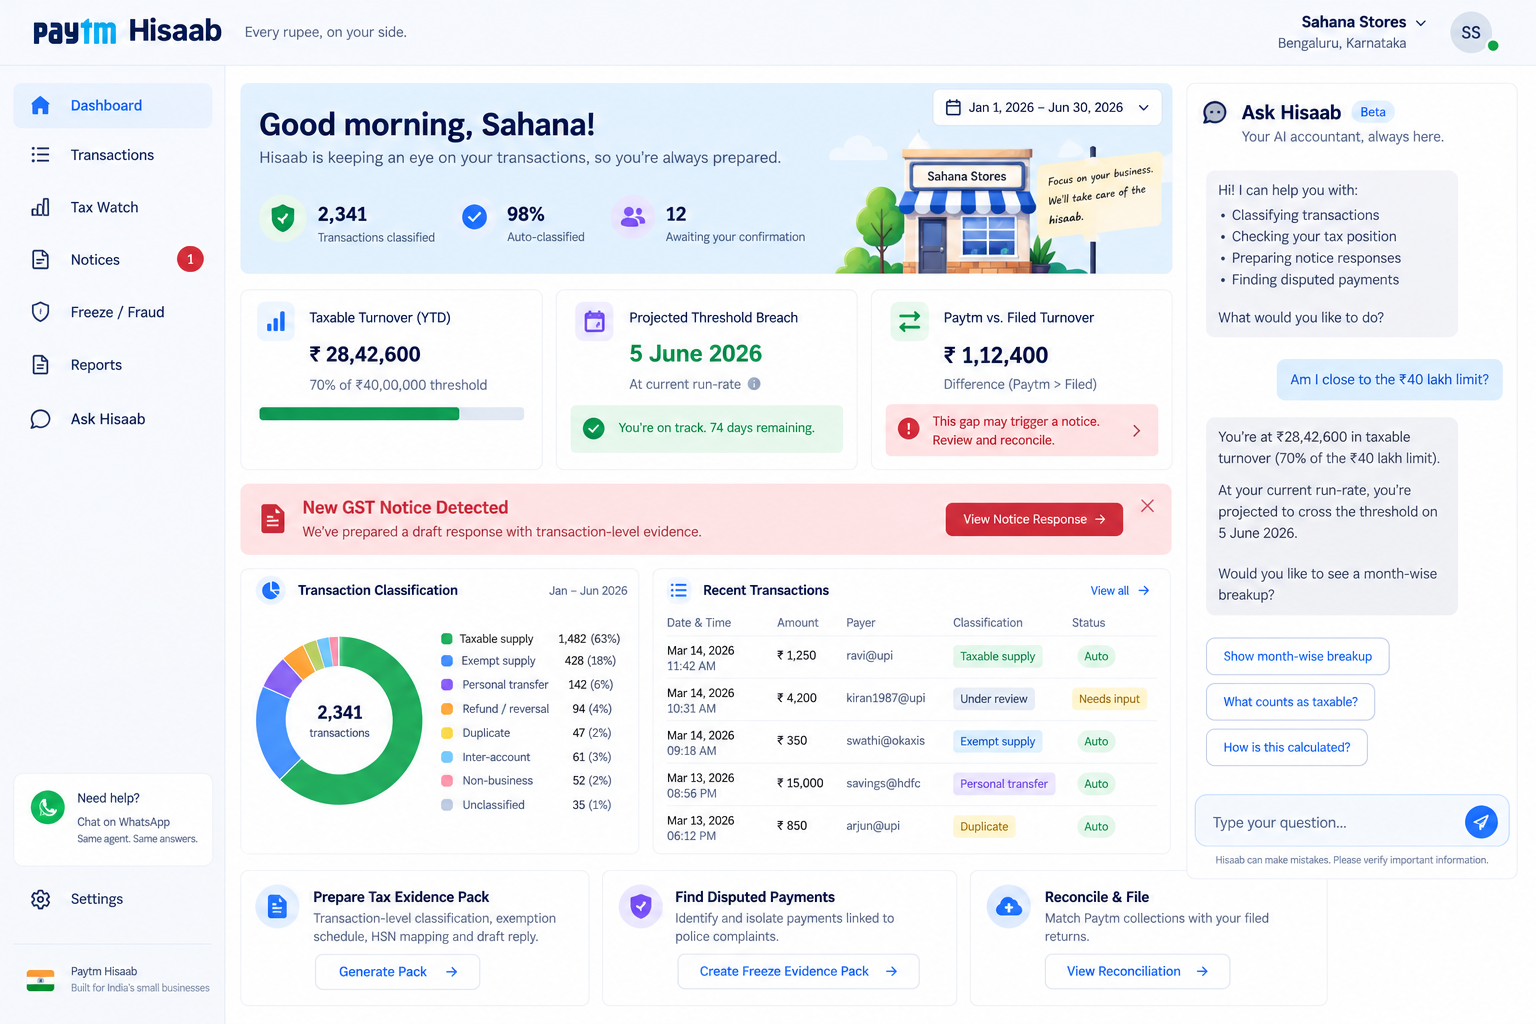
\includegraphics[width=\textwidth,height=0.70\textheight,keepaspectratio]{Paytm-Hisaab_website_look.png}
\end{center}
\vspace{0.1cm}
\hspace{0.05cm}{\scriptsize\color{muted}One surface: what every payment was classified as, how close she is to the threshold, and the packs. The same agent runs on WhatsApp, where she actually is.}
\note{{\color{navy}\bfseries\normalsize 8.~What the merchant sees}\par\vspace{0.55em}\textbf{0:20 --- a glance slide. Do not tour the UI.}
\\[0.4em]
One sentence: everything classified, how close she is to the threshold, and the
packs, on one surface.
\\[0.4em]
Then the WhatsApp point --- the same agent, where she actually is --- and advance.
\\[0.4em]
If someone asks whether this is built: the chat and the tools are live; this
screen is the product surface we are designing toward.}
\end{frame}

% ============================================================ 9. ARCHITECTURE
\begin{frame}{Built on Phinite}{Two agent graphs, four agents, ten deterministic skills}
\vspace{0.15cm}
\begin{columns}[T]
\begin{column}{0.53\textwidth}
{\scriptsize
\begin{tabular}{@{}L{1.75cm}L{4.7cm}@{}}
\multicolumn{2}{@{}l}{\color{navy}\bfseries\small hisaab-watch \;\scriptsize(autonomous: cron + API)}\\
\midrule
Provenance & proposes a tag and a reason for the hard credits \\
Evidence   & assembles packs: freeze evidence, then exemption schedules and HSN \\
\addlinespace[0.6em]
\multicolumn{2}{@{}l}{\color{navy}\bfseries\small hisaab-merchant \;\scriptsize(conversational: chat)}\\
\midrule
Merchant   & the conversation: attestation, alerts, Kannada \\
Escalation & decides when to stop and route to a human CA \\
\bottomrule
\end{tabular}}
\\[0.75em]
{\scriptsize\color{muted}The nightly pass writes its queue to the ledger; the chat reads it when she opens it. Deliberately \emph{not} a graph-to-graph call: a queue that outlives either run is what makes the handoff robust.}
\end{column}
\begin{column}{0.44\textwidth}
\card{5.7cm}{{\bfseries\color{navy}Permissions are the product}\\[0.4em]
\scriptsize Provenance proposes, \red{never commits}.\\[0.25em]
\scriptsize Merchant is the \emph{only} agent that can commit a tag.\\[0.25em]
\scriptsize Evidence is \red{read-only}. It cannot edit a classification to make a pack look better.\\[0.25em]
\scriptsize Escalation can \red{halt} any pack; a human approves.}
\\[0.5em]
\hspace{0.1cm}\begin{minipage}{5.7cm}{\scriptsize\color{muted}Ten tools run live against a hosted service. Every number in a pack traces back, in the trace, to the credit and the attestation behind it.}\end{minipage}
\end{column}
\end{columns}
\note{{\color{navy}\bfseries\normalsize 9.~Built on Phinite}\par\vspace{0.55em}\textbf{0:40 --- for the technical judges.}
\\[0.4em]
Two agent graphs, not four loose agents: \texttt{hisaab-watch} runs autonomously on
cron, \texttt{hisaab-merchant} is the conversation. The nightly pass writes a queue;
the chat reads it when she opens it --- deliberately not a graph-to-graph call,
because a queue that outlives either run is what makes the handoff robust.
\\[0.4em]
\textbf{Spend your time on the right-hand card.} The strongest line in it:
the Evidence agent is read-only --- \emph{the agent that builds the defence cannot
edit the evidence.} And only the Merchant agent can commit an attested tag.
\\[0.4em]
Those are enforced as Phinite tool policies, not conventions, and a denied call
shows up in the trace.}
\end{frame}

% ============================================================ 10. DESIGN DECISIONS
\begin{frame}{Four decisions that make it defensible}
\vspace{0.3cm}
\begin{columns}[T]
\begin{column}{0.48\textwidth}
\card{6.0cm}{{\bfseries\color{navy}1. Arithmetic lives in skills, not the model}\\[0.35em]
\scriptsize Turnover, projections and apportionment are deterministic Python: versioned, testable, traceable. Wrapping arithmetic in an LLM is the standard tell, and the trace would show it.}
\\[0.35em]
\card{6.0cm}{{\bfseries\color{navy}3. Refusing to guess is a feature}\\[0.35em]
\scriptsize An \texttt{unclassified} credit routed to the merchant costs one tap. A confident wrong tag inside an evidence pack is a catastrophe. We report the refusal rate honestly.}
\end{column}
\begin{column}{0.48\textwidth}
\card{6.0cm}{{\bfseries\color{navy}2. Attestation is the promotion boundary}\\[0.35em]
\scriptsize Nothing enters a production pack that the merchant has not confirmed. Sandbox to UAT to prod, with her tap as the gate.}
\\[0.35em]
\card{6.0cm}{{\bfseries\color{navy}4. Ground truth, so accuracy is a number}\\[0.35em]
\scriptsize We simulated a year of a shop's life from a known process, split into what Paytm can see and what really happened. Agents read only the visible half, which is why we quote error bars instead of vibes.}
\end{column}
\end{columns}
\note{{\color{navy}\bfseries\normalsize 10.~Four decisions}\par\vspace{0.55em}\textbf{0:35 --- the slide that separates you from a demo.}
\\[0.4em]
Lead with \#1: all arithmetic is deterministic Python, not model output. Wrapping
arithmetic in an LLM is the standard tell, and the trace would show it.
\\[0.4em]
Then \#3: refusing to guess is a feature. An \texttt{unclassified} credit costs one
tap; a confident wrong tag inside an evidence pack is a catastrophe.
\\[0.4em]
Skim \#2 and \#4 --- one clause each. \#4 is worth a beat if the room is technical:
we generated ground truth, so accuracy is a number instead of a claim.}
\end{frame}

% ============================================================ 11. DEMO / ATTESTATION
\begin{frame}{Demo $\cdot$ Sahana Stores, Jayanagar}{An ordinary Tuesday, before anything goes wrong}
\vspace{0.1cm}
\begin{columns}[T]
\begin{column}{0.48\textwidth}
{\scriptsize\color{muted}Tuesday 10 March. Thirty-nine credits came in over the weekend. The agent asks about \hi{three}.}
\\[0.4em]
\card{5.9cm}{{\kn\scriptsize ಭಾನುವಾರ ರಾತ್ರಿ ₹15,000. ನಿಮ್ಮ ಸ್ವಂತ ಹಣವೇ?}\\[0.25em]
{\color{muted}\scriptsize \qm{₹15,000 at 11:04pm Sunday, from your savings account. Your own money?}}\\[0.35em]
{\scriptsize\color{navy}\fbox{\kn ಹೌದು}\;\fbox{\kn ಇಲ್ಲ}}}
\\[0.4em]
{\scriptsize $\cdot$\; ₹7,500 from her husband, scanned at the shop QR\\[0.25em]
$\cdot$\; ₹4,850 from Raghu Shetty, who has bought twice before. A real sale, and the agent \emph{asks} rather than assumes.}
\\[0.4em]
{\scriptsize\color{muted}The other thirty-six settle silently, and a ₹23 payment nobody can place is left alone.}
\end{column}
\begin{column}{0.48\textwidth}
\ocard{amber}{6.1cm}{{\bfseries\color{amber}And yes, two of those three should not be there}\\[0.35em]
\scriptsize A business QR is not for personal money, and the terms say so. It arrives anyway: family, own top-ups, a chit payout. The rule does not prevent it. It only means \emph{nobody keeps a record of it.}}
\\[0.45em]
{\scriptsize Paytm already reads the signals: channel, linked VPAs, payer history. What no system has is the \hi{merchant's own answer}, given at the time, in her language, and kept.}
\\[0.45em]
{\scriptsize That record is what the next two slides are built from: first for the police, then for the department.}
\end{column}
\end{columns}
\note{{\color{navy}\bfseries\normalsize 11.~Demo --- an ordinary Tuesday (beat 1)}\par\vspace{0.55em}\textbf{0:45 --- or hand over to the live demo here.}
\\[0.4em]
Thirty-nine credits came in over the weekend, the agent asks about \textbf{three}.
Read the Kannada line if you can; otherwise read the gloss under it.
\\[0.4em]
\textbf{Do not hide from the right-hand card --- lead with it.} The mid-review
point was that personal money is not allowed on a business QR. Correct, and we say
so on the slide. The argument is that the rule does not stop it, it only means no
one records it, and an unrecorded credit is what an authority later reads as income.
\\[0.4em]
\textbf{Second half of that card matters just as much.} We are not claiming Paytm
does nothing. It already reads channel, linked VPAs and payer history. What no
system has is her own answer, captured while it is still knowable. That is the
product, and it is a smaller, truer claim than the one we started with.
\\[0.4em]
\textbf{Before going on stage:} confirm the attestation queue is whole ---
\texttt{pending\_total} must be 3. A rehearsal that taps through this beat spends the
queue, and Render needs a clear-cache redeploy to restore it.}
\end{frame}

% ============================================================ 12. DEMO / THE FREEZE
\begin{frame}{Demo $\cdot$ The emergency}{The account is frozen at 09:30 and the supplier payment is due}
\vspace{0.2cm}
\begin{columns}[T]
\begin{column}{0.46\textwidth}
{\scriptsize She sold someone 12kg of onions. That customer was three layers downstream of a fraud victim. She is not named in the FIR, which was filed in another state, and \hi{339 payments} came in that week.}
\\[0.5em]
\card{5.8cm}{{\bfseries\color{navy}The agent isolates it}\\[0.35em]
\scriptsize ₹4,200 on 21 March at 19:47, till POS01. Matched by UTR \emph{and independently} by amount and date.\\[0.3em]
\scriptsize The sale record comes with it: the POS bill, the items, the till and the minute.}
\end{column}
\begin{column}{0.49\textwidth}
\ocard{amber}{6.1cm}{{\bfseries\color{amber}And the decoy it did not choose}\\[0.35em]
\scriptsize A \emph{second} ₹4,200 that same week, from a regular customer. Listed in the pack, and explicitly \emph{not} named as the disputed one. Only the date separates them.}
\\[0.5em]
{\scriptsize Then it drafts the NCRP-CFCFRMS grievance, citing the judgments that only the \emph{disputed amount} should be lien-marked, not the whole account.}
\\[0.5em]
{\scriptsize\color{bad}\bfseries It never asserts that she is innocent.}\\[0.1em]
{\scriptsize\color{muted}Some frozen accounts genuinely are mule accounts. The agent assembles evidence; a human decides. Escalation holds the pack for approval.}
\end{column}
\end{columns}
\note{{\color{navy}\bfseries\normalsize 12.~Demo --- the emergency (beat 4)}\par\vspace{0.55em}\textbf{0:50 --- this is now the lead case. Give it the most time of the three.}
\\[0.4em]
Set the stakes in one sentence: account frozen at half nine, supplier payment due,
339 payments came in that week, and she is not named in the FIR.
\\[0.4em]
\textbf{Why this one leads.} She did nothing wrong and there is no rule she broke.
She sold onions to a customer who turned out to be laundering. Every objection
available against the tax case --- she should not have taken personal money on that
QR, she should have registered --- has no purchase here at all.
\\[0.4em]
The agent isolates ₹4,200 by UTR \emph{and independently} by amount and date, and
brings the POS bill with it --- the items, till POS01, 19:47.
\\[0.4em]
\textbf{The decoy is the point.} A second ₹4,200 that same week from a regular
customer, listed in the pack and explicitly not chosen. Anyone can match an amount;
the pack shows its work.
\\[0.4em]
Finish on the red line: it never asserts she is innocent. Some frozen accounts
genuinely are mule accounts. We assemble evidence; a human decides, and Escalation
holds the pack for approval.}
\end{frame}

% ============================================================ 13. DEMO / TAX
\begin{frame}{Demo $\cdot$ The warning, and the notice}{The same ledger, read for the other authority}
\vspace{0.15cm}
\begin{columns}[T]
\begin{column}{0.38\textwidth}
{\scriptsize\color{muted}Replayed as of 31 January:}
\\[0.35em]
\ocard{good}{4.8cm}{{\bfseries\color{ink}\scriptsize\qm{At your current rate you cross ₹40 lakh around {\color{bad}14 March}. You will need to register.}}\\[0.35em]
{\scriptsize\color{muted}\grn{43 days of warning}, and the date is computed, not typed.}}
\\[0.45em]
{\scriptsize\color{bad}\bfseries This beat is what makes the pitch safe.}\\[0.1em]
{\scriptsize\color{muted}Its first act on the tax side is telling her to register.}
\end{column}
\begin{column}{0.58\textwidth}
{\scriptsize\color{muted}Then the notice arrives, claiming {\color{bad}\bfseries ₹60.98L} of turnover:}
\\[0.3em]
{\scriptsize
\begin{tabular}{@{}lr@{\hskip 1.2em}l@{}}
\multicolumn{2}{@{}l}{\color{navy}\bfseries Aggregate turnover \quad ₹42.2L} & \sub{within \grn{1.6\%} of truth} \\
\midrule
Exempt supplies      & ₹31.3L & \sub{vegetables, loose rice} \\
Taxable supplies     & ₹10.9L & \sub{branded goods, oil, soap} \\
\addlinespace[0.45em]
\multicolumn{2}{@{}l}{\color{navy}\bfseries Not turnover at all \quad ₹18.8L} & \sub{every line traced} \\
\midrule
Her own accounts     & ₹7.4L & \sub{top-ups before supplier runs} \\
Family               & ₹6.1L & \sub{spouse, parent, in-law} \\
Loans, chit, gifts   & ₹4.3L & \sub{chit payout, festival gifts} \\
Refunds, duplicates  & ₹1.0L & \sub{crate returns, double-taps} \\
\bottomrule
\end{tabular}}
\\[0.45em]
{\scriptsize And it says plainly: \hi{the claim is wrong, and you \emph{did} cross ₹40 lakh on 14 March. You must register.}}
\end{column}
\end{columns}
\note{{\color{navy}\bfseries\normalsize 13.~Demo --- the warning and the notice (beats 2 and 3)}\par\vspace{0.55em}\textbf{0:50 --- two tax beats on one slide, deliberately compressed.}
\\[0.4em]
Left: replayed as of 31 January, the agent says she crosses ₹40 lakh around
14 March. \textbf{Say the red line out loud} --- its first act on the tax side is
telling her she owes a registration. That is what stops the room turning hostile.
\\[0.4em]
Right: the notice claims ₹60.98 lakh, and the pack answers it line by line, every
figure traceable to transaction IDs. Then the honest half:
\textbf{the claim is wrong, and she did cross ₹40 lakh, and she must register.}
\\[0.4em]
\textbf{If a judge diffs this against slide 5:} slide 5 shows seeded truth
(₹42.9L), this shows what our system computed (₹42.2L). The 1.6\% between them
\emph{is} the accuracy claim --- say that, do not hedge.
\\[0.4em]
\textbf{If pushed on the personal and own-account lines:} same answer as slide 11.
Those credits should not be on a business QR, they are there anyway, and the
alternative to classifying them is letting them be read as income.}
\end{frame}

% ============================================================ 14. NUMBERS
\begin{frame}{What we can actually prove}{One merchant, one year, 13,267 credits, scored against seeded truth}
\vspace{0.45cm}
\begin{columns}[T]
\begin{column}{0.33\textwidth}
\begin{center}\bignum{1.6\%}{error on aggregate turnover\\ (taxable share within 1\%)}\end{center}
\vspace{0.55cm}
\begin{center}\bignum{43 days}{of warning before the\\ threshold crossing}\end{center}
\end{column}
\begin{column}{0.33\textwidth}
\begin{center}\bignum{1.3 a day}{median questions asked.\\ 189 in a year, never over 3}\end{center}
\vspace{0.55cm}
\begin{center}\bignum{zero}{credits left untagged\\ across the whole year}\end{center}
\end{column}
\begin{column}{0.30\textwidth}
\card{3.8cm}{{\bfseries\color{navy}The honest baseline}\\[0.35em]
\scriptsize A 50-line rules-only classifier gets 99.3\% on sale vs not-a-sale, but catches only \red{77.8\%} of non-sale credits.\\[0.3em]
\scriptsize That residue alone puts two eval merchants on the \emph{wrong side} of ₹40L.\\[0.3em]
\scriptsize Closing it is what the agent plus one tap is for.}
\end{column}
\end{columns}
\vspace{0.45cm}
\hspace{0.1cm}{\scriptsize\color{muted}She corrected the agent 52 times that year. Those corrections are the ledger's strongest evidence, not its failures.}
\note{{\color{navy}\bfseries\normalsize 14.~What we can actually prove}\par\vspace{0.55em}\textbf{0:30 --- do not read all four. Pick two.}
\\[0.4em]
Lead with \textbf{1.6\%} error on turnover and \textbf{1.3 questions a day}. The
other two are there to be read, not narrated.
\\[0.4em]
\textbf{The credibility move is the box on the right} --- volunteer the weakness
before anyone finds it. A rules-only baseline gets 99.3\% on sale vs not-a-sale
but catches only 77.8\% of non-sale credits, and that residue alone puts two eval
merchants on the wrong side of ₹40 lakh. Closing it is what the agent plus one tap is for.
\\[0.4em]
Last line if you have the beat: she corrected the agent 52 times that year, and
those corrections are the ledger's strongest evidence, not its failures.}
\end{frame}

% ============================================================ 15. CLOSE
\begin{frame}{The line we do not cross}{Accuracy, not minimisation}
\vspace{0.3cm}
\begin{columns}[T]
\begin{column}{0.52\textwidth}
{\scriptsize
$\cdot$\; We \hi{never assert innocence} on a freeze. Some accounts really are mule accounts. We assemble evidence; a human decides.\\[0.5em]
$\cdot$\; We \hi{file nothing} with any authority. Artefacts only; the merchant or their CA files.\\[0.5em]
$\cdot$\; We compute what she \hi{genuinely owes} and say so plainly, including \qm{you crossed the threshold, you must register.}\\[0.5em]
$\cdot$\; We \hi{never assert a final liability}. We compute, show the workings, and route to a CA.\\[0.5em]
$\cdot$\; A business QR is \hi{not for personal money}. We do not excuse it. We record it, so it is not read as income.}
\end{column}
\begin{column}{0.44\textwidth}
\begin{tikzpicture}\node[rounded corners=4pt,fill=navy,text=white,inner sep=10pt,text width=5.7cm,align=left]{
{\bfseries Why this has to be Paytm}\\[0.45em]
\scriptsize The rail is the only place provenance is cheap. Everyone else arrives eighteen months late, when the answer is already unrecoverable.\\[0.45em]
\scriptsize A frozen merchant cannot transact at all: dead Soundbox and zero GMV the same morning, before it becomes the sign on the shutter, \emph{\qm{No UPI. Cash only.}}
};\end{tikzpicture}
\end{column}
\end{columns}
\vspace{0.4cm}
\begin{center}
{\large\color{navy}\bfseries Paytm Hisaab}\quad{\color{muted}every rupee, on your side.}
\end{center}
\note{{\color{navy}\bfseries\normalsize 15.~The line we do not cross}\par\vspace{0.55em}\textbf{0:30 --- the non-negotiables, fast, then land.}
\\[0.4em]
Run the five bullets at pace. The one to hit is the first: we never assert
innocence on a freeze. The last is the mid-review answer, on the slide on purpose.
\\[0.4em]
Then the navy box: provenance is cheap only on the rail, and a frozen merchant
stops transacting the same morning.
\\[0.4em]
Final line, unhurried: \emph{``Paytm Hisaab. Every rupee, on your side.''} Stop talking.
\\[0.5em]
{\scriptsize
{\color{navy}\bfseries --- Q\&A prep ---}
\\[0.3em]
\textbf{``Merchants may not take personal money on a business QR.''} Correct, and
slide 11 says so before you have to. It arrives anyway, and the alternative to
recording it is letting an authority read it as income. We are not defending the
behaviour --- we are refusing to let it become a liability.
\\[0.3em]
\textbf{``Paytm already tags transactions.''} It does, and we build on that rather
than around it: channel, linked VPAs and payer history feed the rules layer. What
no tag carries is her attestation --- the part an authority accepts, and the only
part she alone can give.
\\[0.3em]
\textbf{``No return mismatch?''} That check needs a \emph{registered} composition
dealer who filed a CMP-08 to disagree with. Ours is unregistered, which is why she
gets a notice at all; the eval split has one with four quarters seeded.
\\[0.3em]
\textbf{``Exempt vs taxable on a QR sale?''} Not per payment. We apportion by value
from that shop's own POS-billed ratio and label it an estimate. Labelling each sale
by its majority side understated taxable turnover threefold.
\\[0.3em]
\textbf{``Four LLM calls in a trenchcoat?''} Everything deterministic is a skill and
four agents is the ceiling. If twenty lines of Python replaces an agent, it should
have been a skill --- the trace shows which is which.
\\[0.3em]
\textbf{``No standing with the police.''} Agreed: Paytm supplies, the merchant
files. By design. Cash sales are real, out of scope, and on the slide.}}
\end{frame}

\end{document}
"
%                                                     -> speaker notes, one page per slide
%
% Speaker notes live in the \note{} after each frame, so they cannot drift
% out of sync with the slides. Build both with: ./build.sh
%
% Fonts: Segoe UI + Nirmala UI (both ship with Windows). On another OS the
% deck still builds -- it falls back to the default sans and drops the
% Kannada styling.
\documentclass[aspectratio=169,10pt]{beamer}

\usepackage{fontspec}
\usepackage{tikz}
\usepackage{booktabs}
\usepackage{array}
\newcolumntype{L}[1]{>{\raggedright\arraybackslash}p{#1}}
\usepackage{graphicx}
\usetikzlibrary{calc,positioning,arrows.meta}

\graphicspath{{./}{../}}

% ---------- fonts ----------
\IfFontExistsTF{Segoe UI}{\setsansfont{Segoe UI}}{}
\IfFontExistsTF{Nirmala UI}{%
  \newfontfamily\kn[Script=Kannada]{Nirmala UI}}{%
  \newcommand{\kn}{}}
\renewcommand{\familydefault}{\sfdefault}

% ragged, unhyphenated text inside the narrow cards
\hyphenpenalty=10000
\exhyphenpenalty=10000
\emergencystretch=3em
\hbadness=10000

% ---------- palette (taken from the product mock) ----------
\definecolor{navy}{HTML}{002970}
\definecolor{ptmcyan}{HTML}{00BAF2}
\definecolor{ink}{HTML}{0F172A}
\definecolor{muted}{HTML}{64748B}
\definecolor{good}{HTML}{15803D}
\definecolor{bad}{HTML}{DC2626}
\definecolor{amber}{HTML}{B45309}
\definecolor{tint}{HTML}{EAF4FD}
\definecolor{hairline}{HTML}{DBE7F3}

% ---------- theme ----------
\usetheme{default}
\usecolortheme{default}
\setbeamertemplate{navigation symbols}{}
\setbeamersize{text margin left=0.85cm,text margin right=0.85cm}
\setbeamercolor{normal text}{fg=ink,bg=white}
\setbeamercolor{frametitle}{fg=navy}
\setbeamercolor{structure}{fg=navy}
\setbeamerfont{frametitle}{size=\large,series=\bfseries}
\setbeamerfont{framesubtitle}{size=\scriptsize}
\setbeamercolor{framesubtitle}{fg=muted}
\setbeamertemplate{frametitle}{%
  \vspace{0.30cm}%
  \usebeamerfont{frametitle}\usebeamercolor[fg]{frametitle}\insertframetitle%
  \ifx\insertframesubtitle\empty\else{\\[-0.15em]\usebeamerfont{framesubtitle}\usebeamercolor[fg]{framesubtitle}\insertframesubtitle}\fi%
  \\[0.1em]{\color{ptmcyan}\rule{1.2cm}{2pt}}\par\vspace{-0.15em}%
}
\setbeamertemplate{footline}{%
  \hbox{\begin{beamercolorbox}[wd=\paperwidth,ht=1.9ex,dp=1.1ex,leftskip=0.85cm,rightskip=0.85cm]{}%
  {\scriptsize\color{muted}Paytm Hisaab\hfill\insertframenumber}%
  \end{beamercolorbox}}%
}
\setbeamerfont{itemize/enumerate body}{size=\normalsize}

% ---------- helpers ----------
\newcommand{\hi}[1]{{\color{navy}\bfseries #1}}
\newcommand{\red}[1]{{\color{bad}\bfseries #1}}
\newcommand{\grn}[1]{{\color{good}\bfseries #1}}
\newcommand{\sub}[1]{{\color{muted}#1}}
\newcommand{\qm}[1]{``#1''}
\newcommand{\bignum}[2]{{\color{navy}\fontsize{22}{24}\selectfont\bfseries #1}\\[0.1em]{\scriptsize\color{muted}#2}}
% a soft rounded card:  \card{width}{body}
\newcommand{\card}[2]{\begin{tikzpicture}%
  \node[rounded corners=4pt,fill=tint,inner sep=8pt,text width=#1,align=left]{#2};%
  \end{tikzpicture}}
% an outlined card:  \ocard{colour}{width}{body}
\newcommand{\ocard}[3]{\begin{tikzpicture}%
  \node[rounded corners=4pt,fill=white,draw=#1,line width=0.9pt,inner sep=8pt,text width=#2,align=left]{#3};%
  \end{tikzpicture}}

% ---------- presenter build ----------
% Set after every colour and template above, so the composed notes page keeps
% the deck's own colours:
%   xelatex -jobname=hisaab-pitch-notes "\def\shownotes{1}% Paytm Hisaab -- buildathon pitch deck
%
% Compile with XeLaTeX (needed for the rupee sign and the Kannada line):
%
%   cd pitch
%   xelatex hisaab-pitch.tex                          -> hisaab-pitch.pdf  (slides)
%   xelatex -jobname=hisaab-pitch-notes "\def\shownotes{1}\input{hisaab-pitch.tex}"
%                                                     -> speaker notes, one page per slide
%
% Speaker notes live in the \note{} after each frame, so they cannot drift
% out of sync with the slides. Build both with: ./build.sh
%
% Fonts: Segoe UI + Nirmala UI (both ship with Windows). On another OS the
% deck still builds -- it falls back to the default sans and drops the
% Kannada styling.
\documentclass[aspectratio=169,10pt]{beamer}

\usepackage{fontspec}
\usepackage{tikz}
\usepackage{booktabs}
\usepackage{array}
\newcolumntype{L}[1]{>{\raggedright\arraybackslash}p{#1}}
\usepackage{graphicx}
\usetikzlibrary{calc,positioning,arrows.meta}

\graphicspath{{./}{../}}

% ---------- fonts ----------
\IfFontExistsTF{Segoe UI}{\setsansfont{Segoe UI}}{}
\IfFontExistsTF{Nirmala UI}{%
  \newfontfamily\kn[Script=Kannada]{Nirmala UI}}{%
  \newcommand{\kn}{}}
\renewcommand{\familydefault}{\sfdefault}

% ragged, unhyphenated text inside the narrow cards
\hyphenpenalty=10000
\exhyphenpenalty=10000
\emergencystretch=3em
\hbadness=10000

% ---------- palette (taken from the product mock) ----------
\definecolor{navy}{HTML}{002970}
\definecolor{ptmcyan}{HTML}{00BAF2}
\definecolor{ink}{HTML}{0F172A}
\definecolor{muted}{HTML}{64748B}
\definecolor{good}{HTML}{15803D}
\definecolor{bad}{HTML}{DC2626}
\definecolor{amber}{HTML}{B45309}
\definecolor{tint}{HTML}{EAF4FD}
\definecolor{hairline}{HTML}{DBE7F3}

% ---------- theme ----------
\usetheme{default}
\usecolortheme{default}
\setbeamertemplate{navigation symbols}{}
\setbeamersize{text margin left=0.85cm,text margin right=0.85cm}
\setbeamercolor{normal text}{fg=ink,bg=white}
\setbeamercolor{frametitle}{fg=navy}
\setbeamercolor{structure}{fg=navy}
\setbeamerfont{frametitle}{size=\large,series=\bfseries}
\setbeamerfont{framesubtitle}{size=\scriptsize}
\setbeamercolor{framesubtitle}{fg=muted}
\setbeamertemplate{frametitle}{%
  \vspace{0.30cm}%
  \usebeamerfont{frametitle}\usebeamercolor[fg]{frametitle}\insertframetitle%
  \ifx\insertframesubtitle\empty\else{\\[-0.15em]\usebeamerfont{framesubtitle}\usebeamercolor[fg]{framesubtitle}\insertframesubtitle}\fi%
  \\[0.1em]{\color{ptmcyan}\rule{1.2cm}{2pt}}\par\vspace{-0.15em}%
}
\setbeamertemplate{footline}{%
  \hbox{\begin{beamercolorbox}[wd=\paperwidth,ht=1.9ex,dp=1.1ex,leftskip=0.85cm,rightskip=0.85cm]{}%
  {\scriptsize\color{muted}Paytm Hisaab\hfill\insertframenumber}%
  \end{beamercolorbox}}%
}
\setbeamerfont{itemize/enumerate body}{size=\normalsize}

% ---------- helpers ----------
\newcommand{\hi}[1]{{\color{navy}\bfseries #1}}
\newcommand{\red}[1]{{\color{bad}\bfseries #1}}
\newcommand{\grn}[1]{{\color{good}\bfseries #1}}
\newcommand{\sub}[1]{{\color{muted}#1}}
\newcommand{\qm}[1]{``#1''}
\newcommand{\bignum}[2]{{\color{navy}\fontsize{22}{24}\selectfont\bfseries #1}\\[0.1em]{\scriptsize\color{muted}#2}}
% a soft rounded card:  \card{width}{body}
\newcommand{\card}[2]{\begin{tikzpicture}%
  \node[rounded corners=4pt,fill=tint,inner sep=8pt,text width=#1,align=left]{#2};%
  \end{tikzpicture}}
% an outlined card:  \ocard{colour}{width}{body}
\newcommand{\ocard}[3]{\begin{tikzpicture}%
  \node[rounded corners=4pt,fill=white,draw=#1,line width=0.9pt,inner sep=8pt,text width=#2,align=left]{#3};%
  \end{tikzpicture}}

% ---------- presenter build ----------
% Set after every colour and template above, so the composed notes page keeps
% the deck's own colours:
%   xelatex -jobname=hisaab-pitch-notes "\def\shownotes{1}\input{hisaab-pitch.tex}"
\ifdefined\shownotes
  \setbeamertemplate{note page}{%
    \usebeamercolor[fg]{normal text}%
    \vspace{0.2em}%
    {\scriptsize\color{muted}Paytm Hisaab \;$\cdot$\; speaker notes}\hfill
    {\scriptsize\color{muted}slide \insertframenumber\ of 15}\par
    \vspace{0.25em}{\color{ptmcyan}\rule{\textwidth}{1.5pt}}\par
    \vspace{0.55em}\footnotesize\raggedright\insertnote\par}
  \setbeameroption{show only notes}
\fi

\begin{document}

% ============================================================ 1. TITLE
{\setbeamertemplate{footline}{}
\begin{frame}[plain]
\vspace{0.9cm}
\begin{center}
{\fontsize{38}{42}\selectfont\bfseries\color{navy}Paytm\;\color{ink}Hisaab}\\[0.45em]
{\Large\color{muted}Every rupee, on your side.}\\[0.9em]
{\color{ptmcyan}\rule{2.8cm}{2.5pt}}\\[0.9em]
{\large\color{ink}The agent that lets a merchant account for their own money}\\[0.15em]
{\large\color{ink}when someone in authority demands an explanation.}\\[1.3em]
{\small\color{muted}Agent Labs Buildathon \;$\cdot$\; Phinite $\times$ Paytm \;$\cdot$\; Track 2: AI for Small Businesses}
\end{center}
\note{{\color{navy}\bfseries\normalsize 1.~Title}\par\vspace{0.55em}\textbf{0:10 --- open cold.} Do not read the title or the tagline off the slide.
\\[0.4em]
Say: \emph{``I want to tell you about a man in Haveri who opened an envelope.''} Then advance.
\\[0.4em]
Nothing on this slide needs explaining. The tagline lands at the end, not here.}
\end{frame}}

% ============================================================ 2. STORY
\begin{frame}{Haveri, 2025}{A vegetable vendor opens an envelope}
\vspace{0.05cm}
\begin{columns}[T]
\begin{column}{0.52\textwidth}
\vspace{0.15cm}
He sells vegetables. Vegetables are \hi{exempt} from GST.\\[0.6em]
He also took UPI, because Paytm asked him to.\\[0.6em]
Four years of credits into his account, added up and billed as income:
\begin{center}\vspace{0.1em}{\fontsize{30}{32}\selectfont\bfseries\color{bad}₹29 lakh}\end{center}
\end{column}
\begin{column}{0.44\textwidth}
\ocard{hairline}{5.4cm}{\centering
  {\color{muted}\scriptsize Within weeks, on shutters across Karnataka:}\\[0.6em]
  {\fontsize{20}{23}\selectfont\bfseries\color{ink}\qm{No UPI.\\ Cash only.}}\\[0.6em]
  {\color{muted}\scriptsize A statewide boycott, by the merchants who had just adopted it.}}
\end{column}
\end{columns}
\vspace{0.25cm}
\hspace{0.1cm}{\small\sub{Withdrawn for the traders who could \emph{show} what they sold. Most could not. And tax is no longer the only authority asking.}}
\note{{\color{navy}\bfseries\normalsize 2.~Haveri, 2025}\par\vspace{0.55em}\textbf{0:45 --- the hook. Tell it, do not summarise it.}
\\[0.4em]
Four beats, in this order: he sells vegetables; vegetables are exempt from GST;
he took UPI because \emph{we} asked him to; the department added up four years of
credits and sent him a bill for \textbf{₹29 lakh}.
\\[0.4em]
\textbf{Pause on the number.} Then the card: within weeks, shutters across Karnataka
read ``No UPI, cash only.'' Merchants we had just onboarded, boycotting the rail.
\\[0.4em]
Close on the bottom line --- the notices were withdrawn for traders who could
\emph{show} what they sold. Most could not. That verb is the whole product.
\\[0.4em]
\textbf{Then the bridge:} \emph{``and tax is no longer the only authority asking.''}
That sentence is doing the repositioning --- Haveri is not a tax story here, it is
the moment taking digital money became a liability. The sharper version of it is
two slides away.
\\[0.4em]
\textbf{Do not say this is happening right now.} It is 2025. The next slide is
what makes it current, and a judge who knows the episode will respect the distinction.}
\end{frame}

% ============================================================ 3. STILL HAPPENING
\begin{frame}{And this is not a 2025 story}{CAclubindia, last updated 02 September 2026: ten days ago}
\vspace{0.1cm}
\begin{center}

\includegraphics[width=12.4cm]{gst-notices-2026.png}
\end{center}
\vspace{0.35cm}
\card{13.1cm}{\scriptsize\qm{During August 2026, the GST Department issued a significant number of notices covering different financial years and involving a wide range of issues\ldots\ They covered matters such as ITC mismatches, ineligible credit, \hi{differences in turnover}, wrong GST classification or rate, \hi{exemption claims}, Reverse Charge Mechanism\ldots}}
\vspace{0.3cm}

\hspace{0.1cm}{\small Those two categories are the whole content of an evidence pack. And this is the \emph{slower} of the two authorities. The other one freezes the account first.}
\note{{\color{navy}\bfseries\normalsize 3.~And this is not a 2025 story}\par\vspace{0.55em}\textbf{0:25 --- fast. This slide exists to kill one objection.}
\\[0.4em]
Say: \emph{``That was last year. This was published ten days ago.''}
\\[0.4em]
Do not read the quote. Point at the two bolded phrases only ---
\textbf{differences in turnover} and \textbf{exemption claims} --- and say those
two categories are the entire content of what we build.
\\[0.4em]
\textbf{Land on the last line and move.} It is the handoff into the police
slide: this is the slower authority. The other one freezes first and asks
afterwards. Do not linger here --- tax is no longer the headline.}
\end{frame}

% ============================================================ 4. THE TRAP
\begin{frame}{Every rupee a merchant receives is now evidence}{Today it is only ever used against them}
\vspace{0.05cm}
\begin{columns}[T]
\begin{column}{0.47\textwidth}
\ocard{bad}{6.0cm}{{\bfseries\color{bad}The cyber-crime police}\\[0.35em]
\scriptsize Fraud money layers through accounts within minutes. The shop at the end of the chain, the one that sold someone a watermelon, is frozen. It did nothing wrong, is not named in the FIR, and finds out when a payment declines.}
\end{column}
\begin{column}{0.47\textwidth}
\card{6.1cm}{{\bfseries\color{navy}The tax department}\\[0.35em]
\scriptsize Compares UPI collections against filed returns and bills the difference. Registered traders too, with QR, wallet, card and cash deposits all in scope.}
\end{column}
\end{columns}
\vspace{0.4cm}
\begin{center}
{\large Both demand the same artefact: \hi{what was each rupee, actually?}}\\[0.3em]
{\small\color{muted}Paytm already sees more of this than anyone. What is missing is the \emph{merchant's own answer}, captured when it is still knowable.}
\end{center}
\vspace{0.15cm}
{\color{hairline}\hrule height 1pt}
\vspace{0.35em}
\hspace{0.05cm}{\scriptsize\bfseries\color{bad}What it costs Paytm:}~{\scriptsize a frozen merchant stops transacting that morning. A frightened one takes the QR down for good. Dead Soundbox, zero GMV, no lending origination.}
\note{{\color{navy}\bfseries\normalsize 4.~Every rupee is now evidence}\par\vspace{0.55em}\textbf{0:40 --- two authorities, one unanswerable question.}
\\[0.4em]
\textbf{Left card first and give it the time.} Fraud money layers within minutes,
and the shop at the end of the chain, \emph{the one that sold someone a watermelon},
gets frozen. It did nothing wrong, it is not named in the FIR, and it finds out
when a payment declines. Use the watermelon.
\\[0.4em]
Right card briskly: the department reconciles collections against filed returns
and bills the difference. One sentence, then move.
\\[0.4em]
Then the pivot: both demand the same artefact --- what was each rupee, actually.
\\[0.4em]
\textbf{Say the grey line as written.} We do \emph{not} claim Paytm does nothing
with this data --- it tags plenty. The gap is the merchant's own answer, captured
when it is still knowable. Claiming otherwise in this room gets corrected.
\\[0.4em]
\textbf{Slow down for the red line.} This is the business case, not a footnote:
a frozen merchant stops transacting that morning, a frightened one takes the QR
down for good. Dead Soundbox, zero GMV, no lending origination.}
\end{frame}

% ============================================================ 5. THE BAR
\begin{frame}{Gross credits are not turnover}{One shop, one year, ₹60.98 lakh of credits}
\vspace{0.1cm}
\begin{center}
\begin{tikzpicture}[x=1cm,y=1cm]
% --- what the notice counts
\node[anchor=west,font=\scriptsize\bfseries,text=bad] at (-0.05,1.80) {WHAT THE NOTICE COUNTS AS TURNOVER};
\fill[bad!85,rounded corners=2pt] (0,1.06) rectangle (11.4,1.60);
\node[font=\small\bfseries,text=white] at (5.7,1.33) {₹60.98 lakh};

% --- what actually happened   (1 lakh = 0.18696 cm, so the bars are the same length)
\node[anchor=west,font=\scriptsize\bfseries,text=navy] at (-0.05,0.66) {WHAT ACTUALLY HAPPENED};
\fill[good!80,rounded corners=2pt]  (0,-0.08)     rectangle (6.001,0.46);
\fill[good!45]                      (6.001,-0.08) rectangle (8.002,0.46);
\fill[ptmcyan!70]                   (8.002,-0.08) rectangle (9.385,0.46);
\fill[navy!55]                      (9.385,-0.08) rectangle (10.451,0.46);
\fill[amber!70]                     (10.451,-0.08)rectangle (11.255,0.46);
\fill[muted!60,rounded corners=2pt] (11.255,-0.08)rectangle (11.4,0.46);

% brackets
\draw[navy,line width=0.8pt] (0,-0.22) -- (0,-0.36) -- (8.002,-0.36) -- (8.002,-0.22);
\node[anchor=north,font=\scriptsize,text=navy,align=center] at (4.0,-0.38)
  {\bfseries ₹42.9L aggregate turnover\quad{\color{muted}\scriptsize exempt ₹32.1L + taxable ₹10.7L}};
\draw[bad,line width=0.8pt] (8.002,-0.22) -- (8.002,-0.36) -- (11.4,-0.36) -- (11.4,-0.22);
\node[anchor=north,font=\scriptsize,text=bad,align=center] at (9.7,-0.38)
  {\bfseries ₹18.1L that is not turnover at all};

% legend
\node[font=\scriptsize,text=ink] at (5.7,-1.02) {%
\textcolor{good!80}{$\blacksquare$}~Exempt sales \quad
\textcolor{good!45}{$\blacksquare$}~Taxable sales \quad
\textcolor{ptmcyan!70}{$\blacksquare$}~Her own accounts ₹7.4L};
\node[font=\scriptsize,text=ink] at (5.7,-1.40) {%
\textcolor{navy!55}{$\blacksquare$}~Family ₹5.7L \quad
\textcolor{amber!70}{$\blacksquare$}~Loans, chit, gifts ₹4.3L \quad
\textcolor{muted!60}{$\blacksquare$}~Refunds \& duplicates ₹0.7L};
\end{tikzpicture}
\end{center}
\vspace{0.15cm}
\hspace{0.1cm}{\small\sub{Personal money does not belong on a business QR. It arrives anyway, reads as turnover, and hides the one credit the police will ask about.}}
\note{{\color{navy}\bfseries\normalsize 5.~Gross credits are not turnover}\par\vspace{0.55em}\textbf{0:45 --- the hinge of the pitch. Let the picture work.}
\\[0.4em]
Say: \emph{``One shop, one year, ₹60.98 lakh of credits. The red bar is what the
notice counts as turnover --- all of it.''}
\\[0.4em]
Then the bottom bar. \textbf{Stop talking for two seconds} and let them read it.
\\[0.4em]
₹42.9L really is turnover, and we say so. ₹18.1L is not: her savings account, her
husband, a chit payout, a double-tap on the Soundbox.
\\[0.4em]
\textbf{Get in front of the obvious objection.} Personal money is not supposed to
touch a business QR. Say so first, then say it arrives anyway --- that is an
observation about merchants, not a loophole we are selling. The rule does not stop
it; it only means no one is keeping a record of it.
\\[0.4em]
\textbf{And close on the second use.} This volume is also why she cannot find the
one credit the police care about. Same bar, same problem, and the freeze slide
pays it off.
\\[0.4em]
If challenged on the numbers: seeded ground truth from our generator, not an
estimate. Accuracy against it is slide 14.}
\end{frame}

% ============================================================ 6. INSIGHT
\begin{frame}{The insight}{Most teams would build the tax tool \emph{or} the fraud tool. They are the same engine.}
\vspace{0.15cm}
\begin{center}
\begin{tikzpicture}[font=\scriptsize]
\node[rounded corners=4pt,fill=navy,text=white,inner sep=7pt,align=center,text width=3.5cm]
  (eng) {\bfseries\small Provenance Ledger\\[0.15em] a merchant-attested label on every incoming credit};
\node[rounded corners=4pt,fill=tint,draw=bad,inner sep=6pt,align=center,text width=4.0cm]
  (tax) at ($(eng.east)+(3.7,0.78)$) {\bfseries The disputed rupee\\ freeze pack, NCRP grievance};
\node[rounded corners=4pt,fill=tint,draw=hairline,inner sep=6pt,align=center,text width=4.0cm]
  (fra) at ($(eng.east)+(3.7,-0.78)$) {\bfseries Defensible turnover\\ threshold watch, notice pack};
\draw[-{Stealth[length=2.5mm]},ptmcyan,line width=1.3pt] (eng.east) -- ++(0.5,0) |- (tax.west);
\draw[-{Stealth[length=2.5mm]},ptmcyan,line width=1.3pt] (eng.east) -- ++(0.5,0) |- (fra.west);
\node[anchor=east,text width=2.9cm,align=right,text=muted] at ($(eng.west)+(-0.35,0)$)
  {Both are downstream \emph{reads} of one ledger. Two output formats, not two products.};
\end{tikzpicture}
\end{center}
\vspace{0.1cm}
\begin{center}
\begin{tikzpicture}\node[rounded corners=4pt,fill=tint,inner sep=8pt,text width=11.2cm,align=center]{
{\bfseries\color{navy}The wedge nobody else has.}\\[0.25em]
\small Khatabook and Vyapar keep books after the fact. ClearTax files after the fact.\\
Neither sits on the rail \emph{at the moment money moves}. Paytm does.\\[0.25em]
\small Classification is cheap at the instant of the transaction,\\ and unrecoverable eighteen months later.
};\end{tikzpicture}
\end{center}
\note{{\color{navy}\bfseries\normalsize 6.~The insight}\par\vspace{0.55em}\textbf{0:40 --- why this is one product, not two.}
\\[0.4em]
Say: \emph{``Most teams would build the fraud tool or the tax tool. They are the
same engine.''} Both are downstream reads of one ledger --- two output formats,
and the freeze pack is the one we lead with.
\\[0.4em]
Then the wedge, and say it slowly because it is the defensible-moat answer:
Khatabook and Vyapar keep books after the fact, ClearTax files after the fact.
Neither sits on the rail at the moment money moves. \textbf{Paytm does.}
\\[0.4em]
Landing line: classification is cheap and accurate at the instant of the
transaction, and unrecoverable eighteen months later when the notice arrives.}
\end{frame}

% ============================================================ 7. THE ENGINE
\begin{frame}{The engine}{Eight tags, one tap}
\vspace{0.15cm}
\begin{columns}[T]
\begin{column}{0.45\textwidth}
{\color{navy}\bfseries\small Every incoming credit gets one tag}\\[0.4em]
{\scriptsize
\begin{tabular}{@{}ll@{}}
\texttt{taxable\_supply}    & ordinary sale \\
\texttt{exempt\_supply}     & vegetables, milk, loose rice \\
\texttt{personal\_transfer} & spouse, parent, sibling \\
\texttt{inter\_account}     & her own money \\
\texttt{refund\_reversal}   & money back from a vendor \\
\texttt{duplicate}          & paid twice, one refunded \\
\texttt{non\_business}      & loan, chit payout, gift \\
{\color{bad}\texttt{unclassified}} & {\color{bad}not enough signal: ask her} \\
\end{tabular}}
\\[0.75em]
{\scriptsize\color{muted}98.6\% are ordinary sales, settled by rules. The agent reasons only about the 1.4\% that need judgement.}
\end{column}
\begin{column}{0.51\textwidth}
\card{6.6cm}{{\bfseries\color{navy}The agent proposes. The merchant attests.}\\[0.4em]
\scriptsize You cannot infer \qm{my husband sent this} from a QR payment. The agent proposes a tag \emph{with its reason}; she confirms with one tap, in Kannada, batched daily.\\[0.45em]
\scriptsize Not a fallback. A ledger she attested \emph{at the time} survives a hearing. An algorithm's guess, made under duress a year later, does not.}
\\[0.55em]
\hspace{0.15cm}\begin{minipage}{6.6cm}
{\bfseries\color{navy}\small Budget: at most 3 questions a day.}\\[0.15em]
{\scriptsize\color{muted}Over a simulated year: \hi{189 questions, median 1.3 a day}. Ask more and the product is dead.}
\end{minipage}
\end{column}
\end{columns}
\note{{\color{navy}\bfseries\normalsize 7.~The engine}\par\vspace{0.55em}\textbf{0:45 --- the mechanism. Do not read the tag list.}
\\[0.4em]
Gesture at the eight tags, say ``eight labels, every incoming credit gets one,''
and move to the right-hand card, which is the real content.
\\[0.4em]
\textbf{The line that matters:} you cannot infer ``my husband sent this'' from a
QR payment. So the agent proposes a tag \emph{with its reason} and she confirms
with one tap. This is not a fallback --- a ledger she attested contemporaneously
survives a hearing; an algorithm's guess produced under duress a year later does not.
\\[0.4em]
Then the budget: at most three questions a day, and we measured 189 across a
year, median 1.3. Ask more than that and the product is dead.
\\[0.4em]
If asked about cost: 98.6\% are ordinary sales settled by rules. The model only
sees the 1.4\% that need judgement.}
\end{frame}

% ============================================================ 8. PRODUCT
\begin{frame}{What the merchant sees}
\vspace{-0.1cm}
\begin{center}
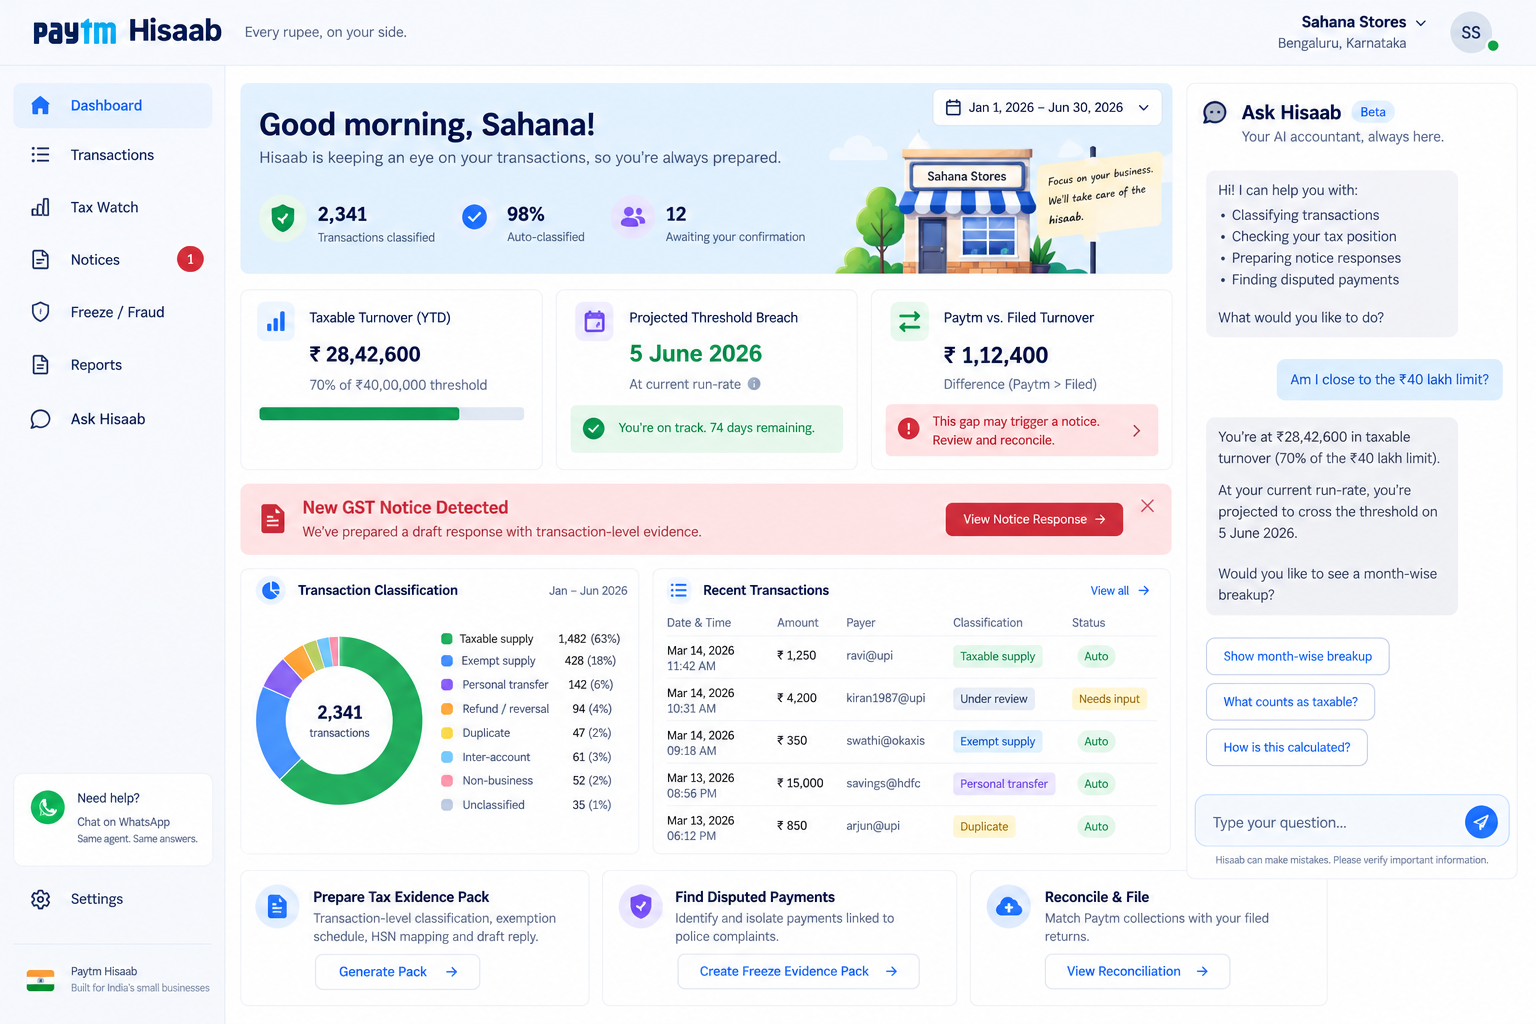
\includegraphics[width=\textwidth,height=0.70\textheight,keepaspectratio]{Paytm-Hisaab_website_look.png}
\end{center}
\vspace{0.1cm}
\hspace{0.05cm}{\scriptsize\color{muted}One surface: what every payment was classified as, how close she is to the threshold, and the packs. The same agent runs on WhatsApp, where she actually is.}
\note{{\color{navy}\bfseries\normalsize 8.~What the merchant sees}\par\vspace{0.55em}\textbf{0:20 --- a glance slide. Do not tour the UI.}
\\[0.4em]
One sentence: everything classified, how close she is to the threshold, and the
packs, on one surface.
\\[0.4em]
Then the WhatsApp point --- the same agent, where she actually is --- and advance.
\\[0.4em]
If someone asks whether this is built: the chat and the tools are live; this
screen is the product surface we are designing toward.}
\end{frame}

% ============================================================ 9. ARCHITECTURE
\begin{frame}{Built on Phinite}{Two agent graphs, four agents, ten deterministic skills}
\vspace{0.15cm}
\begin{columns}[T]
\begin{column}{0.53\textwidth}
{\scriptsize
\begin{tabular}{@{}L{1.75cm}L{4.7cm}@{}}
\multicolumn{2}{@{}l}{\color{navy}\bfseries\small hisaab-watch \;\scriptsize(autonomous: cron + API)}\\
\midrule
Provenance & proposes a tag and a reason for the hard credits \\
Evidence   & assembles packs: freeze evidence, then exemption schedules and HSN \\
\addlinespace[0.6em]
\multicolumn{2}{@{}l}{\color{navy}\bfseries\small hisaab-merchant \;\scriptsize(conversational: chat)}\\
\midrule
Merchant   & the conversation: attestation, alerts, Kannada \\
Escalation & decides when to stop and route to a human CA \\
\bottomrule
\end{tabular}}
\\[0.75em]
{\scriptsize\color{muted}The nightly pass writes its queue to the ledger; the chat reads it when she opens it. Deliberately \emph{not} a graph-to-graph call: a queue that outlives either run is what makes the handoff robust.}
\end{column}
\begin{column}{0.44\textwidth}
\card{5.7cm}{{\bfseries\color{navy}Permissions are the product}\\[0.4em]
\scriptsize Provenance proposes, \red{never commits}.\\[0.25em]
\scriptsize Merchant is the \emph{only} agent that can commit a tag.\\[0.25em]
\scriptsize Evidence is \red{read-only}. It cannot edit a classification to make a pack look better.\\[0.25em]
\scriptsize Escalation can \red{halt} any pack; a human approves.}
\\[0.5em]
\hspace{0.1cm}\begin{minipage}{5.7cm}{\scriptsize\color{muted}Ten tools run live against a hosted service. Every number in a pack traces back, in the trace, to the credit and the attestation behind it.}\end{minipage}
\end{column}
\end{columns}
\note{{\color{navy}\bfseries\normalsize 9.~Built on Phinite}\par\vspace{0.55em}\textbf{0:40 --- for the technical judges.}
\\[0.4em]
Two agent graphs, not four loose agents: \texttt{hisaab-watch} runs autonomously on
cron, \texttt{hisaab-merchant} is the conversation. The nightly pass writes a queue;
the chat reads it when she opens it --- deliberately not a graph-to-graph call,
because a queue that outlives either run is what makes the handoff robust.
\\[0.4em]
\textbf{Spend your time on the right-hand card.} The strongest line in it:
the Evidence agent is read-only --- \emph{the agent that builds the defence cannot
edit the evidence.} And only the Merchant agent can commit an attested tag.
\\[0.4em]
Those are enforced as Phinite tool policies, not conventions, and a denied call
shows up in the trace.}
\end{frame}

% ============================================================ 10. DESIGN DECISIONS
\begin{frame}{Four decisions that make it defensible}
\vspace{0.3cm}
\begin{columns}[T]
\begin{column}{0.48\textwidth}
\card{6.0cm}{{\bfseries\color{navy}1. Arithmetic lives in skills, not the model}\\[0.35em]
\scriptsize Turnover, projections and apportionment are deterministic Python: versioned, testable, traceable. Wrapping arithmetic in an LLM is the standard tell, and the trace would show it.}
\\[0.35em]
\card{6.0cm}{{\bfseries\color{navy}3. Refusing to guess is a feature}\\[0.35em]
\scriptsize An \texttt{unclassified} credit routed to the merchant costs one tap. A confident wrong tag inside an evidence pack is a catastrophe. We report the refusal rate honestly.}
\end{column}
\begin{column}{0.48\textwidth}
\card{6.0cm}{{\bfseries\color{navy}2. Attestation is the promotion boundary}\\[0.35em]
\scriptsize Nothing enters a production pack that the merchant has not confirmed. Sandbox to UAT to prod, with her tap as the gate.}
\\[0.35em]
\card{6.0cm}{{\bfseries\color{navy}4. Ground truth, so accuracy is a number}\\[0.35em]
\scriptsize We simulated a year of a shop's life from a known process, split into what Paytm can see and what really happened. Agents read only the visible half, which is why we quote error bars instead of vibes.}
\end{column}
\end{columns}
\note{{\color{navy}\bfseries\normalsize 10.~Four decisions}\par\vspace{0.55em}\textbf{0:35 --- the slide that separates you from a demo.}
\\[0.4em]
Lead with \#1: all arithmetic is deterministic Python, not model output. Wrapping
arithmetic in an LLM is the standard tell, and the trace would show it.
\\[0.4em]
Then \#3: refusing to guess is a feature. An \texttt{unclassified} credit costs one
tap; a confident wrong tag inside an evidence pack is a catastrophe.
\\[0.4em]
Skim \#2 and \#4 --- one clause each. \#4 is worth a beat if the room is technical:
we generated ground truth, so accuracy is a number instead of a claim.}
\end{frame}

% ============================================================ 11. DEMO / ATTESTATION
\begin{frame}{Demo $\cdot$ Sahana Stores, Jayanagar}{An ordinary Tuesday, before anything goes wrong}
\vspace{0.1cm}
\begin{columns}[T]
\begin{column}{0.48\textwidth}
{\scriptsize\color{muted}Tuesday 10 March. Thirty-nine credits came in over the weekend. The agent asks about \hi{three}.}
\\[0.4em]
\card{5.9cm}{{\kn\scriptsize ಭಾನುವಾರ ರಾತ್ರಿ ₹15,000. ನಿಮ್ಮ ಸ್ವಂತ ಹಣವೇ?}\\[0.25em]
{\color{muted}\scriptsize \qm{₹15,000 at 11:04pm Sunday, from your savings account. Your own money?}}\\[0.35em]
{\scriptsize\color{navy}\fbox{\kn ಹೌದು}\;\fbox{\kn ಇಲ್ಲ}}}
\\[0.4em]
{\scriptsize $\cdot$\; ₹7,500 from her husband, scanned at the shop QR\\[0.25em]
$\cdot$\; ₹4,850 from Raghu Shetty, who has bought twice before. A real sale, and the agent \emph{asks} rather than assumes.}
\\[0.4em]
{\scriptsize\color{muted}The other thirty-six settle silently, and a ₹23 payment nobody can place is left alone.}
\end{column}
\begin{column}{0.48\textwidth}
\ocard{amber}{6.1cm}{{\bfseries\color{amber}And yes, two of those three should not be there}\\[0.35em]
\scriptsize A business QR is not for personal money, and the terms say so. It arrives anyway: family, own top-ups, a chit payout. The rule does not prevent it. It only means \emph{nobody keeps a record of it.}}
\\[0.45em]
{\scriptsize Paytm already reads the signals: channel, linked VPAs, payer history. What no system has is the \hi{merchant's own answer}, given at the time, in her language, and kept.}
\\[0.45em]
{\scriptsize That record is what the next two slides are built from: first for the police, then for the department.}
\end{column}
\end{columns}
\note{{\color{navy}\bfseries\normalsize 11.~Demo --- an ordinary Tuesday (beat 1)}\par\vspace{0.55em}\textbf{0:45 --- or hand over to the live demo here.}
\\[0.4em]
Thirty-nine credits came in over the weekend, the agent asks about \textbf{three}.
Read the Kannada line if you can; otherwise read the gloss under it.
\\[0.4em]
\textbf{Do not hide from the right-hand card --- lead with it.} The mid-review
point was that personal money is not allowed on a business QR. Correct, and we say
so on the slide. The argument is that the rule does not stop it, it only means no
one records it, and an unrecorded credit is what an authority later reads as income.
\\[0.4em]
\textbf{Second half of that card matters just as much.} We are not claiming Paytm
does nothing. It already reads channel, linked VPAs and payer history. What no
system has is her own answer, captured while it is still knowable. That is the
product, and it is a smaller, truer claim than the one we started with.
\\[0.4em]
\textbf{Before going on stage:} confirm the attestation queue is whole ---
\texttt{pending\_total} must be 3. A rehearsal that taps through this beat spends the
queue, and Render needs a clear-cache redeploy to restore it.}
\end{frame}

% ============================================================ 12. DEMO / THE FREEZE
\begin{frame}{Demo $\cdot$ The emergency}{The account is frozen at 09:30 and the supplier payment is due}
\vspace{0.2cm}
\begin{columns}[T]
\begin{column}{0.46\textwidth}
{\scriptsize She sold someone 12kg of onions. That customer was three layers downstream of a fraud victim. She is not named in the FIR, which was filed in another state, and \hi{339 payments} came in that week.}
\\[0.5em]
\card{5.8cm}{{\bfseries\color{navy}The agent isolates it}\\[0.35em]
\scriptsize ₹4,200 on 21 March at 19:47, till POS01. Matched by UTR \emph{and independently} by amount and date.\\[0.3em]
\scriptsize The sale record comes with it: the POS bill, the items, the till and the minute.}
\end{column}
\begin{column}{0.49\textwidth}
\ocard{amber}{6.1cm}{{\bfseries\color{amber}And the decoy it did not choose}\\[0.35em]
\scriptsize A \emph{second} ₹4,200 that same week, from a regular customer. Listed in the pack, and explicitly \emph{not} named as the disputed one. Only the date separates them.}
\\[0.5em]
{\scriptsize Then it drafts the NCRP-CFCFRMS grievance, citing the judgments that only the \emph{disputed amount} should be lien-marked, not the whole account.}
\\[0.5em]
{\scriptsize\color{bad}\bfseries It never asserts that she is innocent.}\\[0.1em]
{\scriptsize\color{muted}Some frozen accounts genuinely are mule accounts. The agent assembles evidence; a human decides. Escalation holds the pack for approval.}
\end{column}
\end{columns}
\note{{\color{navy}\bfseries\normalsize 12.~Demo --- the emergency (beat 4)}\par\vspace{0.55em}\textbf{0:50 --- this is now the lead case. Give it the most time of the three.}
\\[0.4em]
Set the stakes in one sentence: account frozen at half nine, supplier payment due,
339 payments came in that week, and she is not named in the FIR.
\\[0.4em]
\textbf{Why this one leads.} She did nothing wrong and there is no rule she broke.
She sold onions to a customer who turned out to be laundering. Every objection
available against the tax case --- she should not have taken personal money on that
QR, she should have registered --- has no purchase here at all.
\\[0.4em]
The agent isolates ₹4,200 by UTR \emph{and independently} by amount and date, and
brings the POS bill with it --- the items, till POS01, 19:47.
\\[0.4em]
\textbf{The decoy is the point.} A second ₹4,200 that same week from a regular
customer, listed in the pack and explicitly not chosen. Anyone can match an amount;
the pack shows its work.
\\[0.4em]
Finish on the red line: it never asserts she is innocent. Some frozen accounts
genuinely are mule accounts. We assemble evidence; a human decides, and Escalation
holds the pack for approval.}
\end{frame}

% ============================================================ 13. DEMO / TAX
\begin{frame}{Demo $\cdot$ The warning, and the notice}{The same ledger, read for the other authority}
\vspace{0.15cm}
\begin{columns}[T]
\begin{column}{0.38\textwidth}
{\scriptsize\color{muted}Replayed as of 31 January:}
\\[0.35em]
\ocard{good}{4.8cm}{{\bfseries\color{ink}\scriptsize\qm{At your current rate you cross ₹40 lakh around {\color{bad}14 March}. You will need to register.}}\\[0.35em]
{\scriptsize\color{muted}\grn{43 days of warning}, and the date is computed, not typed.}}
\\[0.45em]
{\scriptsize\color{bad}\bfseries This beat is what makes the pitch safe.}\\[0.1em]
{\scriptsize\color{muted}Its first act on the tax side is telling her to register.}
\end{column}
\begin{column}{0.58\textwidth}
{\scriptsize\color{muted}Then the notice arrives, claiming {\color{bad}\bfseries ₹60.98L} of turnover:}
\\[0.3em]
{\scriptsize
\begin{tabular}{@{}lr@{\hskip 1.2em}l@{}}
\multicolumn{2}{@{}l}{\color{navy}\bfseries Aggregate turnover \quad ₹42.2L} & \sub{within \grn{1.6\%} of truth} \\
\midrule
Exempt supplies      & ₹31.3L & \sub{vegetables, loose rice} \\
Taxable supplies     & ₹10.9L & \sub{branded goods, oil, soap} \\
\addlinespace[0.45em]
\multicolumn{2}{@{}l}{\color{navy}\bfseries Not turnover at all \quad ₹18.8L} & \sub{every line traced} \\
\midrule
Her own accounts     & ₹7.4L & \sub{top-ups before supplier runs} \\
Family               & ₹6.1L & \sub{spouse, parent, in-law} \\
Loans, chit, gifts   & ₹4.3L & \sub{chit payout, festival gifts} \\
Refunds, duplicates  & ₹1.0L & \sub{crate returns, double-taps} \\
\bottomrule
\end{tabular}}
\\[0.45em]
{\scriptsize And it says plainly: \hi{the claim is wrong, and you \emph{did} cross ₹40 lakh on 14 March. You must register.}}
\end{column}
\end{columns}
\note{{\color{navy}\bfseries\normalsize 13.~Demo --- the warning and the notice (beats 2 and 3)}\par\vspace{0.55em}\textbf{0:50 --- two tax beats on one slide, deliberately compressed.}
\\[0.4em]
Left: replayed as of 31 January, the agent says she crosses ₹40 lakh around
14 March. \textbf{Say the red line out loud} --- its first act on the tax side is
telling her she owes a registration. That is what stops the room turning hostile.
\\[0.4em]
Right: the notice claims ₹60.98 lakh, and the pack answers it line by line, every
figure traceable to transaction IDs. Then the honest half:
\textbf{the claim is wrong, and she did cross ₹40 lakh, and she must register.}
\\[0.4em]
\textbf{If a judge diffs this against slide 5:} slide 5 shows seeded truth
(₹42.9L), this shows what our system computed (₹42.2L). The 1.6\% between them
\emph{is} the accuracy claim --- say that, do not hedge.
\\[0.4em]
\textbf{If pushed on the personal and own-account lines:} same answer as slide 11.
Those credits should not be on a business QR, they are there anyway, and the
alternative to classifying them is letting them be read as income.}
\end{frame}

% ============================================================ 14. NUMBERS
\begin{frame}{What we can actually prove}{One merchant, one year, 13,267 credits, scored against seeded truth}
\vspace{0.45cm}
\begin{columns}[T]
\begin{column}{0.33\textwidth}
\begin{center}\bignum{1.6\%}{error on aggregate turnover\\ (taxable share within 1\%)}\end{center}
\vspace{0.55cm}
\begin{center}\bignum{43 days}{of warning before the\\ threshold crossing}\end{center}
\end{column}
\begin{column}{0.33\textwidth}
\begin{center}\bignum{1.3 a day}{median questions asked.\\ 189 in a year, never over 3}\end{center}
\vspace{0.55cm}
\begin{center}\bignum{zero}{credits left untagged\\ across the whole year}\end{center}
\end{column}
\begin{column}{0.30\textwidth}
\card{3.8cm}{{\bfseries\color{navy}The honest baseline}\\[0.35em]
\scriptsize A 50-line rules-only classifier gets 99.3\% on sale vs not-a-sale, but catches only \red{77.8\%} of non-sale credits.\\[0.3em]
\scriptsize That residue alone puts two eval merchants on the \emph{wrong side} of ₹40L.\\[0.3em]
\scriptsize Closing it is what the agent plus one tap is for.}
\end{column}
\end{columns}
\vspace{0.45cm}
\hspace{0.1cm}{\scriptsize\color{muted}She corrected the agent 52 times that year. Those corrections are the ledger's strongest evidence, not its failures.}
\note{{\color{navy}\bfseries\normalsize 14.~What we can actually prove}\par\vspace{0.55em}\textbf{0:30 --- do not read all four. Pick two.}
\\[0.4em]
Lead with \textbf{1.6\%} error on turnover and \textbf{1.3 questions a day}. The
other two are there to be read, not narrated.
\\[0.4em]
\textbf{The credibility move is the box on the right} --- volunteer the weakness
before anyone finds it. A rules-only baseline gets 99.3\% on sale vs not-a-sale
but catches only 77.8\% of non-sale credits, and that residue alone puts two eval
merchants on the wrong side of ₹40 lakh. Closing it is what the agent plus one tap is for.
\\[0.4em]
Last line if you have the beat: she corrected the agent 52 times that year, and
those corrections are the ledger's strongest evidence, not its failures.}
\end{frame}

% ============================================================ 15. CLOSE
\begin{frame}{The line we do not cross}{Accuracy, not minimisation}
\vspace{0.3cm}
\begin{columns}[T]
\begin{column}{0.52\textwidth}
{\scriptsize
$\cdot$\; We \hi{never assert innocence} on a freeze. Some accounts really are mule accounts. We assemble evidence; a human decides.\\[0.5em]
$\cdot$\; We \hi{file nothing} with any authority. Artefacts only; the merchant or their CA files.\\[0.5em]
$\cdot$\; We compute what she \hi{genuinely owes} and say so plainly, including \qm{you crossed the threshold, you must register.}\\[0.5em]
$\cdot$\; We \hi{never assert a final liability}. We compute, show the workings, and route to a CA.\\[0.5em]
$\cdot$\; A business QR is \hi{not for personal money}. We do not excuse it. We record it, so it is not read as income.}
\end{column}
\begin{column}{0.44\textwidth}
\begin{tikzpicture}\node[rounded corners=4pt,fill=navy,text=white,inner sep=10pt,text width=5.7cm,align=left]{
{\bfseries Why this has to be Paytm}\\[0.45em]
\scriptsize The rail is the only place provenance is cheap. Everyone else arrives eighteen months late, when the answer is already unrecoverable.\\[0.45em]
\scriptsize A frozen merchant cannot transact at all: dead Soundbox and zero GMV the same morning, before it becomes the sign on the shutter, \emph{\qm{No UPI. Cash only.}}
};\end{tikzpicture}
\end{column}
\end{columns}
\vspace{0.4cm}
\begin{center}
{\large\color{navy}\bfseries Paytm Hisaab}\quad{\color{muted}every rupee, on your side.}
\end{center}
\note{{\color{navy}\bfseries\normalsize 15.~The line we do not cross}\par\vspace{0.55em}\textbf{0:30 --- the non-negotiables, fast, then land.}
\\[0.4em]
Run the five bullets at pace. The one to hit is the first: we never assert
innocence on a freeze. The last is the mid-review answer, on the slide on purpose.
\\[0.4em]
Then the navy box: provenance is cheap only on the rail, and a frozen merchant
stops transacting the same morning.
\\[0.4em]
Final line, unhurried: \emph{``Paytm Hisaab. Every rupee, on your side.''} Stop talking.
\\[0.5em]
{\scriptsize
{\color{navy}\bfseries --- Q\&A prep ---}
\\[0.3em]
\textbf{``Merchants may not take personal money on a business QR.''} Correct, and
slide 11 says so before you have to. It arrives anyway, and the alternative to
recording it is letting an authority read it as income. We are not defending the
behaviour --- we are refusing to let it become a liability.
\\[0.3em]
\textbf{``Paytm already tags transactions.''} It does, and we build on that rather
than around it: channel, linked VPAs and payer history feed the rules layer. What
no tag carries is her attestation --- the part an authority accepts, and the only
part she alone can give.
\\[0.3em]
\textbf{``No return mismatch?''} That check needs a \emph{registered} composition
dealer who filed a CMP-08 to disagree with. Ours is unregistered, which is why she
gets a notice at all; the eval split has one with four quarters seeded.
\\[0.3em]
\textbf{``Exempt vs taxable on a QR sale?''} Not per payment. We apportion by value
from that shop's own POS-billed ratio and label it an estimate. Labelling each sale
by its majority side understated taxable turnover threefold.
\\[0.3em]
\textbf{``Four LLM calls in a trenchcoat?''} Everything deterministic is a skill and
four agents is the ceiling. If twenty lines of Python replaces an agent, it should
have been a skill --- the trace shows which is which.
\\[0.3em]
\textbf{``No standing with the police.''} Agreed: Paytm supplies, the merchant
files. By design. Cash sales are real, out of scope, and on the slide.}}
\end{frame}

\end{document}
"
\ifdefined\shownotes
  \setbeamertemplate{note page}{%
    \usebeamercolor[fg]{normal text}%
    \vspace{0.2em}%
    {\scriptsize\color{muted}Paytm Hisaab \;$\cdot$\; speaker notes}\hfill
    {\scriptsize\color{muted}slide \insertframenumber\ of 15}\par
    \vspace{0.25em}{\color{ptmcyan}\rule{\textwidth}{1.5pt}}\par
    \vspace{0.55em}\footnotesize\raggedright\insertnote\par}
  \setbeameroption{show only notes}
\fi

\begin{document}

% ============================================================ 1. TITLE
{\setbeamertemplate{footline}{}
\begin{frame}[plain]
\vspace{0.9cm}
\begin{center}
{\fontsize{38}{42}\selectfont\bfseries\color{navy}Paytm\;\color{ink}Hisaab}\\[0.45em]
{\Large\color{muted}Every rupee, on your side.}\\[0.9em]
{\color{ptmcyan}\rule{2.8cm}{2.5pt}}\\[0.9em]
{\large\color{ink}The agent that lets a merchant account for their own money}\\[0.15em]
{\large\color{ink}when someone in authority demands an explanation.}\\[1.3em]
{\small\color{muted}Agent Labs Buildathon \;$\cdot$\; Phinite $\times$ Paytm \;$\cdot$\; Track 2: AI for Small Businesses}
\end{center}
\note{{\color{navy}\bfseries\normalsize 1.~Title}\par\vspace{0.55em}\textbf{0:10 --- open cold.} Do not read the title or the tagline off the slide.
\\[0.4em]
Say: \emph{``I want to tell you about a man in Haveri who opened an envelope.''} Then advance.
\\[0.4em]
Nothing on this slide needs explaining. The tagline lands at the end, not here.}
\end{frame}}

% ============================================================ 2. STORY
\begin{frame}{Haveri, 2025}{A vegetable vendor opens an envelope}
\vspace{0.05cm}
\begin{columns}[T]
\begin{column}{0.52\textwidth}
\vspace{0.15cm}
He sells vegetables. Vegetables are \hi{exempt} from GST.\\[0.6em]
He also took UPI, because Paytm asked him to.\\[0.6em]
Four years of credits into his account, added up and billed as income:
\begin{center}\vspace{0.1em}{\fontsize{30}{32}\selectfont\bfseries\color{bad}₹29 lakh}\end{center}
\end{column}
\begin{column}{0.44\textwidth}
\ocard{hairline}{5.4cm}{\centering
  {\color{muted}\scriptsize Within weeks, on shutters across Karnataka:}\\[0.6em]
  {\fontsize{20}{23}\selectfont\bfseries\color{ink}\qm{No UPI.\\ Cash only.}}\\[0.6em]
  {\color{muted}\scriptsize A statewide boycott, by the merchants who had just adopted it.}}
\end{column}
\end{columns}
\vspace{0.25cm}
\hspace{0.1cm}{\small\sub{Withdrawn for the traders who could \emph{show} what they sold. Most could not. And tax is no longer the only authority asking.}}
\note{{\color{navy}\bfseries\normalsize 2.~Haveri, 2025}\par\vspace{0.55em}\textbf{0:45 --- the hook. Tell it, do not summarise it.}
\\[0.4em]
Four beats, in this order: he sells vegetables; vegetables are exempt from GST;
he took UPI because \emph{we} asked him to; the department added up four years of
credits and sent him a bill for \textbf{₹29 lakh}.
\\[0.4em]
\textbf{Pause on the number.} Then the card: within weeks, shutters across Karnataka
read ``No UPI, cash only.'' Merchants we had just onboarded, boycotting the rail.
\\[0.4em]
Close on the bottom line --- the notices were withdrawn for traders who could
\emph{show} what they sold. Most could not. That verb is the whole product.
\\[0.4em]
\textbf{Then the bridge:} \emph{``and tax is no longer the only authority asking.''}
That sentence is doing the repositioning --- Haveri is not a tax story here, it is
the moment taking digital money became a liability. The sharper version of it is
two slides away.
\\[0.4em]
\textbf{Do not say this is happening right now.} It is 2025. The next slide is
what makes it current, and a judge who knows the episode will respect the distinction.}
\end{frame}

% ============================================================ 3. STILL HAPPENING
\begin{frame}{And this is not a 2025 story}{CAclubindia, last updated 02 September 2026: ten days ago}
\vspace{0.1cm}
\begin{center}

\includegraphics[width=12.4cm]{gst-notices-2026.png}
\end{center}
\vspace{0.35cm}
\card{13.1cm}{\scriptsize\qm{During August 2026, the GST Department issued a significant number of notices covering different financial years and involving a wide range of issues\ldots\ They covered matters such as ITC mismatches, ineligible credit, \hi{differences in turnover}, wrong GST classification or rate, \hi{exemption claims}, Reverse Charge Mechanism\ldots}}
\vspace{0.3cm}

\hspace{0.1cm}{\small Those two categories are the whole content of an evidence pack. And this is the \emph{slower} of the two authorities. The other one freezes the account first.}
\note{{\color{navy}\bfseries\normalsize 3.~And this is not a 2025 story}\par\vspace{0.55em}\textbf{0:25 --- fast. This slide exists to kill one objection.}
\\[0.4em]
Say: \emph{``That was last year. This was published ten days ago.''}
\\[0.4em]
Do not read the quote. Point at the two bolded phrases only ---
\textbf{differences in turnover} and \textbf{exemption claims} --- and say those
two categories are the entire content of what we build.
\\[0.4em]
\textbf{Land on the last line and move.} It is the handoff into the police
slide: this is the slower authority. The other one freezes first and asks
afterwards. Do not linger here --- tax is no longer the headline.}
\end{frame}

% ============================================================ 4. THE TRAP
\begin{frame}{Every rupee a merchant receives is now evidence}{Today it is only ever used against them}
\vspace{0.05cm}
\begin{columns}[T]
\begin{column}{0.47\textwidth}
\ocard{bad}{6.0cm}{{\bfseries\color{bad}The cyber-crime police}\\[0.35em]
\scriptsize Fraud money layers through accounts within minutes. The shop at the end of the chain, the one that sold someone a watermelon, is frozen. It did nothing wrong, is not named in the FIR, and finds out when a payment declines.}
\end{column}
\begin{column}{0.47\textwidth}
\card{6.1cm}{{\bfseries\color{navy}The tax department}\\[0.35em]
\scriptsize Compares UPI collections against filed returns and bills the difference. Registered traders too, with QR, wallet, card and cash deposits all in scope.}
\end{column}
\end{columns}
\vspace{0.4cm}
\begin{center}
{\large Both demand the same artefact: \hi{what was each rupee, actually?}}\\[0.3em]
{\small\color{muted}Paytm already sees more of this than anyone. What is missing is the \emph{merchant's own answer}, captured when it is still knowable.}
\end{center}
\vspace{0.15cm}
{\color{hairline}\hrule height 1pt}
\vspace{0.35em}
\hspace{0.05cm}{\scriptsize\bfseries\color{bad}What it costs Paytm:}~{\scriptsize a frozen merchant stops transacting that morning. A frightened one takes the QR down for good. Dead Soundbox, zero GMV, no lending origination.}
\note{{\color{navy}\bfseries\normalsize 4.~Every rupee is now evidence}\par\vspace{0.55em}\textbf{0:40 --- two authorities, one unanswerable question.}
\\[0.4em]
\textbf{Left card first and give it the time.} Fraud money layers within minutes,
and the shop at the end of the chain, \emph{the one that sold someone a watermelon},
gets frozen. It did nothing wrong, it is not named in the FIR, and it finds out
when a payment declines. Use the watermelon.
\\[0.4em]
Right card briskly: the department reconciles collections against filed returns
and bills the difference. One sentence, then move.
\\[0.4em]
Then the pivot: both demand the same artefact --- what was each rupee, actually.
\\[0.4em]
\textbf{Say the grey line as written.} We do \emph{not} claim Paytm does nothing
with this data --- it tags plenty. The gap is the merchant's own answer, captured
when it is still knowable. Claiming otherwise in this room gets corrected.
\\[0.4em]
\textbf{Slow down for the red line.} This is the business case, not a footnote:
a frozen merchant stops transacting that morning, a frightened one takes the QR
down for good. Dead Soundbox, zero GMV, no lending origination.}
\end{frame}

% ============================================================ 5. THE BAR
\begin{frame}{Gross credits are not turnover}{One shop, one year, ₹60.98 lakh of credits}
\vspace{0.1cm}
\begin{center}
\begin{tikzpicture}[x=1cm,y=1cm]
% --- what the notice counts
\node[anchor=west,font=\scriptsize\bfseries,text=bad] at (-0.05,1.80) {WHAT THE NOTICE COUNTS AS TURNOVER};
\fill[bad!85,rounded corners=2pt] (0,1.06) rectangle (11.4,1.60);
\node[font=\small\bfseries,text=white] at (5.7,1.33) {₹60.98 lakh};

% --- what actually happened   (1 lakh = 0.18696 cm, so the bars are the same length)
\node[anchor=west,font=\scriptsize\bfseries,text=navy] at (-0.05,0.66) {WHAT ACTUALLY HAPPENED};
\fill[good!80,rounded corners=2pt]  (0,-0.08)     rectangle (6.001,0.46);
\fill[good!45]                      (6.001,-0.08) rectangle (8.002,0.46);
\fill[ptmcyan!70]                   (8.002,-0.08) rectangle (9.385,0.46);
\fill[navy!55]                      (9.385,-0.08) rectangle (10.451,0.46);
\fill[amber!70]                     (10.451,-0.08)rectangle (11.255,0.46);
\fill[muted!60,rounded corners=2pt] (11.255,-0.08)rectangle (11.4,0.46);

% brackets
\draw[navy,line width=0.8pt] (0,-0.22) -- (0,-0.36) -- (8.002,-0.36) -- (8.002,-0.22);
\node[anchor=north,font=\scriptsize,text=navy,align=center] at (4.0,-0.38)
  {\bfseries ₹42.9L aggregate turnover\quad{\color{muted}\scriptsize exempt ₹32.1L + taxable ₹10.7L}};
\draw[bad,line width=0.8pt] (8.002,-0.22) -- (8.002,-0.36) -- (11.4,-0.36) -- (11.4,-0.22);
\node[anchor=north,font=\scriptsize,text=bad,align=center] at (9.7,-0.38)
  {\bfseries ₹18.1L that is not turnover at all};

% legend
\node[font=\scriptsize,text=ink] at (5.7,-1.02) {%
\textcolor{good!80}{$\blacksquare$}~Exempt sales \quad
\textcolor{good!45}{$\blacksquare$}~Taxable sales \quad
\textcolor{ptmcyan!70}{$\blacksquare$}~Her own accounts ₹7.4L};
\node[font=\scriptsize,text=ink] at (5.7,-1.40) {%
\textcolor{navy!55}{$\blacksquare$}~Family ₹5.7L \quad
\textcolor{amber!70}{$\blacksquare$}~Loans, chit, gifts ₹4.3L \quad
\textcolor{muted!60}{$\blacksquare$}~Refunds \& duplicates ₹0.7L};
\end{tikzpicture}
\end{center}
\vspace{0.15cm}
\hspace{0.1cm}{\small\sub{Personal money does not belong on a business QR. It arrives anyway, reads as turnover, and hides the one credit the police will ask about.}}
\note{{\color{navy}\bfseries\normalsize 5.~Gross credits are not turnover}\par\vspace{0.55em}\textbf{0:45 --- the hinge of the pitch. Let the picture work.}
\\[0.4em]
Say: \emph{``One shop, one year, ₹60.98 lakh of credits. The red bar is what the
notice counts as turnover --- all of it.''}
\\[0.4em]
Then the bottom bar. \textbf{Stop talking for two seconds} and let them read it.
\\[0.4em]
₹42.9L really is turnover, and we say so. ₹18.1L is not: her savings account, her
husband, a chit payout, a double-tap on the Soundbox.
\\[0.4em]
\textbf{Get in front of the obvious objection.} Personal money is not supposed to
touch a business QR. Say so first, then say it arrives anyway --- that is an
observation about merchants, not a loophole we are selling. The rule does not stop
it; it only means no one is keeping a record of it.
\\[0.4em]
\textbf{And close on the second use.} This volume is also why she cannot find the
one credit the police care about. Same bar, same problem, and the freeze slide
pays it off.
\\[0.4em]
If challenged on the numbers: seeded ground truth from our generator, not an
estimate. Accuracy against it is slide 14.}
\end{frame}

% ============================================================ 6. INSIGHT
\begin{frame}{The insight}{Most teams would build the tax tool \emph{or} the fraud tool. They are the same engine.}
\vspace{0.15cm}
\begin{center}
\begin{tikzpicture}[font=\scriptsize]
\node[rounded corners=4pt,fill=navy,text=white,inner sep=7pt,align=center,text width=3.5cm]
  (eng) {\bfseries\small Provenance Ledger\\[0.15em] a merchant-attested label on every incoming credit};
\node[rounded corners=4pt,fill=tint,draw=bad,inner sep=6pt,align=center,text width=4.0cm]
  (tax) at ($(eng.east)+(3.7,0.78)$) {\bfseries The disputed rupee\\ freeze pack, NCRP grievance};
\node[rounded corners=4pt,fill=tint,draw=hairline,inner sep=6pt,align=center,text width=4.0cm]
  (fra) at ($(eng.east)+(3.7,-0.78)$) {\bfseries Defensible turnover\\ threshold watch, notice pack};
\draw[-{Stealth[length=2.5mm]},ptmcyan,line width=1.3pt] (eng.east) -- ++(0.5,0) |- (tax.west);
\draw[-{Stealth[length=2.5mm]},ptmcyan,line width=1.3pt] (eng.east) -- ++(0.5,0) |- (fra.west);
\node[anchor=east,text width=2.9cm,align=right,text=muted] at ($(eng.west)+(-0.35,0)$)
  {Both are downstream \emph{reads} of one ledger. Two output formats, not two products.};
\end{tikzpicture}
\end{center}
\vspace{0.1cm}
\begin{center}
\begin{tikzpicture}\node[rounded corners=4pt,fill=tint,inner sep=8pt,text width=11.2cm,align=center]{
{\bfseries\color{navy}The wedge nobody else has.}\\[0.25em]
\small Khatabook and Vyapar keep books after the fact. ClearTax files after the fact.\\
Neither sits on the rail \emph{at the moment money moves}. Paytm does.\\[0.25em]
\small Classification is cheap at the instant of the transaction,\\ and unrecoverable eighteen months later.
};\end{tikzpicture}
\end{center}
\note{{\color{navy}\bfseries\normalsize 6.~The insight}\par\vspace{0.55em}\textbf{0:40 --- why this is one product, not two.}
\\[0.4em]
Say: \emph{``Most teams would build the fraud tool or the tax tool. They are the
same engine.''} Both are downstream reads of one ledger --- two output formats,
and the freeze pack is the one we lead with.
\\[0.4em]
Then the wedge, and say it slowly because it is the defensible-moat answer:
Khatabook and Vyapar keep books after the fact, ClearTax files after the fact.
Neither sits on the rail at the moment money moves. \textbf{Paytm does.}
\\[0.4em]
Landing line: classification is cheap and accurate at the instant of the
transaction, and unrecoverable eighteen months later when the notice arrives.}
\end{frame}

% ============================================================ 7. THE ENGINE
\begin{frame}{The engine}{Eight tags, one tap}
\vspace{0.15cm}
\begin{columns}[T]
\begin{column}{0.45\textwidth}
{\color{navy}\bfseries\small Every incoming credit gets one tag}\\[0.4em]
{\scriptsize
\begin{tabular}{@{}ll@{}}
\texttt{taxable\_supply}    & ordinary sale \\
\texttt{exempt\_supply}     & vegetables, milk, loose rice \\
\texttt{personal\_transfer} & spouse, parent, sibling \\
\texttt{inter\_account}     & her own money \\
\texttt{refund\_reversal}   & money back from a vendor \\
\texttt{duplicate}          & paid twice, one refunded \\
\texttt{non\_business}      & loan, chit payout, gift \\
{\color{bad}\texttt{unclassified}} & {\color{bad}not enough signal: ask her} \\
\end{tabular}}
\\[0.75em]
{\scriptsize\color{muted}98.6\% are ordinary sales, settled by rules. The agent reasons only about the 1.4\% that need judgement.}
\end{column}
\begin{column}{0.51\textwidth}
\card{6.6cm}{{\bfseries\color{navy}The agent proposes. The merchant attests.}\\[0.4em]
\scriptsize You cannot infer \qm{my husband sent this} from a QR payment. The agent proposes a tag \emph{with its reason}; she confirms with one tap, in Kannada, batched daily.\\[0.45em]
\scriptsize Not a fallback. A ledger she attested \emph{at the time} survives a hearing. An algorithm's guess, made under duress a year later, does not.}
\\[0.55em]
\hspace{0.15cm}\begin{minipage}{6.6cm}
{\bfseries\color{navy}\small Budget: at most 3 questions a day.}\\[0.15em]
{\scriptsize\color{muted}Over a simulated year: \hi{189 questions, median 1.3 a day}. Ask more and the product is dead.}
\end{minipage}
\end{column}
\end{columns}
\note{{\color{navy}\bfseries\normalsize 7.~The engine}\par\vspace{0.55em}\textbf{0:45 --- the mechanism. Do not read the tag list.}
\\[0.4em]
Gesture at the eight tags, say ``eight labels, every incoming credit gets one,''
and move to the right-hand card, which is the real content.
\\[0.4em]
\textbf{The line that matters:} you cannot infer ``my husband sent this'' from a
QR payment. So the agent proposes a tag \emph{with its reason} and she confirms
with one tap. This is not a fallback --- a ledger she attested contemporaneously
survives a hearing; an algorithm's guess produced under duress a year later does not.
\\[0.4em]
Then the budget: at most three questions a day, and we measured 189 across a
year, median 1.3. Ask more than that and the product is dead.
\\[0.4em]
If asked about cost: 98.6\% are ordinary sales settled by rules. The model only
sees the 1.4\% that need judgement.}
\end{frame}

% ============================================================ 8. PRODUCT
\begin{frame}{What the merchant sees}
\vspace{-0.1cm}
\begin{center}
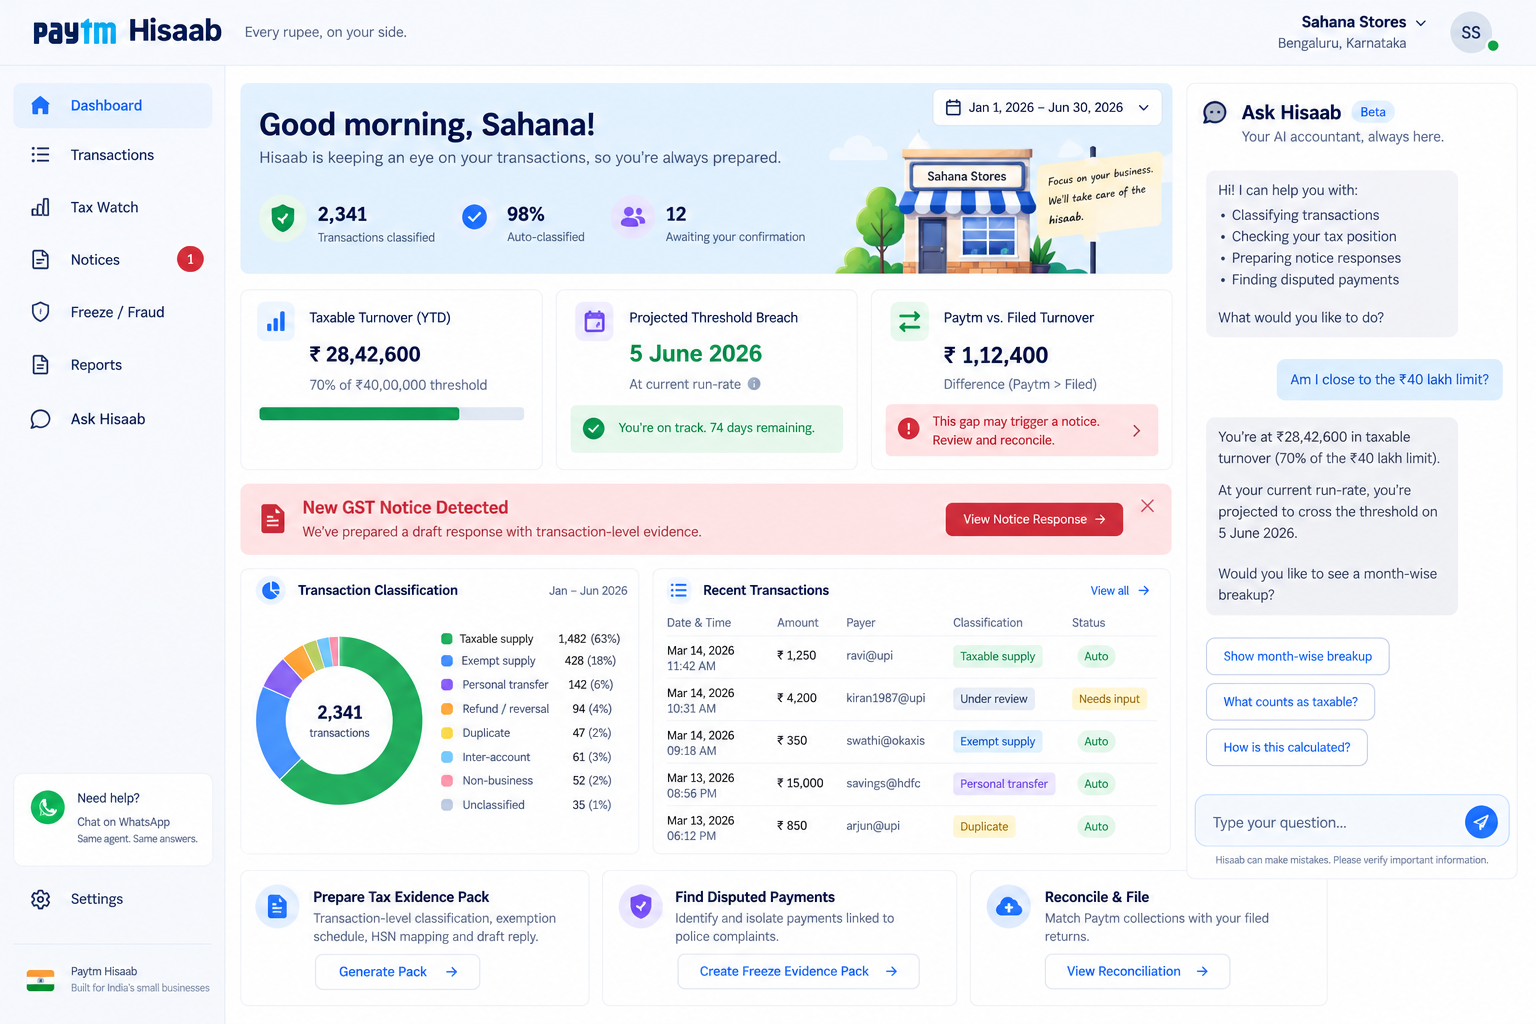
\includegraphics[width=\textwidth,height=0.70\textheight,keepaspectratio]{Paytm-Hisaab_website_look.png}
\end{center}
\vspace{0.1cm}
\hspace{0.05cm}{\scriptsize\color{muted}One surface: what every payment was classified as, how close she is to the threshold, and the packs. The same agent runs on WhatsApp, where she actually is.}
\note{{\color{navy}\bfseries\normalsize 8.~What the merchant sees}\par\vspace{0.55em}\textbf{0:20 --- a glance slide. Do not tour the UI.}
\\[0.4em]
One sentence: everything classified, how close she is to the threshold, and the
packs, on one surface.
\\[0.4em]
Then the WhatsApp point --- the same agent, where she actually is --- and advance.
\\[0.4em]
If someone asks whether this is built: the chat and the tools are live; this
screen is the product surface we are designing toward.}
\end{frame}

% ============================================================ 9. ARCHITECTURE
\begin{frame}{Built on Phinite}{Two agent graphs, four agents, ten deterministic skills}
\vspace{0.15cm}
\begin{columns}[T]
\begin{column}{0.53\textwidth}
{\scriptsize
\begin{tabular}{@{}L{1.75cm}L{4.7cm}@{}}
\multicolumn{2}{@{}l}{\color{navy}\bfseries\small hisaab-watch \;\scriptsize(autonomous: cron + API)}\\
\midrule
Provenance & proposes a tag and a reason for the hard credits \\
Evidence   & assembles packs: freeze evidence, then exemption schedules and HSN \\
\addlinespace[0.6em]
\multicolumn{2}{@{}l}{\color{navy}\bfseries\small hisaab-merchant \;\scriptsize(conversational: chat)}\\
\midrule
Merchant   & the conversation: attestation, alerts, Kannada \\
Escalation & decides when to stop and route to a human CA \\
\bottomrule
\end{tabular}}
\\[0.75em]
{\scriptsize\color{muted}The nightly pass writes its queue to the ledger; the chat reads it when she opens it. Deliberately \emph{not} a graph-to-graph call: a queue that outlives either run is what makes the handoff robust.}
\end{column}
\begin{column}{0.44\textwidth}
\card{5.7cm}{{\bfseries\color{navy}Permissions are the product}\\[0.4em]
\scriptsize Provenance proposes, \red{never commits}.\\[0.25em]
\scriptsize Merchant is the \emph{only} agent that can commit a tag.\\[0.25em]
\scriptsize Evidence is \red{read-only}. It cannot edit a classification to make a pack look better.\\[0.25em]
\scriptsize Escalation can \red{halt} any pack; a human approves.}
\\[0.5em]
\hspace{0.1cm}\begin{minipage}{5.7cm}{\scriptsize\color{muted}Ten tools run live against a hosted service. Every number in a pack traces back, in the trace, to the credit and the attestation behind it.}\end{minipage}
\end{column}
\end{columns}
\note{{\color{navy}\bfseries\normalsize 9.~Built on Phinite}\par\vspace{0.55em}\textbf{0:40 --- for the technical judges.}
\\[0.4em]
Two agent graphs, not four loose agents: \texttt{hisaab-watch} runs autonomously on
cron, \texttt{hisaab-merchant} is the conversation. The nightly pass writes a queue;
the chat reads it when she opens it --- deliberately not a graph-to-graph call,
because a queue that outlives either run is what makes the handoff robust.
\\[0.4em]
\textbf{Spend your time on the right-hand card.} The strongest line in it:
the Evidence agent is read-only --- \emph{the agent that builds the defence cannot
edit the evidence.} And only the Merchant agent can commit an attested tag.
\\[0.4em]
Those are enforced as Phinite tool policies, not conventions, and a denied call
shows up in the trace.}
\end{frame}

% ============================================================ 10. DESIGN DECISIONS
\begin{frame}{Four decisions that make it defensible}
\vspace{0.3cm}
\begin{columns}[T]
\begin{column}{0.48\textwidth}
\card{6.0cm}{{\bfseries\color{navy}1. Arithmetic lives in skills, not the model}\\[0.35em]
\scriptsize Turnover, projections and apportionment are deterministic Python: versioned, testable, traceable. Wrapping arithmetic in an LLM is the standard tell, and the trace would show it.}
\\[0.35em]
\card{6.0cm}{{\bfseries\color{navy}3. Refusing to guess is a feature}\\[0.35em]
\scriptsize An \texttt{unclassified} credit routed to the merchant costs one tap. A confident wrong tag inside an evidence pack is a catastrophe. We report the refusal rate honestly.}
\end{column}
\begin{column}{0.48\textwidth}
\card{6.0cm}{{\bfseries\color{navy}2. Attestation is the promotion boundary}\\[0.35em]
\scriptsize Nothing enters a production pack that the merchant has not confirmed. Sandbox to UAT to prod, with her tap as the gate.}
\\[0.35em]
\card{6.0cm}{{\bfseries\color{navy}4. Ground truth, so accuracy is a number}\\[0.35em]
\scriptsize We simulated a year of a shop's life from a known process, split into what Paytm can see and what really happened. Agents read only the visible half, which is why we quote error bars instead of vibes.}
\end{column}
\end{columns}
\note{{\color{navy}\bfseries\normalsize 10.~Four decisions}\par\vspace{0.55em}\textbf{0:35 --- the slide that separates you from a demo.}
\\[0.4em]
Lead with \#1: all arithmetic is deterministic Python, not model output. Wrapping
arithmetic in an LLM is the standard tell, and the trace would show it.
\\[0.4em]
Then \#3: refusing to guess is a feature. An \texttt{unclassified} credit costs one
tap; a confident wrong tag inside an evidence pack is a catastrophe.
\\[0.4em]
Skim \#2 and \#4 --- one clause each. \#4 is worth a beat if the room is technical:
we generated ground truth, so accuracy is a number instead of a claim.}
\end{frame}

% ============================================================ 11. DEMO / ATTESTATION
\begin{frame}{Demo $\cdot$ Sahana Stores, Jayanagar}{An ordinary Tuesday, before anything goes wrong}
\vspace{0.1cm}
\begin{columns}[T]
\begin{column}{0.48\textwidth}
{\scriptsize\color{muted}Tuesday 10 March. Thirty-nine credits came in over the weekend. The agent asks about \hi{three}.}
\\[0.4em]
\card{5.9cm}{{\kn\scriptsize ಭಾನುವಾರ ರಾತ್ರಿ ₹15,000. ನಿಮ್ಮ ಸ್ವಂತ ಹಣವೇ?}\\[0.25em]
{\color{muted}\scriptsize \qm{₹15,000 at 11:04pm Sunday, from your savings account. Your own money?}}\\[0.35em]
{\scriptsize\color{navy}\fbox{\kn ಹೌದು}\;\fbox{\kn ಇಲ್ಲ}}}
\\[0.4em]
{\scriptsize $\cdot$\; ₹7,500 from her husband, scanned at the shop QR\\[0.25em]
$\cdot$\; ₹4,850 from Raghu Shetty, who has bought twice before. A real sale, and the agent \emph{asks} rather than assumes.}
\\[0.4em]
{\scriptsize\color{muted}The other thirty-six settle silently, and a ₹23 payment nobody can place is left alone.}
\end{column}
\begin{column}{0.48\textwidth}
\ocard{amber}{6.1cm}{{\bfseries\color{amber}And yes, two of those three should not be there}\\[0.35em]
\scriptsize A business QR is not for personal money, and the terms say so. It arrives anyway: family, own top-ups, a chit payout. The rule does not prevent it. It only means \emph{nobody keeps a record of it.}}
\\[0.45em]
{\scriptsize Paytm already reads the signals: channel, linked VPAs, payer history. What no system has is the \hi{merchant's own answer}, given at the time, in her language, and kept.}
\\[0.45em]
{\scriptsize That record is what the next two slides are built from: first for the police, then for the department.}
\end{column}
\end{columns}
\note{{\color{navy}\bfseries\normalsize 11.~Demo --- an ordinary Tuesday (beat 1)}\par\vspace{0.55em}\textbf{0:45 --- or hand over to the live demo here.}
\\[0.4em]
Thirty-nine credits came in over the weekend, the agent asks about \textbf{three}.
Read the Kannada line if you can; otherwise read the gloss under it.
\\[0.4em]
\textbf{Do not hide from the right-hand card --- lead with it.} The mid-review
point was that personal money is not allowed on a business QR. Correct, and we say
so on the slide. The argument is that the rule does not stop it, it only means no
one records it, and an unrecorded credit is what an authority later reads as income.
\\[0.4em]
\textbf{Second half of that card matters just as much.} We are not claiming Paytm
does nothing. It already reads channel, linked VPAs and payer history. What no
system has is her own answer, captured while it is still knowable. That is the
product, and it is a smaller, truer claim than the one we started with.
\\[0.4em]
\textbf{Before going on stage:} confirm the attestation queue is whole ---
\texttt{pending\_total} must be 3. A rehearsal that taps through this beat spends the
queue, and Render needs a clear-cache redeploy to restore it.}
\end{frame}

% ============================================================ 12. DEMO / THE FREEZE
\begin{frame}{Demo $\cdot$ The emergency}{The account is frozen at 09:30 and the supplier payment is due}
\vspace{0.2cm}
\begin{columns}[T]
\begin{column}{0.46\textwidth}
{\scriptsize She sold someone 12kg of onions. That customer was three layers downstream of a fraud victim. She is not named in the FIR, which was filed in another state, and \hi{339 payments} came in that week.}
\\[0.5em]
\card{5.8cm}{{\bfseries\color{navy}The agent isolates it}\\[0.35em]
\scriptsize ₹4,200 on 21 March at 19:47, till POS01. Matched by UTR \emph{and independently} by amount and date.\\[0.3em]
\scriptsize The sale record comes with it: the POS bill, the items, the till and the minute.}
\end{column}
\begin{column}{0.49\textwidth}
\ocard{amber}{6.1cm}{{\bfseries\color{amber}And the decoy it did not choose}\\[0.35em]
\scriptsize A \emph{second} ₹4,200 that same week, from a regular customer. Listed in the pack, and explicitly \emph{not} named as the disputed one. Only the date separates them.}
\\[0.5em]
{\scriptsize Then it drafts the NCRP-CFCFRMS grievance, citing the judgments that only the \emph{disputed amount} should be lien-marked, not the whole account.}
\\[0.5em]
{\scriptsize\color{bad}\bfseries It never asserts that she is innocent.}\\[0.1em]
{\scriptsize\color{muted}Some frozen accounts genuinely are mule accounts. The agent assembles evidence; a human decides. Escalation holds the pack for approval.}
\end{column}
\end{columns}
\note{{\color{navy}\bfseries\normalsize 12.~Demo --- the emergency (beat 4)}\par\vspace{0.55em}\textbf{0:50 --- this is now the lead case. Give it the most time of the three.}
\\[0.4em]
Set the stakes in one sentence: account frozen at half nine, supplier payment due,
339 payments came in that week, and she is not named in the FIR.
\\[0.4em]
\textbf{Why this one leads.} She did nothing wrong and there is no rule she broke.
She sold onions to a customer who turned out to be laundering. Every objection
available against the tax case --- she should not have taken personal money on that
QR, she should have registered --- has no purchase here at all.
\\[0.4em]
The agent isolates ₹4,200 by UTR \emph{and independently} by amount and date, and
brings the POS bill with it --- the items, till POS01, 19:47.
\\[0.4em]
\textbf{The decoy is the point.} A second ₹4,200 that same week from a regular
customer, listed in the pack and explicitly not chosen. Anyone can match an amount;
the pack shows its work.
\\[0.4em]
Finish on the red line: it never asserts she is innocent. Some frozen accounts
genuinely are mule accounts. We assemble evidence; a human decides, and Escalation
holds the pack for approval.}
\end{frame}

% ============================================================ 13. DEMO / TAX
\begin{frame}{Demo $\cdot$ The warning, and the notice}{The same ledger, read for the other authority}
\vspace{0.15cm}
\begin{columns}[T]
\begin{column}{0.38\textwidth}
{\scriptsize\color{muted}Replayed as of 31 January:}
\\[0.35em]
\ocard{good}{4.8cm}{{\bfseries\color{ink}\scriptsize\qm{At your current rate you cross ₹40 lakh around {\color{bad}14 March}. You will need to register.}}\\[0.35em]
{\scriptsize\color{muted}\grn{43 days of warning}, and the date is computed, not typed.}}
\\[0.45em]
{\scriptsize\color{bad}\bfseries This beat is what makes the pitch safe.}\\[0.1em]
{\scriptsize\color{muted}Its first act on the tax side is telling her to register.}
\end{column}
\begin{column}{0.58\textwidth}
{\scriptsize\color{muted}Then the notice arrives, claiming {\color{bad}\bfseries ₹60.98L} of turnover:}
\\[0.3em]
{\scriptsize
\begin{tabular}{@{}lr@{\hskip 1.2em}l@{}}
\multicolumn{2}{@{}l}{\color{navy}\bfseries Aggregate turnover \quad ₹42.2L} & \sub{within \grn{1.6\%} of truth} \\
\midrule
Exempt supplies      & ₹31.3L & \sub{vegetables, loose rice} \\
Taxable supplies     & ₹10.9L & \sub{branded goods, oil, soap} \\
\addlinespace[0.45em]
\multicolumn{2}{@{}l}{\color{navy}\bfseries Not turnover at all \quad ₹18.8L} & \sub{every line traced} \\
\midrule
Her own accounts     & ₹7.4L & \sub{top-ups before supplier runs} \\
Family               & ₹6.1L & \sub{spouse, parent, in-law} \\
Loans, chit, gifts   & ₹4.3L & \sub{chit payout, festival gifts} \\
Refunds, duplicates  & ₹1.0L & \sub{crate returns, double-taps} \\
\bottomrule
\end{tabular}}
\\[0.45em]
{\scriptsize And it says plainly: \hi{the claim is wrong, and you \emph{did} cross ₹40 lakh on 14 March. You must register.}}
\end{column}
\end{columns}
\note{{\color{navy}\bfseries\normalsize 13.~Demo --- the warning and the notice (beats 2 and 3)}\par\vspace{0.55em}\textbf{0:50 --- two tax beats on one slide, deliberately compressed.}
\\[0.4em]
Left: replayed as of 31 January, the agent says she crosses ₹40 lakh around
14 March. \textbf{Say the red line out loud} --- its first act on the tax side is
telling her she owes a registration. That is what stops the room turning hostile.
\\[0.4em]
Right: the notice claims ₹60.98 lakh, and the pack answers it line by line, every
figure traceable to transaction IDs. Then the honest half:
\textbf{the claim is wrong, and she did cross ₹40 lakh, and she must register.}
\\[0.4em]
\textbf{If a judge diffs this against slide 5:} slide 5 shows seeded truth
(₹42.9L), this shows what our system computed (₹42.2L). The 1.6\% between them
\emph{is} the accuracy claim --- say that, do not hedge.
\\[0.4em]
\textbf{If pushed on the personal and own-account lines:} same answer as slide 11.
Those credits should not be on a business QR, they are there anyway, and the
alternative to classifying them is letting them be read as income.}
\end{frame}

% ============================================================ 14. NUMBERS
\begin{frame}{What we can actually prove}{One merchant, one year, 13,267 credits, scored against seeded truth}
\vspace{0.45cm}
\begin{columns}[T]
\begin{column}{0.33\textwidth}
\begin{center}\bignum{1.6\%}{error on aggregate turnover\\ (taxable share within 1\%)}\end{center}
\vspace{0.55cm}
\begin{center}\bignum{43 days}{of warning before the\\ threshold crossing}\end{center}
\end{column}
\begin{column}{0.33\textwidth}
\begin{center}\bignum{1.3 a day}{median questions asked.\\ 189 in a year, never over 3}\end{center}
\vspace{0.55cm}
\begin{center}\bignum{zero}{credits left untagged\\ across the whole year}\end{center}
\end{column}
\begin{column}{0.30\textwidth}
\card{3.8cm}{{\bfseries\color{navy}The honest baseline}\\[0.35em]
\scriptsize A 50-line rules-only classifier gets 99.3\% on sale vs not-a-sale, but catches only \red{77.8\%} of non-sale credits.\\[0.3em]
\scriptsize That residue alone puts two eval merchants on the \emph{wrong side} of ₹40L.\\[0.3em]
\scriptsize Closing it is what the agent plus one tap is for.}
\end{column}
\end{columns}
\vspace{0.45cm}
\hspace{0.1cm}{\scriptsize\color{muted}She corrected the agent 52 times that year. Those corrections are the ledger's strongest evidence, not its failures.}
\note{{\color{navy}\bfseries\normalsize 14.~What we can actually prove}\par\vspace{0.55em}\textbf{0:30 --- do not read all four. Pick two.}
\\[0.4em]
Lead with \textbf{1.6\%} error on turnover and \textbf{1.3 questions a day}. The
other two are there to be read, not narrated.
\\[0.4em]
\textbf{The credibility move is the box on the right} --- volunteer the weakness
before anyone finds it. A rules-only baseline gets 99.3\% on sale vs not-a-sale
but catches only 77.8\% of non-sale credits, and that residue alone puts two eval
merchants on the wrong side of ₹40 lakh. Closing it is what the agent plus one tap is for.
\\[0.4em]
Last line if you have the beat: she corrected the agent 52 times that year, and
those corrections are the ledger's strongest evidence, not its failures.}
\end{frame}

% ============================================================ 15. CLOSE
\begin{frame}{The line we do not cross}{Accuracy, not minimisation}
\vspace{0.3cm}
\begin{columns}[T]
\begin{column}{0.52\textwidth}
{\scriptsize
$\cdot$\; We \hi{never assert innocence} on a freeze. Some accounts really are mule accounts. We assemble evidence; a human decides.\\[0.5em]
$\cdot$\; We \hi{file nothing} with any authority. Artefacts only; the merchant or their CA files.\\[0.5em]
$\cdot$\; We compute what she \hi{genuinely owes} and say so plainly, including \qm{you crossed the threshold, you must register.}\\[0.5em]
$\cdot$\; We \hi{never assert a final liability}. We compute, show the workings, and route to a CA.\\[0.5em]
$\cdot$\; A business QR is \hi{not for personal money}. We do not excuse it. We record it, so it is not read as income.}
\end{column}
\begin{column}{0.44\textwidth}
\begin{tikzpicture}\node[rounded corners=4pt,fill=navy,text=white,inner sep=10pt,text width=5.7cm,align=left]{
{\bfseries Why this has to be Paytm}\\[0.45em]
\scriptsize The rail is the only place provenance is cheap. Everyone else arrives eighteen months late, when the answer is already unrecoverable.\\[0.45em]
\scriptsize A frozen merchant cannot transact at all: dead Soundbox and zero GMV the same morning, before it becomes the sign on the shutter, \emph{\qm{No UPI. Cash only.}}
};\end{tikzpicture}
\end{column}
\end{columns}
\vspace{0.4cm}
\begin{center}
{\large\color{navy}\bfseries Paytm Hisaab}\quad{\color{muted}every rupee, on your side.}
\end{center}
\note{{\color{navy}\bfseries\normalsize 15.~The line we do not cross}\par\vspace{0.55em}\textbf{0:30 --- the non-negotiables, fast, then land.}
\\[0.4em]
Run the five bullets at pace. The one to hit is the first: we never assert
innocence on a freeze. The last is the mid-review answer, on the slide on purpose.
\\[0.4em]
Then the navy box: provenance is cheap only on the rail, and a frozen merchant
stops transacting the same morning.
\\[0.4em]
Final line, unhurried: \emph{``Paytm Hisaab. Every rupee, on your side.''} Stop talking.
\\[0.5em]
{\scriptsize
{\color{navy}\bfseries --- Q\&A prep ---}
\\[0.3em]
\textbf{``Merchants may not take personal money on a business QR.''} Correct, and
slide 11 says so before you have to. It arrives anyway, and the alternative to
recording it is letting an authority read it as income. We are not defending the
behaviour --- we are refusing to let it become a liability.
\\[0.3em]
\textbf{``Paytm already tags transactions.''} It does, and we build on that rather
than around it: channel, linked VPAs and payer history feed the rules layer. What
no tag carries is her attestation --- the part an authority accepts, and the only
part she alone can give.
\\[0.3em]
\textbf{``No return mismatch?''} That check needs a \emph{registered} composition
dealer who filed a CMP-08 to disagree with. Ours is unregistered, which is why she
gets a notice at all; the eval split has one with four quarters seeded.
\\[0.3em]
\textbf{``Exempt vs taxable on a QR sale?''} Not per payment. We apportion by value
from that shop's own POS-billed ratio and label it an estimate. Labelling each sale
by its majority side understated taxable turnover threefold.
\\[0.3em]
\textbf{``Four LLM calls in a trenchcoat?''} Everything deterministic is a skill and
four agents is the ceiling. If twenty lines of Python replaces an agent, it should
have been a skill --- the trace shows which is which.
\\[0.3em]
\textbf{``No standing with the police.''} Agreed: Paytm supplies, the merchant
files. By design. Cash sales are real, out of scope, and on the slide.}}
\end{frame}

\end{document}
"
\ifdefined\shownotes
  \setbeamertemplate{note page}{%
    \usebeamercolor[fg]{normal text}%
    \vspace{0.2em}%
    {\scriptsize\color{muted}Paytm Hisaab \;$\cdot$\; speaker notes}\hfill
    {\scriptsize\color{muted}slide \insertframenumber\ of 15}\par
    \vspace{0.25em}{\color{ptmcyan}\rule{\textwidth}{1.5pt}}\par
    \vspace{0.55em}\footnotesize\raggedright\insertnote\par}
  \setbeameroption{show only notes}
\fi

\begin{document}

% ============================================================ 1. TITLE
{\setbeamertemplate{footline}{}
\begin{frame}[plain]
\vspace{0.9cm}
\begin{center}
{\fontsize{38}{42}\selectfont\bfseries\color{navy}Paytm\;\color{ink}Hisaab}\\[0.45em]
{\Large\color{muted}Every rupee, on your side.}\\[0.9em]
{\color{ptmcyan}\rule{2.8cm}{2.5pt}}\\[0.9em]
{\large\color{ink}The agent that lets a merchant account for their own money}\\[0.15em]
{\large\color{ink}when someone in authority demands an explanation.}\\[1.3em]
{\small\color{muted}Agent Labs Buildathon \;$\cdot$\; Phinite $\times$ Paytm \;$\cdot$\; Track 2: AI for Small Businesses}
\end{center}
\note{{\color{navy}\bfseries\normalsize 1.~Title}\par\vspace{0.55em}\textbf{0:10 --- open cold.} Do not read the title or the tagline off the slide.
\\[0.4em]
Say: \emph{``I want to tell you about a man in Haveri who opened an envelope.''} Then advance.
\\[0.4em]
Nothing on this slide needs explaining. The tagline lands at the end, not here.}
\end{frame}}

% ============================================================ 2. STORY
\begin{frame}{Haveri, 2025}{A vegetable vendor opens an envelope}
\vspace{0.05cm}
\begin{columns}[T]
\begin{column}{0.52\textwidth}
\vspace{0.15cm}
He sells vegetables. Vegetables are \hi{exempt} from GST.\\[0.6em]
He also took UPI, because Paytm asked him to.\\[0.6em]
Four years of credits into his account, added up and billed as income:
\begin{center}\vspace{0.1em}{\fontsize{30}{32}\selectfont\bfseries\color{bad}₹29 lakh}\end{center}
\end{column}
\begin{column}{0.44\textwidth}
\ocard{hairline}{5.4cm}{\centering
  {\color{muted}\scriptsize Within weeks, on shutters across Karnataka:}\\[0.6em]
  {\fontsize{20}{23}\selectfont\bfseries\color{ink}\qm{No UPI.\\ Cash only.}}\\[0.6em]
  {\color{muted}\scriptsize A statewide boycott, by the merchants who had just adopted it.}}
\end{column}
\end{columns}
\vspace{0.25cm}
\hspace{0.1cm}{\small\sub{Withdrawn for the traders who could \emph{show} what they sold. Most could not. And tax is no longer the only authority asking.}}
\note{{\color{navy}\bfseries\normalsize 2.~Haveri, 2025}\par\vspace{0.55em}\textbf{0:45 --- the hook. Tell it, do not summarise it.}
\\[0.4em]
Four beats, in this order: he sells vegetables; vegetables are exempt from GST;
he took UPI because \emph{we} asked him to; the department added up four years of
credits and sent him a bill for \textbf{₹29 lakh}.
\\[0.4em]
\textbf{Pause on the number.} Then the card: within weeks, shutters across Karnataka
read ``No UPI, cash only.'' Merchants we had just onboarded, boycotting the rail.
\\[0.4em]
Close on the bottom line --- the notices were withdrawn for traders who could
\emph{show} what they sold. Most could not. That verb is the whole product.
\\[0.4em]
\textbf{Then the bridge:} \emph{``and tax is no longer the only authority asking.''}
That sentence is doing the repositioning --- Haveri is not a tax story here, it is
the moment taking digital money became a liability. The sharper version of it is
two slides away.
\\[0.4em]
\textbf{Do not say this is happening right now.} It is 2025. The next slide is
what makes it current, and a judge who knows the episode will respect the distinction.}
\end{frame}

% ============================================================ 3. STILL HAPPENING
\begin{frame}{And this is not a 2025 story}{CAclubindia, last updated 02 September 2026: ten days ago}
\vspace{0.1cm}
\begin{center}

\includegraphics[width=12.4cm]{gst-notices-2026.png}
\end{center}
\vspace{0.35cm}
\card{13.1cm}{\scriptsize\qm{During August 2026, the GST Department issued a significant number of notices covering different financial years and involving a wide range of issues\ldots\ They covered matters such as ITC mismatches, ineligible credit, \hi{differences in turnover}, wrong GST classification or rate, \hi{exemption claims}, Reverse Charge Mechanism\ldots}}
\vspace{0.3cm}

\hspace{0.1cm}{\small Those two categories are the whole content of an evidence pack. And this is the \emph{slower} of the two authorities. The other one freezes the account first.}
\note{{\color{navy}\bfseries\normalsize 3.~And this is not a 2025 story}\par\vspace{0.55em}\textbf{0:25 --- fast. This slide exists to kill one objection.}
\\[0.4em]
Say: \emph{``That was last year. This was published ten days ago.''}
\\[0.4em]
Do not read the quote. Point at the two bolded phrases only ---
\textbf{differences in turnover} and \textbf{exemption claims} --- and say those
two categories are the entire content of what we build.
\\[0.4em]
\textbf{Land on the last line and move.} It is the handoff into the police
slide: this is the slower authority. The other one freezes first and asks
afterwards. Do not linger here --- tax is no longer the headline.}
\end{frame}

% ============================================================ 4. THE TRAP
\begin{frame}{Every rupee a merchant receives is now evidence}{Today it is only ever used against them}
\vspace{0.05cm}
\begin{columns}[T]
\begin{column}{0.47\textwidth}
\ocard{bad}{6.0cm}{{\bfseries\color{bad}The cyber-crime police}\\[0.35em]
\scriptsize Fraud money layers through accounts within minutes. The shop at the end of the chain, the one that sold someone a watermelon, is frozen. It did nothing wrong, is not named in the FIR, and finds out when a payment declines.}
\end{column}
\begin{column}{0.47\textwidth}
\card{6.1cm}{{\bfseries\color{navy}The tax department}\\[0.35em]
\scriptsize Compares UPI collections against filed returns and bills the difference. Registered traders too, with QR, wallet, card and cash deposits all in scope.}
\end{column}
\end{columns}
\vspace{0.4cm}
\begin{center}
{\large Both demand the same artefact: \hi{what was each rupee, actually?}}\\[0.3em]
{\small\color{muted}Paytm already sees more of this than anyone. What is missing is the \emph{merchant's own answer}, captured when it is still knowable.}
\end{center}
\vspace{0.15cm}
{\color{hairline}\hrule height 1pt}
\vspace{0.35em}
\hspace{0.05cm}{\scriptsize\bfseries\color{bad}What it costs Paytm:}~{\scriptsize a frozen merchant stops transacting that morning. A frightened one takes the QR down for good. Dead Soundbox, zero GMV, no lending origination.}
\note{{\color{navy}\bfseries\normalsize 4.~Every rupee is now evidence}\par\vspace{0.55em}\textbf{0:40 --- two authorities, one unanswerable question.}
\\[0.4em]
\textbf{Left card first and give it the time.} Fraud money layers within minutes,
and the shop at the end of the chain, \emph{the one that sold someone a watermelon},
gets frozen. It did nothing wrong, it is not named in the FIR, and it finds out
when a payment declines. Use the watermelon.
\\[0.4em]
Right card briskly: the department reconciles collections against filed returns
and bills the difference. One sentence, then move.
\\[0.4em]
Then the pivot: both demand the same artefact --- what was each rupee, actually.
\\[0.4em]
\textbf{Say the grey line as written.} We do \emph{not} claim Paytm does nothing
with this data --- it tags plenty. The gap is the merchant's own answer, captured
when it is still knowable. Claiming otherwise in this room gets corrected.
\\[0.4em]
\textbf{Slow down for the red line.} This is the business case, not a footnote:
a frozen merchant stops transacting that morning, a frightened one takes the QR
down for good. Dead Soundbox, zero GMV, no lending origination.}
\end{frame}

% ============================================================ 5. THE BAR
\begin{frame}{Gross credits are not turnover}{One shop, one year, ₹60.98 lakh of credits}
\vspace{0.1cm}
\begin{center}
\begin{tikzpicture}[x=1cm,y=1cm]
% --- what the notice counts
\node[anchor=west,font=\scriptsize\bfseries,text=bad] at (-0.05,1.80) {WHAT THE NOTICE COUNTS AS TURNOVER};
\fill[bad!85,rounded corners=2pt] (0,1.06) rectangle (11.4,1.60);
\node[font=\small\bfseries,text=white] at (5.7,1.33) {₹60.98 lakh};

% --- what actually happened   (1 lakh = 0.18696 cm, so the bars are the same length)
\node[anchor=west,font=\scriptsize\bfseries,text=navy] at (-0.05,0.66) {WHAT ACTUALLY HAPPENED};
\fill[good!80,rounded corners=2pt]  (0,-0.08)     rectangle (6.001,0.46);
\fill[good!45]                      (6.001,-0.08) rectangle (8.002,0.46);
\fill[ptmcyan!70]                   (8.002,-0.08) rectangle (9.385,0.46);
\fill[navy!55]                      (9.385,-0.08) rectangle (10.451,0.46);
\fill[amber!70]                     (10.451,-0.08)rectangle (11.255,0.46);
\fill[muted!60,rounded corners=2pt] (11.255,-0.08)rectangle (11.4,0.46);

% brackets
\draw[navy,line width=0.8pt] (0,-0.22) -- (0,-0.36) -- (8.002,-0.36) -- (8.002,-0.22);
\node[anchor=north,font=\scriptsize,text=navy,align=center] at (4.0,-0.38)
  {\bfseries ₹42.9L aggregate turnover\quad{\color{muted}\scriptsize exempt ₹32.1L + taxable ₹10.7L}};
\draw[bad,line width=0.8pt] (8.002,-0.22) -- (8.002,-0.36) -- (11.4,-0.36) -- (11.4,-0.22);
\node[anchor=north,font=\scriptsize,text=bad,align=center] at (9.7,-0.38)
  {\bfseries ₹18.1L that is not turnover at all};

% legend
\node[font=\scriptsize,text=ink] at (5.7,-1.02) {%
\textcolor{good!80}{$\blacksquare$}~Exempt sales \quad
\textcolor{good!45}{$\blacksquare$}~Taxable sales \quad
\textcolor{ptmcyan!70}{$\blacksquare$}~Her own accounts ₹7.4L};
\node[font=\scriptsize,text=ink] at (5.7,-1.40) {%
\textcolor{navy!55}{$\blacksquare$}~Family ₹5.7L \quad
\textcolor{amber!70}{$\blacksquare$}~Loans, chit, gifts ₹4.3L \quad
\textcolor{muted!60}{$\blacksquare$}~Refunds \& duplicates ₹0.7L};
\end{tikzpicture}
\end{center}
\vspace{0.15cm}
\hspace{0.1cm}{\small\sub{Personal money does not belong on a business QR. It arrives anyway, reads as turnover, and hides the one credit the police will ask about.}}
\note{{\color{navy}\bfseries\normalsize 5.~Gross credits are not turnover}\par\vspace{0.55em}\textbf{0:45 --- the hinge of the pitch. Let the picture work.}
\\[0.4em]
Say: \emph{``One shop, one year, ₹60.98 lakh of credits. The red bar is what the
notice counts as turnover --- all of it.''}
\\[0.4em]
Then the bottom bar. \textbf{Stop talking for two seconds} and let them read it.
\\[0.4em]
₹42.9L really is turnover, and we say so. ₹18.1L is not: her savings account, her
husband, a chit payout, a double-tap on the Soundbox.
\\[0.4em]
\textbf{Get in front of the obvious objection.} Personal money is not supposed to
touch a business QR. Say so first, then say it arrives anyway --- that is an
observation about merchants, not a loophole we are selling. The rule does not stop
it; it only means no one is keeping a record of it.
\\[0.4em]
\textbf{And close on the second use.} This volume is also why she cannot find the
one credit the police care about. Same bar, same problem, and the freeze slide
pays it off.
\\[0.4em]
If challenged on the numbers: seeded ground truth from our generator, not an
estimate. Accuracy against it is slide 14.}
\end{frame}

% ============================================================ 6. INSIGHT
\begin{frame}{The insight}{Most teams would build the tax tool \emph{or} the fraud tool. They are the same engine.}
\vspace{0.15cm}
\begin{center}
\begin{tikzpicture}[font=\scriptsize]
\node[rounded corners=4pt,fill=navy,text=white,inner sep=7pt,align=center,text width=3.5cm]
  (eng) {\bfseries\small Provenance Ledger\\[0.15em] a merchant-attested label on every incoming credit};
\node[rounded corners=4pt,fill=tint,draw=bad,inner sep=6pt,align=center,text width=4.0cm]
  (tax) at ($(eng.east)+(3.7,0.78)$) {\bfseries The disputed rupee\\ freeze pack, NCRP grievance};
\node[rounded corners=4pt,fill=tint,draw=hairline,inner sep=6pt,align=center,text width=4.0cm]
  (fra) at ($(eng.east)+(3.7,-0.78)$) {\bfseries Defensible turnover\\ threshold watch, notice pack};
\draw[-{Stealth[length=2.5mm]},ptmcyan,line width=1.3pt] (eng.east) -- ++(0.5,0) |- (tax.west);
\draw[-{Stealth[length=2.5mm]},ptmcyan,line width=1.3pt] (eng.east) -- ++(0.5,0) |- (fra.west);
\node[anchor=east,text width=2.9cm,align=right,text=muted] at ($(eng.west)+(-0.35,0)$)
  {Both are downstream \emph{reads} of one ledger. Two output formats, not two products.};
\end{tikzpicture}
\end{center}
\vspace{0.1cm}
\begin{center}
\begin{tikzpicture}\node[rounded corners=4pt,fill=tint,inner sep=8pt,text width=11.2cm,align=center]{
{\bfseries\color{navy}The wedge nobody else has.}\\[0.25em]
\small Khatabook and Vyapar keep books after the fact. ClearTax files after the fact.\\
Neither sits on the rail \emph{at the moment money moves}. Paytm does.\\[0.25em]
\small Classification is cheap at the instant of the transaction,\\ and unrecoverable eighteen months later.
};\end{tikzpicture}
\end{center}
\note{{\color{navy}\bfseries\normalsize 6.~The insight}\par\vspace{0.55em}\textbf{0:40 --- why this is one product, not two.}
\\[0.4em]
Say: \emph{``Most teams would build the fraud tool or the tax tool. They are the
same engine.''} Both are downstream reads of one ledger --- two output formats,
and the freeze pack is the one we lead with.
\\[0.4em]
Then the wedge, and say it slowly because it is the defensible-moat answer:
Khatabook and Vyapar keep books after the fact, ClearTax files after the fact.
Neither sits on the rail at the moment money moves. \textbf{Paytm does.}
\\[0.4em]
Landing line: classification is cheap and accurate at the instant of the
transaction, and unrecoverable eighteen months later when the notice arrives.}
\end{frame}

% ============================================================ 7. THE ENGINE
\begin{frame}{The engine}{Eight tags, one tap}
\vspace{0.15cm}
\begin{columns}[T]
\begin{column}{0.45\textwidth}
{\color{navy}\bfseries\small Every incoming credit gets one tag}\\[0.4em]
{\scriptsize
\begin{tabular}{@{}ll@{}}
\texttt{taxable\_supply}    & ordinary sale \\
\texttt{exempt\_supply}     & vegetables, milk, loose rice \\
\texttt{personal\_transfer} & spouse, parent, sibling \\
\texttt{inter\_account}     & her own money \\
\texttt{refund\_reversal}   & money back from a vendor \\
\texttt{duplicate}          & paid twice, one refunded \\
\texttt{non\_business}      & loan, chit payout, gift \\
{\color{bad}\texttt{unclassified}} & {\color{bad}not enough signal: ask her} \\
\end{tabular}}
\\[0.75em]
{\scriptsize\color{muted}98.6\% are ordinary sales, settled by rules. The agent reasons only about the 1.4\% that need judgement.}
\end{column}
\begin{column}{0.51\textwidth}
\card{6.6cm}{{\bfseries\color{navy}The agent proposes. The merchant attests.}\\[0.4em]
\scriptsize You cannot infer \qm{my husband sent this} from a QR payment. The agent proposes a tag \emph{with its reason}; she confirms with one tap, in Kannada, batched daily.\\[0.45em]
\scriptsize Not a fallback. A ledger she attested \emph{at the time} survives a hearing. An algorithm's guess, made under duress a year later, does not.}
\\[0.55em]
\hspace{0.15cm}\begin{minipage}{6.6cm}
{\bfseries\color{navy}\small Budget: at most 3 questions a day.}\\[0.15em]
{\scriptsize\color{muted}Over a simulated year: \hi{189 questions, median 1.3 a day}. Ask more and the product is dead.}
\end{minipage}
\end{column}
\end{columns}
\note{{\color{navy}\bfseries\normalsize 7.~The engine}\par\vspace{0.55em}\textbf{0:45 --- the mechanism. Do not read the tag list.}
\\[0.4em]
Gesture at the eight tags, say ``eight labels, every incoming credit gets one,''
and move to the right-hand card, which is the real content.
\\[0.4em]
\textbf{The line that matters:} you cannot infer ``my husband sent this'' from a
QR payment. So the agent proposes a tag \emph{with its reason} and she confirms
with one tap. This is not a fallback --- a ledger she attested contemporaneously
survives a hearing; an algorithm's guess produced under duress a year later does not.
\\[0.4em]
Then the budget: at most three questions a day, and we measured 189 across a
year, median 1.3. Ask more than that and the product is dead.
\\[0.4em]
If asked about cost: 98.6\% are ordinary sales settled by rules. The model only
sees the 1.4\% that need judgement.}
\end{frame}

% ============================================================ 8. PRODUCT
\begin{frame}{What the merchant sees}
\vspace{-0.1cm}
\begin{center}
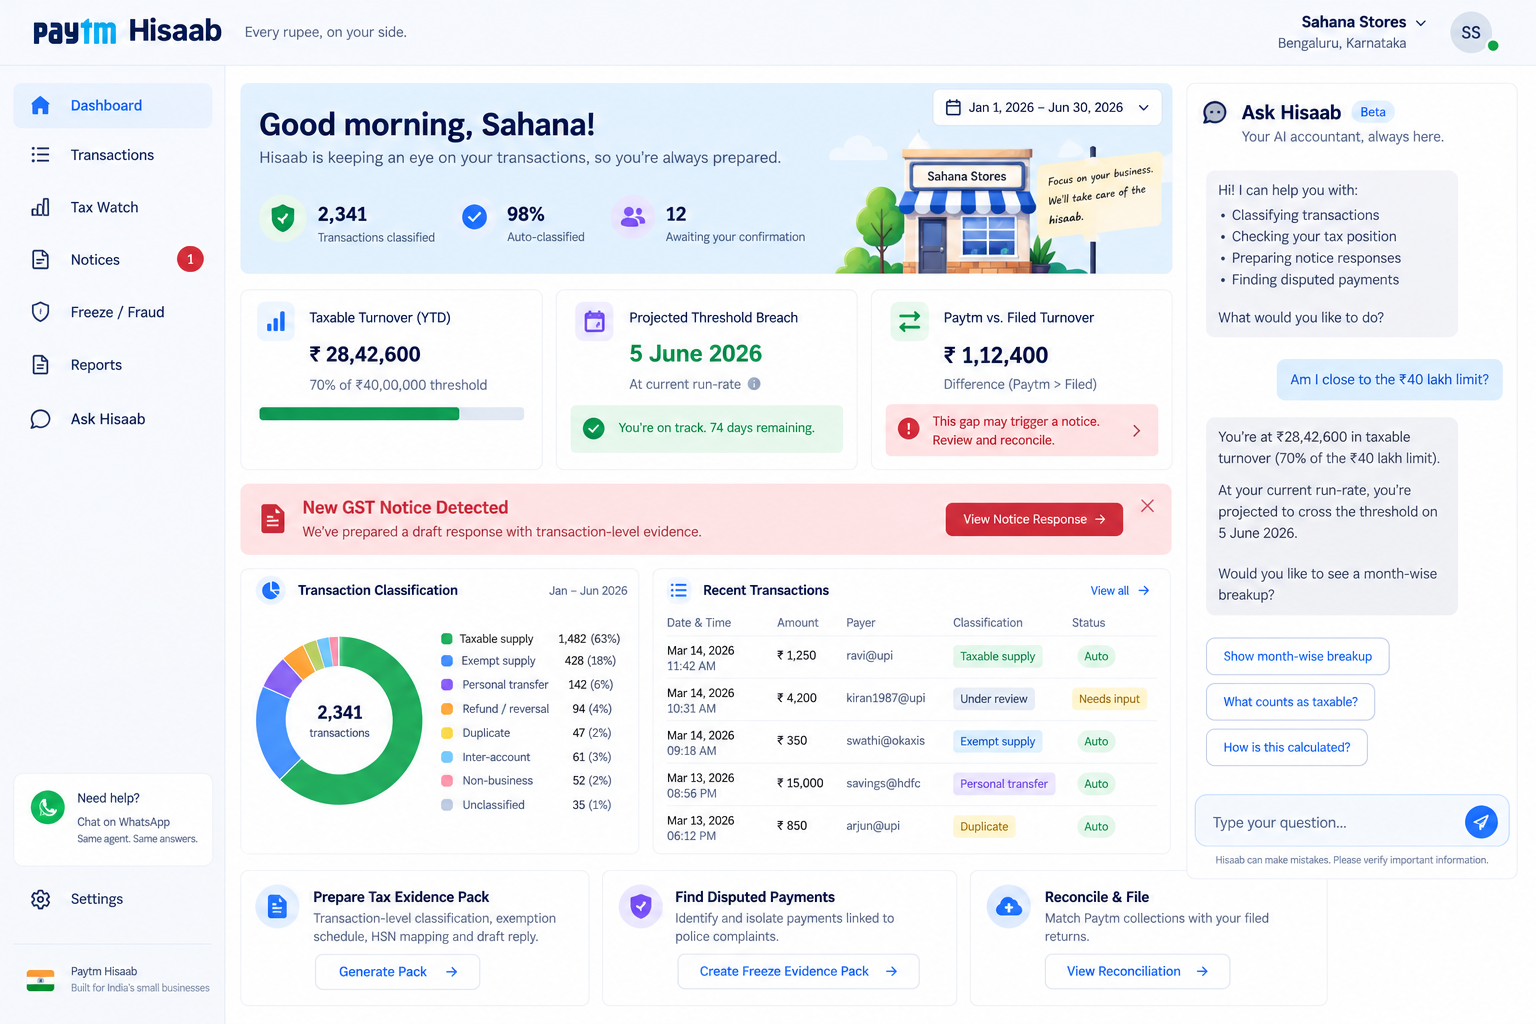
\includegraphics[width=\textwidth,height=0.70\textheight,keepaspectratio]{Paytm-Hisaab_website_look.png}
\end{center}
\vspace{0.1cm}
\hspace{0.05cm}{\scriptsize\color{muted}One surface: what every payment was classified as, how close she is to the threshold, and the packs. The same agent runs on WhatsApp, where she actually is.}
\note{{\color{navy}\bfseries\normalsize 8.~What the merchant sees}\par\vspace{0.55em}\textbf{0:20 --- a glance slide. Do not tour the UI.}
\\[0.4em]
One sentence: everything classified, how close she is to the threshold, and the
packs, on one surface.
\\[0.4em]
Then the WhatsApp point --- the same agent, where she actually is --- and advance.
\\[0.4em]
If someone asks whether this is built: the chat and the tools are live; this
screen is the product surface we are designing toward.}
\end{frame}

% ============================================================ 9. ARCHITECTURE
\begin{frame}{Built on Phinite}{Two agent graphs, four agents, ten deterministic skills}
\vspace{0.15cm}
\begin{columns}[T]
\begin{column}{0.53\textwidth}
{\scriptsize
\begin{tabular}{@{}L{1.75cm}L{4.7cm}@{}}
\multicolumn{2}{@{}l}{\color{navy}\bfseries\small hisaab-watch \;\scriptsize(autonomous: cron + API)}\\
\midrule
Provenance & proposes a tag and a reason for the hard credits \\
Evidence   & assembles packs: freeze evidence, then exemption schedules and HSN \\
\addlinespace[0.6em]
\multicolumn{2}{@{}l}{\color{navy}\bfseries\small hisaab-merchant \;\scriptsize(conversational: chat)}\\
\midrule
Merchant   & the conversation: attestation, alerts, Kannada \\
Escalation & decides when to stop and route to a human CA \\
\bottomrule
\end{tabular}}
\\[0.75em]
{\scriptsize\color{muted}The nightly pass writes its queue to the ledger; the chat reads it when she opens it. Deliberately \emph{not} a graph-to-graph call: a queue that outlives either run is what makes the handoff robust.}
\end{column}
\begin{column}{0.44\textwidth}
\card{5.7cm}{{\bfseries\color{navy}Permissions are the product}\\[0.4em]
\scriptsize Provenance proposes, \red{never commits}.\\[0.25em]
\scriptsize Merchant is the \emph{only} agent that can commit a tag.\\[0.25em]
\scriptsize Evidence is \red{read-only}. It cannot edit a classification to make a pack look better.\\[0.25em]
\scriptsize Escalation can \red{halt} any pack; a human approves.}
\\[0.5em]
\hspace{0.1cm}\begin{minipage}{5.7cm}{\scriptsize\color{muted}Ten tools run live against a hosted service. Every number in a pack traces back, in the trace, to the credit and the attestation behind it.}\end{minipage}
\end{column}
\end{columns}
\note{{\color{navy}\bfseries\normalsize 9.~Built on Phinite}\par\vspace{0.55em}\textbf{0:40 --- for the technical judges.}
\\[0.4em]
Two agent graphs, not four loose agents: \texttt{hisaab-watch} runs autonomously on
cron, \texttt{hisaab-merchant} is the conversation. The nightly pass writes a queue;
the chat reads it when she opens it --- deliberately not a graph-to-graph call,
because a queue that outlives either run is what makes the handoff robust.
\\[0.4em]
\textbf{Spend your time on the right-hand card.} The strongest line in it:
the Evidence agent is read-only --- \emph{the agent that builds the defence cannot
edit the evidence.} And only the Merchant agent can commit an attested tag.
\\[0.4em]
Those are enforced as Phinite tool policies, not conventions, and a denied call
shows up in the trace.}
\end{frame}

% ============================================================ 10. DESIGN DECISIONS
\begin{frame}{Four decisions that make it defensible}
\vspace{0.3cm}
\begin{columns}[T]
\begin{column}{0.48\textwidth}
\card{6.0cm}{{\bfseries\color{navy}1. Arithmetic lives in skills, not the model}\\[0.35em]
\scriptsize Turnover, projections and apportionment are deterministic Python: versioned, testable, traceable. Wrapping arithmetic in an LLM is the standard tell, and the trace would show it.}
\\[0.35em]
\card{6.0cm}{{\bfseries\color{navy}3. Refusing to guess is a feature}\\[0.35em]
\scriptsize An \texttt{unclassified} credit routed to the merchant costs one tap. A confident wrong tag inside an evidence pack is a catastrophe. We report the refusal rate honestly.}
\end{column}
\begin{column}{0.48\textwidth}
\card{6.0cm}{{\bfseries\color{navy}2. Attestation is the promotion boundary}\\[0.35em]
\scriptsize Nothing enters a production pack that the merchant has not confirmed. Sandbox to UAT to prod, with her tap as the gate.}
\\[0.35em]
\card{6.0cm}{{\bfseries\color{navy}4. Ground truth, so accuracy is a number}\\[0.35em]
\scriptsize We simulated a year of a shop's life from a known process, split into what Paytm can see and what really happened. Agents read only the visible half, which is why we quote error bars instead of vibes.}
\end{column}
\end{columns}
\note{{\color{navy}\bfseries\normalsize 10.~Four decisions}\par\vspace{0.55em}\textbf{0:35 --- the slide that separates you from a demo.}
\\[0.4em]
Lead with \#1: all arithmetic is deterministic Python, not model output. Wrapping
arithmetic in an LLM is the standard tell, and the trace would show it.
\\[0.4em]
Then \#3: refusing to guess is a feature. An \texttt{unclassified} credit costs one
tap; a confident wrong tag inside an evidence pack is a catastrophe.
\\[0.4em]
Skim \#2 and \#4 --- one clause each. \#4 is worth a beat if the room is technical:
we generated ground truth, so accuracy is a number instead of a claim.}
\end{frame}

% ============================================================ 11. DEMO / ATTESTATION
\begin{frame}{Demo $\cdot$ Sahana Stores, Jayanagar}{An ordinary Tuesday, before anything goes wrong}
\vspace{0.1cm}
\begin{columns}[T]
\begin{column}{0.48\textwidth}
{\scriptsize\color{muted}Tuesday 10 March. Thirty-nine credits came in over the weekend. The agent asks about \hi{three}.}
\\[0.4em]
\card{5.9cm}{{\kn\scriptsize ಭಾನುವಾರ ರಾತ್ರಿ ₹15,000. ನಿಮ್ಮ ಸ್ವಂತ ಹಣವೇ?}\\[0.25em]
{\color{muted}\scriptsize \qm{₹15,000 at 11:04pm Sunday, from your savings account. Your own money?}}\\[0.35em]
{\scriptsize\color{navy}\fbox{\kn ಹೌದು}\;\fbox{\kn ಇಲ್ಲ}}}
\\[0.4em]
{\scriptsize $\cdot$\; ₹7,500 from her husband, scanned at the shop QR\\[0.25em]
$\cdot$\; ₹4,850 from Raghu Shetty, who has bought twice before. A real sale, and the agent \emph{asks} rather than assumes.}
\\[0.4em]
{\scriptsize\color{muted}The other thirty-six settle silently, and a ₹23 payment nobody can place is left alone.}
\end{column}
\begin{column}{0.48\textwidth}
\ocard{amber}{6.1cm}{{\bfseries\color{amber}And yes, two of those three should not be there}\\[0.35em]
\scriptsize A business QR is not for personal money, and the terms say so. It arrives anyway: family, own top-ups, a chit payout. The rule does not prevent it. It only means \emph{nobody keeps a record of it.}}
\\[0.45em]
{\scriptsize Paytm already reads the signals: channel, linked VPAs, payer history. What no system has is the \hi{merchant's own answer}, given at the time, in her language, and kept.}
\\[0.45em]
{\scriptsize That record is what the next two slides are built from: first for the police, then for the department.}
\end{column}
\end{columns}
\note{{\color{navy}\bfseries\normalsize 11.~Demo --- an ordinary Tuesday (beat 1)}\par\vspace{0.55em}\textbf{0:45 --- or hand over to the live demo here.}
\\[0.4em]
Thirty-nine credits came in over the weekend, the agent asks about \textbf{three}.
Read the Kannada line if you can; otherwise read the gloss under it.
\\[0.4em]
\textbf{Do not hide from the right-hand card --- lead with it.} The mid-review
point was that personal money is not allowed on a business QR. Correct, and we say
so on the slide. The argument is that the rule does not stop it, it only means no
one records it, and an unrecorded credit is what an authority later reads as income.
\\[0.4em]
\textbf{Second half of that card matters just as much.} We are not claiming Paytm
does nothing. It already reads channel, linked VPAs and payer history. What no
system has is her own answer, captured while it is still knowable. That is the
product, and it is a smaller, truer claim than the one we started with.
\\[0.4em]
\textbf{Before going on stage:} confirm the attestation queue is whole ---
\texttt{pending\_total} must be 3. A rehearsal that taps through this beat spends the
queue, and Render needs a clear-cache redeploy to restore it.}
\end{frame}

% ============================================================ 12. DEMO / THE FREEZE
\begin{frame}{Demo $\cdot$ The emergency}{The account is frozen at 09:30 and the supplier payment is due}
\vspace{0.2cm}
\begin{columns}[T]
\begin{column}{0.46\textwidth}
{\scriptsize She sold someone 12kg of onions. That customer was three layers downstream of a fraud victim. She is not named in the FIR, which was filed in another state, and \hi{339 payments} came in that week.}
\\[0.5em]
\card{5.8cm}{{\bfseries\color{navy}The agent isolates it}\\[0.35em]
\scriptsize ₹4,200 on 21 March at 19:47, till POS01. Matched by UTR \emph{and independently} by amount and date.\\[0.3em]
\scriptsize The sale record comes with it: the POS bill, the items, the till and the minute.}
\end{column}
\begin{column}{0.49\textwidth}
\ocard{amber}{6.1cm}{{\bfseries\color{amber}And the decoy it did not choose}\\[0.35em]
\scriptsize A \emph{second} ₹4,200 that same week, from a regular customer. Listed in the pack, and explicitly \emph{not} named as the disputed one. Only the date separates them.}
\\[0.5em]
{\scriptsize Then it drafts the NCRP-CFCFRMS grievance, citing the judgments that only the \emph{disputed amount} should be lien-marked, not the whole account.}
\\[0.5em]
{\scriptsize\color{bad}\bfseries It never asserts that she is innocent.}\\[0.1em]
{\scriptsize\color{muted}Some frozen accounts genuinely are mule accounts. The agent assembles evidence; a human decides. Escalation holds the pack for approval.}
\end{column}
\end{columns}
\note{{\color{navy}\bfseries\normalsize 12.~Demo --- the emergency (beat 4)}\par\vspace{0.55em}\textbf{0:50 --- this is now the lead case. Give it the most time of the three.}
\\[0.4em]
Set the stakes in one sentence: account frozen at half nine, supplier payment due,
339 payments came in that week, and she is not named in the FIR.
\\[0.4em]
\textbf{Why this one leads.} She did nothing wrong and there is no rule she broke.
She sold onions to a customer who turned out to be laundering. Every objection
available against the tax case --- she should not have taken personal money on that
QR, she should have registered --- has no purchase here at all.
\\[0.4em]
The agent isolates ₹4,200 by UTR \emph{and independently} by amount and date, and
brings the POS bill with it --- the items, till POS01, 19:47.
\\[0.4em]
\textbf{The decoy is the point.} A second ₹4,200 that same week from a regular
customer, listed in the pack and explicitly not chosen. Anyone can match an amount;
the pack shows its work.
\\[0.4em]
Finish on the red line: it never asserts she is innocent. Some frozen accounts
genuinely are mule accounts. We assemble evidence; a human decides, and Escalation
holds the pack for approval.}
\end{frame}

% ============================================================ 13. DEMO / TAX
\begin{frame}{Demo $\cdot$ The warning, and the notice}{The same ledger, read for the other authority}
\vspace{0.15cm}
\begin{columns}[T]
\begin{column}{0.38\textwidth}
{\scriptsize\color{muted}Replayed as of 31 January:}
\\[0.35em]
\ocard{good}{4.8cm}{{\bfseries\color{ink}\scriptsize\qm{At your current rate you cross ₹40 lakh around {\color{bad}14 March}. You will need to register.}}\\[0.35em]
{\scriptsize\color{muted}\grn{43 days of warning}, and the date is computed, not typed.}}
\\[0.45em]
{\scriptsize\color{bad}\bfseries This beat is what makes the pitch safe.}\\[0.1em]
{\scriptsize\color{muted}Its first act on the tax side is telling her to register.}
\end{column}
\begin{column}{0.58\textwidth}
{\scriptsize\color{muted}Then the notice arrives, claiming {\color{bad}\bfseries ₹60.98L} of turnover:}
\\[0.3em]
{\scriptsize
\begin{tabular}{@{}lr@{\hskip 1.2em}l@{}}
\multicolumn{2}{@{}l}{\color{navy}\bfseries Aggregate turnover \quad ₹42.2L} & \sub{within \grn{1.6\%} of truth} \\
\midrule
Exempt supplies      & ₹31.3L & \sub{vegetables, loose rice} \\
Taxable supplies     & ₹10.9L & \sub{branded goods, oil, soap} \\
\addlinespace[0.45em]
\multicolumn{2}{@{}l}{\color{navy}\bfseries Not turnover at all \quad ₹18.8L} & \sub{every line traced} \\
\midrule
Her own accounts     & ₹7.4L & \sub{top-ups before supplier runs} \\
Family               & ₹6.1L & \sub{spouse, parent, in-law} \\
Loans, chit, gifts   & ₹4.3L & \sub{chit payout, festival gifts} \\
Refunds, duplicates  & ₹1.0L & \sub{crate returns, double-taps} \\
\bottomrule
\end{tabular}}
\\[0.45em]
{\scriptsize And it says plainly: \hi{the claim is wrong, and you \emph{did} cross ₹40 lakh on 14 March. You must register.}}
\end{column}
\end{columns}
\note{{\color{navy}\bfseries\normalsize 13.~Demo --- the warning and the notice (beats 2 and 3)}\par\vspace{0.55em}\textbf{0:50 --- two tax beats on one slide, deliberately compressed.}
\\[0.4em]
Left: replayed as of 31 January, the agent says she crosses ₹40 lakh around
14 March. \textbf{Say the red line out loud} --- its first act on the tax side is
telling her she owes a registration. That is what stops the room turning hostile.
\\[0.4em]
Right: the notice claims ₹60.98 lakh, and the pack answers it line by line, every
figure traceable to transaction IDs. Then the honest half:
\textbf{the claim is wrong, and she did cross ₹40 lakh, and she must register.}
\\[0.4em]
\textbf{If a judge diffs this against slide 5:} slide 5 shows seeded truth
(₹42.9L), this shows what our system computed (₹42.2L). The 1.6\% between them
\emph{is} the accuracy claim --- say that, do not hedge.
\\[0.4em]
\textbf{If pushed on the personal and own-account lines:} same answer as slide 11.
Those credits should not be on a business QR, they are there anyway, and the
alternative to classifying them is letting them be read as income.}
\end{frame}

% ============================================================ 14. NUMBERS
\begin{frame}{What we can actually prove}{One merchant, one year, 13,267 credits, scored against seeded truth}
\vspace{0.45cm}
\begin{columns}[T]
\begin{column}{0.33\textwidth}
\begin{center}\bignum{1.6\%}{error on aggregate turnover\\ (taxable share within 1\%)}\end{center}
\vspace{0.55cm}
\begin{center}\bignum{43 days}{of warning before the\\ threshold crossing}\end{center}
\end{column}
\begin{column}{0.33\textwidth}
\begin{center}\bignum{1.3 a day}{median questions asked.\\ 189 in a year, never over 3}\end{center}
\vspace{0.55cm}
\begin{center}\bignum{zero}{credits left untagged\\ across the whole year}\end{center}
\end{column}
\begin{column}{0.30\textwidth}
\card{3.8cm}{{\bfseries\color{navy}The honest baseline}\\[0.35em]
\scriptsize A 50-line rules-only classifier gets 99.3\% on sale vs not-a-sale, but catches only \red{77.8\%} of non-sale credits.\\[0.3em]
\scriptsize That residue alone puts two eval merchants on the \emph{wrong side} of ₹40L.\\[0.3em]
\scriptsize Closing it is what the agent plus one tap is for.}
\end{column}
\end{columns}
\vspace{0.45cm}
\hspace{0.1cm}{\scriptsize\color{muted}She corrected the agent 52 times that year. Those corrections are the ledger's strongest evidence, not its failures.}
\note{{\color{navy}\bfseries\normalsize 14.~What we can actually prove}\par\vspace{0.55em}\textbf{0:30 --- do not read all four. Pick two.}
\\[0.4em]
Lead with \textbf{1.6\%} error on turnover and \textbf{1.3 questions a day}. The
other two are there to be read, not narrated.
\\[0.4em]
\textbf{The credibility move is the box on the right} --- volunteer the weakness
before anyone finds it. A rules-only baseline gets 99.3\% on sale vs not-a-sale
but catches only 77.8\% of non-sale credits, and that residue alone puts two eval
merchants on the wrong side of ₹40 lakh. Closing it is what the agent plus one tap is for.
\\[0.4em]
Last line if you have the beat: she corrected the agent 52 times that year, and
those corrections are the ledger's strongest evidence, not its failures.}
\end{frame}

% ============================================================ 15. CLOSE
\begin{frame}{The line we do not cross}{Accuracy, not minimisation}
\vspace{0.3cm}
\begin{columns}[T]
\begin{column}{0.52\textwidth}
{\scriptsize
$\cdot$\; We \hi{never assert innocence} on a freeze. Some accounts really are mule accounts. We assemble evidence; a human decides.\\[0.5em]
$\cdot$\; We \hi{file nothing} with any authority. Artefacts only; the merchant or their CA files.\\[0.5em]
$\cdot$\; We compute what she \hi{genuinely owes} and say so plainly, including \qm{you crossed the threshold, you must register.}\\[0.5em]
$\cdot$\; We \hi{never assert a final liability}. We compute, show the workings, and route to a CA.\\[0.5em]
$\cdot$\; A business QR is \hi{not for personal money}. We do not excuse it. We record it, so it is not read as income.}
\end{column}
\begin{column}{0.44\textwidth}
\begin{tikzpicture}\node[rounded corners=4pt,fill=navy,text=white,inner sep=10pt,text width=5.7cm,align=left]{
{\bfseries Why this has to be Paytm}\\[0.45em]
\scriptsize The rail is the only place provenance is cheap. Everyone else arrives eighteen months late, when the answer is already unrecoverable.\\[0.45em]
\scriptsize A frozen merchant cannot transact at all: dead Soundbox and zero GMV the same morning, before it becomes the sign on the shutter, \emph{\qm{No UPI. Cash only.}}
};\end{tikzpicture}
\end{column}
\end{columns}
\vspace{0.4cm}
\begin{center}
{\large\color{navy}\bfseries Paytm Hisaab}\quad{\color{muted}every rupee, on your side.}
\end{center}
\note{{\color{navy}\bfseries\normalsize 15.~The line we do not cross}\par\vspace{0.55em}\textbf{0:30 --- the non-negotiables, fast, then land.}
\\[0.4em]
Run the five bullets at pace. The one to hit is the first: we never assert
innocence on a freeze. The last is the mid-review answer, on the slide on purpose.
\\[0.4em]
Then the navy box: provenance is cheap only on the rail, and a frozen merchant
stops transacting the same morning.
\\[0.4em]
Final line, unhurried: \emph{``Paytm Hisaab. Every rupee, on your side.''} Stop talking.
\\[0.5em]
{\scriptsize
{\color{navy}\bfseries --- Q\&A prep ---}
\\[0.3em]
\textbf{``Merchants may not take personal money on a business QR.''} Correct, and
slide 11 says so before you have to. It arrives anyway, and the alternative to
recording it is letting an authority read it as income. We are not defending the
behaviour --- we are refusing to let it become a liability.
\\[0.3em]
\textbf{``Paytm already tags transactions.''} It does, and we build on that rather
than around it: channel, linked VPAs and payer history feed the rules layer. What
no tag carries is her attestation --- the part an authority accepts, and the only
part she alone can give.
\\[0.3em]
\textbf{``No return mismatch?''} That check needs a \emph{registered} composition
dealer who filed a CMP-08 to disagree with. Ours is unregistered, which is why she
gets a notice at all; the eval split has one with four quarters seeded.
\\[0.3em]
\textbf{``Exempt vs taxable on a QR sale?''} Not per payment. We apportion by value
from that shop's own POS-billed ratio and label it an estimate. Labelling each sale
by its majority side understated taxable turnover threefold.
\\[0.3em]
\textbf{``Four LLM calls in a trenchcoat?''} Everything deterministic is a skill and
four agents is the ceiling. If twenty lines of Python replaces an agent, it should
have been a skill --- the trace shows which is which.
\\[0.3em]
\textbf{``No standing with the police.''} Agreed: Paytm supplies, the merchant
files. By design. Cash sales are real, out of scope, and on the slide.}}
\end{frame}

\end{document}
"
\ifdefined\shownotes
  \setbeamertemplate{note page}{%
    \usebeamercolor[fg]{normal text}%
    \vspace{0.2em}%
    {\scriptsize\color{muted}Paytm Hisaab \;$\cdot$\; speaker notes}\hfill
    {\scriptsize\color{muted}slide \insertframenumber\ of 15}\par
    \vspace{0.25em}{\color{ptmcyan}\rule{\textwidth}{1.5pt}}\par
    \vspace{0.55em}\footnotesize\raggedright\insertnote\par}
  \setbeameroption{show only notes}
\fi

\begin{document}

% ============================================================ 1. TITLE
{\setbeamertemplate{footline}{}
\begin{frame}[plain]
\vspace{0.9cm}
\begin{center}
{\fontsize{38}{42}\selectfont\bfseries\color{navy}Paytm\;\color{ink}Hisaab}\\[0.45em]
{\Large\color{muted}Every rupee, on your side.}\\[0.9em]
{\color{ptmcyan}\rule{2.8cm}{2.5pt}}\\[0.9em]
{\large\color{ink}The agent that lets a merchant account for their own money}\\[0.15em]
{\large\color{ink}when someone in authority demands an explanation.}\\[1.3em]
{\small\color{muted}Agent Labs Buildathon \;$\cdot$\; Phinite $\times$ Paytm \;$\cdot$\; Track 2: AI for Small Businesses}
\end{center}
\note{{\color{navy}\bfseries\normalsize 1.~Title}\par\vspace{0.55em}\textbf{0:10 --- open cold.} Do not read the title or the tagline off the slide.
\\[0.4em]
Say: \emph{``I want to tell you about a man in Haveri who opened an envelope.''} Then advance.
\\[0.4em]
Nothing on this slide needs explaining. The tagline lands at the end, not here.}
\end{frame}}

% ============================================================ 2. STORY
\begin{frame}{Haveri, 2025}{A vegetable vendor opens an envelope}
\vspace{0.05cm}
\begin{columns}[T]
\begin{column}{0.52\textwidth}
\vspace{0.15cm}
He sells vegetables. Vegetables are \hi{exempt} from GST.\\[0.6em]
He also took UPI, because Paytm asked him to.\\[0.6em]
Four years of credits into his account, added up and billed as income:
\begin{center}\vspace{0.1em}{\fontsize{30}{32}\selectfont\bfseries\color{bad}₹29 lakh}\end{center}
\end{column}
\begin{column}{0.44\textwidth}
\ocard{hairline}{5.4cm}{\centering
  {\color{muted}\scriptsize Within weeks, on shutters across Karnataka:}\\[0.6em]
  {\fontsize{20}{23}\selectfont\bfseries\color{ink}\qm{No UPI.\\ Cash only.}}\\[0.6em]
  {\color{muted}\scriptsize A statewide boycott, by the merchants who had just adopted it.}}
\end{column}
\end{columns}
\vspace{0.25cm}
\hspace{0.1cm}{\small\sub{Withdrawn for the traders who could \emph{show} what they sold. Most could not. And tax is no longer the only authority asking.}}
\note{{\color{navy}\bfseries\normalsize 2.~Haveri, 2025}\par\vspace{0.55em}\textbf{0:45 --- the hook. Tell it, do not summarise it.}
\\[0.4em]
Four beats, in this order: he sells vegetables; vegetables are exempt from GST;
he took UPI because \emph{we} asked him to; the department added up four years of
credits and sent him a bill for \textbf{₹29 lakh}.
\\[0.4em]
\textbf{Pause on the number.} Then the card: within weeks, shutters across Karnataka
read ``No UPI, cash only.'' Merchants we had just onboarded, boycotting the rail.
\\[0.4em]
Close on the bottom line --- the notices were withdrawn for traders who could
\emph{show} what they sold. Most could not. That verb is the whole product.
\\[0.4em]
\textbf{Then the bridge:} \emph{``and tax is no longer the only authority asking.''}
That sentence is doing the repositioning --- Haveri is not a tax story here, it is
the moment taking digital money became a liability. The sharper version of it is
two slides away.
\\[0.4em]
\textbf{Do not say this is happening right now.} It is 2025. The next slide is
what makes it current, and a judge who knows the episode will respect the distinction.}
\end{frame}

% ============================================================ 3. STILL HAPPENING
\begin{frame}{And this is not a 2025 story}{CAclubindia, last updated 02 September 2026: ten days ago}
\vspace{0.1cm}
\begin{center}

\includegraphics[width=12.4cm]{gst-notices-2026.png}
\end{center}
\vspace{0.35cm}
\card{13.1cm}{\scriptsize\qm{During August 2026, the GST Department issued a significant number of notices covering different financial years and involving a wide range of issues\ldots\ They covered matters such as ITC mismatches, ineligible credit, \hi{differences in turnover}, wrong GST classification or rate, \hi{exemption claims}, Reverse Charge Mechanism\ldots}}
\vspace{0.3cm}

\hspace{0.1cm}{\small Those two categories are the whole content of an evidence pack. And this is the \emph{slower} of the two authorities. The other one freezes the account first.}
\note{{\color{navy}\bfseries\normalsize 3.~And this is not a 2025 story}\par\vspace{0.55em}\textbf{0:25 --- fast. This slide exists to kill one objection.}
\\[0.4em]
Say: \emph{``That was last year. This was published ten days ago.''}
\\[0.4em]
Do not read the quote. Point at the two bolded phrases only ---
\textbf{differences in turnover} and \textbf{exemption claims} --- and say those
two categories are the entire content of what we build.
\\[0.4em]
\textbf{Land on the last line and move.} It is the handoff into the police
slide: this is the slower authority. The other one freezes first and asks
afterwards. Do not linger here --- tax is no longer the headline.}
\end{frame}

% ============================================================ 4. THE TRAP
\begin{frame}{Every rupee a merchant receives is now evidence}{Today it is only ever used against them}
\vspace{0.05cm}
\begin{columns}[T]
\begin{column}{0.47\textwidth}
\ocard{bad}{6.0cm}{{\bfseries\color{bad}The cyber-crime police}\\[0.35em]
\scriptsize Fraud money layers through accounts within minutes. The shop at the end of the chain, the one that sold someone a watermelon, is frozen. It did nothing wrong, is not named in the FIR, and finds out when a payment declines.}
\end{column}
\begin{column}{0.47\textwidth}
\card{6.1cm}{{\bfseries\color{navy}The tax department}\\[0.35em]
\scriptsize Compares UPI collections against filed returns and bills the difference. Registered traders too, with QR, wallet, card and cash deposits all in scope.}
\end{column}
\end{columns}
\vspace{0.4cm}
\begin{center}
{\large Both demand the same artefact: \hi{what was each rupee, actually?}}\\[0.3em]
{\small\color{muted}Paytm already sees more of this than anyone. What is missing is the \emph{merchant's own answer}, captured when it is still knowable.}
\end{center}
\vspace{0.15cm}
{\color{hairline}\hrule height 1pt}
\vspace{0.35em}
\hspace{0.05cm}{\scriptsize\bfseries\color{bad}What it costs Paytm:}~{\scriptsize a frozen merchant stops transacting that morning. A frightened one takes the QR down for good. Dead Soundbox, zero GMV, no lending origination.}
\note{{\color{navy}\bfseries\normalsize 4.~Every rupee is now evidence}\par\vspace{0.55em}\textbf{0:40 --- two authorities, one unanswerable question.}
\\[0.4em]
\textbf{Left card first and give it the time.} Fraud money layers within minutes,
and the shop at the end of the chain, \emph{the one that sold someone a watermelon},
gets frozen. It did nothing wrong, it is not named in the FIR, and it finds out
when a payment declines. Use the watermelon.
\\[0.4em]
Right card briskly: the department reconciles collections against filed returns
and bills the difference. One sentence, then move.
\\[0.4em]
Then the pivot: both demand the same artefact --- what was each rupee, actually.
\\[0.4em]
\textbf{Say the grey line as written.} We do \emph{not} claim Paytm does nothing
with this data --- it tags plenty. The gap is the merchant's own answer, captured
when it is still knowable. Claiming otherwise in this room gets corrected.
\\[0.4em]
\textbf{Slow down for the red line.} This is the business case, not a footnote:
a frozen merchant stops transacting that morning, a frightened one takes the QR
down for good. Dead Soundbox, zero GMV, no lending origination.}
\end{frame}

% ============================================================ 5. THE BAR
\begin{frame}{Gross credits are not turnover}{One shop, one year, ₹60.98 lakh of credits}
\vspace{0.1cm}
\begin{center}
\begin{tikzpicture}[x=1cm,y=1cm]
% --- what the notice counts
\node[anchor=west,font=\scriptsize\bfseries,text=bad] at (-0.05,1.80) {WHAT THE NOTICE COUNTS AS TURNOVER};
\fill[bad!85,rounded corners=2pt] (0,1.06) rectangle (11.4,1.60);
\node[font=\small\bfseries,text=white] at (5.7,1.33) {₹60.98 lakh};

% --- what actually happened   (1 lakh = 0.18696 cm, so the bars are the same length)
\node[anchor=west,font=\scriptsize\bfseries,text=navy] at (-0.05,0.66) {WHAT ACTUALLY HAPPENED};
\fill[good!80,rounded corners=2pt]  (0,-0.08)     rectangle (6.001,0.46);
\fill[good!45]                      (6.001,-0.08) rectangle (8.002,0.46);
\fill[ptmcyan!70]                   (8.002,-0.08) rectangle (9.385,0.46);
\fill[navy!55]                      (9.385,-0.08) rectangle (10.451,0.46);
\fill[amber!70]                     (10.451,-0.08)rectangle (11.255,0.46);
\fill[muted!60,rounded corners=2pt] (11.255,-0.08)rectangle (11.4,0.46);

% brackets
\draw[navy,line width=0.8pt] (0,-0.22) -- (0,-0.36) -- (8.002,-0.36) -- (8.002,-0.22);
\node[anchor=north,font=\scriptsize,text=navy,align=center] at (4.0,-0.38)
  {\bfseries ₹42.9L aggregate turnover\quad{\color{muted}\scriptsize exempt ₹32.1L + taxable ₹10.7L}};
\draw[bad,line width=0.8pt] (8.002,-0.22) -- (8.002,-0.36) -- (11.4,-0.36) -- (11.4,-0.22);
\node[anchor=north,font=\scriptsize,text=bad,align=center] at (9.7,-0.38)
  {\bfseries ₹18.1L that is not turnover at all};

% legend
\node[font=\scriptsize,text=ink] at (5.7,-1.02) {%
\textcolor{good!80}{$\blacksquare$}~Exempt sales \quad
\textcolor{good!45}{$\blacksquare$}~Taxable sales \quad
\textcolor{ptmcyan!70}{$\blacksquare$}~Her own accounts ₹7.4L};
\node[font=\scriptsize,text=ink] at (5.7,-1.40) {%
\textcolor{navy!55}{$\blacksquare$}~Family ₹5.7L \quad
\textcolor{amber!70}{$\blacksquare$}~Loans, chit, gifts ₹4.3L \quad
\textcolor{muted!60}{$\blacksquare$}~Refunds \& duplicates ₹0.7L};
\end{tikzpicture}
\end{center}
\vspace{0.15cm}
\hspace{0.1cm}{\small\sub{Personal money does not belong on a business QR. It arrives anyway, reads as turnover, and hides the one credit the police will ask about.}}
\note{{\color{navy}\bfseries\normalsize 5.~Gross credits are not turnover}\par\vspace{0.55em}\textbf{0:45 --- the hinge of the pitch. Let the picture work.}
\\[0.4em]
Say: \emph{``One shop, one year, ₹60.98 lakh of credits. The red bar is what the
notice counts as turnover --- all of it.''}
\\[0.4em]
Then the bottom bar. \textbf{Stop talking for two seconds} and let them read it.
\\[0.4em]
₹42.9L really is turnover, and we say so. ₹18.1L is not: her savings account, her
husband, a chit payout, a double-tap on the Soundbox.
\\[0.4em]
\textbf{Get in front of the obvious objection.} Personal money is not supposed to
touch a business QR. Say so first, then say it arrives anyway --- that is an
observation about merchants, not a loophole we are selling. The rule does not stop
it; it only means no one is keeping a record of it.
\\[0.4em]
\textbf{And close on the second use.} This volume is also why she cannot find the
one credit the police care about. Same bar, same problem, and the freeze slide
pays it off.
\\[0.4em]
If challenged on the numbers: seeded ground truth from our generator, not an
estimate. Accuracy against it is slide 14.}
\end{frame}

% ============================================================ 6. INSIGHT
\begin{frame}{The insight}{Most teams would build the tax tool \emph{or} the fraud tool. They are the same engine.}
\vspace{0.15cm}
\begin{center}
\begin{tikzpicture}[font=\scriptsize]
\node[rounded corners=4pt,fill=navy,text=white,inner sep=7pt,align=center,text width=3.5cm]
  (eng) {\bfseries\small Provenance Ledger\\[0.15em] a merchant-attested label on every incoming credit};
\node[rounded corners=4pt,fill=tint,draw=bad,inner sep=6pt,align=center,text width=4.0cm]
  (tax) at ($(eng.east)+(3.7,0.78)$) {\bfseries The disputed rupee\\ freeze pack, NCRP grievance};
\node[rounded corners=4pt,fill=tint,draw=hairline,inner sep=6pt,align=center,text width=4.0cm]
  (fra) at ($(eng.east)+(3.7,-0.78)$) {\bfseries Defensible turnover\\ threshold watch, notice pack};
\draw[-{Stealth[length=2.5mm]},ptmcyan,line width=1.3pt] (eng.east) -- ++(0.5,0) |- (tax.west);
\draw[-{Stealth[length=2.5mm]},ptmcyan,line width=1.3pt] (eng.east) -- ++(0.5,0) |- (fra.west);
\node[anchor=east,text width=2.9cm,align=right,text=muted] at ($(eng.west)+(-0.35,0)$)
  {Both are downstream \emph{reads} of one ledger. Two output formats, not two products.};
\end{tikzpicture}
\end{center}
\vspace{0.1cm}
\begin{center}
\begin{tikzpicture}\node[rounded corners=4pt,fill=tint,inner sep=8pt,text width=11.2cm,align=center]{
{\bfseries\color{navy}The wedge nobody else has.}\\[0.25em]
\small Khatabook and Vyapar keep books after the fact. ClearTax files after the fact.\\
Neither sits on the rail \emph{at the moment money moves}. Paytm does.\\[0.25em]
\small Classification is cheap at the instant of the transaction,\\ and unrecoverable eighteen months later.
};\end{tikzpicture}
\end{center}
\note{{\color{navy}\bfseries\normalsize 6.~The insight}\par\vspace{0.55em}\textbf{0:40 --- why this is one product, not two.}
\\[0.4em]
Say: \emph{``Most teams would build the fraud tool or the tax tool. They are the
same engine.''} Both are downstream reads of one ledger --- two output formats,
and the freeze pack is the one we lead with.
\\[0.4em]
Then the wedge, and say it slowly because it is the defensible-moat answer:
Khatabook and Vyapar keep books after the fact, ClearTax files after the fact.
Neither sits on the rail at the moment money moves. \textbf{Paytm does.}
\\[0.4em]
Landing line: classification is cheap and accurate at the instant of the
transaction, and unrecoverable eighteen months later when the notice arrives.}
\end{frame}

% ============================================================ 7. THE ENGINE
\begin{frame}{The engine}{Eight tags, one tap}
\vspace{0.15cm}
\begin{columns}[T]
\begin{column}{0.45\textwidth}
{\color{navy}\bfseries\small Every incoming credit gets one tag}\\[0.4em]
{\scriptsize
\begin{tabular}{@{}ll@{}}
\texttt{taxable\_supply}    & ordinary sale \\
\texttt{exempt\_supply}     & vegetables, milk, loose rice \\
\texttt{personal\_transfer} & spouse, parent, sibling \\
\texttt{inter\_account}     & her own money \\
\texttt{refund\_reversal}   & money back from a vendor \\
\texttt{duplicate}          & paid twice, one refunded \\
\texttt{non\_business}      & loan, chit payout, gift \\
{\color{bad}\texttt{unclassified}} & {\color{bad}not enough signal: ask her} \\
\end{tabular}}
\\[0.75em]
{\scriptsize\color{muted}98.6\% are ordinary sales, settled by rules. The agent reasons only about the 1.4\% that need judgement.}
\end{column}
\begin{column}{0.51\textwidth}
\card{6.6cm}{{\bfseries\color{navy}The agent proposes. The merchant attests.}\\[0.4em]
\scriptsize You cannot infer \qm{my husband sent this} from a QR payment. The agent proposes a tag \emph{with its reason}; she confirms with one tap, in Kannada, batched daily.\\[0.45em]
\scriptsize Not a fallback. A ledger she attested \emph{at the time} survives a hearing. An algorithm's guess, made under duress a year later, does not.}
\\[0.55em]
\hspace{0.15cm}\begin{minipage}{6.6cm}
{\bfseries\color{navy}\small Budget: at most 3 questions a day.}\\[0.15em]
{\scriptsize\color{muted}Over a simulated year: \hi{189 questions, median 1.3 a day}. Ask more and the product is dead.}
\end{minipage}
\end{column}
\end{columns}
\note{{\color{navy}\bfseries\normalsize 7.~The engine}\par\vspace{0.55em}\textbf{0:45 --- the mechanism. Do not read the tag list.}
\\[0.4em]
Gesture at the eight tags, say ``eight labels, every incoming credit gets one,''
and move to the right-hand card, which is the real content.
\\[0.4em]
\textbf{The line that matters:} you cannot infer ``my husband sent this'' from a
QR payment. So the agent proposes a tag \emph{with its reason} and she confirms
with one tap. This is not a fallback --- a ledger she attested contemporaneously
survives a hearing; an algorithm's guess produced under duress a year later does not.
\\[0.4em]
Then the budget: at most three questions a day, and we measured 189 across a
year, median 1.3. Ask more than that and the product is dead.
\\[0.4em]
If asked about cost: 98.6\% are ordinary sales settled by rules. The model only
sees the 1.4\% that need judgement.}
\end{frame}

% ============================================================ 8. PRODUCT
\begin{frame}{What the merchant sees}
\vspace{-0.1cm}
\begin{center}
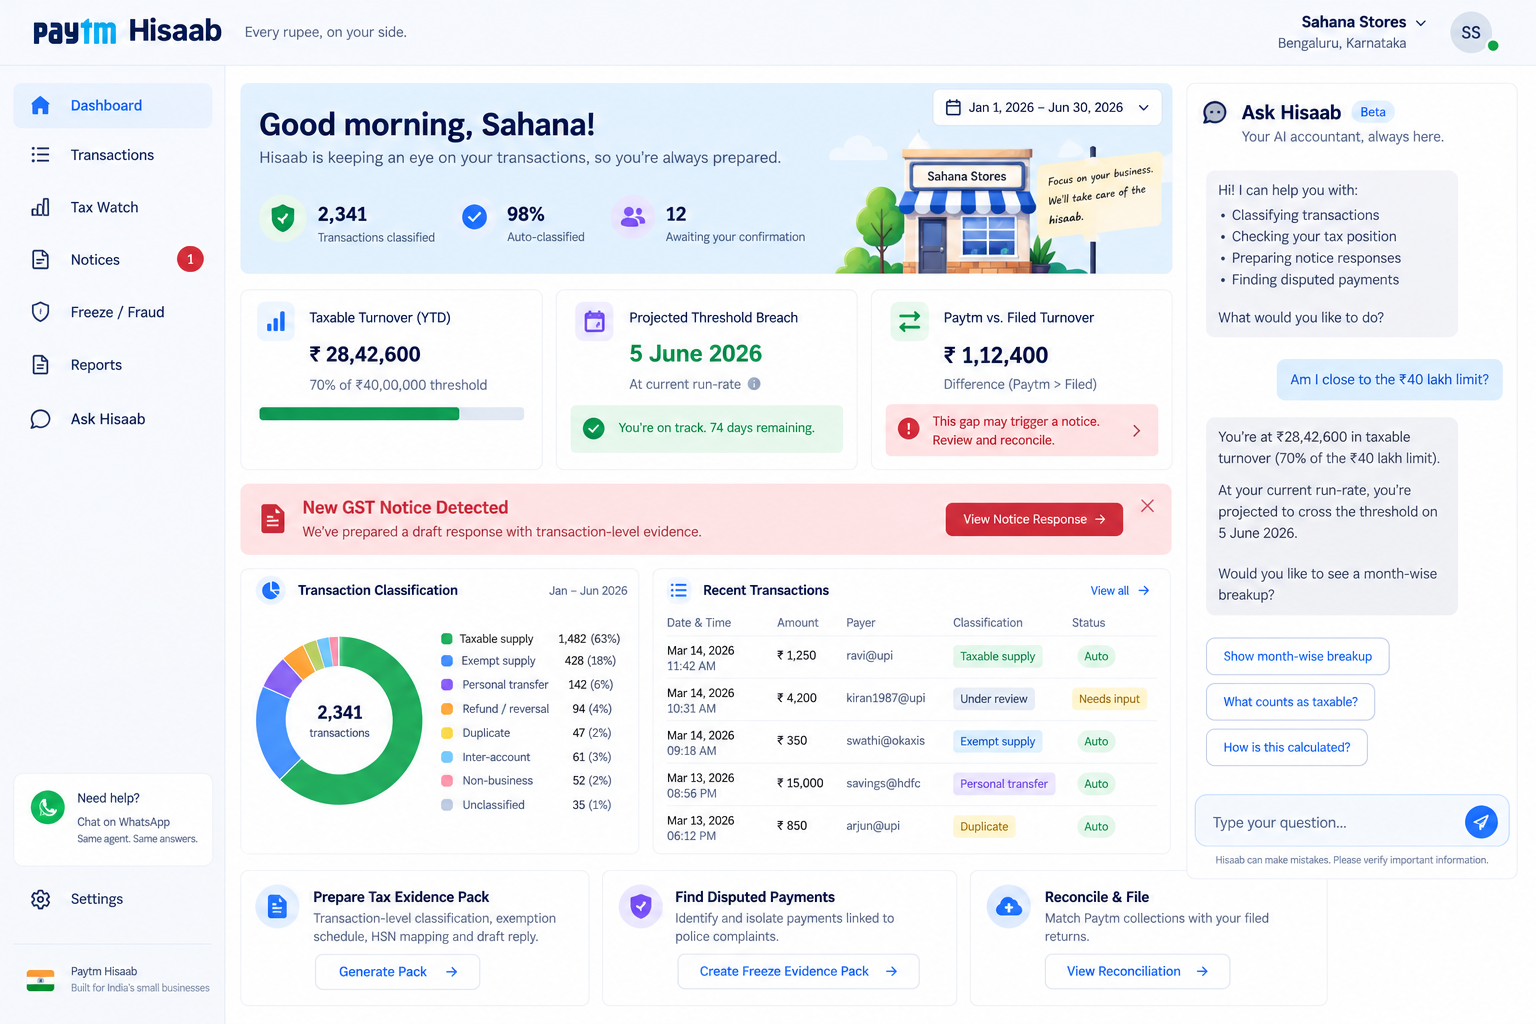
\includegraphics[width=\textwidth,height=0.70\textheight,keepaspectratio]{Paytm-Hisaab_website_look.png}
\end{center}
\vspace{0.1cm}
\hspace{0.05cm}{\scriptsize\color{muted}One surface: what every payment was classified as, how close she is to the threshold, and the packs. The same agent runs on WhatsApp, where she actually is.}
\note{{\color{navy}\bfseries\normalsize 8.~What the merchant sees}\par\vspace{0.55em}\textbf{0:20 --- a glance slide. Do not tour the UI.}
\\[0.4em]
One sentence: everything classified, how close she is to the threshold, and the
packs, on one surface.
\\[0.4em]
Then the WhatsApp point --- the same agent, where she actually is --- and advance.
\\[0.4em]
If someone asks whether this is built: the chat and the tools are live; this
screen is the product surface we are designing toward.}
\end{frame}

% ============================================================ 9. ARCHITECTURE
\begin{frame}{Built on Phinite}{Two agent graphs, four agents, ten deterministic skills}
\vspace{0.15cm}
\begin{columns}[T]
\begin{column}{0.53\textwidth}
{\scriptsize
\begin{tabular}{@{}L{1.75cm}L{4.7cm}@{}}
\multicolumn{2}{@{}l}{\color{navy}\bfseries\small hisaab-watch \;\scriptsize(autonomous: cron + API)}\\
\midrule
Provenance & proposes a tag and a reason for the hard credits \\
Evidence   & assembles packs: freeze evidence, then exemption schedules and HSN \\
\addlinespace[0.6em]
\multicolumn{2}{@{}l}{\color{navy}\bfseries\small hisaab-merchant \;\scriptsize(conversational: chat)}\\
\midrule
Merchant   & the conversation: attestation, alerts, Kannada \\
Escalation & decides when to stop and route to a human CA \\
\bottomrule
\end{tabular}}
\\[0.75em]
{\scriptsize\color{muted}The nightly pass writes its queue to the ledger; the chat reads it when she opens it. Deliberately \emph{not} a graph-to-graph call: a queue that outlives either run is what makes the handoff robust.}
\end{column}
\begin{column}{0.44\textwidth}
\card{5.7cm}{{\bfseries\color{navy}Permissions are the product}\\[0.4em]
\scriptsize Provenance proposes, \red{never commits}.\\[0.25em]
\scriptsize Merchant is the \emph{only} agent that can commit a tag.\\[0.25em]
\scriptsize Evidence is \red{read-only}. It cannot edit a classification to make a pack look better.\\[0.25em]
\scriptsize Escalation can \red{halt} any pack; a human approves.}
\\[0.5em]
\hspace{0.1cm}\begin{minipage}{5.7cm}{\scriptsize\color{muted}Ten tools run live against a hosted service. Every number in a pack traces back, in the trace, to the credit and the attestation behind it.}\end{minipage}
\end{column}
\end{columns}
\note{{\color{navy}\bfseries\normalsize 9.~Built on Phinite}\par\vspace{0.55em}\textbf{0:40 --- for the technical judges.}
\\[0.4em]
Two agent graphs, not four loose agents: \texttt{hisaab-watch} runs autonomously on
cron, \texttt{hisaab-merchant} is the conversation. The nightly pass writes a queue;
the chat reads it when she opens it --- deliberately not a graph-to-graph call,
because a queue that outlives either run is what makes the handoff robust.
\\[0.4em]
\textbf{Spend your time on the right-hand card.} The strongest line in it:
the Evidence agent is read-only --- \emph{the agent that builds the defence cannot
edit the evidence.} And only the Merchant agent can commit an attested tag.
\\[0.4em]
Those are enforced as Phinite tool policies, not conventions, and a denied call
shows up in the trace.}
\end{frame}

% ============================================================ 10. DESIGN DECISIONS
\begin{frame}{Four decisions that make it defensible}
\vspace{0.3cm}
\begin{columns}[T]
\begin{column}{0.48\textwidth}
\card{6.0cm}{{\bfseries\color{navy}1. Arithmetic lives in skills, not the model}\\[0.35em]
\scriptsize Turnover, projections and apportionment are deterministic Python: versioned, testable, traceable. Wrapping arithmetic in an LLM is the standard tell, and the trace would show it.}
\\[0.35em]
\card{6.0cm}{{\bfseries\color{navy}3. Refusing to guess is a feature}\\[0.35em]
\scriptsize An \texttt{unclassified} credit routed to the merchant costs one tap. A confident wrong tag inside an evidence pack is a catastrophe. We report the refusal rate honestly.}
\end{column}
\begin{column}{0.48\textwidth}
\card{6.0cm}{{\bfseries\color{navy}2. Attestation is the promotion boundary}\\[0.35em]
\scriptsize Nothing enters a production pack that the merchant has not confirmed. Sandbox to UAT to prod, with her tap as the gate.}
\\[0.35em]
\card{6.0cm}{{\bfseries\color{navy}4. Ground truth, so accuracy is a number}\\[0.35em]
\scriptsize We simulated a year of a shop's life from a known process, split into what Paytm can see and what really happened. Agents read only the visible half, which is why we quote error bars instead of vibes.}
\end{column}
\end{columns}
\note{{\color{navy}\bfseries\normalsize 10.~Four decisions}\par\vspace{0.55em}\textbf{0:35 --- the slide that separates you from a demo.}
\\[0.4em]
Lead with \#1: all arithmetic is deterministic Python, not model output. Wrapping
arithmetic in an LLM is the standard tell, and the trace would show it.
\\[0.4em]
Then \#3: refusing to guess is a feature. An \texttt{unclassified} credit costs one
tap; a confident wrong tag inside an evidence pack is a catastrophe.
\\[0.4em]
Skim \#2 and \#4 --- one clause each. \#4 is worth a beat if the room is technical:
we generated ground truth, so accuracy is a number instead of a claim.}
\end{frame}

% ============================================================ 11. DEMO / ATTESTATION
\begin{frame}{Demo $\cdot$ Sahana Stores, Jayanagar}{An ordinary Tuesday, before anything goes wrong}
\vspace{0.1cm}
\begin{columns}[T]
\begin{column}{0.48\textwidth}
{\scriptsize\color{muted}Tuesday 10 March. Thirty-nine credits came in over the weekend. The agent asks about \hi{three}.}
\\[0.4em]
\card{5.9cm}{{\kn\scriptsize ಭಾನುವಾರ ರಾತ್ರಿ ₹15,000. ನಿಮ್ಮ ಸ್ವಂತ ಹಣವೇ?}\\[0.25em]
{\color{muted}\scriptsize \qm{₹15,000 at 11:04pm Sunday, from your savings account. Your own money?}}\\[0.35em]
{\scriptsize\color{navy}\fbox{\kn ಹೌದು}\;\fbox{\kn ಇಲ್ಲ}}}
\\[0.4em]
{\scriptsize $\cdot$\; ₹7,500 from her husband, scanned at the shop QR\\[0.25em]
$\cdot$\; ₹4,850 from Raghu Shetty, who has bought twice before. A real sale, and the agent \emph{asks} rather than assumes.}
\\[0.4em]
{\scriptsize\color{muted}The other thirty-six settle silently, and a ₹23 payment nobody can place is left alone.}
\end{column}
\begin{column}{0.48\textwidth}
\ocard{amber}{6.1cm}{{\bfseries\color{amber}And yes, two of those three should not be there}\\[0.35em]
\scriptsize A business QR is not for personal money, and the terms say so. It arrives anyway: family, own top-ups, a chit payout. The rule does not prevent it. It only means \emph{nobody keeps a record of it.}}
\\[0.45em]
{\scriptsize Paytm already reads the signals: channel, linked VPAs, payer history. What no system has is the \hi{merchant's own answer}, given at the time, in her language, and kept.}
\\[0.45em]
{\scriptsize That record is what the next two slides are built from: first for the police, then for the department.}
\end{column}
\end{columns}
\note{{\color{navy}\bfseries\normalsize 11.~Demo --- an ordinary Tuesday (beat 1)}\par\vspace{0.55em}\textbf{0:45 --- or hand over to the live demo here.}
\\[0.4em]
Thirty-nine credits came in over the weekend, the agent asks about \textbf{three}.
Read the Kannada line if you can; otherwise read the gloss under it.
\\[0.4em]
\textbf{Do not hide from the right-hand card --- lead with it.} The mid-review
point was that personal money is not allowed on a business QR. Correct, and we say
so on the slide. The argument is that the rule does not stop it, it only means no
one records it, and an unrecorded credit is what an authority later reads as income.
\\[0.4em]
\textbf{Second half of that card matters just as much.} We are not claiming Paytm
does nothing. It already reads channel, linked VPAs and payer history. What no
system has is her own answer, captured while it is still knowable. That is the
product, and it is a smaller, truer claim than the one we started with.
\\[0.4em]
\textbf{Before going on stage:} confirm the attestation queue is whole ---
\texttt{pending\_total} must be 3. A rehearsal that taps through this beat spends the
queue, and Render needs a clear-cache redeploy to restore it.}
\end{frame}

% ============================================================ 12. DEMO / THE FREEZE
\begin{frame}{Demo $\cdot$ The emergency}{The account is frozen at 09:30 and the supplier payment is due}
\vspace{0.2cm}
\begin{columns}[T]
\begin{column}{0.46\textwidth}
{\scriptsize She sold someone 12kg of onions. That customer was three layers downstream of a fraud victim. She is not named in the FIR, which was filed in another state, and \hi{339 payments} came in that week.}
\\[0.5em]
\card{5.8cm}{{\bfseries\color{navy}The agent isolates it}\\[0.35em]
\scriptsize ₹4,200 on 21 March at 19:47, till POS01. Matched by UTR \emph{and independently} by amount and date.\\[0.3em]
\scriptsize The sale record comes with it: the POS bill, the items, the till and the minute.}
\end{column}
\begin{column}{0.49\textwidth}
\ocard{amber}{6.1cm}{{\bfseries\color{amber}And the decoy it did not choose}\\[0.35em]
\scriptsize A \emph{second} ₹4,200 that same week, from a regular customer. Listed in the pack, and explicitly \emph{not} named as the disputed one. Only the date separates them.}
\\[0.5em]
{\scriptsize Then it drafts the NCRP-CFCFRMS grievance, citing the judgments that only the \emph{disputed amount} should be lien-marked, not the whole account.}
\\[0.5em]
{\scriptsize\color{bad}\bfseries It never asserts that she is innocent.}\\[0.1em]
{\scriptsize\color{muted}Some frozen accounts genuinely are mule accounts. The agent assembles evidence; a human decides. Escalation holds the pack for approval.}
\end{column}
\end{columns}
\note{{\color{navy}\bfseries\normalsize 12.~Demo --- the emergency (beat 4)}\par\vspace{0.55em}\textbf{0:50 --- this is now the lead case. Give it the most time of the three.}
\\[0.4em]
Set the stakes in one sentence: account frozen at half nine, supplier payment due,
339 payments came in that week, and she is not named in the FIR.
\\[0.4em]
\textbf{Why this one leads.} She did nothing wrong and there is no rule she broke.
She sold onions to a customer who turned out to be laundering. Every objection
available against the tax case --- she should not have taken personal money on that
QR, she should have registered --- has no purchase here at all.
\\[0.4em]
The agent isolates ₹4,200 by UTR \emph{and independently} by amount and date, and
brings the POS bill with it --- the items, till POS01, 19:47.
\\[0.4em]
\textbf{The decoy is the point.} A second ₹4,200 that same week from a regular
customer, listed in the pack and explicitly not chosen. Anyone can match an amount;
the pack shows its work.
\\[0.4em]
Finish on the red line: it never asserts she is innocent. Some frozen accounts
genuinely are mule accounts. We assemble evidence; a human decides, and Escalation
holds the pack for approval.}
\end{frame}

% ============================================================ 13. DEMO / TAX
\begin{frame}{Demo $\cdot$ The warning, and the notice}{The same ledger, read for the other authority}
\vspace{0.15cm}
\begin{columns}[T]
\begin{column}{0.38\textwidth}
{\scriptsize\color{muted}Replayed as of 31 January:}
\\[0.35em]
\ocard{good}{4.8cm}{{\bfseries\color{ink}\scriptsize\qm{At your current rate you cross ₹40 lakh around {\color{bad}14 March}. You will need to register.}}\\[0.35em]
{\scriptsize\color{muted}\grn{43 days of warning}, and the date is computed, not typed.}}
\\[0.45em]
{\scriptsize\color{bad}\bfseries This beat is what makes the pitch safe.}\\[0.1em]
{\scriptsize\color{muted}Its first act on the tax side is telling her to register.}
\end{column}
\begin{column}{0.58\textwidth}
{\scriptsize\color{muted}Then the notice arrives, claiming {\color{bad}\bfseries ₹60.98L} of turnover:}
\\[0.3em]
{\scriptsize
\begin{tabular}{@{}lr@{\hskip 1.2em}l@{}}
\multicolumn{2}{@{}l}{\color{navy}\bfseries Aggregate turnover \quad ₹42.2L} & \sub{within \grn{1.6\%} of truth} \\
\midrule
Exempt supplies      & ₹31.3L & \sub{vegetables, loose rice} \\
Taxable supplies     & ₹10.9L & \sub{branded goods, oil, soap} \\
\addlinespace[0.45em]
\multicolumn{2}{@{}l}{\color{navy}\bfseries Not turnover at all \quad ₹18.8L} & \sub{every line traced} \\
\midrule
Her own accounts     & ₹7.4L & \sub{top-ups before supplier runs} \\
Family               & ₹6.1L & \sub{spouse, parent, in-law} \\
Loans, chit, gifts   & ₹4.3L & \sub{chit payout, festival gifts} \\
Refunds, duplicates  & ₹1.0L & \sub{crate returns, double-taps} \\
\bottomrule
\end{tabular}}
\\[0.45em]
{\scriptsize And it says plainly: \hi{the claim is wrong, and you \emph{did} cross ₹40 lakh on 14 March. You must register.}}
\end{column}
\end{columns}
\note{{\color{navy}\bfseries\normalsize 13.~Demo --- the warning and the notice (beats 2 and 3)}\par\vspace{0.55em}\textbf{0:50 --- two tax beats on one slide, deliberately compressed.}
\\[0.4em]
Left: replayed as of 31 January, the agent says she crosses ₹40 lakh around
14 March. \textbf{Say the red line out loud} --- its first act on the tax side is
telling her she owes a registration. That is what stops the room turning hostile.
\\[0.4em]
Right: the notice claims ₹60.98 lakh, and the pack answers it line by line, every
figure traceable to transaction IDs. Then the honest half:
\textbf{the claim is wrong, and she did cross ₹40 lakh, and she must register.}
\\[0.4em]
\textbf{If a judge diffs this against slide 5:} slide 5 shows seeded truth
(₹42.9L), this shows what our system computed (₹42.2L). The 1.6\% between them
\emph{is} the accuracy claim --- say that, do not hedge.
\\[0.4em]
\textbf{If pushed on the personal and own-account lines:} same answer as slide 11.
Those credits should not be on a business QR, they are there anyway, and the
alternative to classifying them is letting them be read as income.}
\end{frame}

% ============================================================ 14. NUMBERS
\begin{frame}{What we can actually prove}{One merchant, one year, 13,267 credits, scored against seeded truth}
\vspace{0.45cm}
\begin{columns}[T]
\begin{column}{0.33\textwidth}
\begin{center}\bignum{1.6\%}{error on aggregate turnover\\ (taxable share within 1\%)}\end{center}
\vspace{0.55cm}
\begin{center}\bignum{43 days}{of warning before the\\ threshold crossing}\end{center}
\end{column}
\begin{column}{0.33\textwidth}
\begin{center}\bignum{1.3 a day}{median questions asked.\\ 189 in a year, never over 3}\end{center}
\vspace{0.55cm}
\begin{center}\bignum{zero}{credits left untagged\\ across the whole year}\end{center}
\end{column}
\begin{column}{0.30\textwidth}
\card{3.8cm}{{\bfseries\color{navy}The honest baseline}\\[0.35em]
\scriptsize A 50-line rules-only classifier gets 99.3\% on sale vs not-a-sale, but catches only \red{77.8\%} of non-sale credits.\\[0.3em]
\scriptsize That residue alone puts two eval merchants on the \emph{wrong side} of ₹40L.\\[0.3em]
\scriptsize Closing it is what the agent plus one tap is for.}
\end{column}
\end{columns}
\vspace{0.45cm}
\hspace{0.1cm}{\scriptsize\color{muted}She corrected the agent 52 times that year. Those corrections are the ledger's strongest evidence, not its failures.}
\note{{\color{navy}\bfseries\normalsize 14.~What we can actually prove}\par\vspace{0.55em}\textbf{0:30 --- do not read all four. Pick two.}
\\[0.4em]
Lead with \textbf{1.6\%} error on turnover and \textbf{1.3 questions a day}. The
other two are there to be read, not narrated.
\\[0.4em]
\textbf{The credibility move is the box on the right} --- volunteer the weakness
before anyone finds it. A rules-only baseline gets 99.3\% on sale vs not-a-sale
but catches only 77.8\% of non-sale credits, and that residue alone puts two eval
merchants on the wrong side of ₹40 lakh. Closing it is what the agent plus one tap is for.
\\[0.4em]
Last line if you have the beat: she corrected the agent 52 times that year, and
those corrections are the ledger's strongest evidence, not its failures.}
\end{frame}

% ============================================================ 15. CLOSE
\begin{frame}{The line we do not cross}{Accuracy, not minimisation}
\vspace{0.3cm}
\begin{columns}[T]
\begin{column}{0.52\textwidth}
{\scriptsize
$\cdot$\; We \hi{never assert innocence} on a freeze. Some accounts really are mule accounts. We assemble evidence; a human decides.\\[0.5em]
$\cdot$\; We \hi{file nothing} with any authority. Artefacts only; the merchant or their CA files.\\[0.5em]
$\cdot$\; We compute what she \hi{genuinely owes} and say so plainly, including \qm{you crossed the threshold, you must register.}\\[0.5em]
$\cdot$\; We \hi{never assert a final liability}. We compute, show the workings, and route to a CA.\\[0.5em]
$\cdot$\; A business QR is \hi{not for personal money}. We do not excuse it. We record it, so it is not read as income.}
\end{column}
\begin{column}{0.44\textwidth}
\begin{tikzpicture}\node[rounded corners=4pt,fill=navy,text=white,inner sep=10pt,text width=5.7cm,align=left]{
{\bfseries Why this has to be Paytm}\\[0.45em]
\scriptsize The rail is the only place provenance is cheap. Everyone else arrives eighteen months late, when the answer is already unrecoverable.\\[0.45em]
\scriptsize A frozen merchant cannot transact at all: dead Soundbox and zero GMV the same morning, before it becomes the sign on the shutter, \emph{\qm{No UPI. Cash only.}}
};\end{tikzpicture}
\end{column}
\end{columns}
\vspace{0.4cm}
\begin{center}
{\large\color{navy}\bfseries Paytm Hisaab}\quad{\color{muted}every rupee, on your side.}
\end{center}
\note{{\color{navy}\bfseries\normalsize 15.~The line we do not cross}\par\vspace{0.55em}\textbf{0:30 --- the non-negotiables, fast, then land.}
\\[0.4em]
Run the five bullets at pace. The one to hit is the first: we never assert
innocence on a freeze. The last is the mid-review answer, on the slide on purpose.
\\[0.4em]
Then the navy box: provenance is cheap only on the rail, and a frozen merchant
stops transacting the same morning.
\\[0.4em]
Final line, unhurried: \emph{``Paytm Hisaab. Every rupee, on your side.''} Stop talking.
\\[0.5em]
{\scriptsize
{\color{navy}\bfseries --- Q\&A prep ---}
\\[0.3em]
\textbf{``Merchants may not take personal money on a business QR.''} Correct, and
slide 11 says so before you have to. It arrives anyway, and the alternative to
recording it is letting an authority read it as income. We are not defending the
behaviour --- we are refusing to let it become a liability.
\\[0.3em]
\textbf{``Paytm already tags transactions.''} It does, and we build on that rather
than around it: channel, linked VPAs and payer history feed the rules layer. What
no tag carries is her attestation --- the part an authority accepts, and the only
part she alone can give.
\\[0.3em]
\textbf{``No return mismatch?''} That check needs a \emph{registered} composition
dealer who filed a CMP-08 to disagree with. Ours is unregistered, which is why she
gets a notice at all; the eval split has one with four quarters seeded.
\\[0.3em]
\textbf{``Exempt vs taxable on a QR sale?''} Not per payment. We apportion by value
from that shop's own POS-billed ratio and label it an estimate. Labelling each sale
by its majority side understated taxable turnover threefold.
\\[0.3em]
\textbf{``Four LLM calls in a trenchcoat?''} Everything deterministic is a skill and
four agents is the ceiling. If twenty lines of Python replaces an agent, it should
have been a skill --- the trace shows which is which.
\\[0.3em]
\textbf{``No standing with the police.''} Agreed: Paytm supplies, the merchant
files. By design. Cash sales are real, out of scope, and on the slide.}}
\end{frame}

\end{document}
